\documentclass{book}
\usepackage[a4paper,top=2.5cm,bottom=2.5cm,left=2.5cm,right=2.5cm]{geometry}
\usepackage{makeidx}
\usepackage{natbib}
\usepackage{graphicx}
\usepackage{multicol}
\usepackage{float}
\usepackage{listings}
\usepackage{color}
\usepackage{ifthen}
\usepackage[table]{xcolor}
\usepackage{textcomp}
\usepackage{alltt}
\usepackage{ifpdf}
\ifpdf
\usepackage[pdftex,
            pagebackref=true,
            colorlinks=true,
            linkcolor=blue,
            unicode
           ]{hyperref}
\else
\usepackage[ps2pdf,
            pagebackref=true,
            colorlinks=true,
            linkcolor=blue,
            unicode
           ]{hyperref}
\usepackage{pspicture}
\fi
\usepackage[utf8]{inputenc}
\usepackage{mathptmx}
\usepackage[scaled=.90]{helvet}
\usepackage{courier}
\usepackage{sectsty}
\usepackage{amssymb}
\usepackage[titles]{tocloft}
\usepackage{doxygen}
\lstset{language=C++,inputencoding=utf8,basicstyle=\footnotesize,breaklines=true,breakatwhitespace=true,tabsize=4,numbers=left }
\makeindex
\setcounter{tocdepth}{3}
\renewcommand{\footrulewidth}{0.4pt}
\renewcommand{\familydefault}{\sfdefault}
\hfuzz=15pt
\setlength{\emergencystretch}{15pt}
\hbadness=750
\tolerance=750
\begin{document}
\hypersetup{pageanchor=false,citecolor=blue}
\begin{titlepage}
\vspace*{7cm}
\begin{center}
{\Large Social\-Network Analysis Engine }\\
\vspace*{1cm}
{\large Generated by Doxygen 1.8.3.1}\\
\vspace*{0.5cm}
{\small Thu Mar 14 2013 17:48:45}\\
\end{center}
\end{titlepage}
\clearemptydoublepage
\pagenumbering{roman}
\tableofcontents
\clearemptydoublepage
\pagenumbering{arabic}
\hypersetup{pageanchor=true,citecolor=blue}
\chapter{Namespace Index}
\section{Namespace List}
Here is a list of all namespaces with brief descriptions\-:\begin{DoxyCompactList}
\item\contentsline{section}{\hyperlink{namespacesaedb}{saedb} }{\pageref{d9/dc5/namespacesaedb}}{}
\end{DoxyCompactList}

\chapter{Hierarchical Index}
\section{Class Hierarchy}
This inheritance list is sorted roughly, but not completely, alphabetically\-:\begin{DoxyCompactList}
\item \contentsline{section}{saedb\-:\-:graph\-\_\-storage$<$ Vertex\-Data, Edge\-Data $>$\-:\-:edge\-\_\-info}{\pageref{da/d12/classsaedb_1_1graph__storage_1_1edge__info}}{}
\item \contentsline{section}{saedb\-:\-:graph\-\_\-storage$<$ Vertex\-Data, Edge\-Data $>$\-:\-:edge\-\_\-iterator}{\pageref{d8/d8a/classsaedb_1_1graph__storage_1_1edge__iterator}}{}
\item \contentsline{section}{saedb\-:\-:graph\-\_\-storage$<$ Vertex\-Data, Edge\-Data $>$\-:\-:edge\-\_\-list}{\pageref{d3/d38/classsaedb_1_1graph__storage_1_1edge__list}}{}
\item \contentsline{section}{saedb\-:\-:local\-\_\-graph$<$ Vertex\-Data, Edge\-Data $>$\-:\-:edge\-\_\-type}{\pageref{da/d9c/structsaedb_1_1local__graph_1_1edge__type}}{}
\item \contentsline{section}{saedb\-:\-:sae\-\_\-graph$<$ Vertex\-Data, Edge\-Data $>$\-:\-:edge\-\_\-type}{\pageref{d0/db8/classsaedb_1_1sae__graph_1_1edge__type}}{}
\item \contentsline{section}{saedb\-:\-:graph\-\_\-storage$<$ Vertex\-Data, Edge\-Data $>$\-:\-:edge\-\_\-type}{\pageref{df/d01/classsaedb_1_1graph__storage_1_1edge__type}}{}
\item \contentsline{section}{saedb\-:\-:empty}{\pageref{d6/d3f/structsaedb_1_1empty}}{}
\item \contentsline{section}{saedb\-:\-:graph\-\_\-storage$<$ Vertex\-Data, Edge\-Data $>$}{\pageref{db/dd8/classsaedb_1_1graph__storage}}{}
\item \contentsline{section}{saedb\-:\-:icontext$<$ Graph\-Type, Gather\-Type, Message\-Type $>$}{\pageref{d6/d73/classsaedb_1_1icontext}}{}
\item \contentsline{section}{saedb\-:\-:icontext$<$ Engine\-:\-:graph\-\_\-type, Engine\-:\-:gather\-\_\-type, Engine\-:\-:message\-\_\-type $>$}{\pageref{d6/d73/classsaedb_1_1icontext}}{}
\begin{DoxyCompactList}
\item \contentsline{section}{saedb\-:\-:context$<$ Engine $>$}{\pageref{d1/d89/classsaedb_1_1context}}{}
\end{DoxyCompactList}
\item \contentsline{section}{saedb\-:\-:sae\-\_\-graph$<$ Vertex\-Data, Edge\-Data $>$\-:\-:local\-\_\-edge\-\_\-list\-\_\-type}{\pageref{d7/dec/structsaedb_1_1sae__graph_1_1local__edge__list__type}}{}
\item \contentsline{section}{saedb\-:\-:sae\-\_\-graph$<$ Vertex\-Data, Edge\-Data $>$\-:\-:local\-\_\-edge\-\_\-type}{\pageref{d1/d46/classsaedb_1_1sae__graph_1_1local__edge__type}}{}
\item \contentsline{section}{saedb\-:\-:local\-\_\-graph$<$ Vertex\-Data, Edge\-Data $>$}{\pageref{d9/d4a/classsaedb_1_1local__graph}}{}
\item \contentsline{section}{saedb\-:\-:sae\-\_\-graph$<$ Vertex\-Data, Edge\-Data $>$\-:\-:local\-\_\-vertex\-\_\-type}{\pageref{d7/d91/structsaedb_1_1sae__graph_1_1local__vertex__type}}{}
\item \contentsline{section}{saedb\-:\-:sae\-\_\-algorithm$<$ Graph, Gather\-Type, Message\-Type $>$}{\pageref{d0/d9f/classsaedb_1_1sae__algorithm}}{}
\item \contentsline{section}{saedb\-:\-:sae\-\_\-algorithm$<$ graph\-\_\-type, float $>$}{\pageref{d0/d9f/classsaedb_1_1sae__algorithm}}{}
\begin{DoxyCompactList}
\item \contentsline{section}{pagerank}{\pageref{d7/d39/classpagerank}}{}
\item \contentsline{section}{pagerank}{\pageref{d7/d39/classpagerank}}{}
\item \contentsline{section}{pagerank}{\pageref{d7/d39/classpagerank}}{}
\end{DoxyCompactList}
\item \contentsline{section}{saedb\-:\-:sae\-\_\-engine$<$ Vertex\-Program\-Type $>$}{\pageref{d9/d3c/classsaedb_1_1sae__engine}}{}
\item \contentsline{section}{saedb\-:\-:sae\-\_\-engine$<$ Vertex\-Program $>$}{\pageref{d9/d3c/classsaedb_1_1sae__engine}}{}
\begin{DoxyCompactList}
\item \contentsline{section}{saedb\-:\-:sae\-\_\-synchronous\-\_\-engine$<$ Vertex\-Program $>$}{\pageref{d7/d39/classsaedb_1_1sae__synchronous__engine}}{}
\end{DoxyCompactList}
\item \contentsline{section}{saedb\-:\-:sae\-\_\-graph$<$ Vertex\-Data, Edge\-Data $>$}{\pageref{d6/d2b/classsaedb_1_1sae__graph}}{}
\item \contentsline{section}{saedb\-:\-:sae\-\_\-graph$<$ Vertex\-Data, Edge\-Data $>$\-:\-:vertex\-\_\-type}{\pageref{d1/d90/structsaedb_1_1sae__graph_1_1vertex__type}}{}
\item \contentsline{section}{saedb\-:\-:local\-\_\-graph$<$ Vertex\-Data, Edge\-Data $>$\-:\-:vertex\-\_\-type}{\pageref{dd/d9a/structsaedb_1_1local__graph_1_1vertex__type}}{}
\end{DoxyCompactList}

\chapter{Class Index}
\section{Class List}
Here are the classes, structs, unions and interfaces with brief descriptions\-:\begin{DoxyCompactList}
\item\contentsline{section}{\hyperlink{classsaedb_1_1context}{saedb\-::context$<$ Engine $>$} }{\pageref{d1/d89/classsaedb_1_1context}}{}
\item\contentsline{section}{\hyperlink{classsaedb_1_1graph__storage_1_1edge__info}{saedb\-::graph\-\_\-storage$<$ Vertex\-Data, Edge\-Data $>$\-::edge\-\_\-info} }{\pageref{da/d12/classsaedb_1_1graph__storage_1_1edge__info}}{}
\item\contentsline{section}{\hyperlink{classsaedb_1_1graph__storage_1_1edge__iterator}{saedb\-::graph\-\_\-storage$<$ Vertex\-Data, Edge\-Data $>$\-::edge\-\_\-iterator} }{\pageref{d8/d8a/classsaedb_1_1graph__storage_1_1edge__iterator}}{}
\item\contentsline{section}{\hyperlink{classsaedb_1_1graph__storage_1_1edge__list}{saedb\-::graph\-\_\-storage$<$ Vertex\-Data, Edge\-Data $>$\-::edge\-\_\-list} }{\pageref{d3/d38/classsaedb_1_1graph__storage_1_1edge__list}}{}
\item\contentsline{section}{\hyperlink{structsaedb_1_1local__graph_1_1edge__type}{saedb\-::local\-\_\-graph$<$ Vertex\-Data, Edge\-Data $>$\-::edge\-\_\-type} }{\pageref{da/d9c/structsaedb_1_1local__graph_1_1edge__type}}{}
\item\contentsline{section}{\hyperlink{classsaedb_1_1sae__graph_1_1edge__type}{saedb\-::sae\-\_\-graph$<$ Vertex\-Data, Edge\-Data $>$\-::edge\-\_\-type} }{\pageref{d0/db8/classsaedb_1_1sae__graph_1_1edge__type}}{}
\item\contentsline{section}{\hyperlink{classsaedb_1_1graph__storage_1_1edge__type}{saedb\-::graph\-\_\-storage$<$ Vertex\-Data, Edge\-Data $>$\-::edge\-\_\-type} }{\pageref{df/d01/classsaedb_1_1graph__storage_1_1edge__type}}{}
\item\contentsline{section}{\hyperlink{structsaedb_1_1empty}{saedb\-::empty} }{\pageref{d6/d3f/structsaedb_1_1empty}}{}
\item\contentsline{section}{\hyperlink{classsaedb_1_1graph__storage}{saedb\-::graph\-\_\-storage$<$ Vertex\-Data, Edge\-Data $>$} }{\pageref{db/dd8/classsaedb_1_1graph__storage}}{}
\item\contentsline{section}{\hyperlink{classsaedb_1_1icontext}{saedb\-::icontext$<$ Graph\-Type, Gather\-Type, Message\-Type $>$} }{\pageref{d6/d73/classsaedb_1_1icontext}}{}
\item\contentsline{section}{\hyperlink{structsaedb_1_1sae__graph_1_1local__edge__list__type}{saedb\-::sae\-\_\-graph$<$ Vertex\-Data, Edge\-Data $>$\-::local\-\_\-edge\-\_\-list\-\_\-type} }{\pageref{d7/dec/structsaedb_1_1sae__graph_1_1local__edge__list__type}}{}
\item\contentsline{section}{\hyperlink{classsaedb_1_1sae__graph_1_1local__edge__type}{saedb\-::sae\-\_\-graph$<$ Vertex\-Data, Edge\-Data $>$\-::local\-\_\-edge\-\_\-type} }{\pageref{d1/d46/classsaedb_1_1sae__graph_1_1local__edge__type}}{}
\item\contentsline{section}{\hyperlink{classsaedb_1_1local__graph}{saedb\-::local\-\_\-graph$<$ Vertex\-Data, Edge\-Data $>$} }{\pageref{d9/d4a/classsaedb_1_1local__graph}}{}
\item\contentsline{section}{\hyperlink{structsaedb_1_1sae__graph_1_1local__vertex__type}{saedb\-::sae\-\_\-graph$<$ Vertex\-Data, Edge\-Data $>$\-::local\-\_\-vertex\-\_\-type} }{\pageref{d7/d91/structsaedb_1_1sae__graph_1_1local__vertex__type}}{}
\item\contentsline{section}{\hyperlink{classpagerank}{pagerank} }{\pageref{d7/d39/classpagerank}}{}
\item\contentsline{section}{\hyperlink{classsaedb_1_1sae__algorithm}{saedb\-::sae\-\_\-algorithm$<$ Graph, Gather\-Type, Message\-Type $>$} }{\pageref{d0/d9f/classsaedb_1_1sae__algorithm}}{}
\item\contentsline{section}{\hyperlink{classsaedb_1_1sae__engine}{saedb\-::sae\-\_\-engine$<$ Vertex\-Program\-Type $>$} }{\pageref{d9/d3c/classsaedb_1_1sae__engine}}{}
\item\contentsline{section}{\hyperlink{classsaedb_1_1sae__graph}{saedb\-::sae\-\_\-graph$<$ Vertex\-Data, Edge\-Data $>$} }{\pageref{d6/d2b/classsaedb_1_1sae__graph}}{}
\item\contentsline{section}{\hyperlink{classsaedb_1_1sae__synchronous__engine}{saedb\-::sae\-\_\-synchronous\-\_\-engine$<$ Vertex\-Program $>$} }{\pageref{d7/d39/classsaedb_1_1sae__synchronous__engine}}{}
\item\contentsline{section}{\hyperlink{structsaedb_1_1sae__graph_1_1vertex__type}{saedb\-::sae\-\_\-graph$<$ Vertex\-Data, Edge\-Data $>$\-::vertex\-\_\-type} }{\pageref{d1/d90/structsaedb_1_1sae__graph_1_1vertex__type}}{}
\item\contentsline{section}{\hyperlink{structsaedb_1_1local__graph_1_1vertex__type}{saedb\-::local\-\_\-graph$<$ Vertex\-Data, Edge\-Data $>$\-::vertex\-\_\-type} }{\pageref{dd/d9a/structsaedb_1_1local__graph_1_1vertex__type}}{}
\end{DoxyCompactList}

\chapter{File Index}
\section{File List}
Here is a list of all files with brief descriptions\-:\begin{DoxyCompactList}
\item\contentsline{section}{src/\hyperlink{helloworld_8cpp}{helloworld.\-cpp} }{\pageref{db/d67/helloworld_8cpp}}{}
\item\contentsline{section}{src/app/basic/clustering/\hyperlink{kmeans_8cpp}{kmeans.\-cpp} }{\pageref{d3/dfb/kmeans_8cpp}}{}
\item\contentsline{section}{src/app/basic/pagerank/\hyperlink{basic_2pagerank_2pagerank_8cpp}{pagerank.\-cpp} }{\pageref{da/d99/basic_2pagerank_2pagerank_8cpp}}{}
\item\contentsline{section}{src/app/demo/pagerank/\hyperlink{demo_2pagerank_2pagerank_8cpp}{pagerank.\-cpp} }{\pageref{db/de9/demo_2pagerank_2pagerank_8cpp}}{}
\item\contentsline{section}{src/saedb/\hyperlink{context_8hpp}{context.\-hpp} }{\pageref{d2/da3/context_8hpp}}{}
\item\contentsline{section}{src/saedb/\hyperlink{engine_8hpp}{engine.\-hpp} }{\pageref{de/d46/engine_8hpp}}{}
\item\contentsline{section}{src/saedb/\hyperlink{graph_8hpp}{graph.\-hpp} }{\pageref{d9/de9/graph_8hpp}}{}
\item\contentsline{section}{src/saedb/\hyperlink{graph__basic__types_8cpp}{graph\-\_\-basic\-\_\-types.\-cpp} }{\pageref{d2/d6d/graph__basic__types_8cpp}}{}
\item\contentsline{section}{src/saedb/\hyperlink{graph__storage_8hpp}{graph\-\_\-storage.\-hpp} }{\pageref{dc/d95/graph__storage_8hpp}}{}
\item\contentsline{section}{src/saedb/\hyperlink{icontext_8hpp}{icontext.\-hpp} }{\pageref{d6/d8b/icontext_8hpp}}{}
\item\contentsline{section}{src/saedb/\hyperlink{local__graph_8hpp}{local\-\_\-graph.\-hpp} }{\pageref{d1/d93/local__graph_8hpp}}{}
\item\contentsline{section}{src/saedb/\hyperlink{sae__include_8hpp}{sae\-\_\-include.\-hpp} }{\pageref{d4/dc7/sae__include_8hpp}}{}
\item\contentsline{section}{src/saedb/\hyperlink{synchronous__engine_8cpp}{synchronous\-\_\-engine.\-cpp} }{\pageref{df/dda/synchronous__engine_8cpp}}{}
\item\contentsline{section}{src/saedb/\hyperlink{vertex__program_8hpp}{vertex\-\_\-program.\-hpp} }{\pageref{de/d9a/vertex__program_8hpp}}{}
\end{DoxyCompactList}

\chapter{Namespace Documentation}
\hypertarget{namespacesaedb}{\section{saedb Namespace Reference}
\label{d9/dc5/namespacesaedb}\index{saedb@{saedb}}
}
\subsection*{Classes}
\begin{DoxyCompactItemize}
\item 
class \hyperlink{classsaedb_1_1context}{context}
\item 
class \hyperlink{classsaedb_1_1sae__engine}{sae\-\_\-engine}
\item 
class \hyperlink{classsaedb_1_1sae__graph}{sae\-\_\-graph}
\item 
struct \hyperlink{structsaedb_1_1empty}{empty}
\item 
class \hyperlink{classsaedb_1_1graph__storage}{graph\-\_\-storage}
\item 
class \hyperlink{classsaedb_1_1icontext}{icontext}
\item 
class \hyperlink{classsaedb_1_1local__graph}{local\-\_\-graph}
\item 
class \hyperlink{classsaedb_1_1sae__synchronous__engine}{sae\-\_\-synchronous\-\_\-engine}
\item 
class \hyperlink{classsaedb_1_1sae__algorithm}{sae\-\_\-algorithm}
\end{DoxyCompactItemize}
\subsection*{Typedefs}
\begin{DoxyCompactItemize}
\item 
typedef uint32\-\_\-t \hyperlink{namespacesaedb_a502e07e24003e811ae3bd73514c2798a}{vertex\-\_\-id\-\_\-type}
\item 
typedef uint32\-\_\-t \hyperlink{namespacesaedb_ae0f2df508bdfd29505d57534c8ed4a65}{lvid\-\_\-type}
\item 
typedef \hyperlink{namespacesaedb_ae0f2df508bdfd29505d57534c8ed4a65}{lvid\-\_\-type} \hyperlink{namespacesaedb_af76c9a21f199f95828dd18699754cad1}{edge\-\_\-id\-\_\-type}
\end{DoxyCompactItemize}
\subsection*{Enumerations}
\begin{DoxyCompactItemize}
\item 
enum \hyperlink{namespacesaedb_adf5ad13c09a48fb2f42f8e7348ea3ac3}{edge\-\_\-dir\-\_\-type} \{ \hyperlink{namespacesaedb_adf5ad13c09a48fb2f42f8e7348ea3ac3a9fff15c8a891e45b0e19a4f164b7f93f}{N\-O\-\_\-\-E\-D\-G\-E\-S}, 
\hyperlink{namespacesaedb_adf5ad13c09a48fb2f42f8e7348ea3ac3a71ec98c5ef3686233cdcd0234fbdffe5}{I\-N\-\_\-\-E\-D\-G\-E\-S}, 
\hyperlink{namespacesaedb_adf5ad13c09a48fb2f42f8e7348ea3ac3a7e77290ddb5b73f4ed2d39a9627c2786}{O\-U\-T\-\_\-\-E\-D\-G\-E\-S}, 
\hyperlink{namespacesaedb_adf5ad13c09a48fb2f42f8e7348ea3ac3a49d613a86fc84d8a45d95ecd1354912e}{A\-L\-L\-\_\-\-E\-D\-G\-E\-S}
 \}
\end{DoxyCompactItemize}
\subsection*{Functions}
\begin{DoxyCompactItemize}
\item 
{\footnotesize template$<$typename to $>$ }\\void \hyperlink{namespacesaedb_ae9fdd1f0012c6fc9946f2dc123fe90e0}{log} (to t)
\end{DoxyCompactItemize}


\subsection{Detailed Description}
not used now 

\subsection{Typedef Documentation}
\hypertarget{namespacesaedb_af76c9a21f199f95828dd18699754cad1}{\index{saedb@{saedb}!edge\-\_\-id\-\_\-type@{edge\-\_\-id\-\_\-type}}
\index{edge\-\_\-id\-\_\-type@{edge\-\_\-id\-\_\-type}!saedb@{saedb}}
\subsubsection[{edge\-\_\-id\-\_\-type}]{\setlength{\rightskip}{0pt plus 5cm}typedef {\bf lvid\-\_\-type} {\bf saedb\-::edge\-\_\-id\-\_\-type}}}\label{d9/dc5/namespacesaedb_af76c9a21f199f95828dd18699754cad1}


Definition at line 10 of file graph\-\_\-basic\-\_\-types.\-cpp.

\hypertarget{namespacesaedb_ae0f2df508bdfd29505d57534c8ed4a65}{\index{saedb@{saedb}!lvid\-\_\-type@{lvid\-\_\-type}}
\index{lvid\-\_\-type@{lvid\-\_\-type}!saedb@{saedb}}
\subsubsection[{lvid\-\_\-type}]{\setlength{\rightskip}{0pt plus 5cm}typedef uint32\-\_\-t {\bf saedb\-::lvid\-\_\-type}}}\label{d9/dc5/namespacesaedb_ae0f2df508bdfd29505d57534c8ed4a65}


Definition at line 8 of file graph\-\_\-basic\-\_\-types.\-cpp.

\hypertarget{namespacesaedb_a502e07e24003e811ae3bd73514c2798a}{\index{saedb@{saedb}!vertex\-\_\-id\-\_\-type@{vertex\-\_\-id\-\_\-type}}
\index{vertex\-\_\-id\-\_\-type@{vertex\-\_\-id\-\_\-type}!saedb@{saedb}}
\subsubsection[{vertex\-\_\-id\-\_\-type}]{\setlength{\rightskip}{0pt plus 5cm}typedef uint32\-\_\-t {\bf saedb\-::vertex\-\_\-id\-\_\-type}}}\label{d9/dc5/namespacesaedb_a502e07e24003e811ae3bd73514c2798a}


Definition at line 6 of file graph\-\_\-basic\-\_\-types.\-cpp.



\subsection{Enumeration Type Documentation}
\hypertarget{namespacesaedb_adf5ad13c09a48fb2f42f8e7348ea3ac3}{\index{saedb@{saedb}!edge\-\_\-dir\-\_\-type@{edge\-\_\-dir\-\_\-type}}
\index{edge\-\_\-dir\-\_\-type@{edge\-\_\-dir\-\_\-type}!saedb@{saedb}}
\subsubsection[{edge\-\_\-dir\-\_\-type}]{\setlength{\rightskip}{0pt plus 5cm}enum {\bf saedb\-::edge\-\_\-dir\-\_\-type}}}\label{d9/dc5/namespacesaedb_adf5ad13c09a48fb2f42f8e7348ea3ac3}
\begin{Desc}
\item[Enumerator]\par
\begin{description}
\index{N\-O\-\_\-\-E\-D\-G\-E\-S@{N\-O\-\_\-\-E\-D\-G\-E\-S}!saedb@{saedb}}\index{saedb@{saedb}!N\-O\-\_\-\-E\-D\-G\-E\-S@{N\-O\-\_\-\-E\-D\-G\-E\-S}}\item[{\em 
\hypertarget{namespacesaedb_adf5ad13c09a48fb2f42f8e7348ea3ac3a9fff15c8a891e45b0e19a4f164b7f93f}{N\-O\-\_\-\-E\-D\-G\-E\-S}\label{d9/dc5/namespacesaedb_adf5ad13c09a48fb2f42f8e7348ea3ac3a9fff15c8a891e45b0e19a4f164b7f93f}
}]\index{I\-N\-\_\-\-E\-D\-G\-E\-S@{I\-N\-\_\-\-E\-D\-G\-E\-S}!saedb@{saedb}}\index{saedb@{saedb}!I\-N\-\_\-\-E\-D\-G\-E\-S@{I\-N\-\_\-\-E\-D\-G\-E\-S}}\item[{\em 
\hypertarget{namespacesaedb_adf5ad13c09a48fb2f42f8e7348ea3ac3a71ec98c5ef3686233cdcd0234fbdffe5}{I\-N\-\_\-\-E\-D\-G\-E\-S}\label{d9/dc5/namespacesaedb_adf5ad13c09a48fb2f42f8e7348ea3ac3a71ec98c5ef3686233cdcd0234fbdffe5}
}]\index{O\-U\-T\-\_\-\-E\-D\-G\-E\-S@{O\-U\-T\-\_\-\-E\-D\-G\-E\-S}!saedb@{saedb}}\index{saedb@{saedb}!O\-U\-T\-\_\-\-E\-D\-G\-E\-S@{O\-U\-T\-\_\-\-E\-D\-G\-E\-S}}\item[{\em 
\hypertarget{namespacesaedb_adf5ad13c09a48fb2f42f8e7348ea3ac3a7e77290ddb5b73f4ed2d39a9627c2786}{O\-U\-T\-\_\-\-E\-D\-G\-E\-S}\label{d9/dc5/namespacesaedb_adf5ad13c09a48fb2f42f8e7348ea3ac3a7e77290ddb5b73f4ed2d39a9627c2786}
}]\index{A\-L\-L\-\_\-\-E\-D\-G\-E\-S@{A\-L\-L\-\_\-\-E\-D\-G\-E\-S}!saedb@{saedb}}\index{saedb@{saedb}!A\-L\-L\-\_\-\-E\-D\-G\-E\-S@{A\-L\-L\-\_\-\-E\-D\-G\-E\-S}}\item[{\em 
\hypertarget{namespacesaedb_adf5ad13c09a48fb2f42f8e7348ea3ac3a49d613a86fc84d8a45d95ecd1354912e}{A\-L\-L\-\_\-\-E\-D\-G\-E\-S}\label{d9/dc5/namespacesaedb_adf5ad13c09a48fb2f42f8e7348ea3ac3a49d613a86fc84d8a45d95ecd1354912e}
}]\end{description}
\end{Desc}


Definition at line 12 of file graph\-\_\-basic\-\_\-types.\-cpp.



\subsection{Function Documentation}
\hypertarget{namespacesaedb_ae9fdd1f0012c6fc9946f2dc123fe90e0}{\index{saedb@{saedb}!log@{log}}
\index{log@{log}!saedb@{saedb}}
\subsubsection[{log}]{\setlength{\rightskip}{0pt plus 5cm}template$<$typename to $>$ void saedb\-::log (
\begin{DoxyParamCaption}
\item[{to}]{t}
\end{DoxyParamCaption}
)}}\label{d9/dc5/namespacesaedb_ae9fdd1f0012c6fc9946f2dc123fe90e0}


Definition at line 79 of file synchronous\-\_\-engine.\-cpp.


\chapter{Class Documentation}
\hypertarget{classsaedb_1_1context}{\section{saedb\-:\-:context$<$ Engine $>$ Class Template Reference}
\label{d1/d89/classsaedb_1_1context}\index{saedb\-::context$<$ Engine $>$@{saedb\-::context$<$ Engine $>$}}
}


{\ttfamily \#include $<$context.\-hpp$>$}

Inheritance diagram for saedb\-:\-:context$<$ Engine $>$\-:\begin{figure}[H]
\begin{center}
\leavevmode
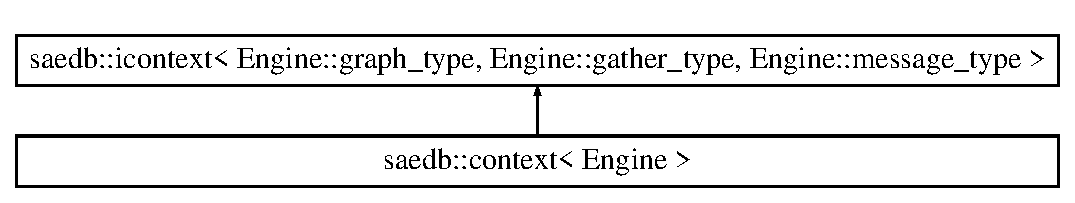
\includegraphics[height=2.000000cm]{d1/d89/classsaedb_1_1context}
\end{center}
\end{figure}
\subsection*{Public Types}
\begin{DoxyCompactItemize}
\item 
typedef Engine \hyperlink{classsaedb_1_1context_a10f237a9463e78f60b333d7017cbf948}{engine\-\_\-type}
\item 
typedef \hyperlink{classsaedb_1_1icontext}{icontext}$<$ typename \\*
\hyperlink{demo_2pagerank_2pagerank_8cpp_afa42a4da0de8450a5bb4145aa06ee689}{Engine\-::graph\-\_\-type}, typename \\*
Engine\-::gather\-\_\-type, typename \\*
Engine\-::message\-\_\-type $>$ \hyperlink{classsaedb_1_1context_ae9df8581f3061e5caa9272039d969b18}{icontext\-\_\-type}
\item 
typedef \hyperlink{classsaedb_1_1icontext_a8eeb99ff6eb90e3f096a2895f9b92653}{icontext\-\_\-type\-::graph\-\_\-type} \hyperlink{classsaedb_1_1context_af74463841aa837f915f43fce2ca64dca}{graph\-\_\-type}
\item 
typedef \\*
\hyperlink{classsaedb_1_1icontext_ac130cf374063f27748e4770617971660}{icontext\-\_\-type\-::vertex\-\_\-id\-\_\-type} \hyperlink{classsaedb_1_1context_aba9540d1189edf19f3d1cb7363b5c40b}{vertex\-\_\-id\-\_\-type}
\item 
typedef \hyperlink{classsaedb_1_1icontext_ab83a38ba860cb2101b499ae60675e4e5}{icontext\-\_\-type\-::vertex\-\_\-type} \hyperlink{classsaedb_1_1context_a62f418b2b73082cd65a88feb604bab9f}{vertex\-\_\-type}
\item 
typedef \hyperlink{classsaedb_1_1icontext_a7bd82d8486ab08dc1adf49dd6d659059}{icontext\-\_\-type\-::message\-\_\-type} \hyperlink{classsaedb_1_1context_ad29784e44db80b03b0adab9a2d8f2c72}{message\-\_\-type}
\item 
typedef \hyperlink{classsaedb_1_1icontext_a7c3ae1019b418faf3de68ab9396f867b}{icontext\-\_\-type\-::gather\-\_\-type} \hyperlink{classsaedb_1_1context_acce022e81537ee830f3df623f4f9e0d4}{gather\-\_\-type}
\end{DoxyCompactItemize}
\subsection*{Public Member Functions}
\begin{DoxyCompactItemize}
\item 
\hyperlink{classsaedb_1_1context_ac2248694285b99cf6fa359bf4a7ddb28}{context} (\hyperlink{classsaedb_1_1context_a10f237a9463e78f60b333d7017cbf948}{engine\-\_\-type} \&engine, \hyperlink{classsaedb_1_1context_af74463841aa837f915f43fce2ca64dca}{graph\-\_\-type} \&graph)
\begin{DoxyCompactList}\small\item\em Construct a context for a particular engine and graph pair. \end{DoxyCompactList}\item 
size\-\_\-t \hyperlink{classsaedb_1_1context_a19833a898006e8618b5f1a449569e64b}{num\-\_\-vertices} () const 
\item 
size\-\_\-t \hyperlink{classsaedb_1_1context_aa33ef2cb3e708b0eca6b502f3c962897}{num\-\_\-edges} () const 
\item 
size\-\_\-t \hyperlink{classsaedb_1_1context_a09b1e692a0b01ffb61e6abf6f5ba3c5d}{procid} () const 
\item 
size\-\_\-t \hyperlink{classsaedb_1_1context_aaa4630b0aca2bbde0167428cff7ab7e6}{num\-\_\-procs} () const 
\item 
std\-::ostream \& \hyperlink{classsaedb_1_1context_a66c19922ee1b6f5bd61ab022f2f4622a}{cout} () const 
\item 
std\-::ostream \& \hyperlink{classsaedb_1_1context_ab01112333512c57d6dc0156b6c807b99}{cerr} () const 
\item 
float \hyperlink{classsaedb_1_1context_a582c3612423e18a6891e78d96e1cc5cb}{elapsed\-\_\-seconds} () const 
\item 
int \hyperlink{classsaedb_1_1context_a0c6faad7f4c09a5a90acd58b6a413f97}{iteration} () const 
\item 
void \hyperlink{classsaedb_1_1context_a6337795d74509e592457f5d4f992573b}{stop} ()
\item 
void \hyperlink{classsaedb_1_1context_a86002f3e0ce79e720421575847cf00ac}{signal} (const \hyperlink{classsaedb_1_1context_a62f418b2b73082cd65a88feb604bab9f}{vertex\-\_\-type} \&vertex, const \hyperlink{classsaedb_1_1context_ad29784e44db80b03b0adab9a2d8f2c72}{message\-\_\-type} \&message=\hyperlink{classsaedb_1_1context_ad29784e44db80b03b0adab9a2d8f2c72}{message\-\_\-type}())
\item 
void \hyperlink{classsaedb_1_1context_a64e80cac06f3df77ca818d760c05d6c6}{signal\-\_\-vid} (\hyperlink{classsaedb_1_1context_aba9540d1189edf19f3d1cb7363b5c40b}{vertex\-\_\-id\-\_\-type} vid, const \hyperlink{classsaedb_1_1context_ad29784e44db80b03b0adab9a2d8f2c72}{message\-\_\-type} \&message=\hyperlink{classsaedb_1_1context_ad29784e44db80b03b0adab9a2d8f2c72}{message\-\_\-type}())
\item 
void \hyperlink{classsaedb_1_1context_aa623eb9e9aa1fc82ff0dbffbfc80619f}{post\-\_\-delta} (const \hyperlink{classsaedb_1_1context_a62f418b2b73082cd65a88feb604bab9f}{vertex\-\_\-type} \&vertex, const \hyperlink{classsaedb_1_1context_acce022e81537ee830f3df623f4f9e0d4}{gather\-\_\-type} \&delta)
\item 
virtual void \hyperlink{classsaedb_1_1context_a1654f9e7e61601ebe886c760d4170c59}{clear\-\_\-gather\-\_\-cache} (const \hyperlink{classsaedb_1_1context_a62f418b2b73082cd65a88feb604bab9f}{vertex\-\_\-type} \&vertex)
\end{DoxyCompactItemize}


\subsection{Detailed Description}
\subsubsection*{template$<$typename Engine$>$class saedb\-::context$<$ Engine $>$}



Definition at line 13 of file context.\-hpp.



\subsection{Member Typedef Documentation}
\hypertarget{classsaedb_1_1context_a10f237a9463e78f60b333d7017cbf948}{\index{saedb\-::context@{saedb\-::context}!engine\-\_\-type@{engine\-\_\-type}}
\index{engine\-\_\-type@{engine\-\_\-type}!saedb::context@{saedb\-::context}}
\subsubsection[{engine\-\_\-type}]{\setlength{\rightskip}{0pt plus 5cm}template$<$typename Engine $>$ typedef Engine {\bf saedb\-::context}$<$ Engine $>$\-::{\bf engine\-\_\-type}}}\label{d1/d89/classsaedb_1_1context_a10f237a9463e78f60b333d7017cbf948}
The engine that created this context object 

Definition at line 20 of file context.\-hpp.

\hypertarget{classsaedb_1_1context_acce022e81537ee830f3df623f4f9e0d4}{\index{saedb\-::context@{saedb\-::context}!gather\-\_\-type@{gather\-\_\-type}}
\index{gather\-\_\-type@{gather\-\_\-type}!saedb::context@{saedb\-::context}}
\subsubsection[{gather\-\_\-type}]{\setlength{\rightskip}{0pt plus 5cm}template$<$typename Engine $>$ typedef {\bf icontext\-\_\-type\-::gather\-\_\-type} {\bf saedb\-::context}$<$ Engine $>$\-::{\bf gather\-\_\-type}}}\label{d1/d89/classsaedb_1_1context_acce022e81537ee830f3df623f4f9e0d4}


Definition at line 30 of file context.\-hpp.

\hypertarget{classsaedb_1_1context_af74463841aa837f915f43fce2ca64dca}{\index{saedb\-::context@{saedb\-::context}!graph\-\_\-type@{graph\-\_\-type}}
\index{graph\-\_\-type@{graph\-\_\-type}!saedb::context@{saedb\-::context}}
\subsubsection[{graph\-\_\-type}]{\setlength{\rightskip}{0pt plus 5cm}template$<$typename Engine $>$ typedef {\bf icontext\-\_\-type\-::graph\-\_\-type} {\bf saedb\-::context}$<$ Engine $>$\-::{\bf graph\-\_\-type}}}\label{d1/d89/classsaedb_1_1context_af74463841aa837f915f43fce2ca64dca}


Definition at line 26 of file context.\-hpp.

\hypertarget{classsaedb_1_1context_ae9df8581f3061e5caa9272039d969b18}{\index{saedb\-::context@{saedb\-::context}!icontext\-\_\-type@{icontext\-\_\-type}}
\index{icontext\-\_\-type@{icontext\-\_\-type}!saedb::context@{saedb\-::context}}
\subsubsection[{icontext\-\_\-type}]{\setlength{\rightskip}{0pt plus 5cm}template$<$typename Engine $>$ typedef {\bf icontext}$<$typename {\bf Engine\-::graph\-\_\-type}, typename Engine\-::gather\-\_\-type, typename Engine\-::message\-\_\-type$>$ {\bf saedb\-::context}$<$ Engine $>$\-::{\bf icontext\-\_\-type}}}\label{d1/d89/classsaedb_1_1context_ae9df8581f3061e5caa9272039d969b18}
The parent type 

Definition at line 25 of file context.\-hpp.

\hypertarget{classsaedb_1_1context_ad29784e44db80b03b0adab9a2d8f2c72}{\index{saedb\-::context@{saedb\-::context}!message\-\_\-type@{message\-\_\-type}}
\index{message\-\_\-type@{message\-\_\-type}!saedb::context@{saedb\-::context}}
\subsubsection[{message\-\_\-type}]{\setlength{\rightskip}{0pt plus 5cm}template$<$typename Engine $>$ typedef {\bf icontext\-\_\-type\-::message\-\_\-type} {\bf saedb\-::context}$<$ Engine $>$\-::{\bf message\-\_\-type}}}\label{d1/d89/classsaedb_1_1context_ad29784e44db80b03b0adab9a2d8f2c72}


Definition at line 29 of file context.\-hpp.

\hypertarget{classsaedb_1_1context_aba9540d1189edf19f3d1cb7363b5c40b}{\index{saedb\-::context@{saedb\-::context}!vertex\-\_\-id\-\_\-type@{vertex\-\_\-id\-\_\-type}}
\index{vertex\-\_\-id\-\_\-type@{vertex\-\_\-id\-\_\-type}!saedb::context@{saedb\-::context}}
\subsubsection[{vertex\-\_\-id\-\_\-type}]{\setlength{\rightskip}{0pt plus 5cm}template$<$typename Engine $>$ typedef {\bf icontext\-\_\-type\-::vertex\-\_\-id\-\_\-type} {\bf saedb\-::context}$<$ Engine $>$\-::{\bf vertex\-\_\-id\-\_\-type}}}\label{d1/d89/classsaedb_1_1context_aba9540d1189edf19f3d1cb7363b5c40b}


Definition at line 27 of file context.\-hpp.

\hypertarget{classsaedb_1_1context_a62f418b2b73082cd65a88feb604bab9f}{\index{saedb\-::context@{saedb\-::context}!vertex\-\_\-type@{vertex\-\_\-type}}
\index{vertex\-\_\-type@{vertex\-\_\-type}!saedb::context@{saedb\-::context}}
\subsubsection[{vertex\-\_\-type}]{\setlength{\rightskip}{0pt plus 5cm}template$<$typename Engine $>$ typedef {\bf icontext\-\_\-type\-::vertex\-\_\-type} {\bf saedb\-::context}$<$ Engine $>$\-::{\bf vertex\-\_\-type}}}\label{d1/d89/classsaedb_1_1context_a62f418b2b73082cd65a88feb604bab9f}


Definition at line 28 of file context.\-hpp.



\subsection{Constructor \& Destructor Documentation}
\hypertarget{classsaedb_1_1context_ac2248694285b99cf6fa359bf4a7ddb28}{\index{saedb\-::context@{saedb\-::context}!context@{context}}
\index{context@{context}!saedb::context@{saedb\-::context}}
\subsubsection[{context}]{\setlength{\rightskip}{0pt plus 5cm}template$<$typename Engine $>$ {\bf saedb\-::context}$<$ Engine $>$\-::{\bf context} (
\begin{DoxyParamCaption}
\item[{{\bf engine\-\_\-type} \&}]{engine, }
\item[{{\bf graph\-\_\-type} \&}]{graph}
\end{DoxyParamCaption}
)\hspace{0.3cm}{\ttfamily [inline]}}}\label{d1/d89/classsaedb_1_1context_ac2248694285b99cf6fa359bf4a7ddb28}


Construct a context for a particular engine and graph pair. 



Definition at line 44 of file context.\-hpp.



\subsection{Member Function Documentation}
\hypertarget{classsaedb_1_1context_ab01112333512c57d6dc0156b6c807b99}{\index{saedb\-::context@{saedb\-::context}!cerr@{cerr}}
\index{cerr@{cerr}!saedb::context@{saedb\-::context}}
\subsubsection[{cerr}]{\setlength{\rightskip}{0pt plus 5cm}template$<$typename Engine $>$ std\-::ostream\& {\bf saedb\-::context}$<$ Engine $>$\-::cerr (
\begin{DoxyParamCaption}
{}
\end{DoxyParamCaption}
) const\hspace{0.3cm}{\ttfamily [inline]}, {\ttfamily [virtual]}}}\label{d1/d89/classsaedb_1_1context_ab01112333512c57d6dc0156b6c807b99}


Reimplemented from \hyperlink{classsaedb_1_1icontext_a056142a0edfabcdcd0254a7003dcfd84}{saedb\-::icontext$<$ Engine\-::graph\-\_\-type, Engine\-::gather\-\_\-type, Engine\-::message\-\_\-type $>$}.



Definition at line 67 of file context.\-hpp.

\hypertarget{classsaedb_1_1context_a1654f9e7e61601ebe886c760d4170c59}{\index{saedb\-::context@{saedb\-::context}!clear\-\_\-gather\-\_\-cache@{clear\-\_\-gather\-\_\-cache}}
\index{clear\-\_\-gather\-\_\-cache@{clear\-\_\-gather\-\_\-cache}!saedb::context@{saedb\-::context}}
\subsubsection[{clear\-\_\-gather\-\_\-cache}]{\setlength{\rightskip}{0pt plus 5cm}template$<$typename Engine $>$ virtual void {\bf saedb\-::context}$<$ Engine $>$\-::clear\-\_\-gather\-\_\-cache (
\begin{DoxyParamCaption}
\item[{const {\bf vertex\-\_\-type} \&}]{vertex}
\end{DoxyParamCaption}
)\hspace{0.3cm}{\ttfamily [inline]}, {\ttfamily [virtual]}}}\label{d1/d89/classsaedb_1_1context_a1654f9e7e61601ebe886c760d4170c59}
Invalidate the cached gather on the vertex. 

Reimplemented from \hyperlink{classsaedb_1_1icontext_a327a0e7c8b3b040abb577715e1844c14}{saedb\-::icontext$<$ Engine\-::graph\-\_\-type, Engine\-::gather\-\_\-type, Engine\-::message\-\_\-type $>$}.



Definition at line 114 of file context.\-hpp.

\hypertarget{classsaedb_1_1context_a66c19922ee1b6f5bd61ab022f2f4622a}{\index{saedb\-::context@{saedb\-::context}!cout@{cout}}
\index{cout@{cout}!saedb::context@{saedb\-::context}}
\subsubsection[{cout}]{\setlength{\rightskip}{0pt plus 5cm}template$<$typename Engine $>$ std\-::ostream\& {\bf saedb\-::context}$<$ Engine $>$\-::cout (
\begin{DoxyParamCaption}
{}
\end{DoxyParamCaption}
) const\hspace{0.3cm}{\ttfamily [inline]}, {\ttfamily [virtual]}}}\label{d1/d89/classsaedb_1_1context_a66c19922ee1b6f5bd61ab022f2f4622a}


Reimplemented from \hyperlink{classsaedb_1_1icontext_aebcd170e0a7f73c5c23ccc2c5109c8ad}{saedb\-::icontext$<$ Engine\-::graph\-\_\-type, Engine\-::gather\-\_\-type, Engine\-::message\-\_\-type $>$}.



Definition at line 64 of file context.\-hpp.

\hypertarget{classsaedb_1_1context_a582c3612423e18a6891e78d96e1cc5cb}{\index{saedb\-::context@{saedb\-::context}!elapsed\-\_\-seconds@{elapsed\-\_\-seconds}}
\index{elapsed\-\_\-seconds@{elapsed\-\_\-seconds}!saedb::context@{saedb\-::context}}
\subsubsection[{elapsed\-\_\-seconds}]{\setlength{\rightskip}{0pt plus 5cm}template$<$typename Engine $>$ float {\bf saedb\-::context}$<$ Engine $>$\-::elapsed\-\_\-seconds (
\begin{DoxyParamCaption}
{}
\end{DoxyParamCaption}
) const\hspace{0.3cm}{\ttfamily [inline]}, {\ttfamily [virtual]}}}\label{d1/d89/classsaedb_1_1context_a582c3612423e18a6891e78d96e1cc5cb}
Get the elapsed time in seconds 

Reimplemented from \hyperlink{classsaedb_1_1icontext_a4c8cc12932257edf89e97ec3e462c113}{saedb\-::icontext$<$ Engine\-::graph\-\_\-type, Engine\-::gather\-\_\-type, Engine\-::message\-\_\-type $>$}.



Definition at line 73 of file context.\-hpp.

\hypertarget{classsaedb_1_1context_a0c6faad7f4c09a5a90acd58b6a413f97}{\index{saedb\-::context@{saedb\-::context}!iteration@{iteration}}
\index{iteration@{iteration}!saedb::context@{saedb\-::context}}
\subsubsection[{iteration}]{\setlength{\rightskip}{0pt plus 5cm}template$<$typename Engine $>$ int {\bf saedb\-::context}$<$ Engine $>$\-::iteration (
\begin{DoxyParamCaption}
{}
\end{DoxyParamCaption}
) const\hspace{0.3cm}{\ttfamily [inline]}, {\ttfamily [virtual]}}}\label{d1/d89/classsaedb_1_1context_a0c6faad7f4c09a5a90acd58b6a413f97}
Return the current interation number (if supported). 

Reimplemented from \hyperlink{classsaedb_1_1icontext_a3d56a20cb9b5e48a76a1cdaba0b0f944}{saedb\-::icontext$<$ Engine\-::graph\-\_\-type, Engine\-::gather\-\_\-type, Engine\-::message\-\_\-type $>$}.



Definition at line 78 of file context.\-hpp.

\hypertarget{classsaedb_1_1context_aa33ef2cb3e708b0eca6b502f3c962897}{\index{saedb\-::context@{saedb\-::context}!num\-\_\-edges@{num\-\_\-edges}}
\index{num\-\_\-edges@{num\-\_\-edges}!saedb::context@{saedb\-::context}}
\subsubsection[{num\-\_\-edges}]{\setlength{\rightskip}{0pt plus 5cm}template$<$typename Engine $>$ size\-\_\-t {\bf saedb\-::context}$<$ Engine $>$\-::num\-\_\-edges (
\begin{DoxyParamCaption}
{}
\end{DoxyParamCaption}
) const\hspace{0.3cm}{\ttfamily [inline]}, {\ttfamily [virtual]}}}\label{d1/d89/classsaedb_1_1context_aa33ef2cb3e708b0eca6b502f3c962897}
Get the number of edges in the graph 

Reimplemented from \hyperlink{classsaedb_1_1icontext_aa0ea9bf7ccdbd58a7fec6fe6b124f14b}{saedb\-::icontext$<$ Engine\-::graph\-\_\-type, Engine\-::gather\-\_\-type, Engine\-::message\-\_\-type $>$}.



Definition at line 52 of file context.\-hpp.

\hypertarget{classsaedb_1_1context_aaa4630b0aca2bbde0167428cff7ab7e6}{\index{saedb\-::context@{saedb\-::context}!num\-\_\-procs@{num\-\_\-procs}}
\index{num\-\_\-procs@{num\-\_\-procs}!saedb::context@{saedb\-::context}}
\subsubsection[{num\-\_\-procs}]{\setlength{\rightskip}{0pt plus 5cm}template$<$typename Engine $>$ size\-\_\-t {\bf saedb\-::context}$<$ Engine $>$\-::num\-\_\-procs (
\begin{DoxyParamCaption}
{}
\end{DoxyParamCaption}
) const\hspace{0.3cm}{\ttfamily [inline]}, {\ttfamily [virtual]}}}\label{d1/d89/classsaedb_1_1context_aaa4630b0aca2bbde0167428cff7ab7e6}


Reimplemented from \hyperlink{classsaedb_1_1icontext_a7ae74263673ec0aeda4765a936ca20ad}{saedb\-::icontext$<$ Engine\-::graph\-\_\-type, Engine\-::gather\-\_\-type, Engine\-::message\-\_\-type $>$}.



Definition at line 62 of file context.\-hpp.

\hypertarget{classsaedb_1_1context_a19833a898006e8618b5f1a449569e64b}{\index{saedb\-::context@{saedb\-::context}!num\-\_\-vertices@{num\-\_\-vertices}}
\index{num\-\_\-vertices@{num\-\_\-vertices}!saedb::context@{saedb\-::context}}
\subsubsection[{num\-\_\-vertices}]{\setlength{\rightskip}{0pt plus 5cm}template$<$typename Engine $>$ size\-\_\-t {\bf saedb\-::context}$<$ Engine $>$\-::num\-\_\-vertices (
\begin{DoxyParamCaption}
{}
\end{DoxyParamCaption}
) const\hspace{0.3cm}{\ttfamily [inline]}, {\ttfamily [virtual]}}}\label{d1/d89/classsaedb_1_1context_a19833a898006e8618b5f1a449569e64b}


Reimplemented from \hyperlink{classsaedb_1_1icontext_ad40db46945f6dfbd6e738d0206298b76}{saedb\-::icontext$<$ Engine\-::graph\-\_\-type, Engine\-::gather\-\_\-type, Engine\-::message\-\_\-type $>$}.



Definition at line 47 of file context.\-hpp.

\hypertarget{classsaedb_1_1context_aa623eb9e9aa1fc82ff0dbffbfc80619f}{\index{saedb\-::context@{saedb\-::context}!post\-\_\-delta@{post\-\_\-delta}}
\index{post\-\_\-delta@{post\-\_\-delta}!saedb::context@{saedb\-::context}}
\subsubsection[{post\-\_\-delta}]{\setlength{\rightskip}{0pt plus 5cm}template$<$typename Engine $>$ void {\bf saedb\-::context}$<$ Engine $>$\-::post\-\_\-delta (
\begin{DoxyParamCaption}
\item[{const {\bf vertex\-\_\-type} \&}]{vertex, }
\item[{const {\bf gather\-\_\-type} \&}]{delta}
\end{DoxyParamCaption}
)\hspace{0.3cm}{\ttfamily [inline]}}}\label{d1/d89/classsaedb_1_1context_aa623eb9e9aa1fc82ff0dbffbfc80619f}
Post a change to the cached sum for the vertex 

Definition at line 107 of file context.\-hpp.

\hypertarget{classsaedb_1_1context_a09b1e692a0b01ffb61e6abf6f5ba3c5d}{\index{saedb\-::context@{saedb\-::context}!procid@{procid}}
\index{procid@{procid}!saedb::context@{saedb\-::context}}
\subsubsection[{procid}]{\setlength{\rightskip}{0pt plus 5cm}template$<$typename Engine $>$ size\-\_\-t {\bf saedb\-::context}$<$ Engine $>$\-::procid (
\begin{DoxyParamCaption}
{}
\end{DoxyParamCaption}
) const\hspace{0.3cm}{\ttfamily [inline]}, {\ttfamily [virtual]}}}\label{d1/d89/classsaedb_1_1context_a09b1e692a0b01ffb61e6abf6f5ba3c5d}
Get an estimate of the number of update functions executed up to this point. 

Reimplemented from \hyperlink{classsaedb_1_1icontext_a806cf7e2a500cde5c58c9b35d3614e02}{saedb\-::icontext$<$ Engine\-::graph\-\_\-type, Engine\-::gather\-\_\-type, Engine\-::message\-\_\-type $>$}.



Definition at line 60 of file context.\-hpp.

\hypertarget{classsaedb_1_1context_a86002f3e0ce79e720421575847cf00ac}{\index{saedb\-::context@{saedb\-::context}!signal@{signal}}
\index{signal@{signal}!saedb::context@{saedb\-::context}}
\subsubsection[{signal}]{\setlength{\rightskip}{0pt plus 5cm}template$<$typename Engine $>$ void {\bf saedb\-::context}$<$ Engine $>$\-::signal (
\begin{DoxyParamCaption}
\item[{const {\bf vertex\-\_\-type} \&}]{vertex, }
\item[{const {\bf message\-\_\-type} \&}]{message = {\ttfamily {\bf message\-\_\-type}()}}
\end{DoxyParamCaption}
)\hspace{0.3cm}{\ttfamily [inline]}}}\label{d1/d89/classsaedb_1_1context_a86002f3e0ce79e720421575847cf00ac}
Send a message to a vertex. 

Definition at line 88 of file context.\-hpp.

\hypertarget{classsaedb_1_1context_a64e80cac06f3df77ca818d760c05d6c6}{\index{saedb\-::context@{saedb\-::context}!signal\-\_\-vid@{signal\-\_\-vid}}
\index{signal\-\_\-vid@{signal\-\_\-vid}!saedb::context@{saedb\-::context}}
\subsubsection[{signal\-\_\-vid}]{\setlength{\rightskip}{0pt plus 5cm}template$<$typename Engine $>$ void {\bf saedb\-::context}$<$ Engine $>$\-::signal\-\_\-vid (
\begin{DoxyParamCaption}
\item[{{\bf vertex\-\_\-id\-\_\-type}}]{vid, }
\item[{const {\bf message\-\_\-type} \&}]{message = {\ttfamily {\bf message\-\_\-type}()}}
\end{DoxyParamCaption}
)\hspace{0.3cm}{\ttfamily [inline]}}}\label{d1/d89/classsaedb_1_1context_a64e80cac06f3df77ca818d760c05d6c6}
Send a message to a vertex I\-D. \begin{DoxyWarning}{Warning}
This function will be slow since the current machine do not know the location of the vertex I\-D. 

This may be unreliable. signals issued near to engine termination may be lost. 
\end{DoxyWarning}


Definition at line 99 of file context.\-hpp.

\hypertarget{classsaedb_1_1context_a6337795d74509e592457f5d4f992573b}{\index{saedb\-::context@{saedb\-::context}!stop@{stop}}
\index{stop@{stop}!saedb::context@{saedb\-::context}}
\subsubsection[{stop}]{\setlength{\rightskip}{0pt plus 5cm}template$<$typename Engine $>$ void {\bf saedb\-::context}$<$ Engine $>$\-::stop (
\begin{DoxyParamCaption}
{}
\end{DoxyParamCaption}
)\hspace{0.3cm}{\ttfamily [inline]}, {\ttfamily [virtual]}}}\label{d1/d89/classsaedb_1_1context_a6337795d74509e592457f5d4f992573b}
Force the engine to stop executing additional update functions. 

Reimplemented from \hyperlink{classsaedb_1_1icontext_a82762c9c2b4ffc8c5d15245d1af7933a}{saedb\-::icontext$<$ Engine\-::graph\-\_\-type, Engine\-::gather\-\_\-type, Engine\-::message\-\_\-type $>$}.



Definition at line 83 of file context.\-hpp.



The documentation for this class was generated from the following file\-:\begin{DoxyCompactItemize}
\item 
src/saedb/\hyperlink{context_8hpp}{context.\-hpp}\end{DoxyCompactItemize}

\hypertarget{classsaedb_1_1graph__storage_1_1edge__info}{\section{saedb\-:\-:graph\-\_\-storage$<$ Vertex\-Data, Edge\-Data $>$\-:\-:edge\-\_\-info Class Reference}
\label{da/d12/classsaedb_1_1graph__storage_1_1edge__info}\index{saedb\-::graph\-\_\-storage$<$ Vertex\-Data, Edge\-Data $>$\-::edge\-\_\-info@{saedb\-::graph\-\_\-storage$<$ Vertex\-Data, Edge\-Data $>$\-::edge\-\_\-info}}
}


{\ttfamily \#include $<$graph\-\_\-storage.\-hpp$>$}

\subsection*{Public Member Functions}
\begin{DoxyCompactItemize}
\item 
\hyperlink{classsaedb_1_1graph__storage_1_1edge__info_a105a70a653042dd5e3341b0d7eeab383}{edge\-\_\-info} ()
\item 
void \hyperlink{classsaedb_1_1graph__storage_1_1edge__info_af089914b036b8eeeca35b28caaabb906}{reserve\-\_\-edge\-\_\-space} (size\-\_\-t n)
\item 
void \hyperlink{classsaedb_1_1graph__storage_1_1edge__info_a681508fc5ebfc310761328718603e4e3}{add\-\_\-edge} (\hyperlink{classsaedb_1_1graph__storage_a147a907accd64bb1f803a423d04dd04b}{lvid\-\_\-type} source, \hyperlink{classsaedb_1_1graph__storage_a147a907accd64bb1f803a423d04dd04b}{lvid\-\_\-type} target, Edge\-Data \-\_\-data)
\item 
void \hyperlink{classsaedb_1_1graph__storage_1_1edge__info_a2a2078969581e18c034180dcf1d149ea}{add\-\_\-block\-\_\-edges} (const std\-::vector$<$ \hyperlink{classsaedb_1_1graph__storage_a147a907accd64bb1f803a423d04dd04b}{lvid\-\_\-type} $>$ \&src\-\_\-arr, const std\-::vector$<$ \hyperlink{classsaedb_1_1graph__storage_a147a907accd64bb1f803a423d04dd04b}{lvid\-\_\-type} $>$ \&dst\-\_\-arr, const std\-::vector$<$ Edge\-Data $>$ \&edata\-\_\-arr)
\item 
void \hyperlink{classsaedb_1_1graph__storage_1_1edge__info_a9564399765fda82a7490d4d5db85a141}{clear} ()
\item 
size\-\_\-t \hyperlink{classsaedb_1_1graph__storage_1_1edge__info_aac1190dac0b62b52be9bfaf5f8a7ab3d}{size} () const 
\item 
size\-\_\-t \hyperlink{classsaedb_1_1graph__storage_1_1edge__info_a3d95a79d55d5cb9b4a9ffc20cd0da644}{estimate\-\_\-sizeof} () const 
\end{DoxyCompactItemize}
\subsection*{Public Attributes}
\begin{DoxyCompactItemize}
\item 
std\-::vector$<$ Edge\-Data $>$ \hyperlink{classsaedb_1_1graph__storage_1_1edge__info_a89cef81db49ddcf298a96752a3d3740a}{data}
\item 
std\-::vector$<$ \hyperlink{classsaedb_1_1graph__storage_a147a907accd64bb1f803a423d04dd04b}{lvid\-\_\-type} $>$ \hyperlink{classsaedb_1_1graph__storage_1_1edge__info_a0fc2e3ebc1bc17e51d42473155f05cfb}{source\-\_\-arr}
\item 
std\-::vector$<$ \hyperlink{classsaedb_1_1graph__storage_a147a907accd64bb1f803a423d04dd04b}{lvid\-\_\-type} $>$ \hyperlink{classsaedb_1_1graph__storage_1_1edge__info_a02ff602b64457dfe61471b55a2183fe0}{target\-\_\-arr}
\end{DoxyCompactItemize}


\subsection{Detailed Description}
\subsubsection*{template$<$typename Vertex\-Data, typename Edge\-Data$>$class saedb\-::graph\-\_\-storage$<$ Vertex\-Data, Edge\-Data $>$\-::edge\-\_\-info}



Definition at line 23 of file graph\-\_\-storage.\-hpp.



\subsection{Constructor \& Destructor Documentation}
\hypertarget{classsaedb_1_1graph__storage_1_1edge__info_a105a70a653042dd5e3341b0d7eeab383}{\index{saedb\-::graph\-\_\-storage\-::edge\-\_\-info@{saedb\-::graph\-\_\-storage\-::edge\-\_\-info}!edge\-\_\-info@{edge\-\_\-info}}
\index{edge\-\_\-info@{edge\-\_\-info}!saedb::graph_storage::edge_info@{saedb\-::graph\-\_\-storage\-::edge\-\_\-info}}
\subsubsection[{edge\-\_\-info}]{\setlength{\rightskip}{0pt plus 5cm}template$<$typename Vertex\-Data , typename Edge\-Data $>$ {\bf saedb\-::graph\-\_\-storage}$<$ Vertex\-Data, Edge\-Data $>$\-::edge\-\_\-info\-::edge\-\_\-info (
\begin{DoxyParamCaption}
{}
\end{DoxyParamCaption}
)\hspace{0.3cm}{\ttfamily [inline]}}}\label{da/d12/classsaedb_1_1graph__storage_1_1edge__info_a105a70a653042dd5e3341b0d7eeab383}


Definition at line 29 of file graph\-\_\-storage.\-hpp.



\subsection{Member Function Documentation}
\hypertarget{classsaedb_1_1graph__storage_1_1edge__info_a2a2078969581e18c034180dcf1d149ea}{\index{saedb\-::graph\-\_\-storage\-::edge\-\_\-info@{saedb\-::graph\-\_\-storage\-::edge\-\_\-info}!add\-\_\-block\-\_\-edges@{add\-\_\-block\-\_\-edges}}
\index{add\-\_\-block\-\_\-edges@{add\-\_\-block\-\_\-edges}!saedb::graph_storage::edge_info@{saedb\-::graph\-\_\-storage\-::edge\-\_\-info}}
\subsubsection[{add\-\_\-block\-\_\-edges}]{\setlength{\rightskip}{0pt plus 5cm}template$<$typename Vertex\-Data , typename Edge\-Data $>$ void {\bf saedb\-::graph\-\_\-storage}$<$ Vertex\-Data, Edge\-Data $>$\-::edge\-\_\-info\-::add\-\_\-block\-\_\-edges (
\begin{DoxyParamCaption}
\item[{const std\-::vector$<$ {\bf lvid\-\_\-type} $>$ \&}]{src\-\_\-arr, }
\item[{const std\-::vector$<$ {\bf lvid\-\_\-type} $>$ \&}]{dst\-\_\-arr, }
\item[{const std\-::vector$<$ Edge\-Data $>$ \&}]{edata\-\_\-arr}
\end{DoxyParamCaption}
)\hspace{0.3cm}{\ttfamily [inline]}}}\label{da/d12/classsaedb_1_1graph__storage_1_1edge__info_a2a2078969581e18c034180dcf1d149ea}


Definition at line 42 of file graph\-\_\-storage.\-hpp.

\hypertarget{classsaedb_1_1graph__storage_1_1edge__info_a681508fc5ebfc310761328718603e4e3}{\index{saedb\-::graph\-\_\-storage\-::edge\-\_\-info@{saedb\-::graph\-\_\-storage\-::edge\-\_\-info}!add\-\_\-edge@{add\-\_\-edge}}
\index{add\-\_\-edge@{add\-\_\-edge}!saedb::graph_storage::edge_info@{saedb\-::graph\-\_\-storage\-::edge\-\_\-info}}
\subsubsection[{add\-\_\-edge}]{\setlength{\rightskip}{0pt plus 5cm}template$<$typename Vertex\-Data , typename Edge\-Data $>$ void {\bf saedb\-::graph\-\_\-storage}$<$ Vertex\-Data, Edge\-Data $>$\-::edge\-\_\-info\-::add\-\_\-edge (
\begin{DoxyParamCaption}
\item[{{\bf lvid\-\_\-type}}]{source, }
\item[{{\bf lvid\-\_\-type}}]{target, }
\item[{Edge\-Data}]{\-\_\-data}
\end{DoxyParamCaption}
)\hspace{0.3cm}{\ttfamily [inline]}}}\label{da/d12/classsaedb_1_1graph__storage_1_1edge__info_a681508fc5ebfc310761328718603e4e3}


Definition at line 36 of file graph\-\_\-storage.\-hpp.

\hypertarget{classsaedb_1_1graph__storage_1_1edge__info_a9564399765fda82a7490d4d5db85a141}{\index{saedb\-::graph\-\_\-storage\-::edge\-\_\-info@{saedb\-::graph\-\_\-storage\-::edge\-\_\-info}!clear@{clear}}
\index{clear@{clear}!saedb::graph_storage::edge_info@{saedb\-::graph\-\_\-storage\-::edge\-\_\-info}}
\subsubsection[{clear}]{\setlength{\rightskip}{0pt plus 5cm}template$<$typename Vertex\-Data , typename Edge\-Data $>$ void {\bf saedb\-::graph\-\_\-storage}$<$ Vertex\-Data, Edge\-Data $>$\-::edge\-\_\-info\-::clear (
\begin{DoxyParamCaption}
{}
\end{DoxyParamCaption}
)\hspace{0.3cm}{\ttfamily [inline]}}}\label{da/d12/classsaedb_1_1graph__storage_1_1edge__info_a9564399765fda82a7490d4d5db85a141}


Definition at line 50 of file graph\-\_\-storage.\-hpp.

\hypertarget{classsaedb_1_1graph__storage_1_1edge__info_a3d95a79d55d5cb9b4a9ffc20cd0da644}{\index{saedb\-::graph\-\_\-storage\-::edge\-\_\-info@{saedb\-::graph\-\_\-storage\-::edge\-\_\-info}!estimate\-\_\-sizeof@{estimate\-\_\-sizeof}}
\index{estimate\-\_\-sizeof@{estimate\-\_\-sizeof}!saedb::graph_storage::edge_info@{saedb\-::graph\-\_\-storage\-::edge\-\_\-info}}
\subsubsection[{estimate\-\_\-sizeof}]{\setlength{\rightskip}{0pt plus 5cm}template$<$typename Vertex\-Data , typename Edge\-Data $>$ size\-\_\-t {\bf saedb\-::graph\-\_\-storage}$<$ Vertex\-Data, Edge\-Data $>$\-::edge\-\_\-info\-::estimate\-\_\-sizeof (
\begin{DoxyParamCaption}
{}
\end{DoxyParamCaption}
) const\hspace{0.3cm}{\ttfamily [inline]}}}\label{da/d12/classsaedb_1_1graph__storage_1_1edge__info_a3d95a79d55d5cb9b4a9ffc20cd0da644}


Definition at line 60 of file graph\-\_\-storage.\-hpp.

\hypertarget{classsaedb_1_1graph__storage_1_1edge__info_af089914b036b8eeeca35b28caaabb906}{\index{saedb\-::graph\-\_\-storage\-::edge\-\_\-info@{saedb\-::graph\-\_\-storage\-::edge\-\_\-info}!reserve\-\_\-edge\-\_\-space@{reserve\-\_\-edge\-\_\-space}}
\index{reserve\-\_\-edge\-\_\-space@{reserve\-\_\-edge\-\_\-space}!saedb::graph_storage::edge_info@{saedb\-::graph\-\_\-storage\-::edge\-\_\-info}}
\subsubsection[{reserve\-\_\-edge\-\_\-space}]{\setlength{\rightskip}{0pt plus 5cm}template$<$typename Vertex\-Data , typename Edge\-Data $>$ void {\bf saedb\-::graph\-\_\-storage}$<$ Vertex\-Data, Edge\-Data $>$\-::edge\-\_\-info\-::reserve\-\_\-edge\-\_\-space (
\begin{DoxyParamCaption}
\item[{size\-\_\-t}]{n}
\end{DoxyParamCaption}
)\hspace{0.3cm}{\ttfamily [inline]}}}\label{da/d12/classsaedb_1_1graph__storage_1_1edge__info_af089914b036b8eeeca35b28caaabb906}


Definition at line 30 of file graph\-\_\-storage.\-hpp.

\hypertarget{classsaedb_1_1graph__storage_1_1edge__info_aac1190dac0b62b52be9bfaf5f8a7ab3d}{\index{saedb\-::graph\-\_\-storage\-::edge\-\_\-info@{saedb\-::graph\-\_\-storage\-::edge\-\_\-info}!size@{size}}
\index{size@{size}!saedb::graph_storage::edge_info@{saedb\-::graph\-\_\-storage\-::edge\-\_\-info}}
\subsubsection[{size}]{\setlength{\rightskip}{0pt plus 5cm}template$<$typename Vertex\-Data , typename Edge\-Data $>$ size\-\_\-t {\bf saedb\-::graph\-\_\-storage}$<$ Vertex\-Data, Edge\-Data $>$\-::edge\-\_\-info\-::size (
\begin{DoxyParamCaption}
{}
\end{DoxyParamCaption}
) const\hspace{0.3cm}{\ttfamily [inline]}}}\label{da/d12/classsaedb_1_1graph__storage_1_1edge__info_aac1190dac0b62b52be9bfaf5f8a7ab3d}


Definition at line 56 of file graph\-\_\-storage.\-hpp.



\subsection{Member Data Documentation}
\hypertarget{classsaedb_1_1graph__storage_1_1edge__info_a89cef81db49ddcf298a96752a3d3740a}{\index{saedb\-::graph\-\_\-storage\-::edge\-\_\-info@{saedb\-::graph\-\_\-storage\-::edge\-\_\-info}!data@{data}}
\index{data@{data}!saedb::graph_storage::edge_info@{saedb\-::graph\-\_\-storage\-::edge\-\_\-info}}
\subsubsection[{data}]{\setlength{\rightskip}{0pt plus 5cm}template$<$typename Vertex\-Data , typename Edge\-Data $>$ std\-::vector$<$Edge\-Data$>$ {\bf saedb\-::graph\-\_\-storage}$<$ Vertex\-Data, Edge\-Data $>$\-::edge\-\_\-info\-::data}}\label{da/d12/classsaedb_1_1graph__storage_1_1edge__info_a89cef81db49ddcf298a96752a3d3740a}


Definition at line 25 of file graph\-\_\-storage.\-hpp.

\hypertarget{classsaedb_1_1graph__storage_1_1edge__info_a0fc2e3ebc1bc17e51d42473155f05cfb}{\index{saedb\-::graph\-\_\-storage\-::edge\-\_\-info@{saedb\-::graph\-\_\-storage\-::edge\-\_\-info}!source\-\_\-arr@{source\-\_\-arr}}
\index{source\-\_\-arr@{source\-\_\-arr}!saedb::graph_storage::edge_info@{saedb\-::graph\-\_\-storage\-::edge\-\_\-info}}
\subsubsection[{source\-\_\-arr}]{\setlength{\rightskip}{0pt plus 5cm}template$<$typename Vertex\-Data , typename Edge\-Data $>$ std\-::vector$<${\bf lvid\-\_\-type}$>$ {\bf saedb\-::graph\-\_\-storage}$<$ Vertex\-Data, Edge\-Data $>$\-::edge\-\_\-info\-::source\-\_\-arr}}\label{da/d12/classsaedb_1_1graph__storage_1_1edge__info_a0fc2e3ebc1bc17e51d42473155f05cfb}


Definition at line 26 of file graph\-\_\-storage.\-hpp.

\hypertarget{classsaedb_1_1graph__storage_1_1edge__info_a02ff602b64457dfe61471b55a2183fe0}{\index{saedb\-::graph\-\_\-storage\-::edge\-\_\-info@{saedb\-::graph\-\_\-storage\-::edge\-\_\-info}!target\-\_\-arr@{target\-\_\-arr}}
\index{target\-\_\-arr@{target\-\_\-arr}!saedb::graph_storage::edge_info@{saedb\-::graph\-\_\-storage\-::edge\-\_\-info}}
\subsubsection[{target\-\_\-arr}]{\setlength{\rightskip}{0pt plus 5cm}template$<$typename Vertex\-Data , typename Edge\-Data $>$ std\-::vector$<${\bf lvid\-\_\-type}$>$ {\bf saedb\-::graph\-\_\-storage}$<$ Vertex\-Data, Edge\-Data $>$\-::edge\-\_\-info\-::target\-\_\-arr}}\label{da/d12/classsaedb_1_1graph__storage_1_1edge__info_a02ff602b64457dfe61471b55a2183fe0}


Definition at line 27 of file graph\-\_\-storage.\-hpp.



The documentation for this class was generated from the following file\-:\begin{DoxyCompactItemize}
\item 
src/saedb/\hyperlink{graph__storage_8hpp}{graph\-\_\-storage.\-hpp}\end{DoxyCompactItemize}

\hypertarget{classsaedb_1_1graph__storage_1_1edge__iterator}{\section{saedb\-:\-:graph\-\_\-storage$<$ Vertex\-Data, Edge\-Data $>$\-:\-:edge\-\_\-iterator Class Reference}
\label{d8/d8a/classsaedb_1_1graph__storage_1_1edge__iterator}\index{saedb\-::graph\-\_\-storage$<$ Vertex\-Data, Edge\-Data $>$\-::edge\-\_\-iterator@{saedb\-::graph\-\_\-storage$<$ Vertex\-Data, Edge\-Data $>$\-::edge\-\_\-iterator}}
}


{\ttfamily \#include $<$graph\-\_\-storage.\-hpp$>$}

\subsection*{Public Types}
\begin{DoxyCompactItemize}
\item 
typedef \\*
std\-::random\-\_\-access\-\_\-iterator\-\_\-tag \hyperlink{classsaedb_1_1graph__storage_1_1edge__iterator_a4fac79a017431f05a075583324643f7e}{iterator\-\_\-category}
\item 
typedef \hyperlink{classsaedb_1_1graph__storage_1_1edge__type}{edge\-\_\-type} \hyperlink{classsaedb_1_1graph__storage_1_1edge__iterator_acd702148975e7e70c037eb2eade2c42e}{value\-\_\-type}
\item 
typedef ssize\-\_\-t \hyperlink{classsaedb_1_1graph__storage_1_1edge__iterator_a36e4780cec6028b4af8cb4e34b8de5b4}{difference\-\_\-type}
\item 
typedef \hyperlink{classsaedb_1_1graph__storage_1_1edge__type}{edge\-\_\-type} $\ast$ \hyperlink{classsaedb_1_1graph__storage_1_1edge__iterator_a387ef43e028c606818c1eff451f33d1c}{pointer}
\item 
typedef \hyperlink{classsaedb_1_1graph__storage_1_1edge__type}{edge\-\_\-type} \hyperlink{classsaedb_1_1graph__storage_1_1edge__iterator_a2f581a4c04f23e1dab137fb7ec5f1e75}{reference}
\end{DoxyCompactItemize}
\subsection*{Public Member Functions}
\begin{DoxyCompactItemize}
\item 
\hyperlink{classsaedb_1_1graph__storage_1_1edge__iterator_a121af17c88a8ddead25b8d26c626fa98}{edge\-\_\-iterator} ()
\begin{DoxyCompactList}\small\item\em Creates an empty iterator. \end{DoxyCompactList}\item 
\hyperlink{classsaedb_1_1graph__storage_1_1edge__iterator_aa3e367ad88af6089a0011dc3572b167a}{edge\-\_\-iterator} (\hyperlink{classsaedb_1_1graph__storage_a147a907accd64bb1f803a423d04dd04b}{lvid\-\_\-type} \-\_\-center, size\-\_\-t \-\_\-offset, \hyperlink{namespacesaedb_adf5ad13c09a48fb2f42f8e7348ea3ac3}{edge\-\_\-dir\-\_\-type} \-\_\-itype, const \hyperlink{classsaedb_1_1graph__storage_a147a907accd64bb1f803a423d04dd04b}{lvid\-\_\-type} $\ast$\-\_\-vid\-\_\-arr)
\begin{DoxyCompactList}\small\item\em Creates an iterator at a specific edge. The edge location is defined by the follows\-: A center vertex id, an offset to the center, the direction and the pointer to the start of edge id array. \end{DoxyCompactList}\item 
\hyperlink{classsaedb_1_1graph__storage_1_1edge__type}{edge\-\_\-type} \hyperlink{classsaedb_1_1graph__storage_1_1edge__iterator_ae22b1266928aadc78470ca76dbc24d85}{operator$\ast$} () const 
\begin{DoxyCompactList}\small\item\em Returns the value of the iterator. An empty iterator always returns empty edge type. \end{DoxyCompactList}\item 
bool \hyperlink{classsaedb_1_1graph__storage_1_1edge__iterator_a3fc5f6398f5f04338b3f1990919f4a70}{operator==} (const \hyperlink{classsaedb_1_1graph__storage_1_1edge__iterator}{edge\-\_\-iterator} \&it) const 
\begin{DoxyCompactList}\small\item\em Returns if two iterators point to the same edge. \end{DoxyCompactList}\item 
bool \hyperlink{classsaedb_1_1graph__storage_1_1edge__iterator_a18d08388d096af2837205d0d90b4e052}{operator!=} (const \hyperlink{classsaedb_1_1graph__storage_1_1edge__iterator}{edge\-\_\-iterator} \&it) const 
\begin{DoxyCompactList}\small\item\em Returns if two iterators don't point to the same edge. \end{DoxyCompactList}\item 
\hyperlink{classsaedb_1_1graph__storage_1_1edge__iterator}{edge\-\_\-iterator} \& \hyperlink{classsaedb_1_1graph__storage_1_1edge__iterator_a6af7e5e5e706480086b58138d943df8f}{operator++} ()
\begin{DoxyCompactList}\small\item\em Increases the iterator. \end{DoxyCompactList}\item 
\hyperlink{classsaedb_1_1graph__storage_1_1edge__iterator}{edge\-\_\-iterator} \hyperlink{classsaedb_1_1graph__storage_1_1edge__iterator_a1f88307cf3082cbf763c0a0767470a4b}{operator++} (int)
\begin{DoxyCompactList}\small\item\em Increases the iterator. \end{DoxyCompactList}\item 
ssize\-\_\-t \hyperlink{classsaedb_1_1graph__storage_1_1edge__iterator_a6a0cdf3ee29e88ba320ef3b4a11498ee}{operator-\/} (const \hyperlink{classsaedb_1_1graph__storage_1_1edge__iterator}{edge\-\_\-iterator} \&it) const 
\begin{DoxyCompactList}\small\item\em Computes the difference of two iterators. \end{DoxyCompactList}\item 
\hyperlink{classsaedb_1_1graph__storage_1_1edge__iterator}{edge\-\_\-iterator} \hyperlink{classsaedb_1_1graph__storage_1_1edge__iterator_aefc37786296b0b3f8eec6000256f0710}{operator+} (\hyperlink{classsaedb_1_1graph__storage_1_1edge__iterator_a36e4780cec6028b4af8cb4e34b8de5b4}{difference\-\_\-type} i) const 
\begin{DoxyCompactList}\small\item\em Returns a new iterator whose value is increased by i difference units. \end{DoxyCompactList}\item 
\hyperlink{classsaedb_1_1graph__storage_1_1edge__iterator}{edge\-\_\-iterator} \& \hyperlink{classsaedb_1_1graph__storage_1_1edge__iterator_ad97b0775bb8aaeca052a88baf080a9aa}{operator+=} (\hyperlink{classsaedb_1_1graph__storage_1_1edge__iterator_a36e4780cec6028b4af8cb4e34b8de5b4}{difference\-\_\-type} i)
\begin{DoxyCompactList}\small\item\em Increases the iterator by i difference units. \end{DoxyCompactList}\item 
\hyperlink{classsaedb_1_1graph__storage_1_1edge__type}{edge\-\_\-type} \hyperlink{classsaedb_1_1graph__storage_1_1edge__iterator_a9f264f29debdb6bf71a6180bf3e23009}{make\-\_\-value} () const 
\begin{DoxyCompactList}\small\item\em Generate the return value of the iterator. \end{DoxyCompactList}\end{DoxyCompactItemize}


\subsection{Detailed Description}
\subsubsection*{template$<$typename Vertex\-Data, typename Edge\-Data$>$class saedb\-::graph\-\_\-storage$<$ Vertex\-Data, Edge\-Data $>$\-::edge\-\_\-iterator}



Definition at line 111 of file graph\-\_\-storage.\-hpp.



\subsection{Member Typedef Documentation}
\hypertarget{classsaedb_1_1graph__storage_1_1edge__iterator_a36e4780cec6028b4af8cb4e34b8de5b4}{\index{saedb\-::graph\-\_\-storage\-::edge\-\_\-iterator@{saedb\-::graph\-\_\-storage\-::edge\-\_\-iterator}!difference\-\_\-type@{difference\-\_\-type}}
\index{difference\-\_\-type@{difference\-\_\-type}!saedb::graph_storage::edge_iterator@{saedb\-::graph\-\_\-storage\-::edge\-\_\-iterator}}
\subsubsection[{difference\-\_\-type}]{\setlength{\rightskip}{0pt plus 5cm}template$<$typename Vertex\-Data , typename Edge\-Data $>$ typedef ssize\-\_\-t {\bf saedb\-::graph\-\_\-storage}$<$ Vertex\-Data, Edge\-Data $>$\-::{\bf edge\-\_\-iterator\-::difference\-\_\-type}}}\label{d8/d8a/classsaedb_1_1graph__storage_1_1edge__iterator_a36e4780cec6028b4af8cb4e34b8de5b4}


Definition at line 115 of file graph\-\_\-storage.\-hpp.

\hypertarget{classsaedb_1_1graph__storage_1_1edge__iterator_a4fac79a017431f05a075583324643f7e}{\index{saedb\-::graph\-\_\-storage\-::edge\-\_\-iterator@{saedb\-::graph\-\_\-storage\-::edge\-\_\-iterator}!iterator\-\_\-category@{iterator\-\_\-category}}
\index{iterator\-\_\-category@{iterator\-\_\-category}!saedb::graph_storage::edge_iterator@{saedb\-::graph\-\_\-storage\-::edge\-\_\-iterator}}
\subsubsection[{iterator\-\_\-category}]{\setlength{\rightskip}{0pt plus 5cm}template$<$typename Vertex\-Data , typename Edge\-Data $>$ typedef std\-::random\-\_\-access\-\_\-iterator\-\_\-tag {\bf saedb\-::graph\-\_\-storage}$<$ Vertex\-Data, Edge\-Data $>$\-::{\bf edge\-\_\-iterator\-::iterator\-\_\-category}}}\label{d8/d8a/classsaedb_1_1graph__storage_1_1edge__iterator_a4fac79a017431f05a075583324643f7e}


Definition at line 113 of file graph\-\_\-storage.\-hpp.

\hypertarget{classsaedb_1_1graph__storage_1_1edge__iterator_a387ef43e028c606818c1eff451f33d1c}{\index{saedb\-::graph\-\_\-storage\-::edge\-\_\-iterator@{saedb\-::graph\-\_\-storage\-::edge\-\_\-iterator}!pointer@{pointer}}
\index{pointer@{pointer}!saedb::graph_storage::edge_iterator@{saedb\-::graph\-\_\-storage\-::edge\-\_\-iterator}}
\subsubsection[{pointer}]{\setlength{\rightskip}{0pt plus 5cm}template$<$typename Vertex\-Data , typename Edge\-Data $>$ typedef {\bf edge\-\_\-type}$\ast$ {\bf saedb\-::graph\-\_\-storage}$<$ Vertex\-Data, Edge\-Data $>$\-::{\bf edge\-\_\-iterator\-::pointer}}}\label{d8/d8a/classsaedb_1_1graph__storage_1_1edge__iterator_a387ef43e028c606818c1eff451f33d1c}


Definition at line 116 of file graph\-\_\-storage.\-hpp.

\hypertarget{classsaedb_1_1graph__storage_1_1edge__iterator_a2f581a4c04f23e1dab137fb7ec5f1e75}{\index{saedb\-::graph\-\_\-storage\-::edge\-\_\-iterator@{saedb\-::graph\-\_\-storage\-::edge\-\_\-iterator}!reference@{reference}}
\index{reference@{reference}!saedb::graph_storage::edge_iterator@{saedb\-::graph\-\_\-storage\-::edge\-\_\-iterator}}
\subsubsection[{reference}]{\setlength{\rightskip}{0pt plus 5cm}template$<$typename Vertex\-Data , typename Edge\-Data $>$ typedef {\bf edge\-\_\-type} {\bf saedb\-::graph\-\_\-storage}$<$ Vertex\-Data, Edge\-Data $>$\-::{\bf edge\-\_\-iterator\-::reference}}}\label{d8/d8a/classsaedb_1_1graph__storage_1_1edge__iterator_a2f581a4c04f23e1dab137fb7ec5f1e75}


Definition at line 117 of file graph\-\_\-storage.\-hpp.

\hypertarget{classsaedb_1_1graph__storage_1_1edge__iterator_acd702148975e7e70c037eb2eade2c42e}{\index{saedb\-::graph\-\_\-storage\-::edge\-\_\-iterator@{saedb\-::graph\-\_\-storage\-::edge\-\_\-iterator}!value\-\_\-type@{value\-\_\-type}}
\index{value\-\_\-type@{value\-\_\-type}!saedb::graph_storage::edge_iterator@{saedb\-::graph\-\_\-storage\-::edge\-\_\-iterator}}
\subsubsection[{value\-\_\-type}]{\setlength{\rightskip}{0pt plus 5cm}template$<$typename Vertex\-Data , typename Edge\-Data $>$ typedef {\bf edge\-\_\-type} {\bf saedb\-::graph\-\_\-storage}$<$ Vertex\-Data, Edge\-Data $>$\-::{\bf edge\-\_\-iterator\-::value\-\_\-type}}}\label{d8/d8a/classsaedb_1_1graph__storage_1_1edge__iterator_acd702148975e7e70c037eb2eade2c42e}


Definition at line 114 of file graph\-\_\-storage.\-hpp.



\subsection{Constructor \& Destructor Documentation}
\hypertarget{classsaedb_1_1graph__storage_1_1edge__iterator_a121af17c88a8ddead25b8d26c626fa98}{\index{saedb\-::graph\-\_\-storage\-::edge\-\_\-iterator@{saedb\-::graph\-\_\-storage\-::edge\-\_\-iterator}!edge\-\_\-iterator@{edge\-\_\-iterator}}
\index{edge\-\_\-iterator@{edge\-\_\-iterator}!saedb::graph_storage::edge_iterator@{saedb\-::graph\-\_\-storage\-::edge\-\_\-iterator}}
\subsubsection[{edge\-\_\-iterator}]{\setlength{\rightskip}{0pt plus 5cm}template$<$typename Vertex\-Data , typename Edge\-Data $>$ {\bf saedb\-::graph\-\_\-storage}$<$ Vertex\-Data, Edge\-Data $>$\-::edge\-\_\-iterator\-::edge\-\_\-iterator (
\begin{DoxyParamCaption}
{}
\end{DoxyParamCaption}
)\hspace{0.3cm}{\ttfamily [inline]}}}\label{d8/d8a/classsaedb_1_1graph__storage_1_1edge__iterator_a121af17c88a8ddead25b8d26c626fa98}


Creates an empty iterator. 



Definition at line 122 of file graph\-\_\-storage.\-hpp.

\hypertarget{classsaedb_1_1graph__storage_1_1edge__iterator_aa3e367ad88af6089a0011dc3572b167a}{\index{saedb\-::graph\-\_\-storage\-::edge\-\_\-iterator@{saedb\-::graph\-\_\-storage\-::edge\-\_\-iterator}!edge\-\_\-iterator@{edge\-\_\-iterator}}
\index{edge\-\_\-iterator@{edge\-\_\-iterator}!saedb::graph_storage::edge_iterator@{saedb\-::graph\-\_\-storage\-::edge\-\_\-iterator}}
\subsubsection[{edge\-\_\-iterator}]{\setlength{\rightskip}{0pt plus 5cm}template$<$typename Vertex\-Data , typename Edge\-Data $>$ {\bf saedb\-::graph\-\_\-storage}$<$ Vertex\-Data, Edge\-Data $>$\-::edge\-\_\-iterator\-::edge\-\_\-iterator (
\begin{DoxyParamCaption}
\item[{{\bf lvid\-\_\-type}}]{\-\_\-center, }
\item[{size\-\_\-t}]{\-\_\-offset, }
\item[{{\bf edge\-\_\-dir\-\_\-type}}]{\-\_\-itype, }
\item[{const {\bf lvid\-\_\-type} $\ast$}]{\-\_\-vid\-\_\-arr}
\end{DoxyParamCaption}
)\hspace{0.3cm}{\ttfamily [inline]}}}\label{d8/d8a/classsaedb_1_1graph__storage_1_1edge__iterator_aa3e367ad88af6089a0011dc3572b167a}


Creates an iterator at a specific edge. The edge location is defined by the follows\-: A center vertex id, an offset to the center, the direction and the pointer to the start of edge id array. 



Definition at line 127 of file graph\-\_\-storage.\-hpp.



\subsection{Member Function Documentation}
\hypertarget{classsaedb_1_1graph__storage_1_1edge__iterator_a9f264f29debdb6bf71a6180bf3e23009}{\index{saedb\-::graph\-\_\-storage\-::edge\-\_\-iterator@{saedb\-::graph\-\_\-storage\-::edge\-\_\-iterator}!make\-\_\-value@{make\-\_\-value}}
\index{make\-\_\-value@{make\-\_\-value}!saedb::graph_storage::edge_iterator@{saedb\-::graph\-\_\-storage\-::edge\-\_\-iterator}}
\subsubsection[{make\-\_\-value}]{\setlength{\rightskip}{0pt plus 5cm}template$<$typename Vertex\-Data , typename Edge\-Data $>$ {\bf edge\-\_\-type} {\bf saedb\-::graph\-\_\-storage}$<$ Vertex\-Data, Edge\-Data $>$\-::edge\-\_\-iterator\-::make\-\_\-value (
\begin{DoxyParamCaption}
{}
\end{DoxyParamCaption}
) const\hspace{0.3cm}{\ttfamily [inline]}}}\label{d8/d8a/classsaedb_1_1graph__storage_1_1edge__iterator_a9f264f29debdb6bf71a6180bf3e23009}


Generate the return value of the iterator. 



Definition at line 181 of file graph\-\_\-storage.\-hpp.

\hypertarget{classsaedb_1_1graph__storage_1_1edge__iterator_a18d08388d096af2837205d0d90b4e052}{\index{saedb\-::graph\-\_\-storage\-::edge\-\_\-iterator@{saedb\-::graph\-\_\-storage\-::edge\-\_\-iterator}!operator!=@{operator!=}}
\index{operator!=@{operator!=}!saedb::graph_storage::edge_iterator@{saedb\-::graph\-\_\-storage\-::edge\-\_\-iterator}}
\subsubsection[{operator!=}]{\setlength{\rightskip}{0pt plus 5cm}template$<$typename Vertex\-Data , typename Edge\-Data $>$ bool {\bf saedb\-::graph\-\_\-storage}$<$ Vertex\-Data, Edge\-Data $>$\-::edge\-\_\-iterator\-::operator!= (
\begin{DoxyParamCaption}
\item[{const {\bf edge\-\_\-iterator} \&}]{it}
\end{DoxyParamCaption}
) const\hspace{0.3cm}{\ttfamily [inline]}}}\label{d8/d8a/classsaedb_1_1graph__storage_1_1edge__iterator_a18d08388d096af2837205d0d90b4e052}


Returns if two iterators don't point to the same edge. 



Definition at line 145 of file graph\-\_\-storage.\-hpp.

\hypertarget{classsaedb_1_1graph__storage_1_1edge__iterator_ae22b1266928aadc78470ca76dbc24d85}{\index{saedb\-::graph\-\_\-storage\-::edge\-\_\-iterator@{saedb\-::graph\-\_\-storage\-::edge\-\_\-iterator}!operator$\ast$@{operator$\ast$}}
\index{operator$\ast$@{operator$\ast$}!saedb::graph_storage::edge_iterator@{saedb\-::graph\-\_\-storage\-::edge\-\_\-iterator}}
\subsubsection[{operator$\ast$}]{\setlength{\rightskip}{0pt plus 5cm}template$<$typename Vertex\-Data , typename Edge\-Data $>$ {\bf edge\-\_\-type} {\bf saedb\-::graph\-\_\-storage}$<$ Vertex\-Data, Edge\-Data $>$\-::edge\-\_\-iterator\-::operator$\ast$ (
\begin{DoxyParamCaption}
{}
\end{DoxyParamCaption}
) const\hspace{0.3cm}{\ttfamily [inline]}}}\label{d8/d8a/classsaedb_1_1graph__storage_1_1edge__iterator_ae22b1266928aadc78470ca76dbc24d85}


Returns the value of the iterator. An empty iterator always returns empty edge type. 



Definition at line 132 of file graph\-\_\-storage.\-hpp.

\hypertarget{classsaedb_1_1graph__storage_1_1edge__iterator_aefc37786296b0b3f8eec6000256f0710}{\index{saedb\-::graph\-\_\-storage\-::edge\-\_\-iterator@{saedb\-::graph\-\_\-storage\-::edge\-\_\-iterator}!operator+@{operator+}}
\index{operator+@{operator+}!saedb::graph_storage::edge_iterator@{saedb\-::graph\-\_\-storage\-::edge\-\_\-iterator}}
\subsubsection[{operator+}]{\setlength{\rightskip}{0pt plus 5cm}template$<$typename Vertex\-Data , typename Edge\-Data $>$ {\bf edge\-\_\-iterator} {\bf saedb\-::graph\-\_\-storage}$<$ Vertex\-Data, Edge\-Data $>$\-::edge\-\_\-iterator\-::operator+ (
\begin{DoxyParamCaption}
\item[{{\bf difference\-\_\-type}}]{i}
\end{DoxyParamCaption}
) const\hspace{0.3cm}{\ttfamily [inline]}}}\label{d8/d8a/classsaedb_1_1graph__storage_1_1edge__iterator_aefc37786296b0b3f8eec6000256f0710}


Returns a new iterator whose value is increased by i difference units. 



Definition at line 170 of file graph\-\_\-storage.\-hpp.

\hypertarget{classsaedb_1_1graph__storage_1_1edge__iterator_a6af7e5e5e706480086b58138d943df8f}{\index{saedb\-::graph\-\_\-storage\-::edge\-\_\-iterator@{saedb\-::graph\-\_\-storage\-::edge\-\_\-iterator}!operator++@{operator++}}
\index{operator++@{operator++}!saedb::graph_storage::edge_iterator@{saedb\-::graph\-\_\-storage\-::edge\-\_\-iterator}}
\subsubsection[{operator++}]{\setlength{\rightskip}{0pt plus 5cm}template$<$typename Vertex\-Data , typename Edge\-Data $>$ {\bf edge\-\_\-iterator}\& {\bf saedb\-::graph\-\_\-storage}$<$ Vertex\-Data, Edge\-Data $>$\-::edge\-\_\-iterator\-::operator++ (
\begin{DoxyParamCaption}
{}
\end{DoxyParamCaption}
)\hspace{0.3cm}{\ttfamily [inline]}}}\label{d8/d8a/classsaedb_1_1graph__storage_1_1edge__iterator_a6af7e5e5e706480086b58138d943df8f}


Increases the iterator. 



Definition at line 150 of file graph\-\_\-storage.\-hpp.

\hypertarget{classsaedb_1_1graph__storage_1_1edge__iterator_a1f88307cf3082cbf763c0a0767470a4b}{\index{saedb\-::graph\-\_\-storage\-::edge\-\_\-iterator@{saedb\-::graph\-\_\-storage\-::edge\-\_\-iterator}!operator++@{operator++}}
\index{operator++@{operator++}!saedb::graph_storage::edge_iterator@{saedb\-::graph\-\_\-storage\-::edge\-\_\-iterator}}
\subsubsection[{operator++}]{\setlength{\rightskip}{0pt plus 5cm}template$<$typename Vertex\-Data , typename Edge\-Data $>$ {\bf edge\-\_\-iterator} {\bf saedb\-::graph\-\_\-storage}$<$ Vertex\-Data, Edge\-Data $>$\-::edge\-\_\-iterator\-::operator++ (
\begin{DoxyParamCaption}
\item[{int}]{}
\end{DoxyParamCaption}
)\hspace{0.3cm}{\ttfamily [inline]}}}\label{d8/d8a/classsaedb_1_1graph__storage_1_1edge__iterator_a1f88307cf3082cbf763c0a0767470a4b}


Increases the iterator. 



Definition at line 157 of file graph\-\_\-storage.\-hpp.

\hypertarget{classsaedb_1_1graph__storage_1_1edge__iterator_ad97b0775bb8aaeca052a88baf080a9aa}{\index{saedb\-::graph\-\_\-storage\-::edge\-\_\-iterator@{saedb\-::graph\-\_\-storage\-::edge\-\_\-iterator}!operator+=@{operator+=}}
\index{operator+=@{operator+=}!saedb::graph_storage::edge_iterator@{saedb\-::graph\-\_\-storage\-::edge\-\_\-iterator}}
\subsubsection[{operator+=}]{\setlength{\rightskip}{0pt plus 5cm}template$<$typename Vertex\-Data , typename Edge\-Data $>$ {\bf edge\-\_\-iterator}\& {\bf saedb\-::graph\-\_\-storage}$<$ Vertex\-Data, Edge\-Data $>$\-::edge\-\_\-iterator\-::operator+= (
\begin{DoxyParamCaption}
\item[{{\bf difference\-\_\-type}}]{i}
\end{DoxyParamCaption}
)\hspace{0.3cm}{\ttfamily [inline]}}}\label{d8/d8a/classsaedb_1_1graph__storage_1_1edge__iterator_ad97b0775bb8aaeca052a88baf080a9aa}


Increases the iterator by i difference units. 



Definition at line 175 of file graph\-\_\-storage.\-hpp.

\hypertarget{classsaedb_1_1graph__storage_1_1edge__iterator_a6a0cdf3ee29e88ba320ef3b4a11498ee}{\index{saedb\-::graph\-\_\-storage\-::edge\-\_\-iterator@{saedb\-::graph\-\_\-storage\-::edge\-\_\-iterator}!operator-\/@{operator-\/}}
\index{operator-\/@{operator-\/}!saedb::graph_storage::edge_iterator@{saedb\-::graph\-\_\-storage\-::edge\-\_\-iterator}}
\subsubsection[{operator-\/}]{\setlength{\rightskip}{0pt plus 5cm}template$<$typename Vertex\-Data , typename Edge\-Data $>$ ssize\-\_\-t {\bf saedb\-::graph\-\_\-storage}$<$ Vertex\-Data, Edge\-Data $>$\-::edge\-\_\-iterator\-::operator-\/ (
\begin{DoxyParamCaption}
\item[{const {\bf edge\-\_\-iterator} \&}]{it}
\end{DoxyParamCaption}
) const\hspace{0.3cm}{\ttfamily [inline]}}}\label{d8/d8a/classsaedb_1_1graph__storage_1_1edge__iterator_a6a0cdf3ee29e88ba320ef3b4a11498ee}


Computes the difference of two iterators. 



Definition at line 165 of file graph\-\_\-storage.\-hpp.

\hypertarget{classsaedb_1_1graph__storage_1_1edge__iterator_a3fc5f6398f5f04338b3f1990919f4a70}{\index{saedb\-::graph\-\_\-storage\-::edge\-\_\-iterator@{saedb\-::graph\-\_\-storage\-::edge\-\_\-iterator}!operator==@{operator==}}
\index{operator==@{operator==}!saedb::graph_storage::edge_iterator@{saedb\-::graph\-\_\-storage\-::edge\-\_\-iterator}}
\subsubsection[{operator==}]{\setlength{\rightskip}{0pt plus 5cm}template$<$typename Vertex\-Data , typename Edge\-Data $>$ bool {\bf saedb\-::graph\-\_\-storage}$<$ Vertex\-Data, Edge\-Data $>$\-::edge\-\_\-iterator\-::operator== (
\begin{DoxyParamCaption}
\item[{const {\bf edge\-\_\-iterator} \&}]{it}
\end{DoxyParamCaption}
) const\hspace{0.3cm}{\ttfamily [inline]}}}\label{d8/d8a/classsaedb_1_1graph__storage_1_1edge__iterator_a3fc5f6398f5f04338b3f1990919f4a70}


Returns if two iterators point to the same edge. 



Definition at line 138 of file graph\-\_\-storage.\-hpp.



The documentation for this class was generated from the following file\-:\begin{DoxyCompactItemize}
\item 
src/saedb/\hyperlink{graph__storage_8hpp}{graph\-\_\-storage.\-hpp}\end{DoxyCompactItemize}

\hypertarget{classsaedb_1_1graph__storage_1_1edge__list}{\section{saedb\-:\-:graph\-\_\-storage$<$ Vertex\-Data, Edge\-Data $>$\-:\-:edge\-\_\-list Class Reference}
\label{d3/d38/classsaedb_1_1graph__storage_1_1edge__list}\index{saedb\-::graph\-\_\-storage$<$ Vertex\-Data, Edge\-Data $>$\-::edge\-\_\-list@{saedb\-::graph\-\_\-storage$<$ Vertex\-Data, Edge\-Data $>$\-::edge\-\_\-list}}
}


{\ttfamily \#include $<$graph\-\_\-storage.\-hpp$>$}

\subsection*{Public Types}
\begin{DoxyCompactItemize}
\item 
typedef \hyperlink{classsaedb_1_1graph__storage_1_1edge__iterator}{edge\-\_\-iterator} \hyperlink{classsaedb_1_1graph__storage_1_1edge__list_ad2b3368008717c7522cdc2b461e7d35a}{iterator}
\item 
typedef \hyperlink{classsaedb_1_1graph__storage_1_1edge__iterator}{edge\-\_\-iterator} \hyperlink{classsaedb_1_1graph__storage_1_1edge__list_a830dd554e74e9322240247109b704635}{const\-\_\-iterator}
\item 
typedef \hyperlink{classsaedb_1_1graph__storage_1_1edge__type}{edge\-\_\-type} \hyperlink{classsaedb_1_1graph__storage_1_1edge__list_a5ee589042b74f82446a17c08a8e7813f}{value\-\_\-type}
\end{DoxyCompactItemize}
\subsection*{Public Member Functions}
\begin{DoxyCompactItemize}
\item 
\hyperlink{classsaedb_1_1graph__storage_1_1edge__list_abc51f0c12f89fc45bee806fdb0a23e16}{edge\-\_\-list} (const \hyperlink{classsaedb_1_1graph__storage_1_1edge__iterator}{edge\-\_\-iterator} begin\-\_\-iter=\hyperlink{classsaedb_1_1graph__storage_1_1edge__iterator}{edge\-\_\-iterator}(), const \hyperlink{classsaedb_1_1graph__storage_1_1edge__iterator}{edge\-\_\-iterator} end\-\_\-iter=\hyperlink{classsaedb_1_1graph__storage_1_1edge__iterator}{edge\-\_\-iterator}())
\item 
size\-\_\-t \hyperlink{classsaedb_1_1graph__storage_1_1edge__list_af701a138d082e5f07f65fe42e2b62203}{size} () const 
\item 
\hyperlink{classsaedb_1_1graph__storage_1_1edge__type}{edge\-\_\-type} \hyperlink{classsaedb_1_1graph__storage_1_1edge__list_a10f8b249b0d49f01f27efe9462dd57f6}{operator\mbox{[}$\,$\mbox{]}} (size\-\_\-t i) const 
\item 
\hyperlink{classsaedb_1_1graph__storage_1_1edge__list_ad2b3368008717c7522cdc2b461e7d35a}{iterator} \hyperlink{classsaedb_1_1graph__storage_1_1edge__list_a2908c626481d3971b7ef998523cee4ce}{begin} () const 
\item 
\hyperlink{classsaedb_1_1graph__storage_1_1edge__list_ad2b3368008717c7522cdc2b461e7d35a}{iterator} \hyperlink{classsaedb_1_1graph__storage_1_1edge__list_a4b7f4fa4d6cc62605d77ca5d8ec02459}{end} () const 
\item 
bool \hyperlink{classsaedb_1_1graph__storage_1_1edge__list_a0f8657d1648c8b355c29a60d27bd755f}{empty} () const 
\end{DoxyCompactItemize}


\subsection{Detailed Description}
\subsubsection*{template$<$typename Vertex\-Data, typename Edge\-Data$>$class saedb\-::graph\-\_\-storage$<$ Vertex\-Data, Edge\-Data $>$\-::edge\-\_\-list}

Represents an iteratable list of edge\-\_\-types. 

Definition at line 194 of file graph\-\_\-storage.\-hpp.



\subsection{Member Typedef Documentation}
\hypertarget{classsaedb_1_1graph__storage_1_1edge__list_a830dd554e74e9322240247109b704635}{\index{saedb\-::graph\-\_\-storage\-::edge\-\_\-list@{saedb\-::graph\-\_\-storage\-::edge\-\_\-list}!const\-\_\-iterator@{const\-\_\-iterator}}
\index{const\-\_\-iterator@{const\-\_\-iterator}!saedb::graph_storage::edge_list@{saedb\-::graph\-\_\-storage\-::edge\-\_\-list}}
\subsubsection[{const\-\_\-iterator}]{\setlength{\rightskip}{0pt plus 5cm}template$<$typename Vertex\-Data , typename Edge\-Data $>$ typedef {\bf edge\-\_\-iterator} {\bf saedb\-::graph\-\_\-storage}$<$ Vertex\-Data, Edge\-Data $>$\-::{\bf edge\-\_\-list\-::const\-\_\-iterator}}}\label{d3/d38/classsaedb_1_1graph__storage_1_1edge__list_a830dd554e74e9322240247109b704635}


Definition at line 197 of file graph\-\_\-storage.\-hpp.

\hypertarget{classsaedb_1_1graph__storage_1_1edge__list_ad2b3368008717c7522cdc2b461e7d35a}{\index{saedb\-::graph\-\_\-storage\-::edge\-\_\-list@{saedb\-::graph\-\_\-storage\-::edge\-\_\-list}!iterator@{iterator}}
\index{iterator@{iterator}!saedb::graph_storage::edge_list@{saedb\-::graph\-\_\-storage\-::edge\-\_\-list}}
\subsubsection[{iterator}]{\setlength{\rightskip}{0pt plus 5cm}template$<$typename Vertex\-Data , typename Edge\-Data $>$ typedef {\bf edge\-\_\-iterator} {\bf saedb\-::graph\-\_\-storage}$<$ Vertex\-Data, Edge\-Data $>$\-::{\bf edge\-\_\-list\-::iterator}}}\label{d3/d38/classsaedb_1_1graph__storage_1_1edge__list_ad2b3368008717c7522cdc2b461e7d35a}


Definition at line 196 of file graph\-\_\-storage.\-hpp.

\hypertarget{classsaedb_1_1graph__storage_1_1edge__list_a5ee589042b74f82446a17c08a8e7813f}{\index{saedb\-::graph\-\_\-storage\-::edge\-\_\-list@{saedb\-::graph\-\_\-storage\-::edge\-\_\-list}!value\-\_\-type@{value\-\_\-type}}
\index{value\-\_\-type@{value\-\_\-type}!saedb::graph_storage::edge_list@{saedb\-::graph\-\_\-storage\-::edge\-\_\-list}}
\subsubsection[{value\-\_\-type}]{\setlength{\rightskip}{0pt plus 5cm}template$<$typename Vertex\-Data , typename Edge\-Data $>$ typedef {\bf edge\-\_\-type} {\bf saedb\-::graph\-\_\-storage}$<$ Vertex\-Data, Edge\-Data $>$\-::{\bf edge\-\_\-list\-::value\-\_\-type}}}\label{d3/d38/classsaedb_1_1graph__storage_1_1edge__list_a5ee589042b74f82446a17c08a8e7813f}


Definition at line 198 of file graph\-\_\-storage.\-hpp.



\subsection{Constructor \& Destructor Documentation}
\hypertarget{classsaedb_1_1graph__storage_1_1edge__list_abc51f0c12f89fc45bee806fdb0a23e16}{\index{saedb\-::graph\-\_\-storage\-::edge\-\_\-list@{saedb\-::graph\-\_\-storage\-::edge\-\_\-list}!edge\-\_\-list@{edge\-\_\-list}}
\index{edge\-\_\-list@{edge\-\_\-list}!saedb::graph_storage::edge_list@{saedb\-::graph\-\_\-storage\-::edge\-\_\-list}}
\subsubsection[{edge\-\_\-list}]{\setlength{\rightskip}{0pt plus 5cm}template$<$typename Vertex\-Data , typename Edge\-Data $>$ {\bf saedb\-::graph\-\_\-storage}$<$ Vertex\-Data, Edge\-Data $>$\-::edge\-\_\-list\-::edge\-\_\-list (
\begin{DoxyParamCaption}
\item[{const {\bf edge\-\_\-iterator}}]{begin\-\_\-iter = {\ttfamily {\bf edge\-\_\-iterator}()}, }
\item[{const {\bf edge\-\_\-iterator}}]{end\-\_\-iter = {\ttfamily {\bf edge\-\_\-iterator}()}}
\end{DoxyParamCaption}
)\hspace{0.3cm}{\ttfamily [inline]}}}\label{d3/d38/classsaedb_1_1graph__storage_1_1edge__list_abc51f0c12f89fc45bee806fdb0a23e16}
Cosntructs an \hyperlink{classsaedb_1_1graph__storage_1_1edge__list}{edge\-\_\-list} with begin and end. 

Definition at line 203 of file graph\-\_\-storage.\-hpp.



\subsection{Member Function Documentation}
\hypertarget{classsaedb_1_1graph__storage_1_1edge__list_a2908c626481d3971b7ef998523cee4ce}{\index{saedb\-::graph\-\_\-storage\-::edge\-\_\-list@{saedb\-::graph\-\_\-storage\-::edge\-\_\-list}!begin@{begin}}
\index{begin@{begin}!saedb::graph_storage::edge_list@{saedb\-::graph\-\_\-storage\-::edge\-\_\-list}}
\subsubsection[{begin}]{\setlength{\rightskip}{0pt plus 5cm}template$<$typename Vertex\-Data , typename Edge\-Data $>$ {\bf iterator} {\bf saedb\-::graph\-\_\-storage}$<$ Vertex\-Data, Edge\-Data $>$\-::edge\-\_\-list\-::begin (
\begin{DoxyParamCaption}
{}
\end{DoxyParamCaption}
) const\hspace{0.3cm}{\ttfamily [inline]}}}\label{d3/d38/classsaedb_1_1graph__storage_1_1edge__list_a2908c626481d3971b7ef998523cee4ce}


Definition at line 208 of file graph\-\_\-storage.\-hpp.

\hypertarget{classsaedb_1_1graph__storage_1_1edge__list_a0f8657d1648c8b355c29a60d27bd755f}{\index{saedb\-::graph\-\_\-storage\-::edge\-\_\-list@{saedb\-::graph\-\_\-storage\-::edge\-\_\-list}!empty@{empty}}
\index{empty@{empty}!saedb::graph_storage::edge_list@{saedb\-::graph\-\_\-storage\-::edge\-\_\-list}}
\subsubsection[{empty}]{\setlength{\rightskip}{0pt plus 5cm}template$<$typename Vertex\-Data , typename Edge\-Data $>$ bool {\bf saedb\-::graph\-\_\-storage}$<$ Vertex\-Data, Edge\-Data $>$\-::edge\-\_\-list\-::empty (
\begin{DoxyParamCaption}
{}
\end{DoxyParamCaption}
) const\hspace{0.3cm}{\ttfamily [inline]}}}\label{d3/d38/classsaedb_1_1graph__storage_1_1edge__list_a0f8657d1648c8b355c29a60d27bd755f}


Definition at line 210 of file graph\-\_\-storage.\-hpp.

\hypertarget{classsaedb_1_1graph__storage_1_1edge__list_a4b7f4fa4d6cc62605d77ca5d8ec02459}{\index{saedb\-::graph\-\_\-storage\-::edge\-\_\-list@{saedb\-::graph\-\_\-storage\-::edge\-\_\-list}!end@{end}}
\index{end@{end}!saedb::graph_storage::edge_list@{saedb\-::graph\-\_\-storage\-::edge\-\_\-list}}
\subsubsection[{end}]{\setlength{\rightskip}{0pt plus 5cm}template$<$typename Vertex\-Data , typename Edge\-Data $>$ {\bf iterator} {\bf saedb\-::graph\-\_\-storage}$<$ Vertex\-Data, Edge\-Data $>$\-::edge\-\_\-list\-::end (
\begin{DoxyParamCaption}
{}
\end{DoxyParamCaption}
) const\hspace{0.3cm}{\ttfamily [inline]}}}\label{d3/d38/classsaedb_1_1graph__storage_1_1edge__list_a4b7f4fa4d6cc62605d77ca5d8ec02459}


Definition at line 209 of file graph\-\_\-storage.\-hpp.

\hypertarget{classsaedb_1_1graph__storage_1_1edge__list_a10f8b249b0d49f01f27efe9462dd57f6}{\index{saedb\-::graph\-\_\-storage\-::edge\-\_\-list@{saedb\-::graph\-\_\-storage\-::edge\-\_\-list}!operator\mbox{[}$\,$\mbox{]}@{operator[]}}
\index{operator\mbox{[}$\,$\mbox{]}@{operator[]}!saedb::graph_storage::edge_list@{saedb\-::graph\-\_\-storage\-::edge\-\_\-list}}
\subsubsection[{operator[]}]{\setlength{\rightskip}{0pt plus 5cm}template$<$typename Vertex\-Data , typename Edge\-Data $>$ {\bf edge\-\_\-type} {\bf saedb\-::graph\-\_\-storage}$<$ Vertex\-Data, Edge\-Data $>$\-::edge\-\_\-list\-::operator\mbox{[}$\,$\mbox{]} (
\begin{DoxyParamCaption}
\item[{size\-\_\-t}]{i}
\end{DoxyParamCaption}
) const\hspace{0.3cm}{\ttfamily [inline]}}}\label{d3/d38/classsaedb_1_1graph__storage_1_1edge__list_a10f8b249b0d49f01f27efe9462dd57f6}


Definition at line 207 of file graph\-\_\-storage.\-hpp.

\hypertarget{classsaedb_1_1graph__storage_1_1edge__list_af701a138d082e5f07f65fe42e2b62203}{\index{saedb\-::graph\-\_\-storage\-::edge\-\_\-list@{saedb\-::graph\-\_\-storage\-::edge\-\_\-list}!size@{size}}
\index{size@{size}!saedb::graph_storage::edge_list@{saedb\-::graph\-\_\-storage\-::edge\-\_\-list}}
\subsubsection[{size}]{\setlength{\rightskip}{0pt plus 5cm}template$<$typename Vertex\-Data , typename Edge\-Data $>$ size\-\_\-t {\bf saedb\-::graph\-\_\-storage}$<$ Vertex\-Data, Edge\-Data $>$\-::edge\-\_\-list\-::size (
\begin{DoxyParamCaption}
{}
\end{DoxyParamCaption}
) const\hspace{0.3cm}{\ttfamily [inline]}}}\label{d3/d38/classsaedb_1_1graph__storage_1_1edge__list_af701a138d082e5f07f65fe42e2b62203}


Definition at line 206 of file graph\-\_\-storage.\-hpp.



The documentation for this class was generated from the following file\-:\begin{DoxyCompactItemize}
\item 
src/saedb/\hyperlink{graph__storage_8hpp}{graph\-\_\-storage.\-hpp}\end{DoxyCompactItemize}

\hypertarget{structsaedb_1_1local__graph_1_1edge__type}{\section{saedb\-:\-:local\-\_\-graph$<$ Vertex\-Data, Edge\-Data $>$\-:\-:edge\-\_\-type Struct Reference}
\label{da/d9c/structsaedb_1_1local__graph_1_1edge__type}\index{saedb\-::local\-\_\-graph$<$ Vertex\-Data, Edge\-Data $>$\-::edge\-\_\-type@{saedb\-::local\-\_\-graph$<$ Vertex\-Data, Edge\-Data $>$\-::edge\-\_\-type}}
}


{\ttfamily \#include $<$local\-\_\-graph.\-hpp$>$}

\subsection*{Public Member Functions}
\begin{DoxyCompactItemize}
\item 
\hyperlink{structsaedb_1_1local__graph_1_1edge__type_a9d564cdbeaada46731ad31388589c3d0}{edge\-\_\-type} (\hyperlink{classsaedb_1_1local__graph}{local\-\_\-graph} \&\hyperlink{structsaedb_1_1local__graph_1_1edge__type_a10710816a9c91ab177cdcbdc1b02c13b}{lgraph\-\_\-ref}, typename \hyperlink{classsaedb_1_1graph__storage_1_1edge__type}{gstore\-\_\-type\-::edge\-\_\-type} \hyperlink{structsaedb_1_1local__graph_1_1edge__type_acb4410e19f8158ef74a2df433c104fea}{e})
\item 
const \hyperlink{classsaedb_1_1local__graph_a40ea4338f0e7fcd205b83b41e3f86e8c}{edge\-\_\-data\-\_\-type} \& \hyperlink{structsaedb_1_1local__graph_1_1edge__type_a125fe14664111369dc8527eb54eaa9c8}{data} () const 
\item 
\hyperlink{classsaedb_1_1local__graph_a40ea4338f0e7fcd205b83b41e3f86e8c}{edge\-\_\-data\-\_\-type} \& \hyperlink{structsaedb_1_1local__graph_1_1edge__type_a5e7f17d52fa8e36b8c64da72735a661e}{data} ()
\item 
\hyperlink{structsaedb_1_1local__graph_1_1vertex__type}{vertex\-\_\-type} \hyperlink{structsaedb_1_1local__graph_1_1edge__type_acdc7a18d8269f19df423851910063fcd}{source} () const 
\item 
\hyperlink{structsaedb_1_1local__graph_1_1vertex__type}{vertex\-\_\-type} \hyperlink{structsaedb_1_1local__graph_1_1edge__type_a054d4288334de6734e2ca76c179433f2}{target} () const 
\item 
\hyperlink{classsaedb_1_1local__graph_a947191fe9f882212df867404c43d1c7a}{edge\-\_\-id\-\_\-type} \hyperlink{structsaedb_1_1local__graph_1_1edge__type_a23120b22e0bcaeaaad49b3d6f247980d}{id} () const 
\end{DoxyCompactItemize}
\subsection*{Public Attributes}
\begin{DoxyCompactItemize}
\item 
\hyperlink{classsaedb_1_1local__graph}{local\-\_\-graph} \& \hyperlink{structsaedb_1_1local__graph_1_1edge__type_a10710816a9c91ab177cdcbdc1b02c13b}{lgraph\-\_\-ref}
\item 
\hyperlink{classsaedb_1_1graph__storage_1_1edge__type}{gstore\-\_\-type\-::edge\-\_\-type} \hyperlink{structsaedb_1_1local__graph_1_1edge__type_acb4410e19f8158ef74a2df433c104fea}{e}
\end{DoxyCompactItemize}


\subsection{Detailed Description}
\subsubsection*{template$<$typename Vertex\-Data, typename Edge\-Data$>$struct saedb\-::local\-\_\-graph$<$ Vertex\-Data, Edge\-Data $>$\-::edge\-\_\-type}



Definition at line 26 of file local\-\_\-graph.\-hpp.



\subsection{Constructor \& Destructor Documentation}
\hypertarget{structsaedb_1_1local__graph_1_1edge__type_a9d564cdbeaada46731ad31388589c3d0}{\index{saedb\-::local\-\_\-graph\-::edge\-\_\-type@{saedb\-::local\-\_\-graph\-::edge\-\_\-type}!edge\-\_\-type@{edge\-\_\-type}}
\index{edge\-\_\-type@{edge\-\_\-type}!saedb::local_graph::edge_type@{saedb\-::local\-\_\-graph\-::edge\-\_\-type}}
\subsubsection[{edge\-\_\-type}]{\setlength{\rightskip}{0pt plus 5cm}template$<$typename Vertex\-Data , typename Edge\-Data $>$ {\bf saedb\-::local\-\_\-graph}$<$ Vertex\-Data, Edge\-Data $>$\-::edge\-\_\-type\-::edge\-\_\-type (
\begin{DoxyParamCaption}
\item[{{\bf local\-\_\-graph} \&}]{lgraph\-\_\-ref, }
\item[{typename {\bf gstore\-\_\-type\-::edge\-\_\-type}}]{e}
\end{DoxyParamCaption}
)\hspace{0.3cm}{\ttfamily [inline]}}}\label{da/d9c/structsaedb_1_1local__graph_1_1edge__type_a9d564cdbeaada46731ad31388589c3d0}


Definition at line 29 of file local\-\_\-graph.\-hpp.



\subsection{Member Function Documentation}
\hypertarget{structsaedb_1_1local__graph_1_1edge__type_a125fe14664111369dc8527eb54eaa9c8}{\index{saedb\-::local\-\_\-graph\-::edge\-\_\-type@{saedb\-::local\-\_\-graph\-::edge\-\_\-type}!data@{data}}
\index{data@{data}!saedb::local_graph::edge_type@{saedb\-::local\-\_\-graph\-::edge\-\_\-type}}
\subsubsection[{data}]{\setlength{\rightskip}{0pt plus 5cm}template$<$typename Vertex\-Data , typename Edge\-Data $>$ const {\bf edge\-\_\-data\-\_\-type}\& {\bf saedb\-::local\-\_\-graph}$<$ Vertex\-Data, Edge\-Data $>$\-::edge\-\_\-type\-::data (
\begin{DoxyParamCaption}
{}
\end{DoxyParamCaption}
) const\hspace{0.3cm}{\ttfamily [inline]}}}\label{da/d9c/structsaedb_1_1local__graph_1_1edge__type_a125fe14664111369dc8527eb54eaa9c8}


Definition at line 33 of file local\-\_\-graph.\-hpp.

\hypertarget{structsaedb_1_1local__graph_1_1edge__type_a5e7f17d52fa8e36b8c64da72735a661e}{\index{saedb\-::local\-\_\-graph\-::edge\-\_\-type@{saedb\-::local\-\_\-graph\-::edge\-\_\-type}!data@{data}}
\index{data@{data}!saedb::local_graph::edge_type@{saedb\-::local\-\_\-graph\-::edge\-\_\-type}}
\subsubsection[{data}]{\setlength{\rightskip}{0pt plus 5cm}template$<$typename Vertex\-Data , typename Edge\-Data $>$ {\bf edge\-\_\-data\-\_\-type}\& {\bf saedb\-::local\-\_\-graph}$<$ Vertex\-Data, Edge\-Data $>$\-::edge\-\_\-type\-::data (
\begin{DoxyParamCaption}
{}
\end{DoxyParamCaption}
)\hspace{0.3cm}{\ttfamily [inline]}}}\label{da/d9c/structsaedb_1_1local__graph_1_1edge__type_a5e7f17d52fa8e36b8c64da72735a661e}


Definition at line 37 of file local\-\_\-graph.\-hpp.

\hypertarget{structsaedb_1_1local__graph_1_1edge__type_a23120b22e0bcaeaaad49b3d6f247980d}{\index{saedb\-::local\-\_\-graph\-::edge\-\_\-type@{saedb\-::local\-\_\-graph\-::edge\-\_\-type}!id@{id}}
\index{id@{id}!saedb::local_graph::edge_type@{saedb\-::local\-\_\-graph\-::edge\-\_\-type}}
\subsubsection[{id}]{\setlength{\rightskip}{0pt plus 5cm}template$<$typename Vertex\-Data , typename Edge\-Data $>$ {\bf edge\-\_\-id\-\_\-type} {\bf saedb\-::local\-\_\-graph}$<$ Vertex\-Data, Edge\-Data $>$\-::edge\-\_\-type\-::id (
\begin{DoxyParamCaption}
{}
\end{DoxyParamCaption}
) const\hspace{0.3cm}{\ttfamily [inline]}}}\label{da/d9c/structsaedb_1_1local__graph_1_1edge__type_a23120b22e0bcaeaaad49b3d6f247980d}


Definition at line 49 of file local\-\_\-graph.\-hpp.

\hypertarget{structsaedb_1_1local__graph_1_1edge__type_acdc7a18d8269f19df423851910063fcd}{\index{saedb\-::local\-\_\-graph\-::edge\-\_\-type@{saedb\-::local\-\_\-graph\-::edge\-\_\-type}!source@{source}}
\index{source@{source}!saedb::local_graph::edge_type@{saedb\-::local\-\_\-graph\-::edge\-\_\-type}}
\subsubsection[{source}]{\setlength{\rightskip}{0pt plus 5cm}template$<$typename Vertex\-Data , typename Edge\-Data $>$ {\bf vertex\-\_\-type} {\bf saedb\-::local\-\_\-graph}$<$ Vertex\-Data, Edge\-Data $>$\-::edge\-\_\-type\-::source (
\begin{DoxyParamCaption}
{}
\end{DoxyParamCaption}
) const\hspace{0.3cm}{\ttfamily [inline]}}}\label{da/d9c/structsaedb_1_1local__graph_1_1edge__type_acdc7a18d8269f19df423851910063fcd}


Definition at line 41 of file local\-\_\-graph.\-hpp.

\hypertarget{structsaedb_1_1local__graph_1_1edge__type_a054d4288334de6734e2ca76c179433f2}{\index{saedb\-::local\-\_\-graph\-::edge\-\_\-type@{saedb\-::local\-\_\-graph\-::edge\-\_\-type}!target@{target}}
\index{target@{target}!saedb::local_graph::edge_type@{saedb\-::local\-\_\-graph\-::edge\-\_\-type}}
\subsubsection[{target}]{\setlength{\rightskip}{0pt plus 5cm}template$<$typename Vertex\-Data , typename Edge\-Data $>$ {\bf vertex\-\_\-type} {\bf saedb\-::local\-\_\-graph}$<$ Vertex\-Data, Edge\-Data $>$\-::edge\-\_\-type\-::target (
\begin{DoxyParamCaption}
{}
\end{DoxyParamCaption}
) const\hspace{0.3cm}{\ttfamily [inline]}}}\label{da/d9c/structsaedb_1_1local__graph_1_1edge__type_a054d4288334de6734e2ca76c179433f2}


Definition at line 45 of file local\-\_\-graph.\-hpp.



\subsection{Member Data Documentation}
\hypertarget{structsaedb_1_1local__graph_1_1edge__type_acb4410e19f8158ef74a2df433c104fea}{\index{saedb\-::local\-\_\-graph\-::edge\-\_\-type@{saedb\-::local\-\_\-graph\-::edge\-\_\-type}!e@{e}}
\index{e@{e}!saedb::local_graph::edge_type@{saedb\-::local\-\_\-graph\-::edge\-\_\-type}}
\subsubsection[{e}]{\setlength{\rightskip}{0pt plus 5cm}template$<$typename Vertex\-Data , typename Edge\-Data $>$ {\bf gstore\-\_\-type\-::edge\-\_\-type} {\bf saedb\-::local\-\_\-graph}$<$ Vertex\-Data, Edge\-Data $>$\-::edge\-\_\-type\-::e}}\label{da/d9c/structsaedb_1_1local__graph_1_1edge__type_acb4410e19f8158ef74a2df433c104fea}


Definition at line 28 of file local\-\_\-graph.\-hpp.

\hypertarget{structsaedb_1_1local__graph_1_1edge__type_a10710816a9c91ab177cdcbdc1b02c13b}{\index{saedb\-::local\-\_\-graph\-::edge\-\_\-type@{saedb\-::local\-\_\-graph\-::edge\-\_\-type}!lgraph\-\_\-ref@{lgraph\-\_\-ref}}
\index{lgraph\-\_\-ref@{lgraph\-\_\-ref}!saedb::local_graph::edge_type@{saedb\-::local\-\_\-graph\-::edge\-\_\-type}}
\subsubsection[{lgraph\-\_\-ref}]{\setlength{\rightskip}{0pt plus 5cm}template$<$typename Vertex\-Data , typename Edge\-Data $>$ {\bf local\-\_\-graph}\& {\bf saedb\-::local\-\_\-graph}$<$ Vertex\-Data, Edge\-Data $>$\-::edge\-\_\-type\-::lgraph\-\_\-ref}}\label{da/d9c/structsaedb_1_1local__graph_1_1edge__type_a10710816a9c91ab177cdcbdc1b02c13b}


Definition at line 27 of file local\-\_\-graph.\-hpp.



The documentation for this struct was generated from the following file\-:\begin{DoxyCompactItemize}
\item 
src/saedb/\hyperlink{local__graph_8hpp}{local\-\_\-graph.\-hpp}\end{DoxyCompactItemize}

\hypertarget{classsaedb_1_1sae__graph_1_1edge__type}{\section{saedb\-:\-:sae\-\_\-graph$<$ Vertex\-Data, Edge\-Data $>$\-:\-:edge\-\_\-type Class Reference}
\label{d0/db8/classsaedb_1_1sae__graph_1_1edge__type}\index{saedb\-::sae\-\_\-graph$<$ Vertex\-Data, Edge\-Data $>$\-::edge\-\_\-type@{saedb\-::sae\-\_\-graph$<$ Vertex\-Data, Edge\-Data $>$\-::edge\-\_\-type}}
}


{\ttfamily \#include $<$graph.\-hpp$>$}

\subsection*{Public Member Functions}
\begin{DoxyCompactItemize}
\item 
\hyperlink{classsaedb_1_1sae__graph_1_1edge__type_acaa0dd02d5b3dbb56ce5b2c3ca794729}{edge\-\_\-type} (\hyperlink{classsaedb_1_1sae__graph}{sae\-\_\-graph} \&graph, \hyperlink{classsaedb_1_1sae__graph_a2f9a7bf2db556689f1cd9de9562ff41f}{vertex\-\_\-id\-\_\-type} \hyperlink{classsaedb_1_1sae__graph_1_1edge__type_a4390045184b064ece8fd26f2ebe207ba}{source}, \hyperlink{classsaedb_1_1sae__graph_a2f9a7bf2db556689f1cd9de9562ff41f}{vertex\-\_\-id\-\_\-type} \hyperlink{classsaedb_1_1sae__graph_1_1edge__type_a40661cb51a17d5619027b65cd5ac3366}{target})
\item 
\hyperlink{structsaedb_1_1sae__graph_1_1vertex__type}{vertex\-\_\-type} \hyperlink{classsaedb_1_1sae__graph_1_1edge__type_a4390045184b064ece8fd26f2ebe207ba}{source} () const 
\item 
\hyperlink{structsaedb_1_1sae__graph_1_1vertex__type}{vertex\-\_\-type} \hyperlink{classsaedb_1_1sae__graph_1_1edge__type_a40661cb51a17d5619027b65cd5ac3366}{target} () const 
\item 
const \hyperlink{classsaedb_1_1sae__graph_a3f786e0be3d855a988333235a6b50d02}{edge\-\_\-data\-\_\-type} \& \hyperlink{classsaedb_1_1sae__graph_1_1edge__type_a9345a4e7ac1bf94fb99e3211c9174158}{data} () const 
\item 
\hyperlink{classsaedb_1_1sae__graph_a3f786e0be3d855a988333235a6b50d02}{edge\-\_\-data\-\_\-type} \& \hyperlink{classsaedb_1_1sae__graph_1_1edge__type_ac60463be0805bb8b213150685b80aa6c}{data} ()
\end{DoxyCompactItemize}
\subsection*{Friends}
\begin{DoxyCompactItemize}
\item 
class \hyperlink{classsaedb_1_1sae__graph_1_1edge__type_a97750ab4596baa220f15914e38e3543b}{sae\-\_\-graph}
\end{DoxyCompactItemize}


\subsection{Detailed Description}
\subsubsection*{template$<$typename Vertex\-Data, typename Edge\-Data$>$class saedb\-::sae\-\_\-graph$<$ Vertex\-Data, Edge\-Data $>$\-::edge\-\_\-type}



Definition at line 160 of file graph.\-hpp.



\subsection{Constructor \& Destructor Documentation}
\hypertarget{classsaedb_1_1sae__graph_1_1edge__type_acaa0dd02d5b3dbb56ce5b2c3ca794729}{\index{saedb\-::sae\-\_\-graph\-::edge\-\_\-type@{saedb\-::sae\-\_\-graph\-::edge\-\_\-type}!edge\-\_\-type@{edge\-\_\-type}}
\index{edge\-\_\-type@{edge\-\_\-type}!saedb::sae_graph::edge_type@{saedb\-::sae\-\_\-graph\-::edge\-\_\-type}}
\subsubsection[{edge\-\_\-type}]{\setlength{\rightskip}{0pt plus 5cm}template$<$typename Vertex\-Data , typename Edge\-Data $>$ {\bf saedb\-::sae\-\_\-graph}$<$ Vertex\-Data, Edge\-Data $>$\-::edge\-\_\-type\-::edge\-\_\-type (
\begin{DoxyParamCaption}
\item[{{\bf sae\-\_\-graph} \&}]{graph, }
\item[{{\bf vertex\-\_\-id\-\_\-type}}]{source, }
\item[{{\bf vertex\-\_\-id\-\_\-type}}]{target}
\end{DoxyParamCaption}
)\hspace{0.3cm}{\ttfamily [inline]}}}\label{d0/db8/classsaedb_1_1sae__graph_1_1edge__type_acaa0dd02d5b3dbb56ce5b2c3ca794729}


Definition at line 171 of file graph.\-hpp.



\subsection{Member Function Documentation}
\hypertarget{classsaedb_1_1sae__graph_1_1edge__type_a9345a4e7ac1bf94fb99e3211c9174158}{\index{saedb\-::sae\-\_\-graph\-::edge\-\_\-type@{saedb\-::sae\-\_\-graph\-::edge\-\_\-type}!data@{data}}
\index{data@{data}!saedb::sae_graph::edge_type@{saedb\-::sae\-\_\-graph\-::edge\-\_\-type}}
\subsubsection[{data}]{\setlength{\rightskip}{0pt plus 5cm}template$<$typename Vertex\-Data , typename Edge\-Data $>$ const {\bf edge\-\_\-data\-\_\-type}\& {\bf saedb\-::sae\-\_\-graph}$<$ Vertex\-Data, Edge\-Data $>$\-::edge\-\_\-type\-::data (
\begin{DoxyParamCaption}
{}
\end{DoxyParamCaption}
) const\hspace{0.3cm}{\ttfamily [inline]}}}\label{d0/db8/classsaedb_1_1sae__graph_1_1edge__type_a9345a4e7ac1bf94fb99e3211c9174158}


Definition at line 182 of file graph.\-hpp.

\hypertarget{classsaedb_1_1sae__graph_1_1edge__type_ac60463be0805bb8b213150685b80aa6c}{\index{saedb\-::sae\-\_\-graph\-::edge\-\_\-type@{saedb\-::sae\-\_\-graph\-::edge\-\_\-type}!data@{data}}
\index{data@{data}!saedb::sae_graph::edge_type@{saedb\-::sae\-\_\-graph\-::edge\-\_\-type}}
\subsubsection[{data}]{\setlength{\rightskip}{0pt plus 5cm}template$<$typename Vertex\-Data , typename Edge\-Data $>$ {\bf edge\-\_\-data\-\_\-type}\& {\bf saedb\-::sae\-\_\-graph}$<$ Vertex\-Data, Edge\-Data $>$\-::edge\-\_\-type\-::data (
\begin{DoxyParamCaption}
{}
\end{DoxyParamCaption}
)\hspace{0.3cm}{\ttfamily [inline]}}}\label{d0/db8/classsaedb_1_1sae__graph_1_1edge__type_ac60463be0805bb8b213150685b80aa6c}


Definition at line 184 of file graph.\-hpp.

\hypertarget{classsaedb_1_1sae__graph_1_1edge__type_a4390045184b064ece8fd26f2ebe207ba}{\index{saedb\-::sae\-\_\-graph\-::edge\-\_\-type@{saedb\-::sae\-\_\-graph\-::edge\-\_\-type}!source@{source}}
\index{source@{source}!saedb::sae_graph::edge_type@{saedb\-::sae\-\_\-graph\-::edge\-\_\-type}}
\subsubsection[{source}]{\setlength{\rightskip}{0pt plus 5cm}template$<$typename Vertex\-Data , typename Edge\-Data $>$ {\bf vertex\-\_\-type} {\bf saedb\-::sae\-\_\-graph}$<$ Vertex\-Data, Edge\-Data $>$\-::edge\-\_\-type\-::source (
\begin{DoxyParamCaption}
{}
\end{DoxyParamCaption}
) const\hspace{0.3cm}{\ttfamily [inline]}}}\label{d0/db8/classsaedb_1_1sae__graph_1_1edge__type_a4390045184b064ece8fd26f2ebe207ba}


Definition at line 174 of file graph.\-hpp.

\hypertarget{classsaedb_1_1sae__graph_1_1edge__type_a40661cb51a17d5619027b65cd5ac3366}{\index{saedb\-::sae\-\_\-graph\-::edge\-\_\-type@{saedb\-::sae\-\_\-graph\-::edge\-\_\-type}!target@{target}}
\index{target@{target}!saedb::sae_graph::edge_type@{saedb\-::sae\-\_\-graph\-::edge\-\_\-type}}
\subsubsection[{target}]{\setlength{\rightskip}{0pt plus 5cm}template$<$typename Vertex\-Data , typename Edge\-Data $>$ {\bf vertex\-\_\-type} {\bf saedb\-::sae\-\_\-graph}$<$ Vertex\-Data, Edge\-Data $>$\-::edge\-\_\-type\-::target (
\begin{DoxyParamCaption}
{}
\end{DoxyParamCaption}
) const\hspace{0.3cm}{\ttfamily [inline]}}}\label{d0/db8/classsaedb_1_1sae__graph_1_1edge__type_a40661cb51a17d5619027b65cd5ac3366}


Definition at line 178 of file graph.\-hpp.



\subsection{Friends And Related Function Documentation}
\hypertarget{classsaedb_1_1sae__graph_1_1edge__type_a97750ab4596baa220f15914e38e3543b}{\index{saedb\-::sae\-\_\-graph\-::edge\-\_\-type@{saedb\-::sae\-\_\-graph\-::edge\-\_\-type}!sae\-\_\-graph@{sae\-\_\-graph}}
\index{sae\-\_\-graph@{sae\-\_\-graph}!saedb::sae_graph::edge_type@{saedb\-::sae\-\_\-graph\-::edge\-\_\-type}}
\subsubsection[{sae\-\_\-graph}]{\setlength{\rightskip}{0pt plus 5cm}template$<$typename Vertex\-Data , typename Edge\-Data $>$ friend class {\bf sae\-\_\-graph}\hspace{0.3cm}{\ttfamily [friend]}}}\label{d0/db8/classsaedb_1_1sae__graph_1_1edge__type_a97750ab4596baa220f15914e38e3543b}


Definition at line 168 of file graph.\-hpp.



The documentation for this class was generated from the following file\-:\begin{DoxyCompactItemize}
\item 
src/saedb/\hyperlink{graph_8hpp}{graph.\-hpp}\end{DoxyCompactItemize}

\hypertarget{classsaedb_1_1graph__storage_1_1edge__type}{\section{saedb\-:\-:graph\-\_\-storage$<$ Vertex\-Data, Edge\-Data $>$\-:\-:edge\-\_\-type Class Reference}
\label{df/d01/classsaedb_1_1graph__storage_1_1edge__type}\index{saedb\-::graph\-\_\-storage$<$ Vertex\-Data, Edge\-Data $>$\-::edge\-\_\-type@{saedb\-::graph\-\_\-storage$<$ Vertex\-Data, Edge\-Data $>$\-::edge\-\_\-type}}
}


{\ttfamily \#include $<$graph\-\_\-storage.\-hpp$>$}

\subsection*{Public Member Functions}
\begin{DoxyCompactItemize}
\item 
\hyperlink{classsaedb_1_1graph__storage_1_1edge__type_a4abbb7194585fbaea07258db1a7fd75e}{edge\-\_\-type} ()
\begin{DoxyCompactList}\small\item\em Creates an empty edge type. \end{DoxyCompactList}\item 
\hyperlink{classsaedb_1_1graph__storage_1_1edge__type_a03fe69a737920b3a94c4190918a47d89}{edge\-\_\-type} (const \hyperlink{classsaedb_1_1graph__storage_a147a907accd64bb1f803a423d04dd04b}{lvid\-\_\-type} \-\_\-source, const \hyperlink{classsaedb_1_1graph__storage_a147a907accd64bb1f803a423d04dd04b}{lvid\-\_\-type} \-\_\-target, const \hyperlink{classsaedb_1_1graph__storage_a7861f26a1e724120e58d9feba4da37a1}{edge\-\_\-id\-\_\-type} \-\_\-eid, \hyperlink{namespacesaedb_adf5ad13c09a48fb2f42f8e7348ea3ac3}{edge\-\_\-dir\-\_\-type} \-\_\-dir)
\begin{DoxyCompactList}\small\item\em Creates an edge of given source id, target id, edge id and direction enum. \end{DoxyCompactList}\item 
\hyperlink{classsaedb_1_1graph__storage_a147a907accd64bb1f803a423d04dd04b}{lvid\-\_\-type} \hyperlink{classsaedb_1_1graph__storage_1_1edge__type_a4fc9dbc968eede5311b8edb26b4c2e10}{source} () const 
\begin{DoxyCompactList}\small\item\em Returns the source vertex id of the edge. \end{DoxyCompactList}\item 
\hyperlink{classsaedb_1_1graph__storage_a147a907accd64bb1f803a423d04dd04b}{lvid\-\_\-type} \hyperlink{classsaedb_1_1graph__storage_1_1edge__type_a2a9d0b9610a3521fe27b51bf03e6b0c2}{target} () const 
\begin{DoxyCompactList}\small\item\em Returns the target vertex id of the edge. \end{DoxyCompactList}\item 
\hyperlink{namespacesaedb_adf5ad13c09a48fb2f42f8e7348ea3ac3}{edge\-\_\-dir\-\_\-type} \hyperlink{classsaedb_1_1graph__storage_1_1edge__type_a375c2e16d1fddf6bf7bc3aa679a86b1b}{get\-\_\-dir} () const 
\begin{DoxyCompactList}\small\item\em Returns the direction of the edge. \end{DoxyCompactList}\item 
bool \hyperlink{classsaedb_1_1graph__storage_1_1edge__type_ab727ad76be91ca4445c878f9a20a786e}{empty} () const 
\begin{DoxyCompactList}\small\item\em Returns whether this is an empty edge. \end{DoxyCompactList}\end{DoxyCompactItemize}
\subsection*{Friends}
\begin{DoxyCompactItemize}
\item 
class \hyperlink{classsaedb_1_1graph__storage_1_1edge__type_af718e77c165a2c93fa9c0093ff795709}{graph\-\_\-storage}
\end{DoxyCompactItemize}


\subsection{Detailed Description}
\subsubsection*{template$<$typename Vertex\-Data, typename Edge\-Data$>$class saedb\-::graph\-\_\-storage$<$ Vertex\-Data, Edge\-Data $>$\-::edge\-\_\-type}



Definition at line 68 of file graph\-\_\-storage.\-hpp.



\subsection{Constructor \& Destructor Documentation}
\hypertarget{classsaedb_1_1graph__storage_1_1edge__type_a4abbb7194585fbaea07258db1a7fd75e}{\index{saedb\-::graph\-\_\-storage\-::edge\-\_\-type@{saedb\-::graph\-\_\-storage\-::edge\-\_\-type}!edge\-\_\-type@{edge\-\_\-type}}
\index{edge\-\_\-type@{edge\-\_\-type}!saedb::graph_storage::edge_type@{saedb\-::graph\-\_\-storage\-::edge\-\_\-type}}
\subsubsection[{edge\-\_\-type}]{\setlength{\rightskip}{0pt plus 5cm}template$<$typename Vertex\-Data , typename Edge\-Data $>$ {\bf saedb\-::graph\-\_\-storage}$<$ Vertex\-Data, Edge\-Data $>$\-::edge\-\_\-type\-::edge\-\_\-type (
\begin{DoxyParamCaption}
{}
\end{DoxyParamCaption}
)\hspace{0.3cm}{\ttfamily [inline]}}}\label{df/d01/classsaedb_1_1graph__storage_1_1edge__type_a4abbb7194585fbaea07258db1a7fd75e}


Creates an empty edge type. 



Definition at line 71 of file graph\-\_\-storage.\-hpp.

\hypertarget{classsaedb_1_1graph__storage_1_1edge__type_a03fe69a737920b3a94c4190918a47d89}{\index{saedb\-::graph\-\_\-storage\-::edge\-\_\-type@{saedb\-::graph\-\_\-storage\-::edge\-\_\-type}!edge\-\_\-type@{edge\-\_\-type}}
\index{edge\-\_\-type@{edge\-\_\-type}!saedb::graph_storage::edge_type@{saedb\-::graph\-\_\-storage\-::edge\-\_\-type}}
\subsubsection[{edge\-\_\-type}]{\setlength{\rightskip}{0pt plus 5cm}template$<$typename Vertex\-Data , typename Edge\-Data $>$ {\bf saedb\-::graph\-\_\-storage}$<$ Vertex\-Data, Edge\-Data $>$\-::edge\-\_\-type\-::edge\-\_\-type (
\begin{DoxyParamCaption}
\item[{const {\bf lvid\-\_\-type}}]{\-\_\-source, }
\item[{const {\bf lvid\-\_\-type}}]{\-\_\-target, }
\item[{const {\bf edge\-\_\-id\-\_\-type}}]{\-\_\-eid, }
\item[{{\bf edge\-\_\-dir\-\_\-type}}]{\-\_\-dir}
\end{DoxyParamCaption}
)\hspace{0.3cm}{\ttfamily [inline]}}}\label{df/d01/classsaedb_1_1graph__storage_1_1edge__type_a03fe69a737920b3a94c4190918a47d89}


Creates an edge of given source id, target id, edge id and direction enum. 



Definition at line 77 of file graph\-\_\-storage.\-hpp.



\subsection{Member Function Documentation}
\hypertarget{classsaedb_1_1graph__storage_1_1edge__type_ab727ad76be91ca4445c878f9a20a786e}{\index{saedb\-::graph\-\_\-storage\-::edge\-\_\-type@{saedb\-::graph\-\_\-storage\-::edge\-\_\-type}!empty@{empty}}
\index{empty@{empty}!saedb::graph_storage::edge_type@{saedb\-::graph\-\_\-storage\-::edge\-\_\-type}}
\subsubsection[{empty}]{\setlength{\rightskip}{0pt plus 5cm}template$<$typename Vertex\-Data , typename Edge\-Data $>$ bool {\bf saedb\-::graph\-\_\-storage}$<$ Vertex\-Data, Edge\-Data $>$\-::edge\-\_\-type\-::empty (
\begin{DoxyParamCaption}
{}
\end{DoxyParamCaption}
) const\hspace{0.3cm}{\ttfamily [inline]}}}\label{df/d01/classsaedb_1_1graph__storage_1_1edge__type_ab727ad76be91ca4445c878f9a20a786e}


Returns whether this is an empty edge. 



Definition at line 98 of file graph\-\_\-storage.\-hpp.

\hypertarget{classsaedb_1_1graph__storage_1_1edge__type_a375c2e16d1fddf6bf7bc3aa679a86b1b}{\index{saedb\-::graph\-\_\-storage\-::edge\-\_\-type@{saedb\-::graph\-\_\-storage\-::edge\-\_\-type}!get\-\_\-dir@{get\-\_\-dir}}
\index{get\-\_\-dir@{get\-\_\-dir}!saedb::graph_storage::edge_type@{saedb\-::graph\-\_\-storage\-::edge\-\_\-type}}
\subsubsection[{get\-\_\-dir}]{\setlength{\rightskip}{0pt plus 5cm}template$<$typename Vertex\-Data , typename Edge\-Data $>$ {\bf edge\-\_\-dir\-\_\-type} {\bf saedb\-::graph\-\_\-storage}$<$ Vertex\-Data, Edge\-Data $>$\-::edge\-\_\-type\-::get\-\_\-dir (
\begin{DoxyParamCaption}
{}
\end{DoxyParamCaption}
) const\hspace{0.3cm}{\ttfamily [inline]}}}\label{df/d01/classsaedb_1_1graph__storage_1_1edge__type_a375c2e16d1fddf6bf7bc3aa679a86b1b}


Returns the direction of the edge. 



Definition at line 94 of file graph\-\_\-storage.\-hpp.

\hypertarget{classsaedb_1_1graph__storage_1_1edge__type_a4fc9dbc968eede5311b8edb26b4c2e10}{\index{saedb\-::graph\-\_\-storage\-::edge\-\_\-type@{saedb\-::graph\-\_\-storage\-::edge\-\_\-type}!source@{source}}
\index{source@{source}!saedb::graph_storage::edge_type@{saedb\-::graph\-\_\-storage\-::edge\-\_\-type}}
\subsubsection[{source}]{\setlength{\rightskip}{0pt plus 5cm}template$<$typename Vertex\-Data , typename Edge\-Data $>$ {\bf lvid\-\_\-type} {\bf saedb\-::graph\-\_\-storage}$<$ Vertex\-Data, Edge\-Data $>$\-::edge\-\_\-type\-::source (
\begin{DoxyParamCaption}
{}
\end{DoxyParamCaption}
) const\hspace{0.3cm}{\ttfamily [inline]}}}\label{df/d01/classsaedb_1_1graph__storage_1_1edge__type_a4fc9dbc968eede5311b8edb26b4c2e10}


Returns the source vertex id of the edge. 



Definition at line 86 of file graph\-\_\-storage.\-hpp.

\hypertarget{classsaedb_1_1graph__storage_1_1edge__type_a2a9d0b9610a3521fe27b51bf03e6b0c2}{\index{saedb\-::graph\-\_\-storage\-::edge\-\_\-type@{saedb\-::graph\-\_\-storage\-::edge\-\_\-type}!target@{target}}
\index{target@{target}!saedb::graph_storage::edge_type@{saedb\-::graph\-\_\-storage\-::edge\-\_\-type}}
\subsubsection[{target}]{\setlength{\rightskip}{0pt plus 5cm}template$<$typename Vertex\-Data , typename Edge\-Data $>$ {\bf lvid\-\_\-type} {\bf saedb\-::graph\-\_\-storage}$<$ Vertex\-Data, Edge\-Data $>$\-::edge\-\_\-type\-::target (
\begin{DoxyParamCaption}
{}
\end{DoxyParamCaption}
) const\hspace{0.3cm}{\ttfamily [inline]}}}\label{df/d01/classsaedb_1_1graph__storage_1_1edge__type_a2a9d0b9610a3521fe27b51bf03e6b0c2}


Returns the target vertex id of the edge. 



Definition at line 90 of file graph\-\_\-storage.\-hpp.



\subsection{Friends And Related Function Documentation}
\hypertarget{classsaedb_1_1graph__storage_1_1edge__type_af718e77c165a2c93fa9c0093ff795709}{\index{saedb\-::graph\-\_\-storage\-::edge\-\_\-type@{saedb\-::graph\-\_\-storage\-::edge\-\_\-type}!graph\-\_\-storage@{graph\-\_\-storage}}
\index{graph\-\_\-storage@{graph\-\_\-storage}!saedb::graph_storage::edge_type@{saedb\-::graph\-\_\-storage\-::edge\-\_\-type}}
\subsubsection[{graph\-\_\-storage}]{\setlength{\rightskip}{0pt plus 5cm}template$<$typename Vertex\-Data , typename Edge\-Data $>$ friend class {\bf graph\-\_\-storage}\hspace{0.3cm}{\ttfamily [friend]}}}\label{df/d01/classsaedb_1_1graph__storage_1_1edge__type_af718e77c165a2c93fa9c0093ff795709}


Definition at line 107 of file graph\-\_\-storage.\-hpp.



The documentation for this class was generated from the following file\-:\begin{DoxyCompactItemize}
\item 
src/saedb/\hyperlink{graph__storage_8hpp}{graph\-\_\-storage.\-hpp}\end{DoxyCompactItemize}

\hypertarget{structsaedb_1_1empty}{\section{saedb\-:\-:empty Struct Reference}
\label{d6/d3f/structsaedb_1_1empty}\index{saedb\-::empty@{saedb\-::empty}}
}
\subsection*{Public Member Functions}
\begin{DoxyCompactItemize}
\item 
void \hyperlink{structsaedb_1_1empty_a39e58604aac67735ad0eed7155042497}{save} () const 
\item 
void \hyperlink{structsaedb_1_1empty_a6631a9151b28d67dd59560f8c93173cd}{load} ()
\item 
\hyperlink{structsaedb_1_1empty}{empty} \& \hyperlink{structsaedb_1_1empty_ab56d8519473ac2518c7474480918592d}{operator+=} (const \hyperlink{structsaedb_1_1empty}{empty} \&)
\end{DoxyCompactItemize}


\subsection{Detailed Description}


Definition at line 19 of file graph\-\_\-basic\-\_\-types.\-cpp.



\subsection{Member Function Documentation}
\hypertarget{structsaedb_1_1empty_a6631a9151b28d67dd59560f8c93173cd}{\index{saedb\-::empty@{saedb\-::empty}!load@{load}}
\index{load@{load}!saedb::empty@{saedb\-::empty}}
\subsubsection[{load}]{\setlength{\rightskip}{0pt plus 5cm}void saedb\-::empty\-::load (
\begin{DoxyParamCaption}
{}
\end{DoxyParamCaption}
)\hspace{0.3cm}{\ttfamily [inline]}}}\label{d6/d3f/structsaedb_1_1empty_a6631a9151b28d67dd59560f8c93173cd}


Definition at line 21 of file graph\-\_\-basic\-\_\-types.\-cpp.

\hypertarget{structsaedb_1_1empty_ab56d8519473ac2518c7474480918592d}{\index{saedb\-::empty@{saedb\-::empty}!operator+=@{operator+=}}
\index{operator+=@{operator+=}!saedb::empty@{saedb\-::empty}}
\subsubsection[{operator+=}]{\setlength{\rightskip}{0pt plus 5cm}{\bf empty}\& saedb\-::empty\-::operator+= (
\begin{DoxyParamCaption}
\item[{const {\bf empty} \&}]{}
\end{DoxyParamCaption}
)\hspace{0.3cm}{\ttfamily [inline]}}}\label{d6/d3f/structsaedb_1_1empty_ab56d8519473ac2518c7474480918592d}


Definition at line 22 of file graph\-\_\-basic\-\_\-types.\-cpp.

\hypertarget{structsaedb_1_1empty_a39e58604aac67735ad0eed7155042497}{\index{saedb\-::empty@{saedb\-::empty}!save@{save}}
\index{save@{save}!saedb::empty@{saedb\-::empty}}
\subsubsection[{save}]{\setlength{\rightskip}{0pt plus 5cm}void saedb\-::empty\-::save (
\begin{DoxyParamCaption}
{}
\end{DoxyParamCaption}
) const\hspace{0.3cm}{\ttfamily [inline]}}}\label{d6/d3f/structsaedb_1_1empty_a39e58604aac67735ad0eed7155042497}


Definition at line 20 of file graph\-\_\-basic\-\_\-types.\-cpp.



The documentation for this struct was generated from the following file\-:\begin{DoxyCompactItemize}
\item 
src/saedb/\hyperlink{graph__basic__types_8cpp}{graph\-\_\-basic\-\_\-types.\-cpp}\end{DoxyCompactItemize}

\hypertarget{classsaedb_1_1graph__storage}{\section{saedb\-:\-:graph\-\_\-storage$<$ Vertex\-Data, Edge\-Data $>$ Class Template Reference}
\label{db/dd8/classsaedb_1_1graph__storage}\index{saedb\-::graph\-\_\-storage$<$ Vertex\-Data, Edge\-Data $>$@{saedb\-::graph\-\_\-storage$<$ Vertex\-Data, Edge\-Data $>$}}
}


{\ttfamily \#include $<$graph\-\_\-storage.\-hpp$>$}

\subsection*{Classes}
\begin{DoxyCompactItemize}
\item 
class \hyperlink{classsaedb_1_1graph__storage_1_1edge__info}{edge\-\_\-info}
\item 
class \hyperlink{classsaedb_1_1graph__storage_1_1edge__iterator}{edge\-\_\-iterator}
\item 
class \hyperlink{classsaedb_1_1graph__storage_1_1edge__list}{edge\-\_\-list}
\item 
class \hyperlink{classsaedb_1_1graph__storage_1_1edge__type}{edge\-\_\-type}
\end{DoxyCompactItemize}
\subsection*{Public Types}
\begin{DoxyCompactItemize}
\item 
typedef \hyperlink{namespacesaedb_ae0f2df508bdfd29505d57534c8ed4a65}{saedb\-::lvid\-\_\-type} \hyperlink{classsaedb_1_1graph__storage_a147a907accd64bb1f803a423d04dd04b}{lvid\-\_\-type}
\item 
typedef \hyperlink{namespacesaedb_af76c9a21f199f95828dd18699754cad1}{saedb\-::edge\-\_\-id\-\_\-type} \hyperlink{classsaedb_1_1graph__storage_a7861f26a1e724120e58d9feba4da37a1}{edge\-\_\-id\-\_\-type}
\item 
typedef Edge\-Data \hyperlink{classsaedb_1_1graph__storage_a0b1aa3431f497cae28ac1de81c5004c2}{edge\-\_\-data\-\_\-type}
\item 
typedef Vertex\-Data \hyperlink{classsaedb_1_1graph__storage_a902db48f719c23aa43e6f2570b93055b}{vertex\-\_\-data\-\_\-type}
\item 
typedef std\-::pair$<$ size\-\_\-t, size\-\_\-t $>$ \hyperlink{classsaedb_1_1graph__storage_ab8051ded6bd20175a58af976d3a1ee23}{edge\-\_\-range\-\_\-type}
\end{DoxyCompactItemize}
\subsection*{Public Member Functions}
\begin{DoxyCompactItemize}
\item 
\hyperlink{classsaedb_1_1graph__storage_a8368d23b60661abd80459ea13b943ba9}{graph\-\_\-storage} ()
\item 
void \hyperlink{classsaedb_1_1graph__storage_aa13e8fb232d93bb9034723b1cd7ead9c}{set\-\_\-use\-\_\-skip\-\_\-list} (bool x)
\item 
size\-\_\-t \hyperlink{classsaedb_1_1graph__storage_af54598839feaf684a6e8b0a713f7646e}{edge\-\_\-size} () const 
\begin{DoxyCompactList}\small\item\em Returns the number of edges in the graph. \end{DoxyCompactList}\item 
size\-\_\-t \hyperlink{classsaedb_1_1graph__storage_aef133d33e0d38b5fa913ec8e60889bd2}{vertices\-\_\-size} () const 
\begin{DoxyCompactList}\small\item\em Returns the number of vertices in the graph. \end{DoxyCompactList}\item 
size\-\_\-t \hyperlink{classsaedb_1_1graph__storage_ae697804cb0a6de524e889576135a2081}{num\-\_\-in\-\_\-edges} (const \hyperlink{classsaedb_1_1graph__storage_a147a907accd64bb1f803a423d04dd04b}{lvid\-\_\-type} v) const 
\begin{DoxyCompactList}\small\item\em Returns the number of in edges of the vertex. \end{DoxyCompactList}\item 
size\-\_\-t \hyperlink{classsaedb_1_1graph__storage_a68f4516cc90dc28358e38fb66ee4a073}{num\-\_\-out\-\_\-edges} (const \hyperlink{classsaedb_1_1graph__storage_a147a907accd64bb1f803a423d04dd04b}{lvid\-\_\-type} v) const 
\begin{DoxyCompactList}\small\item\em Returns the number of out edges of the vertex. \end{DoxyCompactList}\item 
\hyperlink{classsaedb_1_1graph__storage_a7861f26a1e724120e58d9feba4da37a1}{edge\-\_\-id\-\_\-type} \hyperlink{classsaedb_1_1graph__storage_ae65b533b705b73767b458fba75a76fe0}{edge\-\_\-id} (const \hyperlink{classsaedb_1_1graph__storage_1_1edge__type}{edge\-\_\-type} \&edge) const 
\begin{DoxyCompactList}\small\item\em Returns the edge id of the edge. Edges are assigned with consecutive int ids, ordered first by source and then by target. \end{DoxyCompactList}\item 
\hyperlink{classsaedb_1_1graph__storage_a0b1aa3431f497cae28ac1de81c5004c2}{edge\-\_\-data\-\_\-type} \& \hyperlink{classsaedb_1_1graph__storage_a077167962d309c3e27975d4dcb894f8b}{edge\-\_\-data} (\hyperlink{classsaedb_1_1graph__storage_a147a907accd64bb1f803a423d04dd04b}{lvid\-\_\-type} source, \hyperlink{classsaedb_1_1graph__storage_a147a907accd64bb1f803a423d04dd04b}{lvid\-\_\-type} target)
\begin{DoxyCompactList}\small\item\em Returns the reference of edge data of an edge. \end{DoxyCompactList}\item 
const \hyperlink{classsaedb_1_1graph__storage_a0b1aa3431f497cae28ac1de81c5004c2}{edge\-\_\-data\-\_\-type} \& \hyperlink{classsaedb_1_1graph__storage_a3dccdcb483f4e30477949b151da283eb}{edge\-\_\-data} (\hyperlink{classsaedb_1_1graph__storage_a147a907accd64bb1f803a423d04dd04b}{lvid\-\_\-type} source, \hyperlink{classsaedb_1_1graph__storage_a147a907accd64bb1f803a423d04dd04b}{lvid\-\_\-type} target) const 
\begin{DoxyCompactList}\small\item\em Returns the constant reference of edge data of an edge. \end{DoxyCompactList}\item 
\hyperlink{classsaedb_1_1graph__storage_a0b1aa3431f497cae28ac1de81c5004c2}{edge\-\_\-data\-\_\-type} \& \hyperlink{classsaedb_1_1graph__storage_a3f50489c5a4826eb0f7e0371001364ed}{edge\-\_\-data} (\hyperlink{classsaedb_1_1graph__storage_1_1edge__type}{edge\-\_\-type} edge)
\begin{DoxyCompactList}\small\item\em Returns the reference of edge data of an edge. \end{DoxyCompactList}\item 
const \hyperlink{classsaedb_1_1graph__storage_a0b1aa3431f497cae28ac1de81c5004c2}{edge\-\_\-data\-\_\-type} \& \hyperlink{classsaedb_1_1graph__storage_aa9daef7e3f17c6e0c1d6538fdad2f813}{edge\-\_\-data} (\hyperlink{classsaedb_1_1graph__storage_1_1edge__type}{edge\-\_\-type} edge) const 
\begin{DoxyCompactList}\small\item\em Returns the constant reference of edge data of an edge. \end{DoxyCompactList}\item 
\hyperlink{classsaedb_1_1graph__storage_1_1edge__list}{edge\-\_\-list} \hyperlink{classsaedb_1_1graph__storage_abb1d835d0df4be3301673f6c2c5bfc90}{in\-\_\-edges} (const \hyperlink{classsaedb_1_1graph__storage_a147a907accd64bb1f803a423d04dd04b}{lvid\-\_\-type} v) const 
\begin{DoxyCompactList}\small\item\em Returns a list of in edges of a vertex. \end{DoxyCompactList}\item 
\hyperlink{classsaedb_1_1graph__storage_1_1edge__list}{edge\-\_\-list} \hyperlink{classsaedb_1_1graph__storage_ac9b8f8b1158f1833fdff4c00cdbc5e24}{out\-\_\-edges} (const \hyperlink{classsaedb_1_1graph__storage_a147a907accd64bb1f803a423d04dd04b}{lvid\-\_\-type} v) const 
\begin{DoxyCompactList}\small\item\em Returns a list of out edges of a vertex. \end{DoxyCompactList}\item 
void \hyperlink{classsaedb_1_1graph__storage_a34f5c99769ff8e6d1a622b0da90d7259}{clear} ()
\item 
void \hyperlink{classsaedb_1_1graph__storage_aee29afe8c3b346e0187067bc0aafdf3a}{clear\-\_\-reserve} ()
\item 
const std\-::vector$<$ \hyperlink{classsaedb_1_1graph__storage_a147a907accd64bb1f803a423d04dd04b}{lvid\-\_\-type} $>$ \& \hyperlink{classsaedb_1_1graph__storage_af321af2bc94a4e055c46fc0f96aebe15}{get\-\_\-csr\-\_\-src} () const 
\item 
const std\-::vector$<$ \hyperlink{classsaedb_1_1graph__storage_a7861f26a1e724120e58d9feba4da37a1}{edge\-\_\-id\-\_\-type} $>$ \& \hyperlink{classsaedb_1_1graph__storage_a59ed44c9835c661fda5ee918b970c1b8}{get\-\_\-csr\-\_\-dst} () const 
\item 
const std\-::vector$<$ \hyperlink{classsaedb_1_1graph__storage_a7861f26a1e724120e58d9feba4da37a1}{edge\-\_\-id\-\_\-type} $>$ \& \hyperlink{classsaedb_1_1graph__storage_aba0663444785b9404a67647029cf227e}{get\-\_\-csc\-\_\-src} () const 
\item 
const std\-::vector$<$ \hyperlink{classsaedb_1_1graph__storage_a147a907accd64bb1f803a423d04dd04b}{lvid\-\_\-type} $>$ \& \hyperlink{classsaedb_1_1graph__storage_a1c99607641bcade569be4edc7b281022}{get\-\_\-csc\-\_\-dst} () const 
\item 
const std\-::vector$<$ Edge\-Data $>$ \& \hyperlink{classsaedb_1_1graph__storage_a719f1a35301e5923e1307b99f0ce3187}{get\-\_\-edge\-\_\-data} () const 
\item 
void \hyperlink{classsaedb_1_1graph__storage_af03993ce65d9bc0fcb8e9738c98c6b53}{load} ()
\begin{DoxyCompactList}\small\item\em Load the graph from an archive. \end{DoxyCompactList}\item 
void \hyperlink{classsaedb_1_1graph__storage_aa567bf59138930b5577d837c2385341a}{save} () const 
\begin{DoxyCompactList}\small\item\em Save the graph to an archive. \end{DoxyCompactList}\item 
void \hyperlink{classsaedb_1_1graph__storage_ad601928088d80dd1e540b5b6f96b1185}{swap} (\hyperlink{classsaedb_1_1graph__storage}{graph\-\_\-storage} \&other)
\end{DoxyCompactItemize}


\subsection{Detailed Description}
\subsubsection*{template$<$typename Vertex\-Data, typename Edge\-Data$>$class saedb\-::graph\-\_\-storage$<$ Vertex\-Data, Edge\-Data $>$}



Definition at line 9 of file graph\-\_\-storage.\-hpp.



\subsection{Member Typedef Documentation}
\hypertarget{classsaedb_1_1graph__storage_a0b1aa3431f497cae28ac1de81c5004c2}{\index{saedb\-::graph\-\_\-storage@{saedb\-::graph\-\_\-storage}!edge\-\_\-data\-\_\-type@{edge\-\_\-data\-\_\-type}}
\index{edge\-\_\-data\-\_\-type@{edge\-\_\-data\-\_\-type}!saedb::graph_storage@{saedb\-::graph\-\_\-storage}}
\subsubsection[{edge\-\_\-data\-\_\-type}]{\setlength{\rightskip}{0pt plus 5cm}template$<$typename Vertex\-Data , typename Edge\-Data $>$ typedef Edge\-Data {\bf saedb\-::graph\-\_\-storage}$<$ Vertex\-Data, Edge\-Data $>$\-::{\bf edge\-\_\-data\-\_\-type}}}\label{db/dd8/classsaedb_1_1graph__storage_a0b1aa3431f497cae28ac1de81c5004c2}


Definition at line 14 of file graph\-\_\-storage.\-hpp.

\hypertarget{classsaedb_1_1graph__storage_a7861f26a1e724120e58d9feba4da37a1}{\index{saedb\-::graph\-\_\-storage@{saedb\-::graph\-\_\-storage}!edge\-\_\-id\-\_\-type@{edge\-\_\-id\-\_\-type}}
\index{edge\-\_\-id\-\_\-type@{edge\-\_\-id\-\_\-type}!saedb::graph_storage@{saedb\-::graph\-\_\-storage}}
\subsubsection[{edge\-\_\-id\-\_\-type}]{\setlength{\rightskip}{0pt plus 5cm}template$<$typename Vertex\-Data , typename Edge\-Data $>$ typedef {\bf saedb\-::edge\-\_\-id\-\_\-type} {\bf saedb\-::graph\-\_\-storage}$<$ Vertex\-Data, Edge\-Data $>$\-::{\bf edge\-\_\-id\-\_\-type}}}\label{db/dd8/classsaedb_1_1graph__storage_a7861f26a1e724120e58d9feba4da37a1}


Definition at line 12 of file graph\-\_\-storage.\-hpp.

\hypertarget{classsaedb_1_1graph__storage_ab8051ded6bd20175a58af976d3a1ee23}{\index{saedb\-::graph\-\_\-storage@{saedb\-::graph\-\_\-storage}!edge\-\_\-range\-\_\-type@{edge\-\_\-range\-\_\-type}}
\index{edge\-\_\-range\-\_\-type@{edge\-\_\-range\-\_\-type}!saedb::graph_storage@{saedb\-::graph\-\_\-storage}}
\subsubsection[{edge\-\_\-range\-\_\-type}]{\setlength{\rightskip}{0pt plus 5cm}template$<$typename Vertex\-Data , typename Edge\-Data $>$ typedef std\-::pair$<$size\-\_\-t, size\-\_\-t$>$ {\bf saedb\-::graph\-\_\-storage}$<$ Vertex\-Data, Edge\-Data $>$\-::{\bf edge\-\_\-range\-\_\-type}}}\label{db/dd8/classsaedb_1_1graph__storage_ab8051ded6bd20175a58af976d3a1ee23}


Definition at line 20 of file graph\-\_\-storage.\-hpp.

\hypertarget{classsaedb_1_1graph__storage_a147a907accd64bb1f803a423d04dd04b}{\index{saedb\-::graph\-\_\-storage@{saedb\-::graph\-\_\-storage}!lvid\-\_\-type@{lvid\-\_\-type}}
\index{lvid\-\_\-type@{lvid\-\_\-type}!saedb::graph_storage@{saedb\-::graph\-\_\-storage}}
\subsubsection[{lvid\-\_\-type}]{\setlength{\rightskip}{0pt plus 5cm}template$<$typename Vertex\-Data , typename Edge\-Data $>$ typedef {\bf saedb\-::lvid\-\_\-type} {\bf saedb\-::graph\-\_\-storage}$<$ Vertex\-Data, Edge\-Data $>$\-::{\bf lvid\-\_\-type}}}\label{db/dd8/classsaedb_1_1graph__storage_a147a907accd64bb1f803a423d04dd04b}


Definition at line 11 of file graph\-\_\-storage.\-hpp.

\hypertarget{classsaedb_1_1graph__storage_a902db48f719c23aa43e6f2570b93055b}{\index{saedb\-::graph\-\_\-storage@{saedb\-::graph\-\_\-storage}!vertex\-\_\-data\-\_\-type@{vertex\-\_\-data\-\_\-type}}
\index{vertex\-\_\-data\-\_\-type@{vertex\-\_\-data\-\_\-type}!saedb::graph_storage@{saedb\-::graph\-\_\-storage}}
\subsubsection[{vertex\-\_\-data\-\_\-type}]{\setlength{\rightskip}{0pt plus 5cm}template$<$typename Vertex\-Data , typename Edge\-Data $>$ typedef Vertex\-Data {\bf saedb\-::graph\-\_\-storage}$<$ Vertex\-Data, Edge\-Data $>$\-::{\bf vertex\-\_\-data\-\_\-type}}}\label{db/dd8/classsaedb_1_1graph__storage_a902db48f719c23aa43e6f2570b93055b}
The type of the vertex data stored in the graph. 

Definition at line 17 of file graph\-\_\-storage.\-hpp.



\subsection{Constructor \& Destructor Documentation}
\hypertarget{classsaedb_1_1graph__storage_a8368d23b60661abd80459ea13b943ba9}{\index{saedb\-::graph\-\_\-storage@{saedb\-::graph\-\_\-storage}!graph\-\_\-storage@{graph\-\_\-storage}}
\index{graph\-\_\-storage@{graph\-\_\-storage}!saedb::graph_storage@{saedb\-::graph\-\_\-storage}}
\subsubsection[{graph\-\_\-storage}]{\setlength{\rightskip}{0pt plus 5cm}template$<$typename Vertex\-Data , typename Edge\-Data $>$ {\bf saedb\-::graph\-\_\-storage}$<$ Vertex\-Data, Edge\-Data $>$\-::{\bf graph\-\_\-storage} (
\begin{DoxyParamCaption}
{}
\end{DoxyParamCaption}
)\hspace{0.3cm}{\ttfamily [inline]}}}\label{db/dd8/classsaedb_1_1graph__storage_a8368d23b60661abd80459ea13b943ba9}


Definition at line 216 of file graph\-\_\-storage.\-hpp.



\subsection{Member Function Documentation}
\hypertarget{classsaedb_1_1graph__storage_a34f5c99769ff8e6d1a622b0da90d7259}{\index{saedb\-::graph\-\_\-storage@{saedb\-::graph\-\_\-storage}!clear@{clear}}
\index{clear@{clear}!saedb::graph_storage@{saedb\-::graph\-\_\-storage}}
\subsubsection[{clear}]{\setlength{\rightskip}{0pt plus 5cm}template$<$typename Vertex\-Data , typename Edge\-Data $>$ void {\bf saedb\-::graph\-\_\-storage}$<$ Vertex\-Data, Edge\-Data $>$\-::clear (
\begin{DoxyParamCaption}
{}
\end{DoxyParamCaption}
)\hspace{0.3cm}{\ttfamily [inline]}}}\label{db/dd8/classsaedb_1_1graph__storage_a34f5c99769ff8e6d1a622b0da90d7259}


Definition at line 272 of file graph\-\_\-storage.\-hpp.

\hypertarget{classsaedb_1_1graph__storage_aee29afe8c3b346e0187067bc0aafdf3a}{\index{saedb\-::graph\-\_\-storage@{saedb\-::graph\-\_\-storage}!clear\-\_\-reserve@{clear\-\_\-reserve}}
\index{clear\-\_\-reserve@{clear\-\_\-reserve}!saedb::graph_storage@{saedb\-::graph\-\_\-storage}}
\subsubsection[{clear\-\_\-reserve}]{\setlength{\rightskip}{0pt plus 5cm}template$<$typename Vertex\-Data , typename Edge\-Data $>$ void {\bf saedb\-::graph\-\_\-storage}$<$ Vertex\-Data, Edge\-Data $>$\-::clear\-\_\-reserve (
\begin{DoxyParamCaption}
{}
\end{DoxyParamCaption}
)\hspace{0.3cm}{\ttfamily [inline]}}}\label{db/dd8/classsaedb_1_1graph__storage_aee29afe8c3b346e0187067bc0aafdf3a}


Definition at line 275 of file graph\-\_\-storage.\-hpp.

\hypertarget{classsaedb_1_1graph__storage_a077167962d309c3e27975d4dcb894f8b}{\index{saedb\-::graph\-\_\-storage@{saedb\-::graph\-\_\-storage}!edge\-\_\-data@{edge\-\_\-data}}
\index{edge\-\_\-data@{edge\-\_\-data}!saedb::graph_storage@{saedb\-::graph\-\_\-storage}}
\subsubsection[{edge\-\_\-data}]{\setlength{\rightskip}{0pt plus 5cm}template$<$typename Vertex\-Data , typename Edge\-Data $>$ {\bf edge\-\_\-data\-\_\-type}\& {\bf saedb\-::graph\-\_\-storage}$<$ Vertex\-Data, Edge\-Data $>$\-::edge\-\_\-data (
\begin{DoxyParamCaption}
\item[{{\bf lvid\-\_\-type}}]{source, }
\item[{{\bf lvid\-\_\-type}}]{target}
\end{DoxyParamCaption}
)\hspace{0.3cm}{\ttfamily [inline]}}}\label{db/dd8/classsaedb_1_1graph__storage_a077167962d309c3e27975d4dcb894f8b}


Returns the reference of edge data of an edge. 



Definition at line 248 of file graph\-\_\-storage.\-hpp.

\hypertarget{classsaedb_1_1graph__storage_a3dccdcb483f4e30477949b151da283eb}{\index{saedb\-::graph\-\_\-storage@{saedb\-::graph\-\_\-storage}!edge\-\_\-data@{edge\-\_\-data}}
\index{edge\-\_\-data@{edge\-\_\-data}!saedb::graph_storage@{saedb\-::graph\-\_\-storage}}
\subsubsection[{edge\-\_\-data}]{\setlength{\rightskip}{0pt plus 5cm}template$<$typename Vertex\-Data , typename Edge\-Data $>$ const {\bf edge\-\_\-data\-\_\-type}\& {\bf saedb\-::graph\-\_\-storage}$<$ Vertex\-Data, Edge\-Data $>$\-::edge\-\_\-data (
\begin{DoxyParamCaption}
\item[{{\bf lvid\-\_\-type}}]{source, }
\item[{{\bf lvid\-\_\-type}}]{target}
\end{DoxyParamCaption}
) const\hspace{0.3cm}{\ttfamily [inline]}}}\label{db/dd8/classsaedb_1_1graph__storage_a3dccdcb483f4e30477949b151da283eb}


Returns the constant reference of edge data of an edge. 



Definition at line 252 of file graph\-\_\-storage.\-hpp.

\hypertarget{classsaedb_1_1graph__storage_a3f50489c5a4826eb0f7e0371001364ed}{\index{saedb\-::graph\-\_\-storage@{saedb\-::graph\-\_\-storage}!edge\-\_\-data@{edge\-\_\-data}}
\index{edge\-\_\-data@{edge\-\_\-data}!saedb::graph_storage@{saedb\-::graph\-\_\-storage}}
\subsubsection[{edge\-\_\-data}]{\setlength{\rightskip}{0pt plus 5cm}template$<$typename Vertex\-Data , typename Edge\-Data $>$ {\bf edge\-\_\-data\-\_\-type}\& {\bf saedb\-::graph\-\_\-storage}$<$ Vertex\-Data, Edge\-Data $>$\-::edge\-\_\-data (
\begin{DoxyParamCaption}
\item[{{\bf edge\-\_\-type}}]{edge}
\end{DoxyParamCaption}
)\hspace{0.3cm}{\ttfamily [inline]}}}\label{db/dd8/classsaedb_1_1graph__storage_a3f50489c5a4826eb0f7e0371001364ed}


Returns the reference of edge data of an edge. 



Definition at line 257 of file graph\-\_\-storage.\-hpp.

\hypertarget{classsaedb_1_1graph__storage_aa9daef7e3f17c6e0c1d6538fdad2f813}{\index{saedb\-::graph\-\_\-storage@{saedb\-::graph\-\_\-storage}!edge\-\_\-data@{edge\-\_\-data}}
\index{edge\-\_\-data@{edge\-\_\-data}!saedb::graph_storage@{saedb\-::graph\-\_\-storage}}
\subsubsection[{edge\-\_\-data}]{\setlength{\rightskip}{0pt plus 5cm}template$<$typename Vertex\-Data , typename Edge\-Data $>$ const {\bf edge\-\_\-data\-\_\-type}\& {\bf saedb\-::graph\-\_\-storage}$<$ Vertex\-Data, Edge\-Data $>$\-::edge\-\_\-data (
\begin{DoxyParamCaption}
\item[{{\bf edge\-\_\-type}}]{edge}
\end{DoxyParamCaption}
) const\hspace{0.3cm}{\ttfamily [inline]}}}\label{db/dd8/classsaedb_1_1graph__storage_aa9daef7e3f17c6e0c1d6538fdad2f813}


Returns the constant reference of edge data of an edge. 



Definition at line 261 of file graph\-\_\-storage.\-hpp.

\hypertarget{classsaedb_1_1graph__storage_ae65b533b705b73767b458fba75a76fe0}{\index{saedb\-::graph\-\_\-storage@{saedb\-::graph\-\_\-storage}!edge\-\_\-id@{edge\-\_\-id}}
\index{edge\-\_\-id@{edge\-\_\-id}!saedb::graph_storage@{saedb\-::graph\-\_\-storage}}
\subsubsection[{edge\-\_\-id}]{\setlength{\rightskip}{0pt plus 5cm}template$<$typename Vertex\-Data , typename Edge\-Data $>$ {\bf edge\-\_\-id\-\_\-type} {\bf saedb\-::graph\-\_\-storage}$<$ Vertex\-Data, Edge\-Data $>$\-::edge\-\_\-id (
\begin{DoxyParamCaption}
\item[{const {\bf edge\-\_\-type} \&}]{edge}
\end{DoxyParamCaption}
) const\hspace{0.3cm}{\ttfamily [inline]}}}\label{db/dd8/classsaedb_1_1graph__storage_ae65b533b705b73767b458fba75a76fe0}


Returns the edge id of the edge. Edges are assigned with consecutive int ids, ordered first by source and then by target. 



Definition at line 244 of file graph\-\_\-storage.\-hpp.

\hypertarget{classsaedb_1_1graph__storage_af54598839feaf684a6e8b0a713f7646e}{\index{saedb\-::graph\-\_\-storage@{saedb\-::graph\-\_\-storage}!edge\-\_\-size@{edge\-\_\-size}}
\index{edge\-\_\-size@{edge\-\_\-size}!saedb::graph_storage@{saedb\-::graph\-\_\-storage}}
\subsubsection[{edge\-\_\-size}]{\setlength{\rightskip}{0pt plus 5cm}template$<$typename Vertex\-Data , typename Edge\-Data $>$ size\-\_\-t {\bf saedb\-::graph\-\_\-storage}$<$ Vertex\-Data, Edge\-Data $>$\-::edge\-\_\-size (
\begin{DoxyParamCaption}
{}
\end{DoxyParamCaption}
) const\hspace{0.3cm}{\ttfamily [inline]}}}\label{db/dd8/classsaedb_1_1graph__storage_af54598839feaf684a6e8b0a713f7646e}


Returns the number of edges in the graph. 



Definition at line 226 of file graph\-\_\-storage.\-hpp.

\hypertarget{classsaedb_1_1graph__storage_a1c99607641bcade569be4edc7b281022}{\index{saedb\-::graph\-\_\-storage@{saedb\-::graph\-\_\-storage}!get\-\_\-csc\-\_\-dst@{get\-\_\-csc\-\_\-dst}}
\index{get\-\_\-csc\-\_\-dst@{get\-\_\-csc\-\_\-dst}!saedb::graph_storage@{saedb\-::graph\-\_\-storage}}
\subsubsection[{get\-\_\-csc\-\_\-dst}]{\setlength{\rightskip}{0pt plus 5cm}template$<$typename Vertex\-Data , typename Edge\-Data $>$ const std\-::vector$<${\bf lvid\-\_\-type}$>$\& {\bf saedb\-::graph\-\_\-storage}$<$ Vertex\-Data, Edge\-Data $>$\-::get\-\_\-csc\-\_\-dst (
\begin{DoxyParamCaption}
{}
\end{DoxyParamCaption}
) const\hspace{0.3cm}{\ttfamily [inline]}}}\label{db/dd8/classsaedb_1_1graph__storage_a1c99607641bcade569be4edc7b281022}


Definition at line 379 of file graph\-\_\-storage.\-hpp.

\hypertarget{classsaedb_1_1graph__storage_aba0663444785b9404a67647029cf227e}{\index{saedb\-::graph\-\_\-storage@{saedb\-::graph\-\_\-storage}!get\-\_\-csc\-\_\-src@{get\-\_\-csc\-\_\-src}}
\index{get\-\_\-csc\-\_\-src@{get\-\_\-csc\-\_\-src}!saedb::graph_storage@{saedb\-::graph\-\_\-storage}}
\subsubsection[{get\-\_\-csc\-\_\-src}]{\setlength{\rightskip}{0pt plus 5cm}template$<$typename Vertex\-Data , typename Edge\-Data $>$ const std\-::vector$<${\bf edge\-\_\-id\-\_\-type}$>$\& {\bf saedb\-::graph\-\_\-storage}$<$ Vertex\-Data, Edge\-Data $>$\-::get\-\_\-csc\-\_\-src (
\begin{DoxyParamCaption}
{}
\end{DoxyParamCaption}
) const\hspace{0.3cm}{\ttfamily [inline]}}}\label{db/dd8/classsaedb_1_1graph__storage_aba0663444785b9404a67647029cf227e}


Definition at line 374 of file graph\-\_\-storage.\-hpp.

\hypertarget{classsaedb_1_1graph__storage_a59ed44c9835c661fda5ee918b970c1b8}{\index{saedb\-::graph\-\_\-storage@{saedb\-::graph\-\_\-storage}!get\-\_\-csr\-\_\-dst@{get\-\_\-csr\-\_\-dst}}
\index{get\-\_\-csr\-\_\-dst@{get\-\_\-csr\-\_\-dst}!saedb::graph_storage@{saedb\-::graph\-\_\-storage}}
\subsubsection[{get\-\_\-csr\-\_\-dst}]{\setlength{\rightskip}{0pt plus 5cm}template$<$typename Vertex\-Data , typename Edge\-Data $>$ const std\-::vector$<${\bf edge\-\_\-id\-\_\-type}$>$\& {\bf saedb\-::graph\-\_\-storage}$<$ Vertex\-Data, Edge\-Data $>$\-::get\-\_\-csr\-\_\-dst (
\begin{DoxyParamCaption}
{}
\end{DoxyParamCaption}
) const\hspace{0.3cm}{\ttfamily [inline]}}}\label{db/dd8/classsaedb_1_1graph__storage_a59ed44c9835c661fda5ee918b970c1b8}


Definition at line 369 of file graph\-\_\-storage.\-hpp.

\hypertarget{classsaedb_1_1graph__storage_af321af2bc94a4e055c46fc0f96aebe15}{\index{saedb\-::graph\-\_\-storage@{saedb\-::graph\-\_\-storage}!get\-\_\-csr\-\_\-src@{get\-\_\-csr\-\_\-src}}
\index{get\-\_\-csr\-\_\-src@{get\-\_\-csr\-\_\-src}!saedb::graph_storage@{saedb\-::graph\-\_\-storage}}
\subsubsection[{get\-\_\-csr\-\_\-src}]{\setlength{\rightskip}{0pt plus 5cm}template$<$typename Vertex\-Data , typename Edge\-Data $>$ const std\-::vector$<${\bf lvid\-\_\-type}$>$\& {\bf saedb\-::graph\-\_\-storage}$<$ Vertex\-Data, Edge\-Data $>$\-::get\-\_\-csr\-\_\-src (
\begin{DoxyParamCaption}
{}
\end{DoxyParamCaption}
) const\hspace{0.3cm}{\ttfamily [inline]}}}\label{db/dd8/classsaedb_1_1graph__storage_af321af2bc94a4e055c46fc0f96aebe15}


Definition at line 364 of file graph\-\_\-storage.\-hpp.

\hypertarget{classsaedb_1_1graph__storage_a719f1a35301e5923e1307b99f0ce3187}{\index{saedb\-::graph\-\_\-storage@{saedb\-::graph\-\_\-storage}!get\-\_\-edge\-\_\-data@{get\-\_\-edge\-\_\-data}}
\index{get\-\_\-edge\-\_\-data@{get\-\_\-edge\-\_\-data}!saedb::graph_storage@{saedb\-::graph\-\_\-storage}}
\subsubsection[{get\-\_\-edge\-\_\-data}]{\setlength{\rightskip}{0pt plus 5cm}template$<$typename Vertex\-Data , typename Edge\-Data $>$ const std\-::vector$<$Edge\-Data$>$\& {\bf saedb\-::graph\-\_\-storage}$<$ Vertex\-Data, Edge\-Data $>$\-::get\-\_\-edge\-\_\-data (
\begin{DoxyParamCaption}
{}
\end{DoxyParamCaption}
) const\hspace{0.3cm}{\ttfamily [inline]}}}\label{db/dd8/classsaedb_1_1graph__storage_a719f1a35301e5923e1307b99f0ce3187}


Definition at line 384 of file graph\-\_\-storage.\-hpp.

\hypertarget{classsaedb_1_1graph__storage_abb1d835d0df4be3301673f6c2c5bfc90}{\index{saedb\-::graph\-\_\-storage@{saedb\-::graph\-\_\-storage}!in\-\_\-edges@{in\-\_\-edges}}
\index{in\-\_\-edges@{in\-\_\-edges}!saedb::graph_storage@{saedb\-::graph\-\_\-storage}}
\subsubsection[{in\-\_\-edges}]{\setlength{\rightskip}{0pt plus 5cm}template$<$typename Vertex\-Data , typename Edge\-Data $>$ {\bf edge\-\_\-list} {\bf saedb\-::graph\-\_\-storage}$<$ Vertex\-Data, Edge\-Data $>$\-::in\-\_\-edges (
\begin{DoxyParamCaption}
\item[{const {\bf lvid\-\_\-type}}]{v}
\end{DoxyParamCaption}
) const\hspace{0.3cm}{\ttfamily [inline]}}}\label{db/dd8/classsaedb_1_1graph__storage_abb1d835d0df4be3301673f6c2c5bfc90}


Returns a list of in edges of a vertex. 



Definition at line 265 of file graph\-\_\-storage.\-hpp.

\hypertarget{classsaedb_1_1graph__storage_af03993ce65d9bc0fcb8e9738c98c6b53}{\index{saedb\-::graph\-\_\-storage@{saedb\-::graph\-\_\-storage}!load@{load}}
\index{load@{load}!saedb::graph_storage@{saedb\-::graph\-\_\-storage}}
\subsubsection[{load}]{\setlength{\rightskip}{0pt plus 5cm}template$<$typename Vertex\-Data , typename Edge\-Data $>$ void {\bf saedb\-::graph\-\_\-storage}$<$ Vertex\-Data, Edge\-Data $>$\-::load (
\begin{DoxyParamCaption}
{}
\end{DoxyParamCaption}
)\hspace{0.3cm}{\ttfamily [inline]}}}\label{db/dd8/classsaedb_1_1graph__storage_af03993ce65d9bc0fcb8e9738c98c6b53}


Load the graph from an archive. 



Definition at line 389 of file graph\-\_\-storage.\-hpp.

\hypertarget{classsaedb_1_1graph__storage_ae697804cb0a6de524e889576135a2081}{\index{saedb\-::graph\-\_\-storage@{saedb\-::graph\-\_\-storage}!num\-\_\-in\-\_\-edges@{num\-\_\-in\-\_\-edges}}
\index{num\-\_\-in\-\_\-edges@{num\-\_\-in\-\_\-edges}!saedb::graph_storage@{saedb\-::graph\-\_\-storage}}
\subsubsection[{num\-\_\-in\-\_\-edges}]{\setlength{\rightskip}{0pt plus 5cm}template$<$typename Vertex\-Data , typename Edge\-Data $>$ size\-\_\-t {\bf saedb\-::graph\-\_\-storage}$<$ Vertex\-Data, Edge\-Data $>$\-::num\-\_\-in\-\_\-edges (
\begin{DoxyParamCaption}
\item[{const {\bf lvid\-\_\-type}}]{v}
\end{DoxyParamCaption}
) const\hspace{0.3cm}{\ttfamily [inline]}}}\label{db/dd8/classsaedb_1_1graph__storage_ae697804cb0a6de524e889576135a2081}


Returns the number of in edges of the vertex. 



Definition at line 232 of file graph\-\_\-storage.\-hpp.

\hypertarget{classsaedb_1_1graph__storage_a68f4516cc90dc28358e38fb66ee4a073}{\index{saedb\-::graph\-\_\-storage@{saedb\-::graph\-\_\-storage}!num\-\_\-out\-\_\-edges@{num\-\_\-out\-\_\-edges}}
\index{num\-\_\-out\-\_\-edges@{num\-\_\-out\-\_\-edges}!saedb::graph_storage@{saedb\-::graph\-\_\-storage}}
\subsubsection[{num\-\_\-out\-\_\-edges}]{\setlength{\rightskip}{0pt plus 5cm}template$<$typename Vertex\-Data , typename Edge\-Data $>$ size\-\_\-t {\bf saedb\-::graph\-\_\-storage}$<$ Vertex\-Data, Edge\-Data $>$\-::num\-\_\-out\-\_\-edges (
\begin{DoxyParamCaption}
\item[{const {\bf lvid\-\_\-type}}]{v}
\end{DoxyParamCaption}
) const\hspace{0.3cm}{\ttfamily [inline]}}}\label{db/dd8/classsaedb_1_1graph__storage_a68f4516cc90dc28358e38fb66ee4a073}


Returns the number of out edges of the vertex. 



Definition at line 237 of file graph\-\_\-storage.\-hpp.

\hypertarget{classsaedb_1_1graph__storage_ac9b8f8b1158f1833fdff4c00cdbc5e24}{\index{saedb\-::graph\-\_\-storage@{saedb\-::graph\-\_\-storage}!out\-\_\-edges@{out\-\_\-edges}}
\index{out\-\_\-edges@{out\-\_\-edges}!saedb::graph_storage@{saedb\-::graph\-\_\-storage}}
\subsubsection[{out\-\_\-edges}]{\setlength{\rightskip}{0pt plus 5cm}template$<$typename Vertex\-Data , typename Edge\-Data $>$ {\bf edge\-\_\-list} {\bf saedb\-::graph\-\_\-storage}$<$ Vertex\-Data, Edge\-Data $>$\-::out\-\_\-edges (
\begin{DoxyParamCaption}
\item[{const {\bf lvid\-\_\-type}}]{v}
\end{DoxyParamCaption}
) const\hspace{0.3cm}{\ttfamily [inline]}}}\label{db/dd8/classsaedb_1_1graph__storage_ac9b8f8b1158f1833fdff4c00cdbc5e24}


Returns a list of out edges of a vertex. 



Definition at line 269 of file graph\-\_\-storage.\-hpp.

\hypertarget{classsaedb_1_1graph__storage_aa567bf59138930b5577d837c2385341a}{\index{saedb\-::graph\-\_\-storage@{saedb\-::graph\-\_\-storage}!save@{save}}
\index{save@{save}!saedb::graph_storage@{saedb\-::graph\-\_\-storage}}
\subsubsection[{save}]{\setlength{\rightskip}{0pt plus 5cm}template$<$typename Vertex\-Data , typename Edge\-Data $>$ void {\bf saedb\-::graph\-\_\-storage}$<$ Vertex\-Data, Edge\-Data $>$\-::save (
\begin{DoxyParamCaption}
{}
\end{DoxyParamCaption}
) const\hspace{0.3cm}{\ttfamily [inline]}}}\label{db/dd8/classsaedb_1_1graph__storage_aa567bf59138930b5577d837c2385341a}


Save the graph to an archive. 



Definition at line 393 of file graph\-\_\-storage.\-hpp.

\hypertarget{classsaedb_1_1graph__storage_aa13e8fb232d93bb9034723b1cd7ead9c}{\index{saedb\-::graph\-\_\-storage@{saedb\-::graph\-\_\-storage}!set\-\_\-use\-\_\-skip\-\_\-list@{set\-\_\-use\-\_\-skip\-\_\-list}}
\index{set\-\_\-use\-\_\-skip\-\_\-list@{set\-\_\-use\-\_\-skip\-\_\-list}!saedb::graph_storage@{saedb\-::graph\-\_\-storage}}
\subsubsection[{set\-\_\-use\-\_\-skip\-\_\-list}]{\setlength{\rightskip}{0pt plus 5cm}template$<$typename Vertex\-Data , typename Edge\-Data $>$ void {\bf saedb\-::graph\-\_\-storage}$<$ Vertex\-Data, Edge\-Data $>$\-::set\-\_\-use\-\_\-skip\-\_\-list (
\begin{DoxyParamCaption}
\item[{bool}]{x}
\end{DoxyParamCaption}
)\hspace{0.3cm}{\ttfamily [inline]}}}\label{db/dd8/classsaedb_1_1graph__storage_aa13e8fb232d93bb9034723b1cd7ead9c}


Definition at line 223 of file graph\-\_\-storage.\-hpp.

\hypertarget{classsaedb_1_1graph__storage_ad601928088d80dd1e540b5b6f96b1185}{\index{saedb\-::graph\-\_\-storage@{saedb\-::graph\-\_\-storage}!swap@{swap}}
\index{swap@{swap}!saedb::graph_storage@{saedb\-::graph\-\_\-storage}}
\subsubsection[{swap}]{\setlength{\rightskip}{0pt plus 5cm}template$<$typename Vertex\-Data , typename Edge\-Data $>$ void {\bf saedb\-::graph\-\_\-storage}$<$ Vertex\-Data, Edge\-Data $>$\-::swap (
\begin{DoxyParamCaption}
\item[{{\bf graph\-\_\-storage}$<$ Vertex\-Data, Edge\-Data $>$ \&}]{other}
\end{DoxyParamCaption}
)\hspace{0.3cm}{\ttfamily [inline]}}}\label{db/dd8/classsaedb_1_1graph__storage_ad601928088d80dd1e540b5b6f96b1185}
swap two graph storage 

Definition at line 397 of file graph\-\_\-storage.\-hpp.

\hypertarget{classsaedb_1_1graph__storage_aef133d33e0d38b5fa913ec8e60889bd2}{\index{saedb\-::graph\-\_\-storage@{saedb\-::graph\-\_\-storage}!vertices\-\_\-size@{vertices\-\_\-size}}
\index{vertices\-\_\-size@{vertices\-\_\-size}!saedb::graph_storage@{saedb\-::graph\-\_\-storage}}
\subsubsection[{vertices\-\_\-size}]{\setlength{\rightskip}{0pt plus 5cm}template$<$typename Vertex\-Data , typename Edge\-Data $>$ size\-\_\-t {\bf saedb\-::graph\-\_\-storage}$<$ Vertex\-Data, Edge\-Data $>$\-::vertices\-\_\-size (
\begin{DoxyParamCaption}
{}
\end{DoxyParamCaption}
) const\hspace{0.3cm}{\ttfamily [inline]}}}\label{db/dd8/classsaedb_1_1graph__storage_aef133d33e0d38b5fa913ec8e60889bd2}


Returns the number of vertices in the graph. 



Definition at line 229 of file graph\-\_\-storage.\-hpp.



The documentation for this class was generated from the following file\-:\begin{DoxyCompactItemize}
\item 
src/saedb/\hyperlink{graph__storage_8hpp}{graph\-\_\-storage.\-hpp}\end{DoxyCompactItemize}

\hypertarget{classsaedb_1_1icontext}{\section{saedb\-:\-:icontext$<$ Graph\-Type, Gather\-Type, Message\-Type $>$ Class Template Reference}
\label{d6/d73/classsaedb_1_1icontext}\index{saedb\-::icontext$<$ Graph\-Type, Gather\-Type, Message\-Type $>$@{saedb\-::icontext$<$ Graph\-Type, Gather\-Type, Message\-Type $>$}}
}


{\ttfamily \#include $<$icontext.\-hpp$>$}

\subsection*{Public Types}
\begin{DoxyCompactItemize}
\item 
typedef Graph\-Type \hyperlink{classsaedb_1_1icontext_a8eeb99ff6eb90e3f096a2895f9b92653}{graph\-\_\-type}
\item 
typedef \hyperlink{structsaedb_1_1sae__graph_1_1vertex__type}{graph\-\_\-type\-::vertex\-\_\-type} \hyperlink{classsaedb_1_1icontext_ab83a38ba860cb2101b499ae60675e4e5}{vertex\-\_\-type}
\item 
typedef \hyperlink{classsaedb_1_1sae__graph_a2f9a7bf2db556689f1cd9de9562ff41f}{graph\-\_\-type\-::vertex\-\_\-id\-\_\-type} \hyperlink{classsaedb_1_1icontext_ac130cf374063f27748e4770617971660}{vertex\-\_\-id\-\_\-type}
\item 
typedef Message\-Type \hyperlink{classsaedb_1_1icontext_a7bd82d8486ab08dc1adf49dd6d659059}{message\-\_\-type}
\item 
typedef Gather\-Type \hyperlink{classsaedb_1_1icontext_a7c3ae1019b418faf3de68ab9396f867b}{gather\-\_\-type}
\end{DoxyCompactItemize}
\subsection*{Public Member Functions}
\begin{DoxyCompactItemize}
\item 
virtual \hyperlink{classsaedb_1_1icontext_a1486dc63f9d7198f6f364e9feae3dfc7}{$\sim$icontext} ()
\item 
virtual size\-\_\-t \hyperlink{classsaedb_1_1icontext_ad40db46945f6dfbd6e738d0206298b76}{num\-\_\-vertices} () const 
\item 
virtual size\-\_\-t \hyperlink{classsaedb_1_1icontext_aa0ea9bf7ccdbd58a7fec6fe6b124f14b}{num\-\_\-edges} () const 
\item 
virtual size\-\_\-t \hyperlink{classsaedb_1_1icontext_a806cf7e2a500cde5c58c9b35d3614e02}{procid} () const 
\item 
virtual std\-::ostream \& \hyperlink{classsaedb_1_1icontext_aebcd170e0a7f73c5c23ccc2c5109c8ad}{cout} () const 
\item 
virtual std\-::ostream \& \hyperlink{classsaedb_1_1icontext_a056142a0edfabcdcd0254a7003dcfd84}{cerr} () const 
\item 
virtual size\-\_\-t \hyperlink{classsaedb_1_1icontext_a7ae74263673ec0aeda4765a936ca20ad}{num\-\_\-procs} () const 
\item 
virtual float \hyperlink{classsaedb_1_1icontext_a4c8cc12932257edf89e97ec3e462c113}{elapsed\-\_\-seconds} () const 
\item 
virtual int \hyperlink{classsaedb_1_1icontext_a3d56a20cb9b5e48a76a1cdaba0b0f944}{iteration} () const 
\item 
virtual void \hyperlink{classsaedb_1_1icontext_a82762c9c2b4ffc8c5d15245d1af7933a}{stop} ()
\item 
virtual void \hyperlink{classsaedb_1_1icontext_a8f567cb4de0027708b081985916f8464}{signal} (const \hyperlink{classsaedb_1_1icontext_ab83a38ba860cb2101b499ae60675e4e5}{vertex\-\_\-type} \&vertex, const \hyperlink{classsaedb_1_1icontext_a7bd82d8486ab08dc1adf49dd6d659059}{message\-\_\-type} \&message=\hyperlink{classsaedb_1_1icontext_a7bd82d8486ab08dc1adf49dd6d659059}{message\-\_\-type}())
\item 
virtual void \hyperlink{classsaedb_1_1icontext_a4d9539e7488703a7c0548d54668c58aa}{signal\-\_\-vid} (\hyperlink{classsaedb_1_1icontext_ac130cf374063f27748e4770617971660}{vertex\-\_\-id\-\_\-type} gvid, const \hyperlink{classsaedb_1_1icontext_a7bd82d8486ab08dc1adf49dd6d659059}{message\-\_\-type} \&message=\hyperlink{classsaedb_1_1icontext_a7bd82d8486ab08dc1adf49dd6d659059}{message\-\_\-type}())
\item 
virtual void \hyperlink{classsaedb_1_1icontext_a6a962eb1911f3e35f6f843213dfdc857}{post\-\_\-delta} (const \hyperlink{classsaedb_1_1icontext_ab83a38ba860cb2101b499ae60675e4e5}{vertex\-\_\-type} \&vertex, const \hyperlink{classsaedb_1_1icontext_a7c3ae1019b418faf3de68ab9396f867b}{gather\-\_\-type} \&delta)
\item 
virtual void \hyperlink{classsaedb_1_1icontext_a327a0e7c8b3b040abb577715e1844c14}{clear\-\_\-gather\-\_\-cache} (const \hyperlink{classsaedb_1_1icontext_ab83a38ba860cb2101b499ae60675e4e5}{vertex\-\_\-type} \&vertex)
\end{DoxyCompactItemize}


\subsection{Detailed Description}
\subsubsection*{template$<$typename Graph\-Type, typename Gather\-Type, typename Message\-Type$>$class saedb\-::icontext$<$ Graph\-Type, Gather\-Type, Message\-Type $>$}



Definition at line 11 of file icontext.\-hpp.



\subsection{Member Typedef Documentation}
\hypertarget{classsaedb_1_1icontext_a7c3ae1019b418faf3de68ab9396f867b}{\index{saedb\-::icontext@{saedb\-::icontext}!gather\-\_\-type@{gather\-\_\-type}}
\index{gather\-\_\-type@{gather\-\_\-type}!saedb::icontext@{saedb\-::icontext}}
\subsubsection[{gather\-\_\-type}]{\setlength{\rightskip}{0pt plus 5cm}template$<$typename Graph\-Type, typename Gather\-Type, typename Message\-Type$>$ typedef Gather\-Type {\bf saedb\-::icontext}$<$ Graph\-Type, Gather\-Type, Message\-Type $>$\-::{\bf gather\-\_\-type}}}\label{d6/d73/classsaedb_1_1icontext_a7c3ae1019b418faf3de68ab9396f867b}


Definition at line 21 of file icontext.\-hpp.

\hypertarget{classsaedb_1_1icontext_a8eeb99ff6eb90e3f096a2895f9b92653}{\index{saedb\-::icontext@{saedb\-::icontext}!graph\-\_\-type@{graph\-\_\-type}}
\index{graph\-\_\-type@{graph\-\_\-type}!saedb::icontext@{saedb\-::icontext}}
\subsubsection[{graph\-\_\-type}]{\setlength{\rightskip}{0pt plus 5cm}template$<$typename Graph\-Type, typename Gather\-Type, typename Message\-Type$>$ typedef Graph\-Type {\bf saedb\-::icontext}$<$ Graph\-Type, Gather\-Type, Message\-Type $>$\-::{\bf graph\-\_\-type}}}\label{d6/d73/classsaedb_1_1icontext_a8eeb99ff6eb90e3f096a2895f9b92653}


Definition at line 13 of file icontext.\-hpp.

\hypertarget{classsaedb_1_1icontext_a7bd82d8486ab08dc1adf49dd6d659059}{\index{saedb\-::icontext@{saedb\-::icontext}!message\-\_\-type@{message\-\_\-type}}
\index{message\-\_\-type@{message\-\_\-type}!saedb::icontext@{saedb\-::icontext}}
\subsubsection[{message\-\_\-type}]{\setlength{\rightskip}{0pt plus 5cm}template$<$typename Graph\-Type, typename Gather\-Type, typename Message\-Type$>$ typedef Message\-Type {\bf saedb\-::icontext}$<$ Graph\-Type, Gather\-Type, Message\-Type $>$\-::{\bf message\-\_\-type}}}\label{d6/d73/classsaedb_1_1icontext_a7bd82d8486ab08dc1adf49dd6d659059}


Definition at line 19 of file icontext.\-hpp.

\hypertarget{classsaedb_1_1icontext_ac130cf374063f27748e4770617971660}{\index{saedb\-::icontext@{saedb\-::icontext}!vertex\-\_\-id\-\_\-type@{vertex\-\_\-id\-\_\-type}}
\index{vertex\-\_\-id\-\_\-type@{vertex\-\_\-id\-\_\-type}!saedb::icontext@{saedb\-::icontext}}
\subsubsection[{vertex\-\_\-id\-\_\-type}]{\setlength{\rightskip}{0pt plus 5cm}template$<$typename Graph\-Type, typename Gather\-Type, typename Message\-Type$>$ typedef {\bf graph\-\_\-type\-::vertex\-\_\-id\-\_\-type} {\bf saedb\-::icontext}$<$ Graph\-Type, Gather\-Type, Message\-Type $>$\-::{\bf vertex\-\_\-id\-\_\-type}}}\label{d6/d73/classsaedb_1_1icontext_ac130cf374063f27748e4770617971660}


Definition at line 17 of file icontext.\-hpp.

\hypertarget{classsaedb_1_1icontext_ab83a38ba860cb2101b499ae60675e4e5}{\index{saedb\-::icontext@{saedb\-::icontext}!vertex\-\_\-type@{vertex\-\_\-type}}
\index{vertex\-\_\-type@{vertex\-\_\-type}!saedb::icontext@{saedb\-::icontext}}
\subsubsection[{vertex\-\_\-type}]{\setlength{\rightskip}{0pt plus 5cm}template$<$typename Graph\-Type, typename Gather\-Type, typename Message\-Type$>$ typedef {\bf graph\-\_\-type\-::vertex\-\_\-type} {\bf saedb\-::icontext}$<$ Graph\-Type, Gather\-Type, Message\-Type $>$\-::{\bf vertex\-\_\-type}}}\label{d6/d73/classsaedb_1_1icontext_ab83a38ba860cb2101b499ae60675e4e5}


Definition at line 15 of file icontext.\-hpp.



\subsection{Constructor \& Destructor Documentation}
\hypertarget{classsaedb_1_1icontext_a1486dc63f9d7198f6f364e9feae3dfc7}{\index{saedb\-::icontext@{saedb\-::icontext}!$\sim$icontext@{$\sim$icontext}}
\index{$\sim$icontext@{$\sim$icontext}!saedb::icontext@{saedb\-::icontext}}
\subsubsection[{$\sim$icontext}]{\setlength{\rightskip}{0pt plus 5cm}template$<$typename Graph\-Type, typename Gather\-Type, typename Message\-Type$>$ virtual {\bf saedb\-::icontext}$<$ Graph\-Type, Gather\-Type, Message\-Type $>$\-::$\sim${\bf icontext} (
\begin{DoxyParamCaption}
{}
\end{DoxyParamCaption}
)\hspace{0.3cm}{\ttfamily [inline]}, {\ttfamily [virtual]}}}\label{d6/d73/classsaedb_1_1icontext_a1486dc63f9d7198f6f364e9feae3dfc7}


Definition at line 24 of file icontext.\-hpp.



\subsection{Member Function Documentation}
\hypertarget{classsaedb_1_1icontext_a056142a0edfabcdcd0254a7003dcfd84}{\index{saedb\-::icontext@{saedb\-::icontext}!cerr@{cerr}}
\index{cerr@{cerr}!saedb::icontext@{saedb\-::icontext}}
\subsubsection[{cerr}]{\setlength{\rightskip}{0pt plus 5cm}template$<$typename Graph\-Type, typename Gather\-Type, typename Message\-Type$>$ virtual std\-::ostream\& {\bf saedb\-::icontext}$<$ Graph\-Type, Gather\-Type, Message\-Type $>$\-::cerr (
\begin{DoxyParamCaption}
{}
\end{DoxyParamCaption}
) const\hspace{0.3cm}{\ttfamily [inline]}, {\ttfamily [virtual]}}}\label{d6/d73/classsaedb_1_1icontext_a056142a0edfabcdcd0254a7003dcfd84}


Reimplemented in \hyperlink{classsaedb_1_1context_ab01112333512c57d6dc0156b6c807b99}{saedb\-::context$<$ Engine $>$}.



Definition at line 34 of file icontext.\-hpp.

\hypertarget{classsaedb_1_1icontext_a327a0e7c8b3b040abb577715e1844c14}{\index{saedb\-::icontext@{saedb\-::icontext}!clear\-\_\-gather\-\_\-cache@{clear\-\_\-gather\-\_\-cache}}
\index{clear\-\_\-gather\-\_\-cache@{clear\-\_\-gather\-\_\-cache}!saedb::icontext@{saedb\-::icontext}}
\subsubsection[{clear\-\_\-gather\-\_\-cache}]{\setlength{\rightskip}{0pt plus 5cm}template$<$typename Graph\-Type, typename Gather\-Type, typename Message\-Type$>$ virtual void {\bf saedb\-::icontext}$<$ Graph\-Type, Gather\-Type, Message\-Type $>$\-::clear\-\_\-gather\-\_\-cache (
\begin{DoxyParamCaption}
\item[{const {\bf vertex\-\_\-type} \&}]{vertex}
\end{DoxyParamCaption}
)\hspace{0.3cm}{\ttfamily [inline]}, {\ttfamily [virtual]}}}\label{d6/d73/classsaedb_1_1icontext_a327a0e7c8b3b040abb577715e1844c14}


Reimplemented in \hyperlink{classsaedb_1_1context_a1654f9e7e61601ebe886c760d4170c59}{saedb\-::context$<$ Engine $>$}.



Definition at line 53 of file icontext.\-hpp.

\hypertarget{classsaedb_1_1icontext_aebcd170e0a7f73c5c23ccc2c5109c8ad}{\index{saedb\-::icontext@{saedb\-::icontext}!cout@{cout}}
\index{cout@{cout}!saedb::icontext@{saedb\-::icontext}}
\subsubsection[{cout}]{\setlength{\rightskip}{0pt plus 5cm}template$<$typename Graph\-Type, typename Gather\-Type, typename Message\-Type$>$ virtual std\-::ostream\& {\bf saedb\-::icontext}$<$ Graph\-Type, Gather\-Type, Message\-Type $>$\-::cout (
\begin{DoxyParamCaption}
{}
\end{DoxyParamCaption}
) const\hspace{0.3cm}{\ttfamily [inline]}, {\ttfamily [virtual]}}}\label{d6/d73/classsaedb_1_1icontext_aebcd170e0a7f73c5c23ccc2c5109c8ad}


Reimplemented in \hyperlink{classsaedb_1_1context_a66c19922ee1b6f5bd61ab022f2f4622a}{saedb\-::context$<$ Engine $>$}.



Definition at line 32 of file icontext.\-hpp.

\hypertarget{classsaedb_1_1icontext_a4c8cc12932257edf89e97ec3e462c113}{\index{saedb\-::icontext@{saedb\-::icontext}!elapsed\-\_\-seconds@{elapsed\-\_\-seconds}}
\index{elapsed\-\_\-seconds@{elapsed\-\_\-seconds}!saedb::icontext@{saedb\-::icontext}}
\subsubsection[{elapsed\-\_\-seconds}]{\setlength{\rightskip}{0pt plus 5cm}template$<$typename Graph\-Type, typename Gather\-Type, typename Message\-Type$>$ virtual float {\bf saedb\-::icontext}$<$ Graph\-Type, Gather\-Type, Message\-Type $>$\-::elapsed\-\_\-seconds (
\begin{DoxyParamCaption}
{}
\end{DoxyParamCaption}
) const\hspace{0.3cm}{\ttfamily [inline]}, {\ttfamily [virtual]}}}\label{d6/d73/classsaedb_1_1icontext_a4c8cc12932257edf89e97ec3e462c113}


Reimplemented in \hyperlink{classsaedb_1_1context_a582c3612423e18a6891e78d96e1cc5cb}{saedb\-::context$<$ Engine $>$}.



Definition at line 38 of file icontext.\-hpp.

\hypertarget{classsaedb_1_1icontext_a3d56a20cb9b5e48a76a1cdaba0b0f944}{\index{saedb\-::icontext@{saedb\-::icontext}!iteration@{iteration}}
\index{iteration@{iteration}!saedb::icontext@{saedb\-::icontext}}
\subsubsection[{iteration}]{\setlength{\rightskip}{0pt plus 5cm}template$<$typename Graph\-Type, typename Gather\-Type, typename Message\-Type$>$ virtual int {\bf saedb\-::icontext}$<$ Graph\-Type, Gather\-Type, Message\-Type $>$\-::iteration (
\begin{DoxyParamCaption}
{}
\end{DoxyParamCaption}
) const\hspace{0.3cm}{\ttfamily [inline]}, {\ttfamily [virtual]}}}\label{d6/d73/classsaedb_1_1icontext_a3d56a20cb9b5e48a76a1cdaba0b0f944}


Reimplemented in \hyperlink{classsaedb_1_1context_a0c6faad7f4c09a5a90acd58b6a413f97}{saedb\-::context$<$ Engine $>$}.



Definition at line 40 of file icontext.\-hpp.

\hypertarget{classsaedb_1_1icontext_aa0ea9bf7ccdbd58a7fec6fe6b124f14b}{\index{saedb\-::icontext@{saedb\-::icontext}!num\-\_\-edges@{num\-\_\-edges}}
\index{num\-\_\-edges@{num\-\_\-edges}!saedb::icontext@{saedb\-::icontext}}
\subsubsection[{num\-\_\-edges}]{\setlength{\rightskip}{0pt plus 5cm}template$<$typename Graph\-Type, typename Gather\-Type, typename Message\-Type$>$ virtual size\-\_\-t {\bf saedb\-::icontext}$<$ Graph\-Type, Gather\-Type, Message\-Type $>$\-::num\-\_\-edges (
\begin{DoxyParamCaption}
{}
\end{DoxyParamCaption}
) const\hspace{0.3cm}{\ttfamily [inline]}, {\ttfamily [virtual]}}}\label{d6/d73/classsaedb_1_1icontext_aa0ea9bf7ccdbd58a7fec6fe6b124f14b}


Reimplemented in \hyperlink{classsaedb_1_1context_aa33ef2cb3e708b0eca6b502f3c962897}{saedb\-::context$<$ Engine $>$}.



Definition at line 28 of file icontext.\-hpp.

\hypertarget{classsaedb_1_1icontext_a7ae74263673ec0aeda4765a936ca20ad}{\index{saedb\-::icontext@{saedb\-::icontext}!num\-\_\-procs@{num\-\_\-procs}}
\index{num\-\_\-procs@{num\-\_\-procs}!saedb::icontext@{saedb\-::icontext}}
\subsubsection[{num\-\_\-procs}]{\setlength{\rightskip}{0pt plus 5cm}template$<$typename Graph\-Type, typename Gather\-Type, typename Message\-Type$>$ virtual size\-\_\-t {\bf saedb\-::icontext}$<$ Graph\-Type, Gather\-Type, Message\-Type $>$\-::num\-\_\-procs (
\begin{DoxyParamCaption}
{}
\end{DoxyParamCaption}
) const\hspace{0.3cm}{\ttfamily [inline]}, {\ttfamily [virtual]}}}\label{d6/d73/classsaedb_1_1icontext_a7ae74263673ec0aeda4765a936ca20ad}


Reimplemented in \hyperlink{classsaedb_1_1context_aaa4630b0aca2bbde0167428cff7ab7e6}{saedb\-::context$<$ Engine $>$}.



Definition at line 36 of file icontext.\-hpp.

\hypertarget{classsaedb_1_1icontext_ad40db46945f6dfbd6e738d0206298b76}{\index{saedb\-::icontext@{saedb\-::icontext}!num\-\_\-vertices@{num\-\_\-vertices}}
\index{num\-\_\-vertices@{num\-\_\-vertices}!saedb::icontext@{saedb\-::icontext}}
\subsubsection[{num\-\_\-vertices}]{\setlength{\rightskip}{0pt plus 5cm}template$<$typename Graph\-Type, typename Gather\-Type, typename Message\-Type$>$ virtual size\-\_\-t {\bf saedb\-::icontext}$<$ Graph\-Type, Gather\-Type, Message\-Type $>$\-::num\-\_\-vertices (
\begin{DoxyParamCaption}
{}
\end{DoxyParamCaption}
) const\hspace{0.3cm}{\ttfamily [inline]}, {\ttfamily [virtual]}}}\label{d6/d73/classsaedb_1_1icontext_ad40db46945f6dfbd6e738d0206298b76}


Reimplemented in \hyperlink{classsaedb_1_1context_a19833a898006e8618b5f1a449569e64b}{saedb\-::context$<$ Engine $>$}.



Definition at line 26 of file icontext.\-hpp.

\hypertarget{classsaedb_1_1icontext_a6a962eb1911f3e35f6f843213dfdc857}{\index{saedb\-::icontext@{saedb\-::icontext}!post\-\_\-delta@{post\-\_\-delta}}
\index{post\-\_\-delta@{post\-\_\-delta}!saedb::icontext@{saedb\-::icontext}}
\subsubsection[{post\-\_\-delta}]{\setlength{\rightskip}{0pt plus 5cm}template$<$typename Graph\-Type, typename Gather\-Type, typename Message\-Type$>$ virtual void {\bf saedb\-::icontext}$<$ Graph\-Type, Gather\-Type, Message\-Type $>$\-::post\-\_\-delta (
\begin{DoxyParamCaption}
\item[{const {\bf vertex\-\_\-type} \&}]{vertex, }
\item[{const {\bf gather\-\_\-type} \&}]{delta}
\end{DoxyParamCaption}
)\hspace{0.3cm}{\ttfamily [inline]}, {\ttfamily [virtual]}}}\label{d6/d73/classsaedb_1_1icontext_a6a962eb1911f3e35f6f843213dfdc857}


Definition at line 50 of file icontext.\-hpp.

\hypertarget{classsaedb_1_1icontext_a806cf7e2a500cde5c58c9b35d3614e02}{\index{saedb\-::icontext@{saedb\-::icontext}!procid@{procid}}
\index{procid@{procid}!saedb::icontext@{saedb\-::icontext}}
\subsubsection[{procid}]{\setlength{\rightskip}{0pt plus 5cm}template$<$typename Graph\-Type, typename Gather\-Type, typename Message\-Type$>$ virtual size\-\_\-t {\bf saedb\-::icontext}$<$ Graph\-Type, Gather\-Type, Message\-Type $>$\-::procid (
\begin{DoxyParamCaption}
{}
\end{DoxyParamCaption}
) const\hspace{0.3cm}{\ttfamily [inline]}, {\ttfamily [virtual]}}}\label{d6/d73/classsaedb_1_1icontext_a806cf7e2a500cde5c58c9b35d3614e02}


Reimplemented in \hyperlink{classsaedb_1_1context_a09b1e692a0b01ffb61e6abf6f5ba3c5d}{saedb\-::context$<$ Engine $>$}.



Definition at line 30 of file icontext.\-hpp.

\hypertarget{classsaedb_1_1icontext_a8f567cb4de0027708b081985916f8464}{\index{saedb\-::icontext@{saedb\-::icontext}!signal@{signal}}
\index{signal@{signal}!saedb::icontext@{saedb\-::icontext}}
\subsubsection[{signal}]{\setlength{\rightskip}{0pt plus 5cm}template$<$typename Graph\-Type, typename Gather\-Type, typename Message\-Type$>$ virtual void {\bf saedb\-::icontext}$<$ Graph\-Type, Gather\-Type, Message\-Type $>$\-::signal (
\begin{DoxyParamCaption}
\item[{const {\bf vertex\-\_\-type} \&}]{vertex, }
\item[{const {\bf message\-\_\-type} \&}]{message = {\ttfamily {\bf message\-\_\-type}()}}
\end{DoxyParamCaption}
)\hspace{0.3cm}{\ttfamily [inline]}, {\ttfamily [virtual]}}}\label{d6/d73/classsaedb_1_1icontext_a8f567cb4de0027708b081985916f8464}


Definition at line 44 of file icontext.\-hpp.

\hypertarget{classsaedb_1_1icontext_a4d9539e7488703a7c0548d54668c58aa}{\index{saedb\-::icontext@{saedb\-::icontext}!signal\-\_\-vid@{signal\-\_\-vid}}
\index{signal\-\_\-vid@{signal\-\_\-vid}!saedb::icontext@{saedb\-::icontext}}
\subsubsection[{signal\-\_\-vid}]{\setlength{\rightskip}{0pt plus 5cm}template$<$typename Graph\-Type, typename Gather\-Type, typename Message\-Type$>$ virtual void {\bf saedb\-::icontext}$<$ Graph\-Type, Gather\-Type, Message\-Type $>$\-::signal\-\_\-vid (
\begin{DoxyParamCaption}
\item[{{\bf vertex\-\_\-id\-\_\-type}}]{gvid, }
\item[{const {\bf message\-\_\-type} \&}]{message = {\ttfamily {\bf message\-\_\-type}()}}
\end{DoxyParamCaption}
)\hspace{0.3cm}{\ttfamily [inline]}, {\ttfamily [virtual]}}}\label{d6/d73/classsaedb_1_1icontext_a4d9539e7488703a7c0548d54668c58aa}


Definition at line 47 of file icontext.\-hpp.

\hypertarget{classsaedb_1_1icontext_a82762c9c2b4ffc8c5d15245d1af7933a}{\index{saedb\-::icontext@{saedb\-::icontext}!stop@{stop}}
\index{stop@{stop}!saedb::icontext@{saedb\-::icontext}}
\subsubsection[{stop}]{\setlength{\rightskip}{0pt plus 5cm}template$<$typename Graph\-Type, typename Gather\-Type, typename Message\-Type$>$ virtual void {\bf saedb\-::icontext}$<$ Graph\-Type, Gather\-Type, Message\-Type $>$\-::stop (
\begin{DoxyParamCaption}
{}
\end{DoxyParamCaption}
)\hspace{0.3cm}{\ttfamily [inline]}, {\ttfamily [virtual]}}}\label{d6/d73/classsaedb_1_1icontext_a82762c9c2b4ffc8c5d15245d1af7933a}


Reimplemented in \hyperlink{classsaedb_1_1context_a6337795d74509e592457f5d4f992573b}{saedb\-::context$<$ Engine $>$}.



Definition at line 42 of file icontext.\-hpp.



The documentation for this class was generated from the following file\-:\begin{DoxyCompactItemize}
\item 
src/saedb/\hyperlink{icontext_8hpp}{icontext.\-hpp}\end{DoxyCompactItemize}

\hypertarget{structsaedb_1_1sae__graph_1_1local__edge__list__type}{\section{saedb\-:\-:sae\-\_\-graph$<$ Vertex\-Data, Edge\-Data $>$\-:\-:local\-\_\-edge\-\_\-list\-\_\-type Struct Reference}
\label{d7/dec/structsaedb_1_1sae__graph_1_1local__edge__list__type}\index{saedb\-::sae\-\_\-graph$<$ Vertex\-Data, Edge\-Data $>$\-::local\-\_\-edge\-\_\-list\-\_\-type@{saedb\-::sae\-\_\-graph$<$ Vertex\-Data, Edge\-Data $>$\-::local\-\_\-edge\-\_\-list\-\_\-type}}
}


{\ttfamily \#include $<$graph.\-hpp$>$}



\subsection{Detailed Description}
\subsubsection*{template$<$typename Vertex\-Data, typename Edge\-Data$>$struct saedb\-::sae\-\_\-graph$<$ Vertex\-Data, Edge\-Data $>$\-::local\-\_\-edge\-\_\-list\-\_\-type}



Definition at line 278 of file graph.\-hpp.



The documentation for this struct was generated from the following file\-:\begin{DoxyCompactItemize}
\item 
src/saedb/\hyperlink{graph_8hpp}{graph.\-hpp}\end{DoxyCompactItemize}

\hypertarget{classsaedb_1_1sae__graph_1_1local__edge__type}{\section{saedb\-:\-:sae\-\_\-graph$<$ Vertex\-Data, Edge\-Data $>$\-:\-:local\-\_\-edge\-\_\-type Class Reference}
\label{d1/d46/classsaedb_1_1sae__graph_1_1local__edge__type}\index{saedb\-::sae\-\_\-graph$<$ Vertex\-Data, Edge\-Data $>$\-::local\-\_\-edge\-\_\-type@{saedb\-::sae\-\_\-graph$<$ Vertex\-Data, Edge\-Data $>$\-::local\-\_\-edge\-\_\-type}}
}


{\ttfamily \#include $<$graph.\-hpp$>$}

\subsection*{Public Member Functions}
\begin{DoxyCompactItemize}
\item 
\hyperlink{classsaedb_1_1sae__graph_1_1local__edge__type_a851edab4f22ddb5c7ff048327ecdab53}{local\-\_\-edge\-\_\-type} (\hyperlink{classsaedb_1_1sae__graph}{sae\-\_\-graph} \&graph\-\_\-ref, typename \hyperlink{structsaedb_1_1local__graph_1_1edge__type}{local\-\_\-graph\-\_\-type\-::edge\-\_\-type} e)
\item 
\hyperlink{classsaedb_1_1sae__graph_1_1local__edge__type_ad6767a178f9d4ab8673b1b385b8525e7}{local\-\_\-edge\-\_\-type} (\hyperlink{classsaedb_1_1sae__graph_1_1edge__type}{edge\-\_\-type} ge)
\item 
\hyperlink{classsaedb_1_1sae__graph_1_1local__edge__type_ab7ff402a97f43602b7858878ee7d826b}{operator edge\-\_\-type} () const 
\item 
\hyperlink{structsaedb_1_1sae__graph_1_1local__vertex__type}{local\-\_\-vertex\-\_\-type} \hyperlink{classsaedb_1_1sae__graph_1_1local__edge__type_a1f7ab943553c31d6d8cbe59ba607c165}{source} ()
\item 
\hyperlink{structsaedb_1_1sae__graph_1_1local__vertex__type}{local\-\_\-vertex\-\_\-type} \hyperlink{classsaedb_1_1sae__graph_1_1local__edge__type_a8be78808d0c5ef936b0f2ef3d1cae954}{target} ()
\item 
const \hyperlink{classsaedb_1_1sae__graph_a3f786e0be3d855a988333235a6b50d02}{edge\-\_\-data\-\_\-type} \& \hyperlink{classsaedb_1_1sae__graph_1_1local__edge__type_a56e630a8d0054d3461c8a7163b9ba396}{data} () const 
\item 
\hyperlink{classsaedb_1_1sae__graph_a3f786e0be3d855a988333235a6b50d02}{edge\-\_\-data\-\_\-type} \& \hyperlink{classsaedb_1_1sae__graph_1_1local__edge__type_a3c0de93c59742237f4b9d464dc7d0dc3}{data} ()
\item 
\hyperlink{classsaedb_1_1sae__graph_a5f39a5f8d12ae17fd09fad90004229d7}{edge\-\_\-id\-\_\-type} \hyperlink{classsaedb_1_1sae__graph_1_1local__edge__type_a1a4f61ab341796a64e650e88be7828d7}{id} () const 
\end{DoxyCompactItemize}


\subsection{Detailed Description}
\subsubsection*{template$<$typename Vertex\-Data, typename Edge\-Data$>$class saedb\-::sae\-\_\-graph$<$ Vertex\-Data, Edge\-Data $>$\-::local\-\_\-edge\-\_\-type}



Definition at line 252 of file graph.\-hpp.



\subsection{Constructor \& Destructor Documentation}
\hypertarget{classsaedb_1_1sae__graph_1_1local__edge__type_a851edab4f22ddb5c7ff048327ecdab53}{\index{saedb\-::sae\-\_\-graph\-::local\-\_\-edge\-\_\-type@{saedb\-::sae\-\_\-graph\-::local\-\_\-edge\-\_\-type}!local\-\_\-edge\-\_\-type@{local\-\_\-edge\-\_\-type}}
\index{local\-\_\-edge\-\_\-type@{local\-\_\-edge\-\_\-type}!saedb::sae_graph::local_edge_type@{saedb\-::sae\-\_\-graph\-::local\-\_\-edge\-\_\-type}}
\subsubsection[{local\-\_\-edge\-\_\-type}]{\setlength{\rightskip}{0pt plus 5cm}template$<$typename Vertex\-Data , typename Edge\-Data $>$ {\bf saedb\-::sae\-\_\-graph}$<$ Vertex\-Data, Edge\-Data $>$\-::local\-\_\-edge\-\_\-type\-::local\-\_\-edge\-\_\-type (
\begin{DoxyParamCaption}
\item[{{\bf sae\-\_\-graph} \&}]{graph\-\_\-ref, }
\item[{typename {\bf local\-\_\-graph\-\_\-type\-::edge\-\_\-type}}]{e}
\end{DoxyParamCaption}
)\hspace{0.3cm}{\ttfamily [inline]}}}\label{d1/d46/classsaedb_1_1sae__graph_1_1local__edge__type_a851edab4f22ddb5c7ff048327ecdab53}


Definition at line 257 of file graph.\-hpp.

\hypertarget{classsaedb_1_1sae__graph_1_1local__edge__type_ad6767a178f9d4ab8673b1b385b8525e7}{\index{saedb\-::sae\-\_\-graph\-::local\-\_\-edge\-\_\-type@{saedb\-::sae\-\_\-graph\-::local\-\_\-edge\-\_\-type}!local\-\_\-edge\-\_\-type@{local\-\_\-edge\-\_\-type}}
\index{local\-\_\-edge\-\_\-type@{local\-\_\-edge\-\_\-type}!saedb::sae_graph::local_edge_type@{saedb\-::sae\-\_\-graph\-::local\-\_\-edge\-\_\-type}}
\subsubsection[{local\-\_\-edge\-\_\-type}]{\setlength{\rightskip}{0pt plus 5cm}template$<$typename Vertex\-Data , typename Edge\-Data $>$ {\bf saedb\-::sae\-\_\-graph}$<$ Vertex\-Data, Edge\-Data $>$\-::local\-\_\-edge\-\_\-type\-::local\-\_\-edge\-\_\-type (
\begin{DoxyParamCaption}
\item[{{\bf edge\-\_\-type}}]{ge}
\end{DoxyParamCaption}
)\hspace{0.3cm}{\ttfamily [inline]}, {\ttfamily [explicit]}}}\label{d1/d46/classsaedb_1_1sae__graph_1_1local__edge__type_ad6767a178f9d4ab8673b1b385b8525e7}


Definition at line 261 of file graph.\-hpp.



\subsection{Member Function Documentation}
\hypertarget{classsaedb_1_1sae__graph_1_1local__edge__type_a56e630a8d0054d3461c8a7163b9ba396}{\index{saedb\-::sae\-\_\-graph\-::local\-\_\-edge\-\_\-type@{saedb\-::sae\-\_\-graph\-::local\-\_\-edge\-\_\-type}!data@{data}}
\index{data@{data}!saedb::sae_graph::local_edge_type@{saedb\-::sae\-\_\-graph\-::local\-\_\-edge\-\_\-type}}
\subsubsection[{data}]{\setlength{\rightskip}{0pt plus 5cm}template$<$typename Vertex\-Data , typename Edge\-Data $>$ const {\bf edge\-\_\-data\-\_\-type}\& {\bf saedb\-::sae\-\_\-graph}$<$ Vertex\-Data, Edge\-Data $>$\-::local\-\_\-edge\-\_\-type\-::data (
\begin{DoxyParamCaption}
{}
\end{DoxyParamCaption}
) const\hspace{0.3cm}{\ttfamily [inline]}}}\label{d1/d46/classsaedb_1_1sae__graph_1_1local__edge__type_a56e630a8d0054d3461c8a7163b9ba396}


Definition at line 271 of file graph.\-hpp.

\hypertarget{classsaedb_1_1sae__graph_1_1local__edge__type_a3c0de93c59742237f4b9d464dc7d0dc3}{\index{saedb\-::sae\-\_\-graph\-::local\-\_\-edge\-\_\-type@{saedb\-::sae\-\_\-graph\-::local\-\_\-edge\-\_\-type}!data@{data}}
\index{data@{data}!saedb::sae_graph::local_edge_type@{saedb\-::sae\-\_\-graph\-::local\-\_\-edge\-\_\-type}}
\subsubsection[{data}]{\setlength{\rightskip}{0pt plus 5cm}template$<$typename Vertex\-Data , typename Edge\-Data $>$ {\bf edge\-\_\-data\-\_\-type}\& {\bf saedb\-::sae\-\_\-graph}$<$ Vertex\-Data, Edge\-Data $>$\-::local\-\_\-edge\-\_\-type\-::data (
\begin{DoxyParamCaption}
{}
\end{DoxyParamCaption}
)\hspace{0.3cm}{\ttfamily [inline]}}}\label{d1/d46/classsaedb_1_1sae__graph_1_1local__edge__type_a3c0de93c59742237f4b9d464dc7d0dc3}


Definition at line 273 of file graph.\-hpp.

\hypertarget{classsaedb_1_1sae__graph_1_1local__edge__type_a1a4f61ab341796a64e650e88be7828d7}{\index{saedb\-::sae\-\_\-graph\-::local\-\_\-edge\-\_\-type@{saedb\-::sae\-\_\-graph\-::local\-\_\-edge\-\_\-type}!id@{id}}
\index{id@{id}!saedb::sae_graph::local_edge_type@{saedb\-::sae\-\_\-graph\-::local\-\_\-edge\-\_\-type}}
\subsubsection[{id}]{\setlength{\rightskip}{0pt plus 5cm}template$<$typename Vertex\-Data , typename Edge\-Data $>$ {\bf edge\-\_\-id\-\_\-type} {\bf saedb\-::sae\-\_\-graph}$<$ Vertex\-Data, Edge\-Data $>$\-::local\-\_\-edge\-\_\-type\-::id (
\begin{DoxyParamCaption}
{}
\end{DoxyParamCaption}
) const\hspace{0.3cm}{\ttfamily [inline]}}}\label{d1/d46/classsaedb_1_1sae__graph_1_1local__edge__type_a1a4f61ab341796a64e650e88be7828d7}


Definition at line 275 of file graph.\-hpp.

\hypertarget{classsaedb_1_1sae__graph_1_1local__edge__type_ab7ff402a97f43602b7858878ee7d826b}{\index{saedb\-::sae\-\_\-graph\-::local\-\_\-edge\-\_\-type@{saedb\-::sae\-\_\-graph\-::local\-\_\-edge\-\_\-type}!operator edge\-\_\-type@{operator edge\-\_\-type}}
\index{operator edge\-\_\-type@{operator edge\-\_\-type}!saedb::sae_graph::local_edge_type@{saedb\-::sae\-\_\-graph\-::local\-\_\-edge\-\_\-type}}
\subsubsection[{operator edge\-\_\-type}]{\setlength{\rightskip}{0pt plus 5cm}template$<$typename Vertex\-Data , typename Edge\-Data $>$ {\bf saedb\-::sae\-\_\-graph}$<$ Vertex\-Data, Edge\-Data $>$\-::local\-\_\-edge\-\_\-type\-::operator {\bf edge\-\_\-type} (
\begin{DoxyParamCaption}
{}
\end{DoxyParamCaption}
) const\hspace{0.3cm}{\ttfamily [inline]}}}\label{d1/d46/classsaedb_1_1sae__graph_1_1local__edge__type_ab7ff402a97f43602b7858878ee7d826b}


Definition at line 263 of file graph.\-hpp.

\hypertarget{classsaedb_1_1sae__graph_1_1local__edge__type_a1f7ab943553c31d6d8cbe59ba607c165}{\index{saedb\-::sae\-\_\-graph\-::local\-\_\-edge\-\_\-type@{saedb\-::sae\-\_\-graph\-::local\-\_\-edge\-\_\-type}!source@{source}}
\index{source@{source}!saedb::sae_graph::local_edge_type@{saedb\-::sae\-\_\-graph\-::local\-\_\-edge\-\_\-type}}
\subsubsection[{source}]{\setlength{\rightskip}{0pt plus 5cm}template$<$typename Vertex\-Data , typename Edge\-Data $>$ {\bf local\-\_\-vertex\-\_\-type} {\bf saedb\-::sae\-\_\-graph}$<$ Vertex\-Data, Edge\-Data $>$\-::local\-\_\-edge\-\_\-type\-::source (
\begin{DoxyParamCaption}
{}
\end{DoxyParamCaption}
)\hspace{0.3cm}{\ttfamily [inline]}}}\label{d1/d46/classsaedb_1_1sae__graph_1_1local__edge__type_a1f7ab943553c31d6d8cbe59ba607c165}


Definition at line 267 of file graph.\-hpp.

\hypertarget{classsaedb_1_1sae__graph_1_1local__edge__type_a8be78808d0c5ef936b0f2ef3d1cae954}{\index{saedb\-::sae\-\_\-graph\-::local\-\_\-edge\-\_\-type@{saedb\-::sae\-\_\-graph\-::local\-\_\-edge\-\_\-type}!target@{target}}
\index{target@{target}!saedb::sae_graph::local_edge_type@{saedb\-::sae\-\_\-graph\-::local\-\_\-edge\-\_\-type}}
\subsubsection[{target}]{\setlength{\rightskip}{0pt plus 5cm}template$<$typename Vertex\-Data , typename Edge\-Data $>$ {\bf local\-\_\-vertex\-\_\-type} {\bf saedb\-::sae\-\_\-graph}$<$ Vertex\-Data, Edge\-Data $>$\-::local\-\_\-edge\-\_\-type\-::target (
\begin{DoxyParamCaption}
{}
\end{DoxyParamCaption}
)\hspace{0.3cm}{\ttfamily [inline]}}}\label{d1/d46/classsaedb_1_1sae__graph_1_1local__edge__type_a8be78808d0c5ef936b0f2ef3d1cae954}


Definition at line 269 of file graph.\-hpp.



The documentation for this class was generated from the following file\-:\begin{DoxyCompactItemize}
\item 
src/saedb/\hyperlink{graph_8hpp}{graph.\-hpp}\end{DoxyCompactItemize}

\hypertarget{classsaedb_1_1local__graph}{\section{saedb\-:\-:local\-\_\-graph$<$ Vertex\-Data, Edge\-Data $>$ Class Template Reference}
\label{d9/d4a/classsaedb_1_1local__graph}\index{saedb\-::local\-\_\-graph$<$ Vertex\-Data, Edge\-Data $>$@{saedb\-::local\-\_\-graph$<$ Vertex\-Data, Edge\-Data $>$}}
}


{\ttfamily \#include $<$local\-\_\-graph.\-hpp$>$}

\subsection*{Classes}
\begin{DoxyCompactItemize}
\item 
struct \hyperlink{structsaedb_1_1local__graph_1_1edge__type}{edge\-\_\-type}
\item 
struct \hyperlink{structsaedb_1_1local__graph_1_1vertex__type}{vertex\-\_\-type}
\end{DoxyCompactItemize}
\subsection*{Public Types}
\begin{DoxyCompactItemize}
\item 
typedef \hyperlink{classsaedb_1_1graph__storage}{graph\-\_\-storage}\\*
$<$ Vertex\-Data, Edge\-Data $>$ \hyperlink{classsaedb_1_1local__graph_ab143bc0748941696c01a5569bcd79151}{gstore\-\_\-type}
\item 
typedef Vertex\-Data \hyperlink{classsaedb_1_1local__graph_a844bd7c9e27012270a4d6499ff830360}{vertex\-\_\-data\-\_\-type}
\item 
typedef Edge\-Data \hyperlink{classsaedb_1_1local__graph_a40ea4338f0e7fcd205b83b41e3f86e8c}{edge\-\_\-data\-\_\-type}
\item 
typedef \hyperlink{classsaedb_1_1graph__storage_1_1edge__info}{gstore\-\_\-type\-::edge\-\_\-info} \hyperlink{classsaedb_1_1local__graph_a7aa24181f4937dcdc434987de7e92e44}{edge\-\_\-info}
\item 
typedef \hyperlink{namespacesaedb_a502e07e24003e811ae3bd73514c2798a}{saedb\-::vertex\-\_\-id\-\_\-type} \hyperlink{classsaedb_1_1local__graph_ad6685eb4027c1d0c86d6660ab382fe55}{vertex\-\_\-id\-\_\-type}
\item 
typedef \hyperlink{namespacesaedb_af76c9a21f199f95828dd18699754cad1}{saedb\-::edge\-\_\-id\-\_\-type} \hyperlink{classsaedb_1_1local__graph_a947191fe9f882212df867404c43d1c7a}{edge\-\_\-id\-\_\-type}
\end{DoxyCompactItemize}


\subsection{Detailed Description}
\subsubsection*{template$<$typename Vertex\-Data, typename Edge\-Data$>$class saedb\-::local\-\_\-graph$<$ Vertex\-Data, Edge\-Data $>$}



Definition at line 10 of file local\-\_\-graph.\-hpp.



\subsection{Member Typedef Documentation}
\hypertarget{classsaedb_1_1local__graph_a40ea4338f0e7fcd205b83b41e3f86e8c}{\index{saedb\-::local\-\_\-graph@{saedb\-::local\-\_\-graph}!edge\-\_\-data\-\_\-type@{edge\-\_\-data\-\_\-type}}
\index{edge\-\_\-data\-\_\-type@{edge\-\_\-data\-\_\-type}!saedb::local_graph@{saedb\-::local\-\_\-graph}}
\subsubsection[{edge\-\_\-data\-\_\-type}]{\setlength{\rightskip}{0pt plus 5cm}template$<$typename Vertex\-Data , typename Edge\-Data $>$ typedef Edge\-Data {\bf saedb\-::local\-\_\-graph}$<$ Vertex\-Data, Edge\-Data $>$\-::{\bf edge\-\_\-data\-\_\-type}}}\label{d9/d4a/classsaedb_1_1local__graph_a40ea4338f0e7fcd205b83b41e3f86e8c}


Definition at line 15 of file local\-\_\-graph.\-hpp.

\hypertarget{classsaedb_1_1local__graph_a947191fe9f882212df867404c43d1c7a}{\index{saedb\-::local\-\_\-graph@{saedb\-::local\-\_\-graph}!edge\-\_\-id\-\_\-type@{edge\-\_\-id\-\_\-type}}
\index{edge\-\_\-id\-\_\-type@{edge\-\_\-id\-\_\-type}!saedb::local_graph@{saedb\-::local\-\_\-graph}}
\subsubsection[{edge\-\_\-id\-\_\-type}]{\setlength{\rightskip}{0pt plus 5cm}template$<$typename Vertex\-Data , typename Edge\-Data $>$ typedef {\bf saedb\-::edge\-\_\-id\-\_\-type} {\bf saedb\-::local\-\_\-graph}$<$ Vertex\-Data, Edge\-Data $>$\-::{\bf edge\-\_\-id\-\_\-type}}}\label{d9/d4a/classsaedb_1_1local__graph_a947191fe9f882212df867404c43d1c7a}


Definition at line 20 of file local\-\_\-graph.\-hpp.

\hypertarget{classsaedb_1_1local__graph_a7aa24181f4937dcdc434987de7e92e44}{\index{saedb\-::local\-\_\-graph@{saedb\-::local\-\_\-graph}!edge\-\_\-info@{edge\-\_\-info}}
\index{edge\-\_\-info@{edge\-\_\-info}!saedb::local_graph@{saedb\-::local\-\_\-graph}}
\subsubsection[{edge\-\_\-info}]{\setlength{\rightskip}{0pt plus 5cm}template$<$typename Vertex\-Data , typename Edge\-Data $>$ typedef {\bf gstore\-\_\-type\-::edge\-\_\-info} {\bf saedb\-::local\-\_\-graph}$<$ Vertex\-Data, Edge\-Data $>$\-::{\bf edge\-\_\-info}}}\label{d9/d4a/classsaedb_1_1local__graph_a7aa24181f4937dcdc434987de7e92e44}


Definition at line 17 of file local\-\_\-graph.\-hpp.

\hypertarget{classsaedb_1_1local__graph_ab143bc0748941696c01a5569bcd79151}{\index{saedb\-::local\-\_\-graph@{saedb\-::local\-\_\-graph}!gstore\-\_\-type@{gstore\-\_\-type}}
\index{gstore\-\_\-type@{gstore\-\_\-type}!saedb::local_graph@{saedb\-::local\-\_\-graph}}
\subsubsection[{gstore\-\_\-type}]{\setlength{\rightskip}{0pt plus 5cm}template$<$typename Vertex\-Data , typename Edge\-Data $>$ typedef {\bf graph\-\_\-storage}$<$Vertex\-Data, Edge\-Data$>$ {\bf saedb\-::local\-\_\-graph}$<$ Vertex\-Data, Edge\-Data $>$\-::{\bf gstore\-\_\-type}}}\label{d9/d4a/classsaedb_1_1local__graph_ab143bc0748941696c01a5569bcd79151}


Definition at line 12 of file local\-\_\-graph.\-hpp.

\hypertarget{classsaedb_1_1local__graph_a844bd7c9e27012270a4d6499ff830360}{\index{saedb\-::local\-\_\-graph@{saedb\-::local\-\_\-graph}!vertex\-\_\-data\-\_\-type@{vertex\-\_\-data\-\_\-type}}
\index{vertex\-\_\-data\-\_\-type@{vertex\-\_\-data\-\_\-type}!saedb::local_graph@{saedb\-::local\-\_\-graph}}
\subsubsection[{vertex\-\_\-data\-\_\-type}]{\setlength{\rightskip}{0pt plus 5cm}template$<$typename Vertex\-Data , typename Edge\-Data $>$ typedef Vertex\-Data {\bf saedb\-::local\-\_\-graph}$<$ Vertex\-Data, Edge\-Data $>$\-::{\bf vertex\-\_\-data\-\_\-type}}}\label{d9/d4a/classsaedb_1_1local__graph_a844bd7c9e27012270a4d6499ff830360}


Definition at line 13 of file local\-\_\-graph.\-hpp.

\hypertarget{classsaedb_1_1local__graph_ad6685eb4027c1d0c86d6660ab382fe55}{\index{saedb\-::local\-\_\-graph@{saedb\-::local\-\_\-graph}!vertex\-\_\-id\-\_\-type@{vertex\-\_\-id\-\_\-type}}
\index{vertex\-\_\-id\-\_\-type@{vertex\-\_\-id\-\_\-type}!saedb::local_graph@{saedb\-::local\-\_\-graph}}
\subsubsection[{vertex\-\_\-id\-\_\-type}]{\setlength{\rightskip}{0pt plus 5cm}template$<$typename Vertex\-Data , typename Edge\-Data $>$ typedef {\bf saedb\-::vertex\-\_\-id\-\_\-type} {\bf saedb\-::local\-\_\-graph}$<$ Vertex\-Data, Edge\-Data $>$\-::{\bf vertex\-\_\-id\-\_\-type}}}\label{d9/d4a/classsaedb_1_1local__graph_ad6685eb4027c1d0c86d6660ab382fe55}


Definition at line 19 of file local\-\_\-graph.\-hpp.



The documentation for this class was generated from the following file\-:\begin{DoxyCompactItemize}
\item 
src/saedb/\hyperlink{local__graph_8hpp}{local\-\_\-graph.\-hpp}\end{DoxyCompactItemize}

\hypertarget{structsaedb_1_1sae__graph_1_1local__vertex__type}{\section{saedb\-:\-:sae\-\_\-graph$<$ Vertex\-Data, Edge\-Data $>$\-:\-:local\-\_\-vertex\-\_\-type Struct Reference}
\label{d7/d91/structsaedb_1_1sae__graph_1_1local__vertex__type}\index{saedb\-::sae\-\_\-graph$<$ Vertex\-Data, Edge\-Data $>$\-::local\-\_\-vertex\-\_\-type@{saedb\-::sae\-\_\-graph$<$ Vertex\-Data, Edge\-Data $>$\-::local\-\_\-vertex\-\_\-type}}
}


{\ttfamily \#include $<$graph.\-hpp$>$}

\subsection*{Public Member Functions}
\begin{DoxyCompactItemize}
\item 
\hyperlink{structsaedb_1_1sae__graph_1_1local__vertex__type_aa4e6b5ae2e948ead53d196dc28001aa9}{local\-\_\-vertex\-\_\-type} (\hyperlink{classsaedb_1_1sae__graph}{sae\-\_\-graph} \&\hyperlink{structsaedb_1_1sae__graph_1_1local__vertex__type_ac373fad8819c0a5a52534d5446189b24}{graph\-\_\-ref}, \hyperlink{classsaedb_1_1sae__graph_afcd2ad6444e374e40a7a5ee4c46be052}{lvid\-\_\-type} \hyperlink{structsaedb_1_1sae__graph_1_1local__vertex__type_a551f1e6b9c35f4849cf009e7a4c8e058}{lvid})
\item 
\hyperlink{structsaedb_1_1sae__graph_1_1local__vertex__type_ae1ab00348eea5579a740188d9c6cafe8}{local\-\_\-vertex\-\_\-type} (\hyperlink{structsaedb_1_1sae__graph_1_1vertex__type}{vertex\-\_\-type} v)
\item 
\hyperlink{structsaedb_1_1sae__graph_1_1local__vertex__type_a583426d243309601dfe8a5b22cb22d20}{operator vertex\-\_\-type} () const 
\item 
bool \hyperlink{structsaedb_1_1sae__graph_1_1local__vertex__type_a9347dc78ff2409670e56f1d6f67e33e9}{operator==} (\hyperlink{structsaedb_1_1sae__graph_1_1local__vertex__type}{local\-\_\-vertex\-\_\-type} \&v) const 
\item 
const \hyperlink{classsaedb_1_1sae__graph_a8e9dfeb979f49c35d427f364fb3f69f5}{vertex\-\_\-data\-\_\-type} \& \hyperlink{structsaedb_1_1sae__graph_1_1local__vertex__type_af5fb61fb26a64a0fb92fe5eb358e5f86}{data} () const 
\item 
\hyperlink{classsaedb_1_1sae__graph_a8e9dfeb979f49c35d427f364fb3f69f5}{vertex\-\_\-data\-\_\-type} \& \hyperlink{structsaedb_1_1sae__graph_1_1local__vertex__type_a8d10ec334565da2d8b37e891fe7d933e}{data} ()
\item 
size\-\_\-t \hyperlink{structsaedb_1_1sae__graph_1_1local__vertex__type_a8c2cec89507a0b99984b8b8a47e8764e}{num\-\_\-in\-\_\-edges} () const 
\item 
size\-\_\-t \hyperlink{structsaedb_1_1sae__graph_1_1local__vertex__type_a2e5455d77068571e76da0c537c1a5c28}{num\-\_\-out\-\_\-edges} () const 
\item 
\hyperlink{classsaedb_1_1sae__graph_afcd2ad6444e374e40a7a5ee4c46be052}{lvid\-\_\-type} \hyperlink{structsaedb_1_1sae__graph_1_1local__vertex__type_a91b8f552cfc8e44ac94451885c95fdc8}{id} () const 
\item 
\hyperlink{classsaedb_1_1sae__graph_a2f9a7bf2db556689f1cd9de9562ff41f}{vertex\-\_\-id\-\_\-type} \hyperlink{structsaedb_1_1sae__graph_1_1local__vertex__type_afe11bce78674beedebb9bcc3a7547084}{global\-\_\-id} () const 
\item 
\hyperlink{structsaedb_1_1sae__graph_1_1local__edge__list__type}{local\-\_\-edge\-\_\-list\-\_\-type} \hyperlink{structsaedb_1_1sae__graph_1_1local__vertex__type_aa4fbcfe4860c17774e3c7c1ef5b92ab1}{in\-\_\-edges} ()
\item 
\hyperlink{structsaedb_1_1sae__graph_1_1local__edge__list__type}{local\-\_\-edge\-\_\-list\-\_\-type} \hyperlink{structsaedb_1_1sae__graph_1_1local__vertex__type_a960b4172ab9804664fc72cde6e9a9498}{out\-\_\-edges} ()
\item 
size\-\_\-t \hyperlink{structsaedb_1_1sae__graph_1_1local__vertex__type_aec0b8c1ef8b40bc43841a1546a3e18d1}{global\-\_\-num\-\_\-in\-\_\-edges} () const 
\item 
size\-\_\-t \hyperlink{structsaedb_1_1sae__graph_1_1local__vertex__type_a4b6d4f2b21044be053e61e4e5b909c60}{global\-\_\-num\-\_\-out\-\_\-edges} () const 
\end{DoxyCompactItemize}
\subsection*{Public Attributes}
\begin{DoxyCompactItemize}
\item 
\hyperlink{classsaedb_1_1sae__graph}{sae\-\_\-graph} \& \hyperlink{structsaedb_1_1sae__graph_1_1local__vertex__type_ac373fad8819c0a5a52534d5446189b24}{graph\-\_\-ref}
\item 
\hyperlink{classsaedb_1_1sae__graph_afcd2ad6444e374e40a7a5ee4c46be052}{lvid\-\_\-type} \hyperlink{structsaedb_1_1sae__graph_1_1local__vertex__type_a551f1e6b9c35f4849cf009e7a4c8e058}{lvid}
\end{DoxyCompactItemize}


\subsection{Detailed Description}
\subsubsection*{template$<$typename Vertex\-Data, typename Edge\-Data$>$struct saedb\-::sae\-\_\-graph$<$ Vertex\-Data, Edge\-Data $>$\-::local\-\_\-vertex\-\_\-type}



Definition at line 193 of file graph.\-hpp.



\subsection{Constructor \& Destructor Documentation}
\hypertarget{structsaedb_1_1sae__graph_1_1local__vertex__type_aa4e6b5ae2e948ead53d196dc28001aa9}{\index{saedb\-::sae\-\_\-graph\-::local\-\_\-vertex\-\_\-type@{saedb\-::sae\-\_\-graph\-::local\-\_\-vertex\-\_\-type}!local\-\_\-vertex\-\_\-type@{local\-\_\-vertex\-\_\-type}}
\index{local\-\_\-vertex\-\_\-type@{local\-\_\-vertex\-\_\-type}!saedb::sae_graph::local_vertex_type@{saedb\-::sae\-\_\-graph\-::local\-\_\-vertex\-\_\-type}}
\subsubsection[{local\-\_\-vertex\-\_\-type}]{\setlength{\rightskip}{0pt plus 5cm}template$<$typename Vertex\-Data , typename Edge\-Data $>$ {\bf saedb\-::sae\-\_\-graph}$<$ Vertex\-Data, Edge\-Data $>$\-::local\-\_\-vertex\-\_\-type\-::local\-\_\-vertex\-\_\-type (
\begin{DoxyParamCaption}
\item[{{\bf sae\-\_\-graph} \&}]{graph\-\_\-ref, }
\item[{{\bf lvid\-\_\-type}}]{lvid}
\end{DoxyParamCaption}
)\hspace{0.3cm}{\ttfamily [inline]}}}\label{d7/d91/structsaedb_1_1sae__graph_1_1local__vertex__type_aa4e6b5ae2e948ead53d196dc28001aa9}


Definition at line 197 of file graph.\-hpp.

\hypertarget{structsaedb_1_1sae__graph_1_1local__vertex__type_ae1ab00348eea5579a740188d9c6cafe8}{\index{saedb\-::sae\-\_\-graph\-::local\-\_\-vertex\-\_\-type@{saedb\-::sae\-\_\-graph\-::local\-\_\-vertex\-\_\-type}!local\-\_\-vertex\-\_\-type@{local\-\_\-vertex\-\_\-type}}
\index{local\-\_\-vertex\-\_\-type@{local\-\_\-vertex\-\_\-type}!saedb::sae_graph::local_vertex_type@{saedb\-::sae\-\_\-graph\-::local\-\_\-vertex\-\_\-type}}
\subsubsection[{local\-\_\-vertex\-\_\-type}]{\setlength{\rightskip}{0pt plus 5cm}template$<$typename Vertex\-Data , typename Edge\-Data $>$ {\bf saedb\-::sae\-\_\-graph}$<$ Vertex\-Data, Edge\-Data $>$\-::local\-\_\-vertex\-\_\-type\-::local\-\_\-vertex\-\_\-type (
\begin{DoxyParamCaption}
\item[{{\bf vertex\-\_\-type}}]{v}
\end{DoxyParamCaption}
)\hspace{0.3cm}{\ttfamily [inline]}, {\ttfamily [explicit]}}}\label{d7/d91/structsaedb_1_1sae__graph_1_1local__vertex__type_ae1ab00348eea5579a740188d9c6cafe8}


Definition at line 200 of file graph.\-hpp.



\subsection{Member Function Documentation}
\hypertarget{structsaedb_1_1sae__graph_1_1local__vertex__type_af5fb61fb26a64a0fb92fe5eb358e5f86}{\index{saedb\-::sae\-\_\-graph\-::local\-\_\-vertex\-\_\-type@{saedb\-::sae\-\_\-graph\-::local\-\_\-vertex\-\_\-type}!data@{data}}
\index{data@{data}!saedb::sae_graph::local_vertex_type@{saedb\-::sae\-\_\-graph\-::local\-\_\-vertex\-\_\-type}}
\subsubsection[{data}]{\setlength{\rightskip}{0pt plus 5cm}template$<$typename Vertex\-Data , typename Edge\-Data $>$ const {\bf vertex\-\_\-data\-\_\-type}\& {\bf saedb\-::sae\-\_\-graph}$<$ Vertex\-Data, Edge\-Data $>$\-::local\-\_\-vertex\-\_\-type\-::data (
\begin{DoxyParamCaption}
{}
\end{DoxyParamCaption}
) const\hspace{0.3cm}{\ttfamily [inline]}}}\label{d7/d91/structsaedb_1_1sae__graph_1_1local__vertex__type_af5fb61fb26a64a0fb92fe5eb358e5f86}


Definition at line 210 of file graph.\-hpp.

\hypertarget{structsaedb_1_1sae__graph_1_1local__vertex__type_a8d10ec334565da2d8b37e891fe7d933e}{\index{saedb\-::sae\-\_\-graph\-::local\-\_\-vertex\-\_\-type@{saedb\-::sae\-\_\-graph\-::local\-\_\-vertex\-\_\-type}!data@{data}}
\index{data@{data}!saedb::sae_graph::local_vertex_type@{saedb\-::sae\-\_\-graph\-::local\-\_\-vertex\-\_\-type}}
\subsubsection[{data}]{\setlength{\rightskip}{0pt plus 5cm}template$<$typename Vertex\-Data , typename Edge\-Data $>$ {\bf vertex\-\_\-data\-\_\-type}\& {\bf saedb\-::sae\-\_\-graph}$<$ Vertex\-Data, Edge\-Data $>$\-::local\-\_\-vertex\-\_\-type\-::data (
\begin{DoxyParamCaption}
{}
\end{DoxyParamCaption}
)\hspace{0.3cm}{\ttfamily [inline]}}}\label{d7/d91/structsaedb_1_1sae__graph_1_1local__vertex__type_a8d10ec334565da2d8b37e891fe7d933e}


Definition at line 214 of file graph.\-hpp.

\hypertarget{structsaedb_1_1sae__graph_1_1local__vertex__type_afe11bce78674beedebb9bcc3a7547084}{\index{saedb\-::sae\-\_\-graph\-::local\-\_\-vertex\-\_\-type@{saedb\-::sae\-\_\-graph\-::local\-\_\-vertex\-\_\-type}!global\-\_\-id@{global\-\_\-id}}
\index{global\-\_\-id@{global\-\_\-id}!saedb::sae_graph::local_vertex_type@{saedb\-::sae\-\_\-graph\-::local\-\_\-vertex\-\_\-type}}
\subsubsection[{global\-\_\-id}]{\setlength{\rightskip}{0pt plus 5cm}template$<$typename Vertex\-Data , typename Edge\-Data $>$ {\bf vertex\-\_\-id\-\_\-type} {\bf saedb\-::sae\-\_\-graph}$<$ Vertex\-Data, Edge\-Data $>$\-::local\-\_\-vertex\-\_\-type\-::global\-\_\-id (
\begin{DoxyParamCaption}
{}
\end{DoxyParamCaption}
) const\hspace{0.3cm}{\ttfamily [inline]}}}\label{d7/d91/structsaedb_1_1sae__graph_1_1local__vertex__type_afe11bce78674beedebb9bcc3a7547084}


Definition at line 230 of file graph.\-hpp.

\hypertarget{structsaedb_1_1sae__graph_1_1local__vertex__type_aec0b8c1ef8b40bc43841a1546a3e18d1}{\index{saedb\-::sae\-\_\-graph\-::local\-\_\-vertex\-\_\-type@{saedb\-::sae\-\_\-graph\-::local\-\_\-vertex\-\_\-type}!global\-\_\-num\-\_\-in\-\_\-edges@{global\-\_\-num\-\_\-in\-\_\-edges}}
\index{global\-\_\-num\-\_\-in\-\_\-edges@{global\-\_\-num\-\_\-in\-\_\-edges}!saedb::sae_graph::local_vertex_type@{saedb\-::sae\-\_\-graph\-::local\-\_\-vertex\-\_\-type}}
\subsubsection[{global\-\_\-num\-\_\-in\-\_\-edges}]{\setlength{\rightskip}{0pt plus 5cm}template$<$typename Vertex\-Data , typename Edge\-Data $>$ size\-\_\-t {\bf saedb\-::sae\-\_\-graph}$<$ Vertex\-Data, Edge\-Data $>$\-::local\-\_\-vertex\-\_\-type\-::global\-\_\-num\-\_\-in\-\_\-edges (
\begin{DoxyParamCaption}
{}
\end{DoxyParamCaption}
) const\hspace{0.3cm}{\ttfamily [inline]}}}\label{d7/d91/structsaedb_1_1sae__graph_1_1local__vertex__type_aec0b8c1ef8b40bc43841a1546a3e18d1}


Definition at line 242 of file graph.\-hpp.

\hypertarget{structsaedb_1_1sae__graph_1_1local__vertex__type_a4b6d4f2b21044be053e61e4e5b909c60}{\index{saedb\-::sae\-\_\-graph\-::local\-\_\-vertex\-\_\-type@{saedb\-::sae\-\_\-graph\-::local\-\_\-vertex\-\_\-type}!global\-\_\-num\-\_\-out\-\_\-edges@{global\-\_\-num\-\_\-out\-\_\-edges}}
\index{global\-\_\-num\-\_\-out\-\_\-edges@{global\-\_\-num\-\_\-out\-\_\-edges}!saedb::sae_graph::local_vertex_type@{saedb\-::sae\-\_\-graph\-::local\-\_\-vertex\-\_\-type}}
\subsubsection[{global\-\_\-num\-\_\-out\-\_\-edges}]{\setlength{\rightskip}{0pt plus 5cm}template$<$typename Vertex\-Data , typename Edge\-Data $>$ size\-\_\-t {\bf saedb\-::sae\-\_\-graph}$<$ Vertex\-Data, Edge\-Data $>$\-::local\-\_\-vertex\-\_\-type\-::global\-\_\-num\-\_\-out\-\_\-edges (
\begin{DoxyParamCaption}
{}
\end{DoxyParamCaption}
) const\hspace{0.3cm}{\ttfamily [inline]}}}\label{d7/d91/structsaedb_1_1sae__graph_1_1local__vertex__type_a4b6d4f2b21044be053e61e4e5b909c60}


Definition at line 247 of file graph.\-hpp.

\hypertarget{structsaedb_1_1sae__graph_1_1local__vertex__type_a91b8f552cfc8e44ac94451885c95fdc8}{\index{saedb\-::sae\-\_\-graph\-::local\-\_\-vertex\-\_\-type@{saedb\-::sae\-\_\-graph\-::local\-\_\-vertex\-\_\-type}!id@{id}}
\index{id@{id}!saedb::sae_graph::local_vertex_type@{saedb\-::sae\-\_\-graph\-::local\-\_\-vertex\-\_\-type}}
\subsubsection[{id}]{\setlength{\rightskip}{0pt plus 5cm}template$<$typename Vertex\-Data , typename Edge\-Data $>$ {\bf lvid\-\_\-type} {\bf saedb\-::sae\-\_\-graph}$<$ Vertex\-Data, Edge\-Data $>$\-::local\-\_\-vertex\-\_\-type\-::id (
\begin{DoxyParamCaption}
{}
\end{DoxyParamCaption}
) const\hspace{0.3cm}{\ttfamily [inline]}}}\label{d7/d91/structsaedb_1_1sae__graph_1_1local__vertex__type_a91b8f552cfc8e44ac94451885c95fdc8}


Definition at line 226 of file graph.\-hpp.

\hypertarget{structsaedb_1_1sae__graph_1_1local__vertex__type_aa4fbcfe4860c17774e3c7c1ef5b92ab1}{\index{saedb\-::sae\-\_\-graph\-::local\-\_\-vertex\-\_\-type@{saedb\-::sae\-\_\-graph\-::local\-\_\-vertex\-\_\-type}!in\-\_\-edges@{in\-\_\-edges}}
\index{in\-\_\-edges@{in\-\_\-edges}!saedb::sae_graph::local_vertex_type@{saedb\-::sae\-\_\-graph\-::local\-\_\-vertex\-\_\-type}}
\subsubsection[{in\-\_\-edges}]{\setlength{\rightskip}{0pt plus 5cm}template$<$typename Vertex\-Data , typename Edge\-Data $>$ {\bf local\-\_\-edge\-\_\-list\-\_\-type} {\bf saedb\-::sae\-\_\-graph}$<$ Vertex\-Data, Edge\-Data $>$\-::local\-\_\-vertex\-\_\-type\-::in\-\_\-edges (
\begin{DoxyParamCaption}
{}
\end{DoxyParamCaption}
)\hspace{0.3cm}{\ttfamily [inline]}}}\label{d7/d91/structsaedb_1_1sae__graph_1_1local__vertex__type_aa4fbcfe4860c17774e3c7c1ef5b92ab1}


Definition at line 234 of file graph.\-hpp.

\hypertarget{structsaedb_1_1sae__graph_1_1local__vertex__type_a8c2cec89507a0b99984b8b8a47e8764e}{\index{saedb\-::sae\-\_\-graph\-::local\-\_\-vertex\-\_\-type@{saedb\-::sae\-\_\-graph\-::local\-\_\-vertex\-\_\-type}!num\-\_\-in\-\_\-edges@{num\-\_\-in\-\_\-edges}}
\index{num\-\_\-in\-\_\-edges@{num\-\_\-in\-\_\-edges}!saedb::sae_graph::local_vertex_type@{saedb\-::sae\-\_\-graph\-::local\-\_\-vertex\-\_\-type}}
\subsubsection[{num\-\_\-in\-\_\-edges}]{\setlength{\rightskip}{0pt plus 5cm}template$<$typename Vertex\-Data , typename Edge\-Data $>$ size\-\_\-t {\bf saedb\-::sae\-\_\-graph}$<$ Vertex\-Data, Edge\-Data $>$\-::local\-\_\-vertex\-\_\-type\-::num\-\_\-in\-\_\-edges (
\begin{DoxyParamCaption}
{}
\end{DoxyParamCaption}
) const\hspace{0.3cm}{\ttfamily [inline]}}}\label{d7/d91/structsaedb_1_1sae__graph_1_1local__vertex__type_a8c2cec89507a0b99984b8b8a47e8764e}


Definition at line 218 of file graph.\-hpp.

\hypertarget{structsaedb_1_1sae__graph_1_1local__vertex__type_a2e5455d77068571e76da0c537c1a5c28}{\index{saedb\-::sae\-\_\-graph\-::local\-\_\-vertex\-\_\-type@{saedb\-::sae\-\_\-graph\-::local\-\_\-vertex\-\_\-type}!num\-\_\-out\-\_\-edges@{num\-\_\-out\-\_\-edges}}
\index{num\-\_\-out\-\_\-edges@{num\-\_\-out\-\_\-edges}!saedb::sae_graph::local_vertex_type@{saedb\-::sae\-\_\-graph\-::local\-\_\-vertex\-\_\-type}}
\subsubsection[{num\-\_\-out\-\_\-edges}]{\setlength{\rightskip}{0pt plus 5cm}template$<$typename Vertex\-Data , typename Edge\-Data $>$ size\-\_\-t {\bf saedb\-::sae\-\_\-graph}$<$ Vertex\-Data, Edge\-Data $>$\-::local\-\_\-vertex\-\_\-type\-::num\-\_\-out\-\_\-edges (
\begin{DoxyParamCaption}
{}
\end{DoxyParamCaption}
) const\hspace{0.3cm}{\ttfamily [inline]}}}\label{d7/d91/structsaedb_1_1sae__graph_1_1local__vertex__type_a2e5455d77068571e76da0c537c1a5c28}


Definition at line 222 of file graph.\-hpp.

\hypertarget{structsaedb_1_1sae__graph_1_1local__vertex__type_a583426d243309601dfe8a5b22cb22d20}{\index{saedb\-::sae\-\_\-graph\-::local\-\_\-vertex\-\_\-type@{saedb\-::sae\-\_\-graph\-::local\-\_\-vertex\-\_\-type}!operator vertex\-\_\-type@{operator vertex\-\_\-type}}
\index{operator vertex\-\_\-type@{operator vertex\-\_\-type}!saedb::sae_graph::local_vertex_type@{saedb\-::sae\-\_\-graph\-::local\-\_\-vertex\-\_\-type}}
\subsubsection[{operator vertex\-\_\-type}]{\setlength{\rightskip}{0pt plus 5cm}template$<$typename Vertex\-Data , typename Edge\-Data $>$ {\bf saedb\-::sae\-\_\-graph}$<$ Vertex\-Data, Edge\-Data $>$\-::local\-\_\-vertex\-\_\-type\-::operator {\bf vertex\-\_\-type} (
\begin{DoxyParamCaption}
{}
\end{DoxyParamCaption}
) const\hspace{0.3cm}{\ttfamily [inline]}}}\label{d7/d91/structsaedb_1_1sae__graph_1_1local__vertex__type_a583426d243309601dfe8a5b22cb22d20}


Definition at line 202 of file graph.\-hpp.

\hypertarget{structsaedb_1_1sae__graph_1_1local__vertex__type_a9347dc78ff2409670e56f1d6f67e33e9}{\index{saedb\-::sae\-\_\-graph\-::local\-\_\-vertex\-\_\-type@{saedb\-::sae\-\_\-graph\-::local\-\_\-vertex\-\_\-type}!operator==@{operator==}}
\index{operator==@{operator==}!saedb::sae_graph::local_vertex_type@{saedb\-::sae\-\_\-graph\-::local\-\_\-vertex\-\_\-type}}
\subsubsection[{operator==}]{\setlength{\rightskip}{0pt plus 5cm}template$<$typename Vertex\-Data , typename Edge\-Data $>$ bool {\bf saedb\-::sae\-\_\-graph}$<$ Vertex\-Data, Edge\-Data $>$\-::local\-\_\-vertex\-\_\-type\-::operator== (
\begin{DoxyParamCaption}
\item[{{\bf local\-\_\-vertex\-\_\-type} \&}]{v}
\end{DoxyParamCaption}
) const\hspace{0.3cm}{\ttfamily [inline]}}}\label{d7/d91/structsaedb_1_1sae__graph_1_1local__vertex__type_a9347dc78ff2409670e56f1d6f67e33e9}


Definition at line 206 of file graph.\-hpp.

\hypertarget{structsaedb_1_1sae__graph_1_1local__vertex__type_a960b4172ab9804664fc72cde6e9a9498}{\index{saedb\-::sae\-\_\-graph\-::local\-\_\-vertex\-\_\-type@{saedb\-::sae\-\_\-graph\-::local\-\_\-vertex\-\_\-type}!out\-\_\-edges@{out\-\_\-edges}}
\index{out\-\_\-edges@{out\-\_\-edges}!saedb::sae_graph::local_vertex_type@{saedb\-::sae\-\_\-graph\-::local\-\_\-vertex\-\_\-type}}
\subsubsection[{out\-\_\-edges}]{\setlength{\rightskip}{0pt plus 5cm}template$<$typename Vertex\-Data , typename Edge\-Data $>$ {\bf local\-\_\-edge\-\_\-list\-\_\-type} {\bf saedb\-::sae\-\_\-graph}$<$ Vertex\-Data, Edge\-Data $>$\-::local\-\_\-vertex\-\_\-type\-::out\-\_\-edges (
\begin{DoxyParamCaption}
{}
\end{DoxyParamCaption}
)\hspace{0.3cm}{\ttfamily [inline]}}}\label{d7/d91/structsaedb_1_1sae__graph_1_1local__vertex__type_a960b4172ab9804664fc72cde6e9a9498}


Definition at line 238 of file graph.\-hpp.



\subsection{Member Data Documentation}
\hypertarget{structsaedb_1_1sae__graph_1_1local__vertex__type_ac373fad8819c0a5a52534d5446189b24}{\index{saedb\-::sae\-\_\-graph\-::local\-\_\-vertex\-\_\-type@{saedb\-::sae\-\_\-graph\-::local\-\_\-vertex\-\_\-type}!graph\-\_\-ref@{graph\-\_\-ref}}
\index{graph\-\_\-ref@{graph\-\_\-ref}!saedb::sae_graph::local_vertex_type@{saedb\-::sae\-\_\-graph\-::local\-\_\-vertex\-\_\-type}}
\subsubsection[{graph\-\_\-ref}]{\setlength{\rightskip}{0pt plus 5cm}template$<$typename Vertex\-Data , typename Edge\-Data $>$ {\bf sae\-\_\-graph}\& {\bf saedb\-::sae\-\_\-graph}$<$ Vertex\-Data, Edge\-Data $>$\-::local\-\_\-vertex\-\_\-type\-::graph\-\_\-ref}}\label{d7/d91/structsaedb_1_1sae__graph_1_1local__vertex__type_ac373fad8819c0a5a52534d5446189b24}


Definition at line 194 of file graph.\-hpp.

\hypertarget{structsaedb_1_1sae__graph_1_1local__vertex__type_a551f1e6b9c35f4849cf009e7a4c8e058}{\index{saedb\-::sae\-\_\-graph\-::local\-\_\-vertex\-\_\-type@{saedb\-::sae\-\_\-graph\-::local\-\_\-vertex\-\_\-type}!lvid@{lvid}}
\index{lvid@{lvid}!saedb::sae_graph::local_vertex_type@{saedb\-::sae\-\_\-graph\-::local\-\_\-vertex\-\_\-type}}
\subsubsection[{lvid}]{\setlength{\rightskip}{0pt plus 5cm}template$<$typename Vertex\-Data , typename Edge\-Data $>$ {\bf lvid\-\_\-type} {\bf saedb\-::sae\-\_\-graph}$<$ Vertex\-Data, Edge\-Data $>$\-::local\-\_\-vertex\-\_\-type\-::lvid}}\label{d7/d91/structsaedb_1_1sae__graph_1_1local__vertex__type_a551f1e6b9c35f4849cf009e7a4c8e058}


Definition at line 195 of file graph.\-hpp.



The documentation for this struct was generated from the following file\-:\begin{DoxyCompactItemize}
\item 
src/saedb/\hyperlink{graph_8hpp}{graph.\-hpp}\end{DoxyCompactItemize}

\hypertarget{classpagerank}{\section{pagerank Class Reference}
\label{d7/d39/classpagerank}\index{pagerank@{pagerank}}
}
Inheritance diagram for pagerank\-:\begin{figure}[H]
\begin{center}
\leavevmode
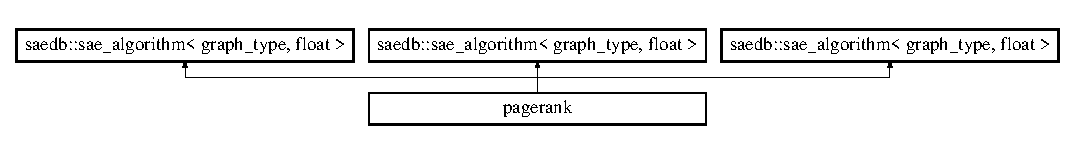
\includegraphics[height=1.441442cm]{d7/d39/classpagerank}
\end{center}
\end{figure}
\subsection*{Public Member Functions}
\begin{DoxyCompactItemize}
\item 
\hyperlink{namespacesaedb_adf5ad13c09a48fb2f42f8e7348ea3ac3}{edge\-\_\-dir\-\_\-type} \hyperlink{classpagerank_a6d6353f113e4e2035c530a1e731e5a04}{gather\-\_\-edges} (\hyperlink{classsaedb_1_1sae__algorithm_a190f07adbc04f0188ad09b50dbe93a33}{icontext\-\_\-type} \&context, const \hyperlink{classsaedb_1_1sae__algorithm_ae26abf349aed2b0c9f82e1396b78561a}{vertex\-\_\-type} \&vertex) const 
\item 
float \hyperlink{classpagerank_a2538fd5fbef7bf5032ace5a9427079ca}{gather} (\hyperlink{classsaedb_1_1sae__algorithm_a190f07adbc04f0188ad09b50dbe93a33}{icontext\-\_\-type} \&context, const \hyperlink{classsaedb_1_1sae__algorithm_ae26abf349aed2b0c9f82e1396b78561a}{vertex\-\_\-type} \&vertex, \hyperlink{classsaedb_1_1sae__algorithm_aaebb1836596e0efad3d694a5b829871f}{edge\-\_\-type} \&edge)
\item 
void \hyperlink{classpagerank_aad9830119d9cdf6099749c97c707cb79}{apply} (\hyperlink{classsaedb_1_1sae__algorithm_a190f07adbc04f0188ad09b50dbe93a33}{icontext\-\_\-type} \&context, \hyperlink{classsaedb_1_1sae__algorithm_ae26abf349aed2b0c9f82e1396b78561a}{vertex\-\_\-type} \&vertex, const \hyperlink{classsaedb_1_1sae__algorithm_a4c57e65dd3987f19d5d90bf394c8f2f8}{gather\-\_\-type} \&total)
\item 
\hyperlink{namespacesaedb_adf5ad13c09a48fb2f42f8e7348ea3ac3}{edge\-\_\-dir\-\_\-type} \hyperlink{classpagerank_a6cd84868333a4481a4d824bff82f2649}{scatter\-\_\-edges} (\hyperlink{classsaedb_1_1sae__algorithm_a190f07adbc04f0188ad09b50dbe93a33}{icontext\-\_\-type} \&context, const vertex)
\item 
void \hyperlink{classpagerank_a6216a1bceaf95e35325a0e6d70af35dd}{scatter} (\hyperlink{classsaedb_1_1sae__algorithm_a190f07adbc04f0188ad09b50dbe93a33}{icontext\-\_\-type} \&context, const \hyperlink{classsaedb_1_1sae__algorithm_ae26abf349aed2b0c9f82e1396b78561a}{vertex\-\_\-type} \&vertex, \hyperlink{classsaedb_1_1sae__algorithm_aaebb1836596e0efad3d694a5b829871f}{edge\-\_\-type} \&edge) const 
\item 
\hyperlink{namespacesaedb_adf5ad13c09a48fb2f42f8e7348ea3ac3}{edge\-\_\-dir\-\_\-type} \hyperlink{classpagerank_a6d6353f113e4e2035c530a1e731e5a04}{gather\-\_\-edges} (\hyperlink{classsaedb_1_1sae__algorithm_a190f07adbc04f0188ad09b50dbe93a33}{icontext\-\_\-type} \&context, const \hyperlink{classsaedb_1_1sae__algorithm_ae26abf349aed2b0c9f82e1396b78561a}{vertex\-\_\-type} \&vertex) const 
\item 
float \hyperlink{classpagerank_a2538fd5fbef7bf5032ace5a9427079ca}{gather} (\hyperlink{classsaedb_1_1sae__algorithm_a190f07adbc04f0188ad09b50dbe93a33}{icontext\-\_\-type} \&context, const \hyperlink{classsaedb_1_1sae__algorithm_ae26abf349aed2b0c9f82e1396b78561a}{vertex\-\_\-type} \&vertex, \hyperlink{classsaedb_1_1sae__algorithm_aaebb1836596e0efad3d694a5b829871f}{edge\-\_\-type} \&edge)
\item 
void \hyperlink{classpagerank_aad9830119d9cdf6099749c97c707cb79}{apply} (\hyperlink{classsaedb_1_1sae__algorithm_a190f07adbc04f0188ad09b50dbe93a33}{icontext\-\_\-type} \&context, \hyperlink{classsaedb_1_1sae__algorithm_ae26abf349aed2b0c9f82e1396b78561a}{vertex\-\_\-type} \&vertex, const \hyperlink{classsaedb_1_1sae__algorithm_a4c57e65dd3987f19d5d90bf394c8f2f8}{gather\-\_\-type} \&total)
\item 
\hyperlink{namespacesaedb_adf5ad13c09a48fb2f42f8e7348ea3ac3}{edge\-\_\-dir\-\_\-type} \hyperlink{classpagerank_a6cd84868333a4481a4d824bff82f2649}{scatter\-\_\-edges} (\hyperlink{classsaedb_1_1sae__algorithm_a190f07adbc04f0188ad09b50dbe93a33}{icontext\-\_\-type} \&context, const vertex)
\item 
void \hyperlink{classpagerank_a6216a1bceaf95e35325a0e6d70af35dd}{scatter} (\hyperlink{classsaedb_1_1sae__algorithm_a190f07adbc04f0188ad09b50dbe93a33}{icontext\-\_\-type} \&context, const \hyperlink{classsaedb_1_1sae__algorithm_ae26abf349aed2b0c9f82e1396b78561a}{vertex\-\_\-type} \&vertex, \hyperlink{classsaedb_1_1sae__algorithm_aaebb1836596e0efad3d694a5b829871f}{edge\-\_\-type} \&edge) const 
\item 
float \hyperlink{classpagerank_af1c6b5a1959b6667fb3adf6899d15964}{gather} (\hyperlink{classsaedb_1_1sae__algorithm_a190f07adbc04f0188ad09b50dbe93a33}{icontext\-\_\-type} \&context, const \hyperlink{classsaedb_1_1sae__algorithm_ae26abf349aed2b0c9f82e1396b78561a}{vertex\-\_\-type} \&vertex, \hyperlink{classsaedb_1_1sae__algorithm_aaebb1836596e0efad3d694a5b829871f}{edge\-\_\-type} \&edge) const 
\item 
void \hyperlink{classpagerank_aad9830119d9cdf6099749c97c707cb79}{apply} (\hyperlink{classsaedb_1_1sae__algorithm_a190f07adbc04f0188ad09b50dbe93a33}{icontext\-\_\-type} \&context, \hyperlink{classsaedb_1_1sae__algorithm_ae26abf349aed2b0c9f82e1396b78561a}{vertex\-\_\-type} \&vertex, const \hyperlink{classsaedb_1_1sae__algorithm_a4c57e65dd3987f19d5d90bf394c8f2f8}{gather\-\_\-type} \&total)
\item 
\hyperlink{namespacesaedb_adf5ad13c09a48fb2f42f8e7348ea3ac3}{edge\-\_\-dir\-\_\-type} \hyperlink{classpagerank_a518dd8b8877a509420ed834d8dbd129b}{scatter\-\_\-edges} (\hyperlink{classsaedb_1_1sae__algorithm_a190f07adbc04f0188ad09b50dbe93a33}{icontext\-\_\-type} \&context, const \hyperlink{classsaedb_1_1sae__algorithm_ae26abf349aed2b0c9f82e1396b78561a}{vertex\-\_\-type} \&vertex) const 
\item 
void \hyperlink{classpagerank_a6216a1bceaf95e35325a0e6d70af35dd}{scatter} (\hyperlink{classsaedb_1_1sae__algorithm_a190f07adbc04f0188ad09b50dbe93a33}{icontext\-\_\-type} \&context, const \hyperlink{classsaedb_1_1sae__algorithm_ae26abf349aed2b0c9f82e1396b78561a}{vertex\-\_\-type} \&vertex, \hyperlink{classsaedb_1_1sae__algorithm_aaebb1836596e0efad3d694a5b829871f}{edge\-\_\-type} \&edge) const 
\end{DoxyCompactItemize}
\subsection*{Additional Inherited Members}


\subsection{Detailed Description}


Definition at line 10 of file kmeans.\-cpp.



\subsection{Member Function Documentation}
\hypertarget{classpagerank_aad9830119d9cdf6099749c97c707cb79}{\index{pagerank@{pagerank}!apply@{apply}}
\index{apply@{apply}!pagerank@{pagerank}}
\subsubsection[{apply}]{\setlength{\rightskip}{0pt plus 5cm}void pagerank\-::apply (
\begin{DoxyParamCaption}
\item[{{\bf icontext\-\_\-type} \&}]{context, }
\item[{{\bf vertex\-\_\-type} \&}]{vertex, }
\item[{const {\bf gather\-\_\-type} \&}]{total}
\end{DoxyParamCaption}
)\hspace{0.3cm}{\ttfamily [inline]}, {\ttfamily [virtual]}}}\label{d7/d39/classpagerank_aad9830119d9cdf6099749c97c707cb79}


Implements \hyperlink{classsaedb_1_1sae__algorithm_a25fcc38700d5209fb2dcc81771253033}{saedb\-::sae\-\_\-algorithm$<$ graph\-\_\-type, float $>$}.



Definition at line 23 of file pagerank.\-cpp.

\hypertarget{classpagerank_aad9830119d9cdf6099749c97c707cb79}{\index{pagerank@{pagerank}!apply@{apply}}
\index{apply@{apply}!pagerank@{pagerank}}
\subsubsection[{apply}]{\setlength{\rightskip}{0pt plus 5cm}void pagerank\-::apply (
\begin{DoxyParamCaption}
\item[{{\bf icontext\-\_\-type} \&}]{context, }
\item[{{\bf vertex\-\_\-type} \&}]{vertex, }
\item[{const {\bf gather\-\_\-type} \&}]{total}
\end{DoxyParamCaption}
)\hspace{0.3cm}{\ttfamily [inline]}, {\ttfamily [virtual]}}}\label{d7/d39/classpagerank_aad9830119d9cdf6099749c97c707cb79}


Implements \hyperlink{classsaedb_1_1sae__algorithm_a25fcc38700d5209fb2dcc81771253033}{saedb\-::sae\-\_\-algorithm$<$ graph\-\_\-type, float $>$}.



Definition at line 25 of file pagerank.\-cpp.

\hypertarget{classpagerank_aad9830119d9cdf6099749c97c707cb79}{\index{pagerank@{pagerank}!apply@{apply}}
\index{apply@{apply}!pagerank@{pagerank}}
\subsubsection[{apply}]{\setlength{\rightskip}{0pt plus 5cm}void pagerank\-::apply (
\begin{DoxyParamCaption}
\item[{{\bf icontext\-\_\-type} \&}]{context, }
\item[{{\bf vertex\-\_\-type} \&}]{vertex, }
\item[{const {\bf gather\-\_\-type} \&}]{total}
\end{DoxyParamCaption}
)\hspace{0.3cm}{\ttfamily [inline]}, {\ttfamily [virtual]}}}\label{d7/d39/classpagerank_aad9830119d9cdf6099749c97c707cb79}


Implements \hyperlink{classsaedb_1_1sae__algorithm_a25fcc38700d5209fb2dcc81771253033}{saedb\-::sae\-\_\-algorithm$<$ graph\-\_\-type, float $>$}.



Definition at line 25 of file kmeans.\-cpp.

\hypertarget{classpagerank_af1c6b5a1959b6667fb3adf6899d15964}{\index{pagerank@{pagerank}!gather@{gather}}
\index{gather@{gather}!pagerank@{pagerank}}
\subsubsection[{gather}]{\setlength{\rightskip}{0pt plus 5cm}float pagerank\-::gather (
\begin{DoxyParamCaption}
\item[{{\bf icontext\-\_\-type} \&}]{context, }
\item[{const {\bf vertex\-\_\-type} \&}]{vertex, }
\item[{{\bf edge\-\_\-type} \&}]{edge}
\end{DoxyParamCaption}
) const\hspace{0.3cm}{\ttfamily [inline]}, {\ttfamily [virtual]}}}\label{d7/d39/classpagerank_af1c6b5a1959b6667fb3adf6899d15964}


Reimplemented from \hyperlink{classsaedb_1_1sae__algorithm_aef9f7edc10a5e76234157db8c9c8c2bb}{saedb\-::sae\-\_\-algorithm$<$ graph\-\_\-type, float $>$}.



Definition at line 17 of file pagerank.\-cpp.

\hypertarget{classpagerank_a2538fd5fbef7bf5032ace5a9427079ca}{\index{pagerank@{pagerank}!gather@{gather}}
\index{gather@{gather}!pagerank@{pagerank}}
\subsubsection[{gather}]{\setlength{\rightskip}{0pt plus 5cm}float pagerank\-::gather (
\begin{DoxyParamCaption}
\item[{{\bf icontext\-\_\-type} \&}]{context, }
\item[{const {\bf vertex\-\_\-type} \&}]{vertex, }
\item[{{\bf edge\-\_\-type} \&}]{edge}
\end{DoxyParamCaption}
)\hspace{0.3cm}{\ttfamily [inline]}}}\label{d7/d39/classpagerank_a2538fd5fbef7bf5032ace5a9427079ca}


Definition at line 18 of file kmeans.\-cpp.

\hypertarget{classpagerank_a2538fd5fbef7bf5032ace5a9427079ca}{\index{pagerank@{pagerank}!gather@{gather}}
\index{gather@{gather}!pagerank@{pagerank}}
\subsubsection[{gather}]{\setlength{\rightskip}{0pt plus 5cm}float pagerank\-::gather (
\begin{DoxyParamCaption}
\item[{{\bf icontext\-\_\-type} \&}]{context, }
\item[{const {\bf vertex\-\_\-type} \&}]{vertex, }
\item[{{\bf edge\-\_\-type} \&}]{edge}
\end{DoxyParamCaption}
)\hspace{0.3cm}{\ttfamily [inline]}}}\label{d7/d39/classpagerank_a2538fd5fbef7bf5032ace5a9427079ca}


Definition at line 18 of file pagerank.\-cpp.

\hypertarget{classpagerank_a6d6353f113e4e2035c530a1e731e5a04}{\index{pagerank@{pagerank}!gather\-\_\-edges@{gather\-\_\-edges}}
\index{gather\-\_\-edges@{gather\-\_\-edges}!pagerank@{pagerank}}
\subsubsection[{gather\-\_\-edges}]{\setlength{\rightskip}{0pt plus 5cm}{\bf edge\-\_\-dir\-\_\-type} pagerank\-::gather\-\_\-edges (
\begin{DoxyParamCaption}
\item[{{\bf icontext\-\_\-type} \&}]{context, }
\item[{const {\bf vertex\-\_\-type} \&}]{vertex}
\end{DoxyParamCaption}
) const\hspace{0.3cm}{\ttfamily [inline]}, {\ttfamily [virtual]}}}\label{d7/d39/classpagerank_a6d6353f113e4e2035c530a1e731e5a04}


Reimplemented from \hyperlink{classsaedb_1_1sae__algorithm_aa2930d50f01ae01c12639a19e517329f}{saedb\-::sae\-\_\-algorithm$<$ graph\-\_\-type, float $>$}.



Definition at line 13 of file kmeans.\-cpp.

\hypertarget{classpagerank_a6d6353f113e4e2035c530a1e731e5a04}{\index{pagerank@{pagerank}!gather\-\_\-edges@{gather\-\_\-edges}}
\index{gather\-\_\-edges@{gather\-\_\-edges}!pagerank@{pagerank}}
\subsubsection[{gather\-\_\-edges}]{\setlength{\rightskip}{0pt plus 5cm}{\bf edge\-\_\-dir\-\_\-type} pagerank\-::gather\-\_\-edges (
\begin{DoxyParamCaption}
\item[{{\bf icontext\-\_\-type} \&}]{context, }
\item[{const {\bf vertex\-\_\-type} \&}]{vertex}
\end{DoxyParamCaption}
) const\hspace{0.3cm}{\ttfamily [inline]}, {\ttfamily [virtual]}}}\label{d7/d39/classpagerank_a6d6353f113e4e2035c530a1e731e5a04}


Reimplemented from \hyperlink{classsaedb_1_1sae__algorithm_aa2930d50f01ae01c12639a19e517329f}{saedb\-::sae\-\_\-algorithm$<$ graph\-\_\-type, float $>$}.



Definition at line 13 of file pagerank.\-cpp.

\hypertarget{classpagerank_a6216a1bceaf95e35325a0e6d70af35dd}{\index{pagerank@{pagerank}!scatter@{scatter}}
\index{scatter@{scatter}!pagerank@{pagerank}}
\subsubsection[{scatter}]{\setlength{\rightskip}{0pt plus 5cm}void pagerank\-::scatter (
\begin{DoxyParamCaption}
\item[{{\bf icontext\-\_\-type} \&}]{context, }
\item[{const {\bf vertex\-\_\-type} \&}]{vertex, }
\item[{{\bf edge\-\_\-type} \&}]{edge}
\end{DoxyParamCaption}
) const\hspace{0.3cm}{\ttfamily [inline]}, {\ttfamily [virtual]}}}\label{d7/d39/classpagerank_a6216a1bceaf95e35325a0e6d70af35dd}


Reimplemented from \hyperlink{classsaedb_1_1sae__algorithm_a584008f538972457cf702cc8cac474bf}{saedb\-::sae\-\_\-algorithm$<$ graph\-\_\-type, float $>$}.



Definition at line 34 of file pagerank.\-cpp.

\hypertarget{classpagerank_a6216a1bceaf95e35325a0e6d70af35dd}{\index{pagerank@{pagerank}!scatter@{scatter}}
\index{scatter@{scatter}!pagerank@{pagerank}}
\subsubsection[{scatter}]{\setlength{\rightskip}{0pt plus 5cm}void pagerank\-::scatter (
\begin{DoxyParamCaption}
\item[{{\bf icontext\-\_\-type} \&}]{context, }
\item[{const {\bf vertex\-\_\-type} \&}]{vertex, }
\item[{{\bf edge\-\_\-type} \&}]{edge}
\end{DoxyParamCaption}
) const\hspace{0.3cm}{\ttfamily [inline]}, {\ttfamily [virtual]}}}\label{d7/d39/classpagerank_a6216a1bceaf95e35325a0e6d70af35dd}


Reimplemented from \hyperlink{classsaedb_1_1sae__algorithm_a584008f538972457cf702cc8cac474bf}{saedb\-::sae\-\_\-algorithm$<$ graph\-\_\-type, float $>$}.



Definition at line 34 of file kmeans.\-cpp.

\hypertarget{classpagerank_a6216a1bceaf95e35325a0e6d70af35dd}{\index{pagerank@{pagerank}!scatter@{scatter}}
\index{scatter@{scatter}!pagerank@{pagerank}}
\subsubsection[{scatter}]{\setlength{\rightskip}{0pt plus 5cm}void pagerank\-::scatter (
\begin{DoxyParamCaption}
\item[{{\bf icontext\-\_\-type} \&}]{context, }
\item[{const {\bf vertex\-\_\-type} \&}]{vertex, }
\item[{{\bf edge\-\_\-type} \&}]{edge}
\end{DoxyParamCaption}
) const\hspace{0.3cm}{\ttfamily [inline]}, {\ttfamily [virtual]}}}\label{d7/d39/classpagerank_a6216a1bceaf95e35325a0e6d70af35dd}


Reimplemented from \hyperlink{classsaedb_1_1sae__algorithm_a584008f538972457cf702cc8cac474bf}{saedb\-::sae\-\_\-algorithm$<$ graph\-\_\-type, float $>$}.



Definition at line 34 of file pagerank.\-cpp.

\hypertarget{classpagerank_a518dd8b8877a509420ed834d8dbd129b}{\index{pagerank@{pagerank}!scatter\-\_\-edges@{scatter\-\_\-edges}}
\index{scatter\-\_\-edges@{scatter\-\_\-edges}!pagerank@{pagerank}}
\subsubsection[{scatter\-\_\-edges}]{\setlength{\rightskip}{0pt plus 5cm}{\bf edge\-\_\-dir\-\_\-type} pagerank\-::scatter\-\_\-edges (
\begin{DoxyParamCaption}
\item[{{\bf icontext\-\_\-type} \&}]{context, }
\item[{const {\bf vertex\-\_\-type} \&}]{vertex}
\end{DoxyParamCaption}
) const\hspace{0.3cm}{\ttfamily [inline]}, {\ttfamily [virtual]}}}\label{d7/d39/classpagerank_a518dd8b8877a509420ed834d8dbd129b}


Reimplemented from \hyperlink{classsaedb_1_1sae__algorithm_adfc160930509d2259cb98f96a80d1232}{saedb\-::sae\-\_\-algorithm$<$ graph\-\_\-type, float $>$}.



Definition at line 29 of file pagerank.\-cpp.

\hypertarget{classpagerank_a6cd84868333a4481a4d824bff82f2649}{\index{pagerank@{pagerank}!scatter\-\_\-edges@{scatter\-\_\-edges}}
\index{scatter\-\_\-edges@{scatter\-\_\-edges}!pagerank@{pagerank}}
\subsubsection[{scatter\-\_\-edges}]{\setlength{\rightskip}{0pt plus 5cm}{\bf edge\-\_\-dir\-\_\-type} pagerank\-::scatter\-\_\-edges (
\begin{DoxyParamCaption}
\item[{{\bf icontext\-\_\-type} \&}]{context, }
\item[{const vertex}]{}
\end{DoxyParamCaption}
)\hspace{0.3cm}{\ttfamily [inline]}}}\label{d7/d39/classpagerank_a6cd84868333a4481a4d824bff82f2649}


Definition at line 30 of file pagerank.\-cpp.

\hypertarget{classpagerank_a6cd84868333a4481a4d824bff82f2649}{\index{pagerank@{pagerank}!scatter\-\_\-edges@{scatter\-\_\-edges}}
\index{scatter\-\_\-edges@{scatter\-\_\-edges}!pagerank@{pagerank}}
\subsubsection[{scatter\-\_\-edges}]{\setlength{\rightskip}{0pt plus 5cm}{\bf edge\-\_\-dir\-\_\-type} pagerank\-::scatter\-\_\-edges (
\begin{DoxyParamCaption}
\item[{{\bf icontext\-\_\-type} \&}]{context, }
\item[{const vertex}]{}
\end{DoxyParamCaption}
)\hspace{0.3cm}{\ttfamily [inline]}}}\label{d7/d39/classpagerank_a6cd84868333a4481a4d824bff82f2649}


Definition at line 30 of file kmeans.\-cpp.



The documentation for this class was generated from the following files\-:\begin{DoxyCompactItemize}
\item 
src/app/basic/clustering/\hyperlink{kmeans_8cpp}{kmeans.\-cpp}\item 
src/app/basic/pagerank/\hyperlink{basic_2pagerank_2pagerank_8cpp}{pagerank.\-cpp}\item 
src/app/demo/pagerank/\hyperlink{demo_2pagerank_2pagerank_8cpp}{pagerank.\-cpp}\end{DoxyCompactItemize}

\hypertarget{classsaedb_1_1sae__algorithm}{\section{saedb\-:\-:sae\-\_\-algorithm$<$ Graph, Gather\-Type, Message\-Type $>$ Class Template Reference}
\label{d0/d9f/classsaedb_1_1sae__algorithm}\index{saedb\-::sae\-\_\-algorithm$<$ Graph, Gather\-Type, Message\-Type $>$@{saedb\-::sae\-\_\-algorithm$<$ Graph, Gather\-Type, Message\-Type $>$}}
}


{\ttfamily \#include $<$vertex\-\_\-program.\-hpp$>$}

\subsection*{Public Types}
\begin{DoxyCompactItemize}
\item 
typedef Graph\-::vertex\-\_\-data\-\_\-type \hyperlink{classsaedb_1_1sae__algorithm_a709b55d6063cfd2c5f0dcdb17d6d5258}{vertex\-\_\-data\-\_\-type}
\item 
typedef Graph\-::edge\-\_\-data\-\_\-type \hyperlink{classsaedb_1_1sae__algorithm_a1d3acc631f0a3e22c830c91dcf104c8a}{edge\-\_\-data\-\_\-type}
\item 
typedef Gather\-Type \hyperlink{classsaedb_1_1sae__algorithm_a4c57e65dd3987f19d5d90bf394c8f2f8}{gather\-\_\-type}
\item 
typedef Graph \hyperlink{classsaedb_1_1sae__algorithm_a87749c5b779e21642c2928b746556540}{graph\-\_\-type}
\item 
typedef Message\-Type \hyperlink{classsaedb_1_1sae__algorithm_a757eb6dffc652f91f2c10a24f6596156}{message\-\_\-type}
\item 
typedef \hyperlink{classsaedb_1_1sae__graph_a2f9a7bf2db556689f1cd9de9562ff41f}{graph\-\_\-type\-::vertex\-\_\-id\-\_\-type} \hyperlink{classsaedb_1_1sae__algorithm_a943e87163aee5f148d7a7c68be72b123}{vertex\-\_\-id\-\_\-type}
\item 
typedef \hyperlink{structsaedb_1_1sae__graph_1_1vertex__type}{graph\-\_\-type\-::vertex\-\_\-type} \hyperlink{classsaedb_1_1sae__algorithm_ae26abf349aed2b0c9f82e1396b78561a}{vertex\-\_\-type}
\item 
typedef \hyperlink{classsaedb_1_1sae__graph_1_1edge__type}{graph\-\_\-type\-::edge\-\_\-type} \hyperlink{classsaedb_1_1sae__algorithm_aaebb1836596e0efad3d694a5b829871f}{edge\-\_\-type}
\item 
typedef \hyperlink{namespacesaedb_adf5ad13c09a48fb2f42f8e7348ea3ac3}{saedb\-::edge\-\_\-dir\-\_\-type} \hyperlink{classsaedb_1_1sae__algorithm_a0918d4a10cf91f715a686560b5b95b03}{edge\-\_\-dir\-\_\-type}
\item 
typedef \hyperlink{classsaedb_1_1icontext}{icontext}$<$ \hyperlink{classsaedb_1_1sae__algorithm_a87749c5b779e21642c2928b746556540}{graph\-\_\-type}, \\*
\hyperlink{classsaedb_1_1sae__algorithm_a4c57e65dd3987f19d5d90bf394c8f2f8}{gather\-\_\-type}, \hyperlink{classsaedb_1_1sae__algorithm_a757eb6dffc652f91f2c10a24f6596156}{message\-\_\-type} $>$ \hyperlink{classsaedb_1_1sae__algorithm_a190f07adbc04f0188ad09b50dbe93a33}{icontext\-\_\-type}
\end{DoxyCompactItemize}
\subsection*{Public Member Functions}
\begin{DoxyCompactItemize}
\item 
virtual \hyperlink{classsaedb_1_1sae__algorithm_ae67be2fe37126b9ab28b1be43a6b1e96}{$\sim$sae\-\_\-algorithm} ()
\item 
virtual void \hyperlink{classsaedb_1_1sae__algorithm_aae58b92247a316b2734704e24ee20700}{init} (\hyperlink{classsaedb_1_1sae__algorithm_a190f07adbc04f0188ad09b50dbe93a33}{icontext\-\_\-type} \&\hyperlink{classsaedb_1_1context}{context}, const \hyperlink{classsaedb_1_1sae__algorithm_ae26abf349aed2b0c9f82e1396b78561a}{vertex\-\_\-type} \&vertex)
\item 
virtual \hyperlink{namespacesaedb_adf5ad13c09a48fb2f42f8e7348ea3ac3}{edge\-\_\-dir\-\_\-type} \hyperlink{classsaedb_1_1sae__algorithm_aa2930d50f01ae01c12639a19e517329f}{gather\-\_\-edges} (\hyperlink{classsaedb_1_1sae__algorithm_a190f07adbc04f0188ad09b50dbe93a33}{icontext\-\_\-type} \&\hyperlink{classsaedb_1_1context}{context}, const \hyperlink{classsaedb_1_1sae__algorithm_ae26abf349aed2b0c9f82e1396b78561a}{vertex\-\_\-type} \&vertex) const 
\item 
virtual \hyperlink{classsaedb_1_1sae__algorithm_a4c57e65dd3987f19d5d90bf394c8f2f8}{gather\-\_\-type} \hyperlink{classsaedb_1_1sae__algorithm_aef9f7edc10a5e76234157db8c9c8c2bb}{gather} (\hyperlink{classsaedb_1_1sae__algorithm_a190f07adbc04f0188ad09b50dbe93a33}{icontext\-\_\-type} \&\hyperlink{classsaedb_1_1context}{context}, const \hyperlink{classsaedb_1_1sae__algorithm_ae26abf349aed2b0c9f82e1396b78561a}{vertex\-\_\-type} \&vertex, \hyperlink{classsaedb_1_1sae__algorithm_aaebb1836596e0efad3d694a5b829871f}{edge\-\_\-type} \&edge) const 
\item 
virtual void \hyperlink{classsaedb_1_1sae__algorithm_a25fcc38700d5209fb2dcc81771253033}{apply} (\hyperlink{classsaedb_1_1sae__algorithm_a190f07adbc04f0188ad09b50dbe93a33}{icontext\-\_\-type} \&\hyperlink{classsaedb_1_1context}{context}, \hyperlink{classsaedb_1_1sae__algorithm_ae26abf349aed2b0c9f82e1396b78561a}{vertex\-\_\-type} \&vertex, const \hyperlink{classsaedb_1_1sae__algorithm_a4c57e65dd3987f19d5d90bf394c8f2f8}{gather\-\_\-type} \&total)=0
\item 
virtual \hyperlink{namespacesaedb_adf5ad13c09a48fb2f42f8e7348ea3ac3}{edge\-\_\-dir\-\_\-type} \hyperlink{classsaedb_1_1sae__algorithm_adfc160930509d2259cb98f96a80d1232}{scatter\-\_\-edges} (\hyperlink{classsaedb_1_1sae__algorithm_a190f07adbc04f0188ad09b50dbe93a33}{icontext\-\_\-type} \&\hyperlink{classsaedb_1_1context}{context}, const \hyperlink{classsaedb_1_1sae__algorithm_ae26abf349aed2b0c9f82e1396b78561a}{vertex\-\_\-type} \&vertex) const 
\item 
virtual void \hyperlink{classsaedb_1_1sae__algorithm_a584008f538972457cf702cc8cac474bf}{scatter} (\hyperlink{classsaedb_1_1sae__algorithm_a190f07adbc04f0188ad09b50dbe93a33}{icontext\-\_\-type} \&\hyperlink{classsaedb_1_1context}{context}, const \hyperlink{classsaedb_1_1sae__algorithm_ae26abf349aed2b0c9f82e1396b78561a}{vertex\-\_\-type} \&vertex, \hyperlink{classsaedb_1_1sae__algorithm_aaebb1836596e0efad3d694a5b829871f}{edge\-\_\-type} \&edge) const 
\end{DoxyCompactItemize}


\subsection{Detailed Description}
\subsubsection*{template$<$typename Graph, typename Gather\-Type, typename Message\-Type = float$>$class saedb\-::sae\-\_\-algorithm$<$ Graph, Gather\-Type, Message\-Type $>$}



Definition at line 12 of file vertex\-\_\-program.\-hpp.



\subsection{Member Typedef Documentation}
\hypertarget{classsaedb_1_1sae__algorithm_a1d3acc631f0a3e22c830c91dcf104c8a}{\index{saedb\-::sae\-\_\-algorithm@{saedb\-::sae\-\_\-algorithm}!edge\-\_\-data\-\_\-type@{edge\-\_\-data\-\_\-type}}
\index{edge\-\_\-data\-\_\-type@{edge\-\_\-data\-\_\-type}!saedb::sae_algorithm@{saedb\-::sae\-\_\-algorithm}}
\subsubsection[{edge\-\_\-data\-\_\-type}]{\setlength{\rightskip}{0pt plus 5cm}template$<$typename Graph, typename Gather\-Type, typename Message\-Type = float$>$ typedef Graph\-::edge\-\_\-data\-\_\-type {\bf saedb\-::sae\-\_\-algorithm}$<$ Graph, Gather\-Type, Message\-Type $>$\-::{\bf edge\-\_\-data\-\_\-type}}}\label{d0/d9f/classsaedb_1_1sae__algorithm_a1d3acc631f0a3e22c830c91dcf104c8a}


Definition at line 16 of file vertex\-\_\-program.\-hpp.

\hypertarget{classsaedb_1_1sae__algorithm_a0918d4a10cf91f715a686560b5b95b03}{\index{saedb\-::sae\-\_\-algorithm@{saedb\-::sae\-\_\-algorithm}!edge\-\_\-dir\-\_\-type@{edge\-\_\-dir\-\_\-type}}
\index{edge\-\_\-dir\-\_\-type@{edge\-\_\-dir\-\_\-type}!saedb::sae_algorithm@{saedb\-::sae\-\_\-algorithm}}
\subsubsection[{edge\-\_\-dir\-\_\-type}]{\setlength{\rightskip}{0pt plus 5cm}template$<$typename Graph, typename Gather\-Type, typename Message\-Type = float$>$ typedef {\bf saedb\-::edge\-\_\-dir\-\_\-type} {\bf saedb\-::sae\-\_\-algorithm}$<$ Graph, Gather\-Type, Message\-Type $>$\-::{\bf edge\-\_\-dir\-\_\-type}}}\label{d0/d9f/classsaedb_1_1sae__algorithm_a0918d4a10cf91f715a686560b5b95b03}


Definition at line 23 of file vertex\-\_\-program.\-hpp.

\hypertarget{classsaedb_1_1sae__algorithm_aaebb1836596e0efad3d694a5b829871f}{\index{saedb\-::sae\-\_\-algorithm@{saedb\-::sae\-\_\-algorithm}!edge\-\_\-type@{edge\-\_\-type}}
\index{edge\-\_\-type@{edge\-\_\-type}!saedb::sae_algorithm@{saedb\-::sae\-\_\-algorithm}}
\subsubsection[{edge\-\_\-type}]{\setlength{\rightskip}{0pt plus 5cm}template$<$typename Graph, typename Gather\-Type, typename Message\-Type = float$>$ typedef {\bf graph\-\_\-type\-::edge\-\_\-type} {\bf saedb\-::sae\-\_\-algorithm}$<$ Graph, Gather\-Type, Message\-Type $>$\-::{\bf edge\-\_\-type}}}\label{d0/d9f/classsaedb_1_1sae__algorithm_aaebb1836596e0efad3d694a5b829871f}


Definition at line 22 of file vertex\-\_\-program.\-hpp.

\hypertarget{classsaedb_1_1sae__algorithm_a4c57e65dd3987f19d5d90bf394c8f2f8}{\index{saedb\-::sae\-\_\-algorithm@{saedb\-::sae\-\_\-algorithm}!gather\-\_\-type@{gather\-\_\-type}}
\index{gather\-\_\-type@{gather\-\_\-type}!saedb::sae_algorithm@{saedb\-::sae\-\_\-algorithm}}
\subsubsection[{gather\-\_\-type}]{\setlength{\rightskip}{0pt plus 5cm}template$<$typename Graph, typename Gather\-Type, typename Message\-Type = float$>$ typedef Gather\-Type {\bf saedb\-::sae\-\_\-algorithm}$<$ Graph, Gather\-Type, Message\-Type $>$\-::{\bf gather\-\_\-type}}}\label{d0/d9f/classsaedb_1_1sae__algorithm_a4c57e65dd3987f19d5d90bf394c8f2f8}


Definition at line 17 of file vertex\-\_\-program.\-hpp.

\hypertarget{classsaedb_1_1sae__algorithm_a87749c5b779e21642c2928b746556540}{\index{saedb\-::sae\-\_\-algorithm@{saedb\-::sae\-\_\-algorithm}!graph\-\_\-type@{graph\-\_\-type}}
\index{graph\-\_\-type@{graph\-\_\-type}!saedb::sae_algorithm@{saedb\-::sae\-\_\-algorithm}}
\subsubsection[{graph\-\_\-type}]{\setlength{\rightskip}{0pt plus 5cm}template$<$typename Graph, typename Gather\-Type, typename Message\-Type = float$>$ typedef Graph {\bf saedb\-::sae\-\_\-algorithm}$<$ Graph, Gather\-Type, Message\-Type $>$\-::{\bf graph\-\_\-type}}}\label{d0/d9f/classsaedb_1_1sae__algorithm_a87749c5b779e21642c2928b746556540}


Definition at line 18 of file vertex\-\_\-program.\-hpp.

\hypertarget{classsaedb_1_1sae__algorithm_a190f07adbc04f0188ad09b50dbe93a33}{\index{saedb\-::sae\-\_\-algorithm@{saedb\-::sae\-\_\-algorithm}!icontext\-\_\-type@{icontext\-\_\-type}}
\index{icontext\-\_\-type@{icontext\-\_\-type}!saedb::sae_algorithm@{saedb\-::sae\-\_\-algorithm}}
\subsubsection[{icontext\-\_\-type}]{\setlength{\rightskip}{0pt plus 5cm}template$<$typename Graph, typename Gather\-Type, typename Message\-Type = float$>$ typedef {\bf icontext}$<${\bf graph\-\_\-type}, {\bf gather\-\_\-type}, {\bf message\-\_\-type}$>$ {\bf saedb\-::sae\-\_\-algorithm}$<$ Graph, Gather\-Type, Message\-Type $>$\-::{\bf icontext\-\_\-type}}}\label{d0/d9f/classsaedb_1_1sae__algorithm_a190f07adbc04f0188ad09b50dbe93a33}


Definition at line 24 of file vertex\-\_\-program.\-hpp.

\hypertarget{classsaedb_1_1sae__algorithm_a757eb6dffc652f91f2c10a24f6596156}{\index{saedb\-::sae\-\_\-algorithm@{saedb\-::sae\-\_\-algorithm}!message\-\_\-type@{message\-\_\-type}}
\index{message\-\_\-type@{message\-\_\-type}!saedb::sae_algorithm@{saedb\-::sae\-\_\-algorithm}}
\subsubsection[{message\-\_\-type}]{\setlength{\rightskip}{0pt plus 5cm}template$<$typename Graph, typename Gather\-Type, typename Message\-Type = float$>$ typedef Message\-Type {\bf saedb\-::sae\-\_\-algorithm}$<$ Graph, Gather\-Type, Message\-Type $>$\-::{\bf message\-\_\-type}}}\label{d0/d9f/classsaedb_1_1sae__algorithm_a757eb6dffc652f91f2c10a24f6596156}


Definition at line 19 of file vertex\-\_\-program.\-hpp.

\hypertarget{classsaedb_1_1sae__algorithm_a709b55d6063cfd2c5f0dcdb17d6d5258}{\index{saedb\-::sae\-\_\-algorithm@{saedb\-::sae\-\_\-algorithm}!vertex\-\_\-data\-\_\-type@{vertex\-\_\-data\-\_\-type}}
\index{vertex\-\_\-data\-\_\-type@{vertex\-\_\-data\-\_\-type}!saedb::sae_algorithm@{saedb\-::sae\-\_\-algorithm}}
\subsubsection[{vertex\-\_\-data\-\_\-type}]{\setlength{\rightskip}{0pt plus 5cm}template$<$typename Graph, typename Gather\-Type, typename Message\-Type = float$>$ typedef Graph\-::vertex\-\_\-data\-\_\-type {\bf saedb\-::sae\-\_\-algorithm}$<$ Graph, Gather\-Type, Message\-Type $>$\-::{\bf vertex\-\_\-data\-\_\-type}}}\label{d0/d9f/classsaedb_1_1sae__algorithm_a709b55d6063cfd2c5f0dcdb17d6d5258}


Definition at line 15 of file vertex\-\_\-program.\-hpp.

\hypertarget{classsaedb_1_1sae__algorithm_a943e87163aee5f148d7a7c68be72b123}{\index{saedb\-::sae\-\_\-algorithm@{saedb\-::sae\-\_\-algorithm}!vertex\-\_\-id\-\_\-type@{vertex\-\_\-id\-\_\-type}}
\index{vertex\-\_\-id\-\_\-type@{vertex\-\_\-id\-\_\-type}!saedb::sae_algorithm@{saedb\-::sae\-\_\-algorithm}}
\subsubsection[{vertex\-\_\-id\-\_\-type}]{\setlength{\rightskip}{0pt plus 5cm}template$<$typename Graph, typename Gather\-Type, typename Message\-Type = float$>$ typedef {\bf graph\-\_\-type\-::vertex\-\_\-id\-\_\-type} {\bf saedb\-::sae\-\_\-algorithm}$<$ Graph, Gather\-Type, Message\-Type $>$\-::{\bf vertex\-\_\-id\-\_\-type}}}\label{d0/d9f/classsaedb_1_1sae__algorithm_a943e87163aee5f148d7a7c68be72b123}


Definition at line 20 of file vertex\-\_\-program.\-hpp.

\hypertarget{classsaedb_1_1sae__algorithm_ae26abf349aed2b0c9f82e1396b78561a}{\index{saedb\-::sae\-\_\-algorithm@{saedb\-::sae\-\_\-algorithm}!vertex\-\_\-type@{vertex\-\_\-type}}
\index{vertex\-\_\-type@{vertex\-\_\-type}!saedb::sae_algorithm@{saedb\-::sae\-\_\-algorithm}}
\subsubsection[{vertex\-\_\-type}]{\setlength{\rightskip}{0pt plus 5cm}template$<$typename Graph, typename Gather\-Type, typename Message\-Type = float$>$ typedef {\bf graph\-\_\-type\-::vertex\-\_\-type} {\bf saedb\-::sae\-\_\-algorithm}$<$ Graph, Gather\-Type, Message\-Type $>$\-::{\bf vertex\-\_\-type}}}\label{d0/d9f/classsaedb_1_1sae__algorithm_ae26abf349aed2b0c9f82e1396b78561a}


Definition at line 21 of file vertex\-\_\-program.\-hpp.



\subsection{Constructor \& Destructor Documentation}
\hypertarget{classsaedb_1_1sae__algorithm_ae67be2fe37126b9ab28b1be43a6b1e96}{\index{saedb\-::sae\-\_\-algorithm@{saedb\-::sae\-\_\-algorithm}!$\sim$sae\-\_\-algorithm@{$\sim$sae\-\_\-algorithm}}
\index{$\sim$sae\-\_\-algorithm@{$\sim$sae\-\_\-algorithm}!saedb::sae_algorithm@{saedb\-::sae\-\_\-algorithm}}
\subsubsection[{$\sim$sae\-\_\-algorithm}]{\setlength{\rightskip}{0pt plus 5cm}template$<$typename Graph, typename Gather\-Type, typename Message\-Type = float$>$ virtual {\bf saedb\-::sae\-\_\-algorithm}$<$ Graph, Gather\-Type, Message\-Type $>$\-::$\sim${\bf sae\-\_\-algorithm} (
\begin{DoxyParamCaption}
{}
\end{DoxyParamCaption}
)\hspace{0.3cm}{\ttfamily [inline]}, {\ttfamily [virtual]}}}\label{d0/d9f/classsaedb_1_1sae__algorithm_ae67be2fe37126b9ab28b1be43a6b1e96}


Definition at line 26 of file vertex\-\_\-program.\-hpp.



\subsection{Member Function Documentation}
\hypertarget{classsaedb_1_1sae__algorithm_a25fcc38700d5209fb2dcc81771253033}{\index{saedb\-::sae\-\_\-algorithm@{saedb\-::sae\-\_\-algorithm}!apply@{apply}}
\index{apply@{apply}!saedb::sae_algorithm@{saedb\-::sae\-\_\-algorithm}}
\subsubsection[{apply}]{\setlength{\rightskip}{0pt plus 5cm}template$<$typename Graph, typename Gather\-Type, typename Message\-Type = float$>$ virtual void {\bf saedb\-::sae\-\_\-algorithm}$<$ Graph, Gather\-Type, Message\-Type $>$\-::apply (
\begin{DoxyParamCaption}
\item[{{\bf icontext\-\_\-type} \&}]{context, }
\item[{{\bf vertex\-\_\-type} \&}]{vertex, }
\item[{const {\bf gather\-\_\-type} \&}]{total}
\end{DoxyParamCaption}
)\hspace{0.3cm}{\ttfamily [pure virtual]}}}\label{d0/d9f/classsaedb_1_1sae__algorithm_a25fcc38700d5209fb2dcc81771253033}


Implemented in \hyperlink{classpagerank_aad9830119d9cdf6099749c97c707cb79}{pagerank}, \hyperlink{classpagerank_aad9830119d9cdf6099749c97c707cb79}{pagerank}, and \hyperlink{classpagerank_aad9830119d9cdf6099749c97c707cb79}{pagerank}.

\hypertarget{classsaedb_1_1sae__algorithm_aef9f7edc10a5e76234157db8c9c8c2bb}{\index{saedb\-::sae\-\_\-algorithm@{saedb\-::sae\-\_\-algorithm}!gather@{gather}}
\index{gather@{gather}!saedb::sae_algorithm@{saedb\-::sae\-\_\-algorithm}}
\subsubsection[{gather}]{\setlength{\rightskip}{0pt plus 5cm}template$<$typename Graph, typename Gather\-Type, typename Message\-Type = float$>$ virtual {\bf gather\-\_\-type} {\bf saedb\-::sae\-\_\-algorithm}$<$ Graph, Gather\-Type, Message\-Type $>$\-::gather (
\begin{DoxyParamCaption}
\item[{{\bf icontext\-\_\-type} \&}]{context, }
\item[{const {\bf vertex\-\_\-type} \&}]{vertex, }
\item[{{\bf edge\-\_\-type} \&}]{edge}
\end{DoxyParamCaption}
) const\hspace{0.3cm}{\ttfamily [inline]}, {\ttfamily [virtual]}}}\label{d0/d9f/classsaedb_1_1sae__algorithm_aef9f7edc10a5e76234157db8c9c8c2bb}


Reimplemented in \hyperlink{classpagerank_af1c6b5a1959b6667fb3adf6899d15964}{pagerank}.



Definition at line 36 of file vertex\-\_\-program.\-hpp.

\hypertarget{classsaedb_1_1sae__algorithm_aa2930d50f01ae01c12639a19e517329f}{\index{saedb\-::sae\-\_\-algorithm@{saedb\-::sae\-\_\-algorithm}!gather\-\_\-edges@{gather\-\_\-edges}}
\index{gather\-\_\-edges@{gather\-\_\-edges}!saedb::sae_algorithm@{saedb\-::sae\-\_\-algorithm}}
\subsubsection[{gather\-\_\-edges}]{\setlength{\rightskip}{0pt plus 5cm}template$<$typename Graph, typename Gather\-Type, typename Message\-Type = float$>$ virtual {\bf edge\-\_\-dir\-\_\-type} {\bf saedb\-::sae\-\_\-algorithm}$<$ Graph, Gather\-Type, Message\-Type $>$\-::gather\-\_\-edges (
\begin{DoxyParamCaption}
\item[{{\bf icontext\-\_\-type} \&}]{context, }
\item[{const {\bf vertex\-\_\-type} \&}]{vertex}
\end{DoxyParamCaption}
) const\hspace{0.3cm}{\ttfamily [inline]}, {\ttfamily [virtual]}}}\label{d0/d9f/classsaedb_1_1sae__algorithm_aa2930d50f01ae01c12639a19e517329f}


Reimplemented in \hyperlink{classpagerank_a6d6353f113e4e2035c530a1e731e5a04}{pagerank}, and \hyperlink{classpagerank_a6d6353f113e4e2035c530a1e731e5a04}{pagerank}.



Definition at line 31 of file vertex\-\_\-program.\-hpp.

\hypertarget{classsaedb_1_1sae__algorithm_aae58b92247a316b2734704e24ee20700}{\index{saedb\-::sae\-\_\-algorithm@{saedb\-::sae\-\_\-algorithm}!init@{init}}
\index{init@{init}!saedb::sae_algorithm@{saedb\-::sae\-\_\-algorithm}}
\subsubsection[{init}]{\setlength{\rightskip}{0pt plus 5cm}template$<$typename Graph, typename Gather\-Type, typename Message\-Type = float$>$ virtual void {\bf saedb\-::sae\-\_\-algorithm}$<$ Graph, Gather\-Type, Message\-Type $>$\-::init (
\begin{DoxyParamCaption}
\item[{{\bf icontext\-\_\-type} \&}]{context, }
\item[{const {\bf vertex\-\_\-type} \&}]{vertex}
\end{DoxyParamCaption}
)\hspace{0.3cm}{\ttfamily [inline]}, {\ttfamily [virtual]}}}\label{d0/d9f/classsaedb_1_1sae__algorithm_aae58b92247a316b2734704e24ee20700}
N\-O\-P 

Definition at line 28 of file vertex\-\_\-program.\-hpp.

\hypertarget{classsaedb_1_1sae__algorithm_a584008f538972457cf702cc8cac474bf}{\index{saedb\-::sae\-\_\-algorithm@{saedb\-::sae\-\_\-algorithm}!scatter@{scatter}}
\index{scatter@{scatter}!saedb::sae_algorithm@{saedb\-::sae\-\_\-algorithm}}
\subsubsection[{scatter}]{\setlength{\rightskip}{0pt plus 5cm}template$<$typename Graph, typename Gather\-Type, typename Message\-Type = float$>$ virtual void {\bf saedb\-::sae\-\_\-algorithm}$<$ Graph, Gather\-Type, Message\-Type $>$\-::scatter (
\begin{DoxyParamCaption}
\item[{{\bf icontext\-\_\-type} \&}]{context, }
\item[{const {\bf vertex\-\_\-type} \&}]{vertex, }
\item[{{\bf edge\-\_\-type} \&}]{edge}
\end{DoxyParamCaption}
) const\hspace{0.3cm}{\ttfamily [inline]}, {\ttfamily [virtual]}}}\label{d0/d9f/classsaedb_1_1sae__algorithm_a584008f538972457cf702cc8cac474bf}


Reimplemented in \hyperlink{classpagerank_a6216a1bceaf95e35325a0e6d70af35dd}{pagerank}, \hyperlink{classpagerank_a6216a1bceaf95e35325a0e6d70af35dd}{pagerank}, and \hyperlink{classpagerank_a6216a1bceaf95e35325a0e6d70af35dd}{pagerank}.



Definition at line 51 of file vertex\-\_\-program.\-hpp.

\hypertarget{classsaedb_1_1sae__algorithm_adfc160930509d2259cb98f96a80d1232}{\index{saedb\-::sae\-\_\-algorithm@{saedb\-::sae\-\_\-algorithm}!scatter\-\_\-edges@{scatter\-\_\-edges}}
\index{scatter\-\_\-edges@{scatter\-\_\-edges}!saedb::sae_algorithm@{saedb\-::sae\-\_\-algorithm}}
\subsubsection[{scatter\-\_\-edges}]{\setlength{\rightskip}{0pt plus 5cm}template$<$typename Graph, typename Gather\-Type, typename Message\-Type = float$>$ virtual {\bf edge\-\_\-dir\-\_\-type} {\bf saedb\-::sae\-\_\-algorithm}$<$ Graph, Gather\-Type, Message\-Type $>$\-::scatter\-\_\-edges (
\begin{DoxyParamCaption}
\item[{{\bf icontext\-\_\-type} \&}]{context, }
\item[{const {\bf vertex\-\_\-type} \&}]{vertex}
\end{DoxyParamCaption}
) const\hspace{0.3cm}{\ttfamily [inline]}, {\ttfamily [virtual]}}}\label{d0/d9f/classsaedb_1_1sae__algorithm_adfc160930509d2259cb98f96a80d1232}


Reimplemented in \hyperlink{classpagerank_a518dd8b8877a509420ed834d8dbd129b}{pagerank}.



Definition at line 46 of file vertex\-\_\-program.\-hpp.



The documentation for this class was generated from the following file\-:\begin{DoxyCompactItemize}
\item 
src/saedb/\hyperlink{vertex__program_8hpp}{vertex\-\_\-program.\-hpp}\end{DoxyCompactItemize}

\hypertarget{classsaedb_1_1sae__engine}{\section{saedb\-:\-:sae\-\_\-engine$<$ Vertex\-Program\-Type $>$ Class Template Reference}
\label{d9/d3c/classsaedb_1_1sae__engine}\index{saedb\-::sae\-\_\-engine$<$ Vertex\-Program\-Type $>$@{saedb\-::sae\-\_\-engine$<$ Vertex\-Program\-Type $>$}}
}


{\ttfamily \#include $<$engine.\-hpp$>$}

\subsection*{Public Types}
\begin{DoxyCompactItemize}
\item 
typedef Vertex\-Program\-Type \hyperlink{classsaedb_1_1sae__engine_a4ba1ac425ce1e4635c362d0bd7a8a027}{vertex\-\_\-program\-\_\-type}
\item 
typedef \\*
vertex\-\_\-program\-\_\-type\-::graph\-\_\-type \hyperlink{classsaedb_1_1sae__engine_a23370233de451071df13960fe21fc02a}{graph\-\_\-type}
\item 
typedef \\*
vertex\-\_\-program\-\_\-type\-::message\-\_\-type \hyperlink{classsaedb_1_1sae__engine_a58d400cce9eb7d2940ba43724d60f6af}{message\-\_\-type}
\item 
typedef \hyperlink{classsaedb_1_1sae__graph_a2f9a7bf2db556689f1cd9de9562ff41f}{graph\-\_\-type\-::vertex\-\_\-id\-\_\-type} \hyperlink{classsaedb_1_1sae__engine_a50de6c2ffe1f5c800cef952d84b2e66b}{vertex\-\_\-id\-\_\-type}
\item 
typedef \hyperlink{structsaedb_1_1sae__graph_1_1vertex__type}{graph\-\_\-type\-::vertex\-\_\-type} \hyperlink{classsaedb_1_1sae__engine_aa4841d2e9bb3be955dcb3a25e0d88e94}{vertex\-\_\-type}
\item 
typedef \hyperlink{classsaedb_1_1sae__graph_1_1edge__type}{graph\-\_\-type\-::edge\-\_\-type} \hyperlink{classsaedb_1_1sae__engine_a0e500fe959827d10ef1164ae6ee3563f}{edge\-\_\-type}
\item 
typedef \\*
vertex\-\_\-program\-\_\-type\-::icontext\-\_\-type \hyperlink{classsaedb_1_1sae__engine_a57877f66118a797fff3915a78ee42f22}{icontext\-\_\-type}
\end{DoxyCompactItemize}
\subsection*{Public Member Functions}
\begin{DoxyCompactItemize}
\item 
virtual \hyperlink{classsaedb_1_1sae__engine_aba8d40809e5030b304b4ddf69dac5b5f}{$\sim$sae\-\_\-engine} ()
\item 
virtual void \hyperlink{classsaedb_1_1sae__engine_aa4e0b1b7ab5dcdf3baa48ae0d798b30b}{start} ()=0
\item 
virtual int \hyperlink{classsaedb_1_1sae__engine_a6ec4a6ce61f1e8b2fcccb46031613ae9}{iteration} () const 
\end{DoxyCompactItemize}


\subsection{Detailed Description}
\subsubsection*{template$<$typename Vertex\-Program\-Type$>$class saedb\-::sae\-\_\-engine$<$ Vertex\-Program\-Type $>$}



Definition at line 7 of file engine.\-hpp.



\subsection{Member Typedef Documentation}
\hypertarget{classsaedb_1_1sae__engine_a0e500fe959827d10ef1164ae6ee3563f}{\index{saedb\-::sae\-\_\-engine@{saedb\-::sae\-\_\-engine}!edge\-\_\-type@{edge\-\_\-type}}
\index{edge\-\_\-type@{edge\-\_\-type}!saedb::sae_engine@{saedb\-::sae\-\_\-engine}}
\subsubsection[{edge\-\_\-type}]{\setlength{\rightskip}{0pt plus 5cm}template$<$typename Vertex\-Program\-Type$>$ typedef {\bf graph\-\_\-type\-::edge\-\_\-type} {\bf saedb\-::sae\-\_\-engine}$<$ Vertex\-Program\-Type $>$\-::{\bf edge\-\_\-type}}}\label{d9/d3c/classsaedb_1_1sae__engine_a0e500fe959827d10ef1164ae6ee3563f}


Definition at line 15 of file engine.\-hpp.

\hypertarget{classsaedb_1_1sae__engine_a23370233de451071df13960fe21fc02a}{\index{saedb\-::sae\-\_\-engine@{saedb\-::sae\-\_\-engine}!graph\-\_\-type@{graph\-\_\-type}}
\index{graph\-\_\-type@{graph\-\_\-type}!saedb::sae_engine@{saedb\-::sae\-\_\-engine}}
\subsubsection[{graph\-\_\-type}]{\setlength{\rightskip}{0pt plus 5cm}template$<$typename Vertex\-Program\-Type$>$ typedef vertex\-\_\-program\-\_\-type\-::graph\-\_\-type {\bf saedb\-::sae\-\_\-engine}$<$ Vertex\-Program\-Type $>$\-::{\bf graph\-\_\-type}}}\label{d9/d3c/classsaedb_1_1sae__engine_a23370233de451071df13960fe21fc02a}


Definition at line 11 of file engine.\-hpp.

\hypertarget{classsaedb_1_1sae__engine_a57877f66118a797fff3915a78ee42f22}{\index{saedb\-::sae\-\_\-engine@{saedb\-::sae\-\_\-engine}!icontext\-\_\-type@{icontext\-\_\-type}}
\index{icontext\-\_\-type@{icontext\-\_\-type}!saedb::sae_engine@{saedb\-::sae\-\_\-engine}}
\subsubsection[{icontext\-\_\-type}]{\setlength{\rightskip}{0pt plus 5cm}template$<$typename Vertex\-Program\-Type$>$ typedef vertex\-\_\-program\-\_\-type\-::icontext\-\_\-type {\bf saedb\-::sae\-\_\-engine}$<$ Vertex\-Program\-Type $>$\-::{\bf icontext\-\_\-type}}}\label{d9/d3c/classsaedb_1_1sae__engine_a57877f66118a797fff3915a78ee42f22}


Definition at line 16 of file engine.\-hpp.

\hypertarget{classsaedb_1_1sae__engine_a58d400cce9eb7d2940ba43724d60f6af}{\index{saedb\-::sae\-\_\-engine@{saedb\-::sae\-\_\-engine}!message\-\_\-type@{message\-\_\-type}}
\index{message\-\_\-type@{message\-\_\-type}!saedb::sae_engine@{saedb\-::sae\-\_\-engine}}
\subsubsection[{message\-\_\-type}]{\setlength{\rightskip}{0pt plus 5cm}template$<$typename Vertex\-Program\-Type$>$ typedef vertex\-\_\-program\-\_\-type\-::message\-\_\-type {\bf saedb\-::sae\-\_\-engine}$<$ Vertex\-Program\-Type $>$\-::{\bf message\-\_\-type}}}\label{d9/d3c/classsaedb_1_1sae__engine_a58d400cce9eb7d2940ba43724d60f6af}


Definition at line 12 of file engine.\-hpp.

\hypertarget{classsaedb_1_1sae__engine_a50de6c2ffe1f5c800cef952d84b2e66b}{\index{saedb\-::sae\-\_\-engine@{saedb\-::sae\-\_\-engine}!vertex\-\_\-id\-\_\-type@{vertex\-\_\-id\-\_\-type}}
\index{vertex\-\_\-id\-\_\-type@{vertex\-\_\-id\-\_\-type}!saedb::sae_engine@{saedb\-::sae\-\_\-engine}}
\subsubsection[{vertex\-\_\-id\-\_\-type}]{\setlength{\rightskip}{0pt plus 5cm}template$<$typename Vertex\-Program\-Type$>$ typedef {\bf graph\-\_\-type\-::vertex\-\_\-id\-\_\-type} {\bf saedb\-::sae\-\_\-engine}$<$ Vertex\-Program\-Type $>$\-::{\bf vertex\-\_\-id\-\_\-type}}}\label{d9/d3c/classsaedb_1_1sae__engine_a50de6c2ffe1f5c800cef952d84b2e66b}


Definition at line 13 of file engine.\-hpp.

\hypertarget{classsaedb_1_1sae__engine_a4ba1ac425ce1e4635c362d0bd7a8a027}{\index{saedb\-::sae\-\_\-engine@{saedb\-::sae\-\_\-engine}!vertex\-\_\-program\-\_\-type@{vertex\-\_\-program\-\_\-type}}
\index{vertex\-\_\-program\-\_\-type@{vertex\-\_\-program\-\_\-type}!saedb::sae_engine@{saedb\-::sae\-\_\-engine}}
\subsubsection[{vertex\-\_\-program\-\_\-type}]{\setlength{\rightskip}{0pt plus 5cm}template$<$typename Vertex\-Program\-Type$>$ typedef Vertex\-Program\-Type {\bf saedb\-::sae\-\_\-engine}$<$ Vertex\-Program\-Type $>$\-::{\bf vertex\-\_\-program\-\_\-type}}}\label{d9/d3c/classsaedb_1_1sae__engine_a4ba1ac425ce1e4635c362d0bd7a8a027}


Definition at line 10 of file engine.\-hpp.

\hypertarget{classsaedb_1_1sae__engine_aa4841d2e9bb3be955dcb3a25e0d88e94}{\index{saedb\-::sae\-\_\-engine@{saedb\-::sae\-\_\-engine}!vertex\-\_\-type@{vertex\-\_\-type}}
\index{vertex\-\_\-type@{vertex\-\_\-type}!saedb::sae_engine@{saedb\-::sae\-\_\-engine}}
\subsubsection[{vertex\-\_\-type}]{\setlength{\rightskip}{0pt plus 5cm}template$<$typename Vertex\-Program\-Type$>$ typedef {\bf graph\-\_\-type\-::vertex\-\_\-type} {\bf saedb\-::sae\-\_\-engine}$<$ Vertex\-Program\-Type $>$\-::{\bf vertex\-\_\-type}}}\label{d9/d3c/classsaedb_1_1sae__engine_aa4841d2e9bb3be955dcb3a25e0d88e94}


Definition at line 14 of file engine.\-hpp.



\subsection{Constructor \& Destructor Documentation}
\hypertarget{classsaedb_1_1sae__engine_aba8d40809e5030b304b4ddf69dac5b5f}{\index{saedb\-::sae\-\_\-engine@{saedb\-::sae\-\_\-engine}!$\sim$sae\-\_\-engine@{$\sim$sae\-\_\-engine}}
\index{$\sim$sae\-\_\-engine@{$\sim$sae\-\_\-engine}!saedb::sae_engine@{saedb\-::sae\-\_\-engine}}
\subsubsection[{$\sim$sae\-\_\-engine}]{\setlength{\rightskip}{0pt plus 5cm}template$<$typename Vertex\-Program\-Type$>$ virtual {\bf saedb\-::sae\-\_\-engine}$<$ Vertex\-Program\-Type $>$\-::$\sim${\bf sae\-\_\-engine} (
\begin{DoxyParamCaption}
{}
\end{DoxyParamCaption}
)\hspace{0.3cm}{\ttfamily [inline]}, {\ttfamily [virtual]}}}\label{d9/d3c/classsaedb_1_1sae__engine_aba8d40809e5030b304b4ddf69dac5b5f}


Definition at line 18 of file engine.\-hpp.



\subsection{Member Function Documentation}
\hypertarget{classsaedb_1_1sae__engine_a6ec4a6ce61f1e8b2fcccb46031613ae9}{\index{saedb\-::sae\-\_\-engine@{saedb\-::sae\-\_\-engine}!iteration@{iteration}}
\index{iteration@{iteration}!saedb::sae_engine@{saedb\-::sae\-\_\-engine}}
\subsubsection[{iteration}]{\setlength{\rightskip}{0pt plus 5cm}template$<$typename Vertex\-Program\-Type$>$ virtual int {\bf saedb\-::sae\-\_\-engine}$<$ Vertex\-Program\-Type $>$\-::iteration (
\begin{DoxyParamCaption}
{}
\end{DoxyParamCaption}
) const\hspace{0.3cm}{\ttfamily [inline]}, {\ttfamily [virtual]}}}\label{d9/d3c/classsaedb_1_1sae__engine_a6ec4a6ce61f1e8b2fcccb46031613ae9}


Definition at line 20 of file engine.\-hpp.

\hypertarget{classsaedb_1_1sae__engine_aa4e0b1b7ab5dcdf3baa48ae0d798b30b}{\index{saedb\-::sae\-\_\-engine@{saedb\-::sae\-\_\-engine}!start@{start}}
\index{start@{start}!saedb::sae_engine@{saedb\-::sae\-\_\-engine}}
\subsubsection[{start}]{\setlength{\rightskip}{0pt plus 5cm}template$<$typename Vertex\-Program\-Type$>$ virtual void {\bf saedb\-::sae\-\_\-engine}$<$ Vertex\-Program\-Type $>$\-::start (
\begin{DoxyParamCaption}
{}
\end{DoxyParamCaption}
)\hspace{0.3cm}{\ttfamily [pure virtual]}}}\label{d9/d3c/classsaedb_1_1sae__engine_aa4e0b1b7ab5dcdf3baa48ae0d798b30b}


Implemented in \hyperlink{classsaedb_1_1sae__synchronous__engine_ae6ad2329d41adb55a040ea4a5b667fac}{saedb\-::sae\-\_\-synchronous\-\_\-engine$<$ Vertex\-Program $>$}.



The documentation for this class was generated from the following file\-:\begin{DoxyCompactItemize}
\item 
src/saedb/\hyperlink{engine_8hpp}{engine.\-hpp}\end{DoxyCompactItemize}

\hypertarget{classsaedb_1_1sae__graph}{\section{saedb\-:\-:sae\-\_\-graph$<$ Vertex\-Data, Edge\-Data $>$ Class Template Reference}
\label{d6/d2b/classsaedb_1_1sae__graph}\index{saedb\-::sae\-\_\-graph$<$ Vertex\-Data, Edge\-Data $>$@{saedb\-::sae\-\_\-graph$<$ Vertex\-Data, Edge\-Data $>$}}
}


{\ttfamily \#include $<$graph.\-hpp$>$}

\subsection*{Classes}
\begin{DoxyCompactItemize}
\item 
class \hyperlink{classsaedb_1_1sae__graph_1_1edge__type}{edge\-\_\-type}
\item 
struct \hyperlink{structsaedb_1_1sae__graph_1_1local__edge__list__type}{local\-\_\-edge\-\_\-list\-\_\-type}
\item 
class \hyperlink{classsaedb_1_1sae__graph_1_1local__edge__type}{local\-\_\-edge\-\_\-type}
\item 
struct \hyperlink{structsaedb_1_1sae__graph_1_1local__vertex__type}{local\-\_\-vertex\-\_\-type}
\item 
struct \hyperlink{structsaedb_1_1sae__graph_1_1vertex__type}{vertex\-\_\-type}
\end{DoxyCompactItemize}
\subsection*{Public Types}
\begin{DoxyCompactItemize}
\item 
typedef Vertex\-Data \hyperlink{classsaedb_1_1sae__graph_a8e9dfeb979f49c35d427f364fb3f69f5}{vertex\-\_\-data\-\_\-type}
\item 
typedef Edge\-Data \hyperlink{classsaedb_1_1sae__graph_a3f786e0be3d855a988333235a6b50d02}{edge\-\_\-data\-\_\-type}
\item 
typedef \hyperlink{classsaedb_1_1local__graph}{saedb\-::local\-\_\-graph}\\*
$<$ Vertex\-Data, Edge\-Data $>$ \hyperlink{classsaedb_1_1sae__graph_a71b3f3108c15bb3af8362ba078d4cb06}{local\-\_\-graph\-\_\-type}
\item 
typedef \hyperlink{classsaedb_1_1sae__graph}{saedb\-::sae\-\_\-graph}\\*
$<$ Vertex\-Data, Edge\-Data $>$ \hyperlink{classsaedb_1_1sae__graph_a23007633d4d5ca206b659fd585777848}{graph\-\_\-type}
\item 
typedef \hyperlink{namespacesaedb_a502e07e24003e811ae3bd73514c2798a}{saedb\-::vertex\-\_\-id\-\_\-type} \hyperlink{classsaedb_1_1sae__graph_a2f9a7bf2db556689f1cd9de9562ff41f}{vertex\-\_\-id\-\_\-type}
\item 
typedef \hyperlink{namespacesaedb_ae0f2df508bdfd29505d57534c8ed4a65}{saedb\-::lvid\-\_\-type} \hyperlink{classsaedb_1_1sae__graph_afcd2ad6444e374e40a7a5ee4c46be052}{lvid\-\_\-type}
\item 
typedef \hyperlink{namespacesaedb_af76c9a21f199f95828dd18699754cad1}{saedb\-::edge\-\_\-id\-\_\-type} \hyperlink{classsaedb_1_1sae__graph_a5f39a5f8d12ae17fd09fad90004229d7}{edge\-\_\-id\-\_\-type}
\item 
typedef bool \hyperlink{classsaedb_1_1sae__graph_a5801338c962bef55a7bd3a18ebff8e9c}{edge\-\_\-list\-\_\-type}
\item 
typedef vector$<$ \hyperlink{classsaedb_1_1sae__graph_1_1edge__type}{edge\-\_\-type} $>$ \hyperlink{classsaedb_1_1sae__graph_aabe2a7d32910210e6b72c35412adbd1e}{vertex\-\_\-neighbours}
\end{DoxyCompactItemize}
\subsection*{Public Member Functions}
\begin{DoxyCompactItemize}
\item 
\hyperlink{classsaedb_1_1sae__graph_a80136881b21db9545e5fcc895d0ecaca}{sae\-\_\-graph} ()
\item 
void \hyperlink{classsaedb_1_1sae__graph_acfc9edefe65c3a157535d501561b5773}{finalize} ()
\item 
size\-\_\-t \hyperlink{classsaedb_1_1sae__graph_a0f7e9e6918243d61e43da07170585fbb}{num\-\_\-in\-\_\-edges} (const \hyperlink{classsaedb_1_1sae__graph_a2f9a7bf2db556689f1cd9de9562ff41f}{vertex\-\_\-id\-\_\-type} vid) const 
\item 
size\-\_\-t \hyperlink{classsaedb_1_1sae__graph_acb15e3f2edb026396ebfde5cb0b6062e}{num\-\_\-out\-\_\-edges} (const \hyperlink{classsaedb_1_1sae__graph_a2f9a7bf2db556689f1cd9de9562ff41f}{vertex\-\_\-id\-\_\-type} vid) const 
\item 
void \hyperlink{classsaedb_1_1sae__graph_aa5684a61093a0df5c31526110ed7814a}{load} ()
\item 
void \hyperlink{classsaedb_1_1sae__graph_a63d32eec005ca0781bc929e3228bdbcb}{loadformat} (string filename)
\item 
void \hyperlink{classsaedb_1_1sae__graph_ad7cf419a735a156a86891c9324825848}{save} () const 
\item 
void \hyperlink{classsaedb_1_1sae__graph_a88ff888e84af7136075d6d2203b9acb2}{display} ()
\item 
void \hyperlink{classsaedb_1_1sae__graph_acb0d2162f660d8e842e6e0561fcdc067}{add\-\_\-vertex} (\hyperlink{classsaedb_1_1sae__graph_a2f9a7bf2db556689f1cd9de9562ff41f}{vertex\-\_\-id\-\_\-type} id, \hyperlink{classsaedb_1_1sae__graph_a8e9dfeb979f49c35d427f364fb3f69f5}{vertex\-\_\-data\-\_\-type} data)
\item 
void \hyperlink{classsaedb_1_1sae__graph_af319091f0fa0aad465016dee985e74c6}{add\-\_\-edge} (\hyperlink{classsaedb_1_1sae__graph_a2f9a7bf2db556689f1cd9de9562ff41f}{vertex\-\_\-id\-\_\-type} source, \hyperlink{classsaedb_1_1sae__graph_a2f9a7bf2db556689f1cd9de9562ff41f}{vertex\-\_\-id\-\_\-type} target, \hyperlink{classsaedb_1_1sae__graph_a3f786e0be3d855a988333235a6b50d02}{edge\-\_\-data\-\_\-type} data)
\item 
size\-\_\-t \hyperlink{classsaedb_1_1sae__graph_a78a18f7cb3910f97e055cee6e0425929}{num\-\_\-vertices} ()
\item 
size\-\_\-t \hyperlink{classsaedb_1_1sae__graph_ad5beeb00439d98cfecaf09085caa5f8a}{num\-\_\-edges} ()
\item 
size\-\_\-t \hyperlink{classsaedb_1_1sae__graph_a0b8e3cf5e27545d0f77dd8e856a57af8}{num\-\_\-local\-\_\-vertices} ()
\item 
\hyperlink{structsaedb_1_1sae__graph_1_1vertex__type}{vertex\-\_\-type} \hyperlink{classsaedb_1_1sae__graph_ad669c708cd89709cb522dc79e5f8e797}{vertex} (\hyperlink{classsaedb_1_1sae__graph_a2f9a7bf2db556689f1cd9de9562ff41f}{vertex\-\_\-id\-\_\-type} vid)
\end{DoxyCompactItemize}
\subsection*{Public Attributes}
\begin{DoxyCompactItemize}
\item 
set$<$ \hyperlink{classsaedb_1_1sae__graph_a2f9a7bf2db556689f1cd9de9562ff41f}{vertex\-\_\-id\-\_\-type} $>$ \hyperlink{classsaedb_1_1sae__graph_a2ccc2ab5b2a101c3a1c323d24ebc8575}{vertex\-\_\-ids}
\item 
map$<$ \hyperlink{classsaedb_1_1sae__graph_a2f9a7bf2db556689f1cd9de9562ff41f}{vertex\-\_\-id\-\_\-type}, \hyperlink{structsaedb_1_1sae__graph_1_1vertex__type}{vertex\-\_\-type} $>$ \hyperlink{classsaedb_1_1sae__graph_a48eea89cb33990272507f967d5116216}{vertex\-\_\-id\-\_\-2\-\_\-vertex}
\item 
map$<$ \hyperlink{classsaedb_1_1sae__graph_a2f9a7bf2db556689f1cd9de9562ff41f}{vertex\-\_\-id\-\_\-type}, \\*
\hyperlink{classsaedb_1_1sae__graph_aabe2a7d32910210e6b72c35412adbd1e}{vertex\-\_\-neighbours} $>$ \hyperlink{classsaedb_1_1sae__graph_a29465e678178961ca52a3887cec29062}{vertex\-\_\-id\-\_\-2\-\_\-in\-\_\-edges}
\item 
map$<$ \hyperlink{classsaedb_1_1sae__graph_a2f9a7bf2db556689f1cd9de9562ff41f}{vertex\-\_\-id\-\_\-type}, \\*
\hyperlink{classsaedb_1_1sae__graph_aabe2a7d32910210e6b72c35412adbd1e}{vertex\-\_\-neighbours} $>$ \hyperlink{classsaedb_1_1sae__graph_ad04eb3952dbc00e6cbe3f2638eb2c2bf}{vertex\-\_\-id\-\_\-2\-\_\-out\-\_\-edges}
\item 
map$<$ \hyperlink{classsaedb_1_1sae__graph_a2f9a7bf2db556689f1cd9de9562ff41f}{vertex\-\_\-id\-\_\-type}, \\*
\hyperlink{classsaedb_1_1sae__graph_a8e9dfeb979f49c35d427f364fb3f69f5}{vertex\-\_\-data\-\_\-type} $>$ \hyperlink{classsaedb_1_1sae__graph_a62ce6b48cf14e233f705b232b374fe27}{vertex\-\_\-id\-\_\-2\-\_\-data}
\item 
size\-\_\-t \hyperlink{classsaedb_1_1sae__graph_a06ee4411cd8c4c9352bbe111526e23bc}{nvertex}
\item 
size\-\_\-t \hyperlink{classsaedb_1_1sae__graph_a0f438dbda72b5762b72c444c5655e9e2}{nedge}
\end{DoxyCompactItemize}


\subsection{Detailed Description}
\subsubsection*{template$<$typename Vertex\-Data, typename Edge\-Data$>$class saedb\-::sae\-\_\-graph$<$ Vertex\-Data, Edge\-Data $>$}



Definition at line 21 of file graph.\-hpp.



\subsection{Member Typedef Documentation}
\hypertarget{classsaedb_1_1sae__graph_a3f786e0be3d855a988333235a6b50d02}{\index{saedb\-::sae\-\_\-graph@{saedb\-::sae\-\_\-graph}!edge\-\_\-data\-\_\-type@{edge\-\_\-data\-\_\-type}}
\index{edge\-\_\-data\-\_\-type@{edge\-\_\-data\-\_\-type}!saedb::sae_graph@{saedb\-::sae\-\_\-graph}}
\subsubsection[{edge\-\_\-data\-\_\-type}]{\setlength{\rightskip}{0pt plus 5cm}template$<$typename Vertex\-Data , typename Edge\-Data $>$ typedef Edge\-Data {\bf saedb\-::sae\-\_\-graph}$<$ Vertex\-Data, Edge\-Data $>$\-::{\bf edge\-\_\-data\-\_\-type}}}\label{d6/d2b/classsaedb_1_1sae__graph_a3f786e0be3d855a988333235a6b50d02}


Definition at line 25 of file graph.\-hpp.

\hypertarget{classsaedb_1_1sae__graph_a5f39a5f8d12ae17fd09fad90004229d7}{\index{saedb\-::sae\-\_\-graph@{saedb\-::sae\-\_\-graph}!edge\-\_\-id\-\_\-type@{edge\-\_\-id\-\_\-type}}
\index{edge\-\_\-id\-\_\-type@{edge\-\_\-id\-\_\-type}!saedb::sae_graph@{saedb\-::sae\-\_\-graph}}
\subsubsection[{edge\-\_\-id\-\_\-type}]{\setlength{\rightskip}{0pt plus 5cm}template$<$typename Vertex\-Data , typename Edge\-Data $>$ typedef {\bf saedb\-::edge\-\_\-id\-\_\-type} {\bf saedb\-::sae\-\_\-graph}$<$ Vertex\-Data, Edge\-Data $>$\-::{\bf edge\-\_\-id\-\_\-type}}}\label{d6/d2b/classsaedb_1_1sae__graph_a5f39a5f8d12ae17fd09fad90004229d7}


Definition at line 30 of file graph.\-hpp.

\hypertarget{classsaedb_1_1sae__graph_a5801338c962bef55a7bd3a18ebff8e9c}{\index{saedb\-::sae\-\_\-graph@{saedb\-::sae\-\_\-graph}!edge\-\_\-list\-\_\-type@{edge\-\_\-list\-\_\-type}}
\index{edge\-\_\-list\-\_\-type@{edge\-\_\-list\-\_\-type}!saedb::sae_graph@{saedb\-::sae\-\_\-graph}}
\subsubsection[{edge\-\_\-list\-\_\-type}]{\setlength{\rightskip}{0pt plus 5cm}template$<$typename Vertex\-Data , typename Edge\-Data $>$ typedef bool {\bf saedb\-::sae\-\_\-graph}$<$ Vertex\-Data, Edge\-Data $>$\-::{\bf edge\-\_\-list\-\_\-type}}}\label{d6/d2b/classsaedb_1_1sae__graph_a5801338c962bef55a7bd3a18ebff8e9c}


Definition at line 32 of file graph.\-hpp.

\hypertarget{classsaedb_1_1sae__graph_a23007633d4d5ca206b659fd585777848}{\index{saedb\-::sae\-\_\-graph@{saedb\-::sae\-\_\-graph}!graph\-\_\-type@{graph\-\_\-type}}
\index{graph\-\_\-type@{graph\-\_\-type}!saedb::sae_graph@{saedb\-::sae\-\_\-graph}}
\subsubsection[{graph\-\_\-type}]{\setlength{\rightskip}{0pt plus 5cm}template$<$typename Vertex\-Data , typename Edge\-Data $>$ typedef {\bf saedb\-::sae\-\_\-graph}$<$Vertex\-Data, Edge\-Data$>$ {\bf saedb\-::sae\-\_\-graph}$<$ Vertex\-Data, Edge\-Data $>$\-::{\bf graph\-\_\-type}}}\label{d6/d2b/classsaedb_1_1sae__graph_a23007633d4d5ca206b659fd585777848}


Definition at line 27 of file graph.\-hpp.

\hypertarget{classsaedb_1_1sae__graph_a71b3f3108c15bb3af8362ba078d4cb06}{\index{saedb\-::sae\-\_\-graph@{saedb\-::sae\-\_\-graph}!local\-\_\-graph\-\_\-type@{local\-\_\-graph\-\_\-type}}
\index{local\-\_\-graph\-\_\-type@{local\-\_\-graph\-\_\-type}!saedb::sae_graph@{saedb\-::sae\-\_\-graph}}
\subsubsection[{local\-\_\-graph\-\_\-type}]{\setlength{\rightskip}{0pt plus 5cm}template$<$typename Vertex\-Data , typename Edge\-Data $>$ typedef {\bf saedb\-::local\-\_\-graph}$<$Vertex\-Data, Edge\-Data$>$ {\bf saedb\-::sae\-\_\-graph}$<$ Vertex\-Data, Edge\-Data $>$\-::{\bf local\-\_\-graph\-\_\-type}}}\label{d6/d2b/classsaedb_1_1sae__graph_a71b3f3108c15bb3af8362ba078d4cb06}


Definition at line 26 of file graph.\-hpp.

\hypertarget{classsaedb_1_1sae__graph_afcd2ad6444e374e40a7a5ee4c46be052}{\index{saedb\-::sae\-\_\-graph@{saedb\-::sae\-\_\-graph}!lvid\-\_\-type@{lvid\-\_\-type}}
\index{lvid\-\_\-type@{lvid\-\_\-type}!saedb::sae_graph@{saedb\-::sae\-\_\-graph}}
\subsubsection[{lvid\-\_\-type}]{\setlength{\rightskip}{0pt plus 5cm}template$<$typename Vertex\-Data , typename Edge\-Data $>$ typedef {\bf saedb\-::lvid\-\_\-type} {\bf saedb\-::sae\-\_\-graph}$<$ Vertex\-Data, Edge\-Data $>$\-::{\bf lvid\-\_\-type}}}\label{d6/d2b/classsaedb_1_1sae__graph_afcd2ad6444e374e40a7a5ee4c46be052}


Definition at line 29 of file graph.\-hpp.

\hypertarget{classsaedb_1_1sae__graph_a8e9dfeb979f49c35d427f364fb3f69f5}{\index{saedb\-::sae\-\_\-graph@{saedb\-::sae\-\_\-graph}!vertex\-\_\-data\-\_\-type@{vertex\-\_\-data\-\_\-type}}
\index{vertex\-\_\-data\-\_\-type@{vertex\-\_\-data\-\_\-type}!saedb::sae_graph@{saedb\-::sae\-\_\-graph}}
\subsubsection[{vertex\-\_\-data\-\_\-type}]{\setlength{\rightskip}{0pt plus 5cm}template$<$typename Vertex\-Data , typename Edge\-Data $>$ typedef Vertex\-Data {\bf saedb\-::sae\-\_\-graph}$<$ Vertex\-Data, Edge\-Data $>$\-::{\bf vertex\-\_\-data\-\_\-type}}}\label{d6/d2b/classsaedb_1_1sae__graph_a8e9dfeb979f49c35d427f364fb3f69f5}


Definition at line 24 of file graph.\-hpp.

\hypertarget{classsaedb_1_1sae__graph_a2f9a7bf2db556689f1cd9de9562ff41f}{\index{saedb\-::sae\-\_\-graph@{saedb\-::sae\-\_\-graph}!vertex\-\_\-id\-\_\-type@{vertex\-\_\-id\-\_\-type}}
\index{vertex\-\_\-id\-\_\-type@{vertex\-\_\-id\-\_\-type}!saedb::sae_graph@{saedb\-::sae\-\_\-graph}}
\subsubsection[{vertex\-\_\-id\-\_\-type}]{\setlength{\rightskip}{0pt plus 5cm}template$<$typename Vertex\-Data , typename Edge\-Data $>$ typedef {\bf saedb\-::vertex\-\_\-id\-\_\-type} {\bf saedb\-::sae\-\_\-graph}$<$ Vertex\-Data, Edge\-Data $>$\-::{\bf vertex\-\_\-id\-\_\-type}}}\label{d6/d2b/classsaedb_1_1sae__graph_a2f9a7bf2db556689f1cd9de9562ff41f}


Definition at line 28 of file graph.\-hpp.

\hypertarget{classsaedb_1_1sae__graph_aabe2a7d32910210e6b72c35412adbd1e}{\index{saedb\-::sae\-\_\-graph@{saedb\-::sae\-\_\-graph}!vertex\-\_\-neighbours@{vertex\-\_\-neighbours}}
\index{vertex\-\_\-neighbours@{vertex\-\_\-neighbours}!saedb::sae_graph@{saedb\-::sae\-\_\-graph}}
\subsubsection[{vertex\-\_\-neighbours}]{\setlength{\rightskip}{0pt plus 5cm}template$<$typename Vertex\-Data , typename Edge\-Data $>$ typedef vector$<${\bf edge\-\_\-type}$>$ {\bf saedb\-::sae\-\_\-graph}$<$ Vertex\-Data, Edge\-Data $>$\-::{\bf vertex\-\_\-neighbours}}}\label{d6/d2b/classsaedb_1_1sae__graph_aabe2a7d32910210e6b72c35412adbd1e}


Definition at line 38 of file graph.\-hpp.



\subsection{Constructor \& Destructor Documentation}
\hypertarget{classsaedb_1_1sae__graph_a80136881b21db9545e5fcc895d0ecaca}{\index{saedb\-::sae\-\_\-graph@{saedb\-::sae\-\_\-graph}!sae\-\_\-graph@{sae\-\_\-graph}}
\index{sae\-\_\-graph@{sae\-\_\-graph}!saedb::sae_graph@{saedb\-::sae\-\_\-graph}}
\subsubsection[{sae\-\_\-graph}]{\setlength{\rightskip}{0pt plus 5cm}template$<$typename Vertex\-Data , typename Edge\-Data $>$ {\bf saedb\-::sae\-\_\-graph}$<$ Vertex\-Data, Edge\-Data $>$\-::{\bf sae\-\_\-graph} (
\begin{DoxyParamCaption}
{}
\end{DoxyParamCaption}
)\hspace{0.3cm}{\ttfamily [inline]}}}\label{d6/d2b/classsaedb_1_1sae__graph_a80136881b21db9545e5fcc895d0ecaca}


Definition at line 52 of file graph.\-hpp.



\subsection{Member Function Documentation}
\hypertarget{classsaedb_1_1sae__graph_af319091f0fa0aad465016dee985e74c6}{\index{saedb\-::sae\-\_\-graph@{saedb\-::sae\-\_\-graph}!add\-\_\-edge@{add\-\_\-edge}}
\index{add\-\_\-edge@{add\-\_\-edge}!saedb::sae_graph@{saedb\-::sae\-\_\-graph}}
\subsubsection[{add\-\_\-edge}]{\setlength{\rightskip}{0pt plus 5cm}template$<$typename Vertex\-Data , typename Edge\-Data $>$ void {\bf saedb\-::sae\-\_\-graph}$<$ Vertex\-Data, Edge\-Data $>$\-::add\-\_\-edge (
\begin{DoxyParamCaption}
\item[{{\bf vertex\-\_\-id\-\_\-type}}]{source, }
\item[{{\bf vertex\-\_\-id\-\_\-type}}]{target, }
\item[{{\bf edge\-\_\-data\-\_\-type}}]{data}
\end{DoxyParamCaption}
)\hspace{0.3cm}{\ttfamily [inline]}}}\label{d6/d2b/classsaedb_1_1sae__graph_af319091f0fa0aad465016dee985e74c6}


Definition at line 95 of file graph.\-hpp.

\hypertarget{classsaedb_1_1sae__graph_acb0d2162f660d8e842e6e0561fcdc067}{\index{saedb\-::sae\-\_\-graph@{saedb\-::sae\-\_\-graph}!add\-\_\-vertex@{add\-\_\-vertex}}
\index{add\-\_\-vertex@{add\-\_\-vertex}!saedb::sae_graph@{saedb\-::sae\-\_\-graph}}
\subsubsection[{add\-\_\-vertex}]{\setlength{\rightskip}{0pt plus 5cm}template$<$typename Vertex\-Data , typename Edge\-Data $>$ void {\bf saedb\-::sae\-\_\-graph}$<$ Vertex\-Data, Edge\-Data $>$\-::add\-\_\-vertex (
\begin{DoxyParamCaption}
\item[{{\bf vertex\-\_\-id\-\_\-type}}]{id, }
\item[{{\bf vertex\-\_\-data\-\_\-type}}]{data}
\end{DoxyParamCaption}
)\hspace{0.3cm}{\ttfamily [inline]}}}\label{d6/d2b/classsaedb_1_1sae__graph_acb0d2162f660d8e842e6e0561fcdc067}


Definition at line 83 of file graph.\-hpp.

\hypertarget{classsaedb_1_1sae__graph_a88ff888e84af7136075d6d2203b9acb2}{\index{saedb\-::sae\-\_\-graph@{saedb\-::sae\-\_\-graph}!display@{display}}
\index{display@{display}!saedb::sae_graph@{saedb\-::sae\-\_\-graph}}
\subsubsection[{display}]{\setlength{\rightskip}{0pt plus 5cm}template$<$typename Vertex\-Data , typename Edge\-Data $>$ void {\bf saedb\-::sae\-\_\-graph}$<$ Vertex\-Data, Edge\-Data $>$\-::display (
\begin{DoxyParamCaption}
{}
\end{DoxyParamCaption}
)\hspace{0.3cm}{\ttfamily [inline]}}}\label{d6/d2b/classsaedb_1_1sae__graph_a88ff888e84af7136075d6d2203b9acb2}


Definition at line 76 of file graph.\-hpp.

\hypertarget{classsaedb_1_1sae__graph_acfc9edefe65c3a157535d501561b5773}{\index{saedb\-::sae\-\_\-graph@{saedb\-::sae\-\_\-graph}!finalize@{finalize}}
\index{finalize@{finalize}!saedb::sae_graph@{saedb\-::sae\-\_\-graph}}
\subsubsection[{finalize}]{\setlength{\rightskip}{0pt plus 5cm}template$<$typename Vertex\-Data , typename Edge\-Data $>$ void {\bf saedb\-::sae\-\_\-graph}$<$ Vertex\-Data, Edge\-Data $>$\-::finalize (
\begin{DoxyParamCaption}
{}
\end{DoxyParamCaption}
)\hspace{0.3cm}{\ttfamily [inline]}}}\label{d6/d2b/classsaedb_1_1sae__graph_acfc9edefe65c3a157535d501561b5773}


Definition at line 55 of file graph.\-hpp.

\hypertarget{classsaedb_1_1sae__graph_aa5684a61093a0df5c31526110ed7814a}{\index{saedb\-::sae\-\_\-graph@{saedb\-::sae\-\_\-graph}!load@{load}}
\index{load@{load}!saedb::sae_graph@{saedb\-::sae\-\_\-graph}}
\subsubsection[{load}]{\setlength{\rightskip}{0pt plus 5cm}template$<$typename Vertex\-Data , typename Edge\-Data $>$ void {\bf saedb\-::sae\-\_\-graph}$<$ Vertex\-Data, Edge\-Data $>$\-::load (
\begin{DoxyParamCaption}
{}
\end{DoxyParamCaption}
)\hspace{0.3cm}{\ttfamily [inline]}}}\label{d6/d2b/classsaedb_1_1sae__graph_aa5684a61093a0df5c31526110ed7814a}


Definition at line 67 of file graph.\-hpp.

\hypertarget{classsaedb_1_1sae__graph_a63d32eec005ca0781bc929e3228bdbcb}{\index{saedb\-::sae\-\_\-graph@{saedb\-::sae\-\_\-graph}!loadformat@{loadformat}}
\index{loadformat@{loadformat}!saedb::sae_graph@{saedb\-::sae\-\_\-graph}}
\subsubsection[{loadformat}]{\setlength{\rightskip}{0pt plus 5cm}template$<$typename Vertex\-Data , typename Edge\-Data $>$ void {\bf saedb\-::sae\-\_\-graph}$<$ Vertex\-Data, Edge\-Data $>$\-::loadformat (
\begin{DoxyParamCaption}
\item[{string}]{filename}
\end{DoxyParamCaption}
)\hspace{0.3cm}{\ttfamily [inline]}}}\label{d6/d2b/classsaedb_1_1sae__graph_a63d32eec005ca0781bc929e3228bdbcb}


Definition at line 70 of file graph.\-hpp.

\hypertarget{classsaedb_1_1sae__graph_ad5beeb00439d98cfecaf09085caa5f8a}{\index{saedb\-::sae\-\_\-graph@{saedb\-::sae\-\_\-graph}!num\-\_\-edges@{num\-\_\-edges}}
\index{num\-\_\-edges@{num\-\_\-edges}!saedb::sae_graph@{saedb\-::sae\-\_\-graph}}
\subsubsection[{num\-\_\-edges}]{\setlength{\rightskip}{0pt plus 5cm}template$<$typename Vertex\-Data , typename Edge\-Data $>$ size\-\_\-t {\bf saedb\-::sae\-\_\-graph}$<$ Vertex\-Data, Edge\-Data $>$\-::num\-\_\-edges (
\begin{DoxyParamCaption}
{}
\end{DoxyParamCaption}
)\hspace{0.3cm}{\ttfamily [inline]}}}\label{d6/d2b/classsaedb_1_1sae__graph_ad5beeb00439d98cfecaf09085caa5f8a}


Definition at line 108 of file graph.\-hpp.

\hypertarget{classsaedb_1_1sae__graph_a0f7e9e6918243d61e43da07170585fbb}{\index{saedb\-::sae\-\_\-graph@{saedb\-::sae\-\_\-graph}!num\-\_\-in\-\_\-edges@{num\-\_\-in\-\_\-edges}}
\index{num\-\_\-in\-\_\-edges@{num\-\_\-in\-\_\-edges}!saedb::sae_graph@{saedb\-::sae\-\_\-graph}}
\subsubsection[{num\-\_\-in\-\_\-edges}]{\setlength{\rightskip}{0pt plus 5cm}template$<$typename Vertex\-Data , typename Edge\-Data $>$ size\-\_\-t {\bf saedb\-::sae\-\_\-graph}$<$ Vertex\-Data, Edge\-Data $>$\-::num\-\_\-in\-\_\-edges (
\begin{DoxyParamCaption}
\item[{const {\bf vertex\-\_\-id\-\_\-type}}]{vid}
\end{DoxyParamCaption}
) const\hspace{0.3cm}{\ttfamily [inline]}}}\label{d6/d2b/classsaedb_1_1sae__graph_a0f7e9e6918243d61e43da07170585fbb}


Definition at line 57 of file graph.\-hpp.

\hypertarget{classsaedb_1_1sae__graph_a0b8e3cf5e27545d0f77dd8e856a57af8}{\index{saedb\-::sae\-\_\-graph@{saedb\-::sae\-\_\-graph}!num\-\_\-local\-\_\-vertices@{num\-\_\-local\-\_\-vertices}}
\index{num\-\_\-local\-\_\-vertices@{num\-\_\-local\-\_\-vertices}!saedb::sae_graph@{saedb\-::sae\-\_\-graph}}
\subsubsection[{num\-\_\-local\-\_\-vertices}]{\setlength{\rightskip}{0pt plus 5cm}template$<$typename Vertex\-Data , typename Edge\-Data $>$ size\-\_\-t {\bf saedb\-::sae\-\_\-graph}$<$ Vertex\-Data, Edge\-Data $>$\-::num\-\_\-local\-\_\-vertices (
\begin{DoxyParamCaption}
{}
\end{DoxyParamCaption}
)\hspace{0.3cm}{\ttfamily [inline]}}}\label{d6/d2b/classsaedb_1_1sae__graph_a0b8e3cf5e27545d0f77dd8e856a57af8}


Definition at line 112 of file graph.\-hpp.

\hypertarget{classsaedb_1_1sae__graph_acb15e3f2edb026396ebfde5cb0b6062e}{\index{saedb\-::sae\-\_\-graph@{saedb\-::sae\-\_\-graph}!num\-\_\-out\-\_\-edges@{num\-\_\-out\-\_\-edges}}
\index{num\-\_\-out\-\_\-edges@{num\-\_\-out\-\_\-edges}!saedb::sae_graph@{saedb\-::sae\-\_\-graph}}
\subsubsection[{num\-\_\-out\-\_\-edges}]{\setlength{\rightskip}{0pt plus 5cm}template$<$typename Vertex\-Data , typename Edge\-Data $>$ size\-\_\-t {\bf saedb\-::sae\-\_\-graph}$<$ Vertex\-Data, Edge\-Data $>$\-::num\-\_\-out\-\_\-edges (
\begin{DoxyParamCaption}
\item[{const {\bf vertex\-\_\-id\-\_\-type}}]{vid}
\end{DoxyParamCaption}
) const\hspace{0.3cm}{\ttfamily [inline]}}}\label{d6/d2b/classsaedb_1_1sae__graph_acb15e3f2edb026396ebfde5cb0b6062e}


Definition at line 62 of file graph.\-hpp.

\hypertarget{classsaedb_1_1sae__graph_a78a18f7cb3910f97e055cee6e0425929}{\index{saedb\-::sae\-\_\-graph@{saedb\-::sae\-\_\-graph}!num\-\_\-vertices@{num\-\_\-vertices}}
\index{num\-\_\-vertices@{num\-\_\-vertices}!saedb::sae_graph@{saedb\-::sae\-\_\-graph}}
\subsubsection[{num\-\_\-vertices}]{\setlength{\rightskip}{0pt plus 5cm}template$<$typename Vertex\-Data , typename Edge\-Data $>$ size\-\_\-t {\bf saedb\-::sae\-\_\-graph}$<$ Vertex\-Data, Edge\-Data $>$\-::num\-\_\-vertices (
\begin{DoxyParamCaption}
{}
\end{DoxyParamCaption}
)\hspace{0.3cm}{\ttfamily [inline]}}}\label{d6/d2b/classsaedb_1_1sae__graph_a78a18f7cb3910f97e055cee6e0425929}


Definition at line 104 of file graph.\-hpp.

\hypertarget{classsaedb_1_1sae__graph_ad7cf419a735a156a86891c9324825848}{\index{saedb\-::sae\-\_\-graph@{saedb\-::sae\-\_\-graph}!save@{save}}
\index{save@{save}!saedb::sae_graph@{saedb\-::sae\-\_\-graph}}
\subsubsection[{save}]{\setlength{\rightskip}{0pt plus 5cm}template$<$typename Vertex\-Data , typename Edge\-Data $>$ void {\bf saedb\-::sae\-\_\-graph}$<$ Vertex\-Data, Edge\-Data $>$\-::save (
\begin{DoxyParamCaption}
{}
\end{DoxyParamCaption}
) const\hspace{0.3cm}{\ttfamily [inline]}}}\label{d6/d2b/classsaedb_1_1sae__graph_ad7cf419a735a156a86891c9324825848}


Definition at line 73 of file graph.\-hpp.

\hypertarget{classsaedb_1_1sae__graph_ad669c708cd89709cb522dc79e5f8e797}{\index{saedb\-::sae\-\_\-graph@{saedb\-::sae\-\_\-graph}!vertex@{vertex}}
\index{vertex@{vertex}!saedb::sae_graph@{saedb\-::sae\-\_\-graph}}
\subsubsection[{vertex}]{\setlength{\rightskip}{0pt plus 5cm}template$<$typename Vertex\-Data , typename Edge\-Data $>$ {\bf vertex\-\_\-type} {\bf saedb\-::sae\-\_\-graph}$<$ Vertex\-Data, Edge\-Data $>$\-::vertex (
\begin{DoxyParamCaption}
\item[{{\bf vertex\-\_\-id\-\_\-type}}]{vid}
\end{DoxyParamCaption}
)\hspace{0.3cm}{\ttfamily [inline]}}}\label{d6/d2b/classsaedb_1_1sae__graph_ad669c708cd89709cb522dc79e5f8e797}


Definition at line 188 of file graph.\-hpp.



\subsection{Member Data Documentation}
\hypertarget{classsaedb_1_1sae__graph_a0f438dbda72b5762b72c444c5655e9e2}{\index{saedb\-::sae\-\_\-graph@{saedb\-::sae\-\_\-graph}!nedge@{nedge}}
\index{nedge@{nedge}!saedb::sae_graph@{saedb\-::sae\-\_\-graph}}
\subsubsection[{nedge}]{\setlength{\rightskip}{0pt plus 5cm}template$<$typename Vertex\-Data , typename Edge\-Data $>$ size\-\_\-t {\bf saedb\-::sae\-\_\-graph}$<$ Vertex\-Data, Edge\-Data $>$\-::nedge}}\label{d6/d2b/classsaedb_1_1sae__graph_a0f438dbda72b5762b72c444c5655e9e2}


Definition at line 50 of file graph.\-hpp.

\hypertarget{classsaedb_1_1sae__graph_a06ee4411cd8c4c9352bbe111526e23bc}{\index{saedb\-::sae\-\_\-graph@{saedb\-::sae\-\_\-graph}!nvertex@{nvertex}}
\index{nvertex@{nvertex}!saedb::sae_graph@{saedb\-::sae\-\_\-graph}}
\subsubsection[{nvertex}]{\setlength{\rightskip}{0pt plus 5cm}template$<$typename Vertex\-Data , typename Edge\-Data $>$ size\-\_\-t {\bf saedb\-::sae\-\_\-graph}$<$ Vertex\-Data, Edge\-Data $>$\-::nvertex}}\label{d6/d2b/classsaedb_1_1sae__graph_a06ee4411cd8c4c9352bbe111526e23bc}


Definition at line 48 of file graph.\-hpp.

\hypertarget{classsaedb_1_1sae__graph_a62ce6b48cf14e233f705b232b374fe27}{\index{saedb\-::sae\-\_\-graph@{saedb\-::sae\-\_\-graph}!vertex\-\_\-id\-\_\-2\-\_\-data@{vertex\-\_\-id\-\_\-2\-\_\-data}}
\index{vertex\-\_\-id\-\_\-2\-\_\-data@{vertex\-\_\-id\-\_\-2\-\_\-data}!saedb::sae_graph@{saedb\-::sae\-\_\-graph}}
\subsubsection[{vertex\-\_\-id\-\_\-2\-\_\-data}]{\setlength{\rightskip}{0pt plus 5cm}template$<$typename Vertex\-Data , typename Edge\-Data $>$ map$<${\bf vertex\-\_\-id\-\_\-type}, {\bf vertex\-\_\-data\-\_\-type}$>$ {\bf saedb\-::sae\-\_\-graph}$<$ Vertex\-Data, Edge\-Data $>$\-::vertex\-\_\-id\-\_\-2\-\_\-data}}\label{d6/d2b/classsaedb_1_1sae__graph_a62ce6b48cf14e233f705b232b374fe27}


Definition at line 46 of file graph.\-hpp.

\hypertarget{classsaedb_1_1sae__graph_a29465e678178961ca52a3887cec29062}{\index{saedb\-::sae\-\_\-graph@{saedb\-::sae\-\_\-graph}!vertex\-\_\-id\-\_\-2\-\_\-in\-\_\-edges@{vertex\-\_\-id\-\_\-2\-\_\-in\-\_\-edges}}
\index{vertex\-\_\-id\-\_\-2\-\_\-in\-\_\-edges@{vertex\-\_\-id\-\_\-2\-\_\-in\-\_\-edges}!saedb::sae_graph@{saedb\-::sae\-\_\-graph}}
\subsubsection[{vertex\-\_\-id\-\_\-2\-\_\-in\-\_\-edges}]{\setlength{\rightskip}{0pt plus 5cm}template$<$typename Vertex\-Data , typename Edge\-Data $>$ map$<${\bf vertex\-\_\-id\-\_\-type}, {\bf vertex\-\_\-neighbours}$>$ {\bf saedb\-::sae\-\_\-graph}$<$ Vertex\-Data, Edge\-Data $>$\-::vertex\-\_\-id\-\_\-2\-\_\-in\-\_\-edges}}\label{d6/d2b/classsaedb_1_1sae__graph_a29465e678178961ca52a3887cec29062}


Definition at line 44 of file graph.\-hpp.

\hypertarget{classsaedb_1_1sae__graph_ad04eb3952dbc00e6cbe3f2638eb2c2bf}{\index{saedb\-::sae\-\_\-graph@{saedb\-::sae\-\_\-graph}!vertex\-\_\-id\-\_\-2\-\_\-out\-\_\-edges@{vertex\-\_\-id\-\_\-2\-\_\-out\-\_\-edges}}
\index{vertex\-\_\-id\-\_\-2\-\_\-out\-\_\-edges@{vertex\-\_\-id\-\_\-2\-\_\-out\-\_\-edges}!saedb::sae_graph@{saedb\-::sae\-\_\-graph}}
\subsubsection[{vertex\-\_\-id\-\_\-2\-\_\-out\-\_\-edges}]{\setlength{\rightskip}{0pt plus 5cm}template$<$typename Vertex\-Data , typename Edge\-Data $>$ map$<${\bf vertex\-\_\-id\-\_\-type}, {\bf vertex\-\_\-neighbours}$>$ {\bf saedb\-::sae\-\_\-graph}$<$ Vertex\-Data, Edge\-Data $>$\-::vertex\-\_\-id\-\_\-2\-\_\-out\-\_\-edges}}\label{d6/d2b/classsaedb_1_1sae__graph_ad04eb3952dbc00e6cbe3f2638eb2c2bf}


Definition at line 45 of file graph.\-hpp.

\hypertarget{classsaedb_1_1sae__graph_a48eea89cb33990272507f967d5116216}{\index{saedb\-::sae\-\_\-graph@{saedb\-::sae\-\_\-graph}!vertex\-\_\-id\-\_\-2\-\_\-vertex@{vertex\-\_\-id\-\_\-2\-\_\-vertex}}
\index{vertex\-\_\-id\-\_\-2\-\_\-vertex@{vertex\-\_\-id\-\_\-2\-\_\-vertex}!saedb::sae_graph@{saedb\-::sae\-\_\-graph}}
\subsubsection[{vertex\-\_\-id\-\_\-2\-\_\-vertex}]{\setlength{\rightskip}{0pt plus 5cm}template$<$typename Vertex\-Data , typename Edge\-Data $>$ map$<${\bf vertex\-\_\-id\-\_\-type}, {\bf vertex\-\_\-type}$>$ {\bf saedb\-::sae\-\_\-graph}$<$ Vertex\-Data, Edge\-Data $>$\-::vertex\-\_\-id\-\_\-2\-\_\-vertex}}\label{d6/d2b/classsaedb_1_1sae__graph_a48eea89cb33990272507f967d5116216}


Definition at line 43 of file graph.\-hpp.

\hypertarget{classsaedb_1_1sae__graph_a2ccc2ab5b2a101c3a1c323d24ebc8575}{\index{saedb\-::sae\-\_\-graph@{saedb\-::sae\-\_\-graph}!vertex\-\_\-ids@{vertex\-\_\-ids}}
\index{vertex\-\_\-ids@{vertex\-\_\-ids}!saedb::sae_graph@{saedb\-::sae\-\_\-graph}}
\subsubsection[{vertex\-\_\-ids}]{\setlength{\rightskip}{0pt plus 5cm}template$<$typename Vertex\-Data , typename Edge\-Data $>$ set$<${\bf vertex\-\_\-id\-\_\-type}$>$ {\bf saedb\-::sae\-\_\-graph}$<$ Vertex\-Data, Edge\-Data $>$\-::vertex\-\_\-ids}}\label{d6/d2b/classsaedb_1_1sae__graph_a2ccc2ab5b2a101c3a1c323d24ebc8575}


Definition at line 42 of file graph.\-hpp.



The documentation for this class was generated from the following file\-:\begin{DoxyCompactItemize}
\item 
src/saedb/\hyperlink{graph_8hpp}{graph.\-hpp}\end{DoxyCompactItemize}

\hypertarget{classsaedb_1_1sae__synchronous__engine}{\section{saedb\-:\-:sae\-\_\-synchronous\-\_\-engine$<$ Vertex\-Program $>$ Class Template Reference}
\label{d7/d39/classsaedb_1_1sae__synchronous__engine}\index{saedb\-::sae\-\_\-synchronous\-\_\-engine$<$ Vertex\-Program $>$@{saedb\-::sae\-\_\-synchronous\-\_\-engine$<$ Vertex\-Program $>$}}
}
Inheritance diagram for saedb\-:\-:sae\-\_\-synchronous\-\_\-engine$<$ Vertex\-Program $>$\-:\begin{figure}[H]
\begin{center}
\leavevmode
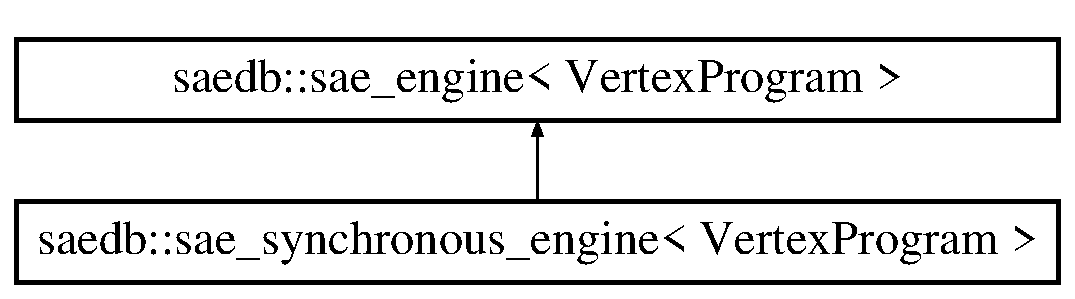
\includegraphics[height=2.000000cm]{d7/d39/classsaedb_1_1sae__synchronous__engine}
\end{center}
\end{figure}
\subsection*{Public Types}
\begin{DoxyCompactItemize}
\item 
typedef Vertex\-Program \hyperlink{classsaedb_1_1sae__synchronous__engine_a9acef979358002e4497dfc877b9fca81}{vertex\-\_\-program\-\_\-type}
\item 
typedef Vertex\-Program\-::gather\-\_\-type \hyperlink{classsaedb_1_1sae__synchronous__engine_a93815ca5d2b8fb54e1dbeda9595e852f}{gather\-\_\-type}
\item 
typedef Vertex\-Program\-::message\-\_\-type \hyperlink{classsaedb_1_1sae__synchronous__engine_ac357ebb2c5a1d064c39189cf66ea3115}{message\-\_\-type}
\item 
typedef \\*
Vertex\-Program\-::vertex\-\_\-data\-\_\-type \hyperlink{classsaedb_1_1sae__synchronous__engine_a2656a04cb1413ab13189a4ea47accdb6}{vertex\-\_\-data\-\_\-type}
\item 
typedef \\*
Vertex\-Program\-::edge\-\_\-data\-\_\-type \hyperlink{classsaedb_1_1sae__synchronous__engine_a1dc041ad51a5c58fc1a2b58b962069f7}{edge\-\_\-data\-\_\-type}
\item 
typedef Vertex\-Program\-::graph\-\_\-type \hyperlink{classsaedb_1_1sae__synchronous__engine_a1eb5ce9b2d9118a21a615211fb026a0e}{graph\-\_\-type}
\item 
typedef \hyperlink{structsaedb_1_1sae__graph_1_1vertex__type}{graph\-\_\-type\-::vertex\-\_\-type} \hyperlink{classsaedb_1_1sae__synchronous__engine_af1ef5f965b2a0f31a1dec2d6125a0b1d}{vertex\-\_\-type}
\item 
typedef \hyperlink{classsaedb_1_1sae__graph_1_1edge__type}{graph\-\_\-type\-::edge\-\_\-type} \hyperlink{classsaedb_1_1sae__synchronous__engine_afc24e00d4e98d9bc1b8b6634d94f13e8}{edge\-\_\-type}
\item 
typedef \hyperlink{classsaedb_1_1sae__graph_afcd2ad6444e374e40a7a5ee4c46be052}{graph\-\_\-type\-::lvid\-\_\-type} \hyperlink{classsaedb_1_1sae__synchronous__engine_a620457f95f0672c538683e94bf97fa2b}{lvid\-\_\-type}
\item 
typedef \hyperlink{classsaedb_1_1context}{context}\\*
$<$ \hyperlink{classsaedb_1_1sae__synchronous__engine}{sae\-\_\-synchronous\-\_\-engine} $>$ \hyperlink{classsaedb_1_1sae__synchronous__engine_a82839f59e66261a2b6f9ae981036e674}{context\-\_\-type}
\end{DoxyCompactItemize}
\subsection*{Public Member Functions}
\begin{DoxyCompactItemize}
\item 
\hyperlink{classsaedb_1_1sae__synchronous__engine_a5f0b83dfbba3033caf57ad3cbfe7de14}{sae\-\_\-synchronous\-\_\-engine} (\hyperlink{classsaedb_1_1sae__synchronous__engine_a1eb5ce9b2d9118a21a615211fb026a0e}{graph\-\_\-type} \&graph)
\item 
void \hyperlink{classsaedb_1_1sae__synchronous__engine_ae6ad2329d41adb55a040ea4a5b667fac}{start} ()
\end{DoxyCompactItemize}
\subsection*{Friends}
\begin{DoxyCompactItemize}
\item 
class \hyperlink{classsaedb_1_1sae__synchronous__engine_a72bdaebdaeffea541642d5d80c4ab985}{context$<$ sae\-\_\-synchronous\-\_\-engine $>$}
\end{DoxyCompactItemize}


\subsection{Detailed Description}
\subsubsection*{template$<$typename Vertex\-Program$>$class saedb\-::sae\-\_\-synchronous\-\_\-engine$<$ Vertex\-Program $>$}



Definition at line 11 of file synchronous\-\_\-engine.\-cpp.



\subsection{Member Typedef Documentation}
\hypertarget{classsaedb_1_1sae__synchronous__engine_a82839f59e66261a2b6f9ae981036e674}{\index{saedb\-::sae\-\_\-synchronous\-\_\-engine@{saedb\-::sae\-\_\-synchronous\-\_\-engine}!context\-\_\-type@{context\-\_\-type}}
\index{context\-\_\-type@{context\-\_\-type}!saedb::sae_synchronous_engine@{saedb\-::sae\-\_\-synchronous\-\_\-engine}}
\subsubsection[{context\-\_\-type}]{\setlength{\rightskip}{0pt plus 5cm}template$<$typename Vertex\-Program$>$ typedef {\bf context}$<${\bf sae\-\_\-synchronous\-\_\-engine}$>$ {\bf saedb\-::sae\-\_\-synchronous\-\_\-engine}$<$ Vertex\-Program $>$\-::{\bf context\-\_\-type}}}\label{d7/d39/classsaedb_1_1sae__synchronous__engine_a82839f59e66261a2b6f9ae981036e674}


Definition at line 25 of file synchronous\-\_\-engine.\-cpp.

\hypertarget{classsaedb_1_1sae__synchronous__engine_a1dc041ad51a5c58fc1a2b58b962069f7}{\index{saedb\-::sae\-\_\-synchronous\-\_\-engine@{saedb\-::sae\-\_\-synchronous\-\_\-engine}!edge\-\_\-data\-\_\-type@{edge\-\_\-data\-\_\-type}}
\index{edge\-\_\-data\-\_\-type@{edge\-\_\-data\-\_\-type}!saedb::sae_synchronous_engine@{saedb\-::sae\-\_\-synchronous\-\_\-engine}}
\subsubsection[{edge\-\_\-data\-\_\-type}]{\setlength{\rightskip}{0pt plus 5cm}template$<$typename Vertex\-Program$>$ typedef Vertex\-Program\-::edge\-\_\-data\-\_\-type {\bf saedb\-::sae\-\_\-synchronous\-\_\-engine}$<$ Vertex\-Program $>$\-::{\bf edge\-\_\-data\-\_\-type}}}\label{d7/d39/classsaedb_1_1sae__synchronous__engine_a1dc041ad51a5c58fc1a2b58b962069f7}


Definition at line 19 of file synchronous\-\_\-engine.\-cpp.

\hypertarget{classsaedb_1_1sae__synchronous__engine_afc24e00d4e98d9bc1b8b6634d94f13e8}{\index{saedb\-::sae\-\_\-synchronous\-\_\-engine@{saedb\-::sae\-\_\-synchronous\-\_\-engine}!edge\-\_\-type@{edge\-\_\-type}}
\index{edge\-\_\-type@{edge\-\_\-type}!saedb::sae_synchronous_engine@{saedb\-::sae\-\_\-synchronous\-\_\-engine}}
\subsubsection[{edge\-\_\-type}]{\setlength{\rightskip}{0pt plus 5cm}template$<$typename Vertex\-Program$>$ typedef {\bf graph\-\_\-type\-::edge\-\_\-type} {\bf saedb\-::sae\-\_\-synchronous\-\_\-engine}$<$ Vertex\-Program $>$\-::{\bf edge\-\_\-type}}}\label{d7/d39/classsaedb_1_1sae__synchronous__engine_afc24e00d4e98d9bc1b8b6634d94f13e8}


Definition at line 22 of file synchronous\-\_\-engine.\-cpp.

\hypertarget{classsaedb_1_1sae__synchronous__engine_a93815ca5d2b8fb54e1dbeda9595e852f}{\index{saedb\-::sae\-\_\-synchronous\-\_\-engine@{saedb\-::sae\-\_\-synchronous\-\_\-engine}!gather\-\_\-type@{gather\-\_\-type}}
\index{gather\-\_\-type@{gather\-\_\-type}!saedb::sae_synchronous_engine@{saedb\-::sae\-\_\-synchronous\-\_\-engine}}
\subsubsection[{gather\-\_\-type}]{\setlength{\rightskip}{0pt plus 5cm}template$<$typename Vertex\-Program$>$ typedef Vertex\-Program\-::gather\-\_\-type {\bf saedb\-::sae\-\_\-synchronous\-\_\-engine}$<$ Vertex\-Program $>$\-::{\bf gather\-\_\-type}}}\label{d7/d39/classsaedb_1_1sae__synchronous__engine_a93815ca5d2b8fb54e1dbeda9595e852f}


Definition at line 16 of file synchronous\-\_\-engine.\-cpp.

\hypertarget{classsaedb_1_1sae__synchronous__engine_a1eb5ce9b2d9118a21a615211fb026a0e}{\index{saedb\-::sae\-\_\-synchronous\-\_\-engine@{saedb\-::sae\-\_\-synchronous\-\_\-engine}!graph\-\_\-type@{graph\-\_\-type}}
\index{graph\-\_\-type@{graph\-\_\-type}!saedb::sae_synchronous_engine@{saedb\-::sae\-\_\-synchronous\-\_\-engine}}
\subsubsection[{graph\-\_\-type}]{\setlength{\rightskip}{0pt plus 5cm}template$<$typename Vertex\-Program$>$ typedef Vertex\-Program\-::graph\-\_\-type {\bf saedb\-::sae\-\_\-synchronous\-\_\-engine}$<$ Vertex\-Program $>$\-::{\bf graph\-\_\-type}}}\label{d7/d39/classsaedb_1_1sae__synchronous__engine_a1eb5ce9b2d9118a21a615211fb026a0e}


Definition at line 20 of file synchronous\-\_\-engine.\-cpp.

\hypertarget{classsaedb_1_1sae__synchronous__engine_a620457f95f0672c538683e94bf97fa2b}{\index{saedb\-::sae\-\_\-synchronous\-\_\-engine@{saedb\-::sae\-\_\-synchronous\-\_\-engine}!lvid\-\_\-type@{lvid\-\_\-type}}
\index{lvid\-\_\-type@{lvid\-\_\-type}!saedb::sae_synchronous_engine@{saedb\-::sae\-\_\-synchronous\-\_\-engine}}
\subsubsection[{lvid\-\_\-type}]{\setlength{\rightskip}{0pt plus 5cm}template$<$typename Vertex\-Program$>$ typedef {\bf graph\-\_\-type\-::lvid\-\_\-type} {\bf saedb\-::sae\-\_\-synchronous\-\_\-engine}$<$ Vertex\-Program $>$\-::{\bf lvid\-\_\-type}}}\label{d7/d39/classsaedb_1_1sae__synchronous__engine_a620457f95f0672c538683e94bf97fa2b}


Definition at line 24 of file synchronous\-\_\-engine.\-cpp.

\hypertarget{classsaedb_1_1sae__synchronous__engine_ac357ebb2c5a1d064c39189cf66ea3115}{\index{saedb\-::sae\-\_\-synchronous\-\_\-engine@{saedb\-::sae\-\_\-synchronous\-\_\-engine}!message\-\_\-type@{message\-\_\-type}}
\index{message\-\_\-type@{message\-\_\-type}!saedb::sae_synchronous_engine@{saedb\-::sae\-\_\-synchronous\-\_\-engine}}
\subsubsection[{message\-\_\-type}]{\setlength{\rightskip}{0pt plus 5cm}template$<$typename Vertex\-Program$>$ typedef Vertex\-Program\-::message\-\_\-type {\bf saedb\-::sae\-\_\-synchronous\-\_\-engine}$<$ Vertex\-Program $>$\-::{\bf message\-\_\-type}}}\label{d7/d39/classsaedb_1_1sae__synchronous__engine_ac357ebb2c5a1d064c39189cf66ea3115}


Definition at line 17 of file synchronous\-\_\-engine.\-cpp.

\hypertarget{classsaedb_1_1sae__synchronous__engine_a2656a04cb1413ab13189a4ea47accdb6}{\index{saedb\-::sae\-\_\-synchronous\-\_\-engine@{saedb\-::sae\-\_\-synchronous\-\_\-engine}!vertex\-\_\-data\-\_\-type@{vertex\-\_\-data\-\_\-type}}
\index{vertex\-\_\-data\-\_\-type@{vertex\-\_\-data\-\_\-type}!saedb::sae_synchronous_engine@{saedb\-::sae\-\_\-synchronous\-\_\-engine}}
\subsubsection[{vertex\-\_\-data\-\_\-type}]{\setlength{\rightskip}{0pt plus 5cm}template$<$typename Vertex\-Program$>$ typedef Vertex\-Program\-::vertex\-\_\-data\-\_\-type {\bf saedb\-::sae\-\_\-synchronous\-\_\-engine}$<$ Vertex\-Program $>$\-::{\bf vertex\-\_\-data\-\_\-type}}}\label{d7/d39/classsaedb_1_1sae__synchronous__engine_a2656a04cb1413ab13189a4ea47accdb6}


Definition at line 18 of file synchronous\-\_\-engine.\-cpp.

\hypertarget{classsaedb_1_1sae__synchronous__engine_a9acef979358002e4497dfc877b9fca81}{\index{saedb\-::sae\-\_\-synchronous\-\_\-engine@{saedb\-::sae\-\_\-synchronous\-\_\-engine}!vertex\-\_\-program\-\_\-type@{vertex\-\_\-program\-\_\-type}}
\index{vertex\-\_\-program\-\_\-type@{vertex\-\_\-program\-\_\-type}!saedb::sae_synchronous_engine@{saedb\-::sae\-\_\-synchronous\-\_\-engine}}
\subsubsection[{vertex\-\_\-program\-\_\-type}]{\setlength{\rightskip}{0pt plus 5cm}template$<$typename Vertex\-Program$>$ typedef Vertex\-Program {\bf saedb\-::sae\-\_\-synchronous\-\_\-engine}$<$ Vertex\-Program $>$\-::{\bf vertex\-\_\-program\-\_\-type}}}\label{d7/d39/classsaedb_1_1sae__synchronous__engine_a9acef979358002e4497dfc877b9fca81}


Definition at line 15 of file synchronous\-\_\-engine.\-cpp.

\hypertarget{classsaedb_1_1sae__synchronous__engine_af1ef5f965b2a0f31a1dec2d6125a0b1d}{\index{saedb\-::sae\-\_\-synchronous\-\_\-engine@{saedb\-::sae\-\_\-synchronous\-\_\-engine}!vertex\-\_\-type@{vertex\-\_\-type}}
\index{vertex\-\_\-type@{vertex\-\_\-type}!saedb::sae_synchronous_engine@{saedb\-::sae\-\_\-synchronous\-\_\-engine}}
\subsubsection[{vertex\-\_\-type}]{\setlength{\rightskip}{0pt plus 5cm}template$<$typename Vertex\-Program$>$ typedef {\bf graph\-\_\-type\-::vertex\-\_\-type} {\bf saedb\-::sae\-\_\-synchronous\-\_\-engine}$<$ Vertex\-Program $>$\-::{\bf vertex\-\_\-type}}}\label{d7/d39/classsaedb_1_1sae__synchronous__engine_af1ef5f965b2a0f31a1dec2d6125a0b1d}


Definition at line 21 of file synchronous\-\_\-engine.\-cpp.



\subsection{Constructor \& Destructor Documentation}
\hypertarget{classsaedb_1_1sae__synchronous__engine_a5f0b83dfbba3033caf57ad3cbfe7de14}{\index{saedb\-::sae\-\_\-synchronous\-\_\-engine@{saedb\-::sae\-\_\-synchronous\-\_\-engine}!sae\-\_\-synchronous\-\_\-engine@{sae\-\_\-synchronous\-\_\-engine}}
\index{sae\-\_\-synchronous\-\_\-engine@{sae\-\_\-synchronous\-\_\-engine}!saedb::sae_synchronous_engine@{saedb\-::sae\-\_\-synchronous\-\_\-engine}}
\subsubsection[{sae\-\_\-synchronous\-\_\-engine}]{\setlength{\rightskip}{0pt plus 5cm}template$<$typename Vertex\-Program $>$ {\bf saedb\-::sae\-\_\-synchronous\-\_\-engine}$<$ Vertex\-Program $>$\-::{\bf sae\-\_\-synchronous\-\_\-engine} (
\begin{DoxyParamCaption}
\item[{{\bf graph\-\_\-type} \&}]{graph}
\end{DoxyParamCaption}
)}}\label{d7/d39/classsaedb_1_1sae__synchronous__engine_a5f0b83dfbba3033caf57ad3cbfe7de14}


Definition at line 57 of file synchronous\-\_\-engine.\-cpp.



\subsection{Member Function Documentation}
\hypertarget{classsaedb_1_1sae__synchronous__engine_ae6ad2329d41adb55a040ea4a5b667fac}{\index{saedb\-::sae\-\_\-synchronous\-\_\-engine@{saedb\-::sae\-\_\-synchronous\-\_\-engine}!start@{start}}
\index{start@{start}!saedb::sae_synchronous_engine@{saedb\-::sae\-\_\-synchronous\-\_\-engine}}
\subsubsection[{start}]{\setlength{\rightskip}{0pt plus 5cm}template$<$typename Vertex\-Program $>$ void {\bf saedb\-::sae\-\_\-synchronous\-\_\-engine}$<$ Vertex\-Program $>$\-::start (
\begin{DoxyParamCaption}
{}
\end{DoxyParamCaption}
)\hspace{0.3cm}{\ttfamily [virtual]}}}\label{d7/d39/classsaedb_1_1sae__synchronous__engine_ae6ad2329d41adb55a040ea4a5b667fac}


Implements \hyperlink{classsaedb_1_1sae__engine_aa4e0b1b7ab5dcdf3baa48ae0d798b30b}{saedb\-::sae\-\_\-engine$<$ Vertex\-Program $>$}.



Definition at line 64 of file synchronous\-\_\-engine.\-cpp.



\subsection{Friends And Related Function Documentation}
\hypertarget{classsaedb_1_1sae__synchronous__engine_a72bdaebdaeffea541642d5d80c4ab985}{\index{saedb\-::sae\-\_\-synchronous\-\_\-engine@{saedb\-::sae\-\_\-synchronous\-\_\-engine}!context$<$ sae\-\_\-synchronous\-\_\-engine $>$@{context$<$ sae\-\_\-synchronous\-\_\-engine $>$}}
\index{context$<$ sae\-\_\-synchronous\-\_\-engine $>$@{context$<$ sae\-\_\-synchronous\-\_\-engine $>$}!saedb::sae_synchronous_engine@{saedb\-::sae\-\_\-synchronous\-\_\-engine}}
\subsubsection[{context$<$ sae\-\_\-synchronous\-\_\-engine $>$}]{\setlength{\rightskip}{0pt plus 5cm}template$<$typename Vertex\-Program$>$ friend class {\bf context}$<$ {\bf sae\-\_\-synchronous\-\_\-engine} $>$\hspace{0.3cm}{\ttfamily [friend]}}}\label{d7/d39/classsaedb_1_1sae__synchronous__engine_a72bdaebdaeffea541642d5d80c4ab985}


Definition at line 26 of file synchronous\-\_\-engine.\-cpp.



The documentation for this class was generated from the following file\-:\begin{DoxyCompactItemize}
\item 
src/saedb/\hyperlink{synchronous__engine_8cpp}{synchronous\-\_\-engine.\-cpp}\end{DoxyCompactItemize}

\hypertarget{structsaedb_1_1sae__graph_1_1vertex__type}{\section{saedb\-:\-:sae\-\_\-graph$<$ Vertex\-Data, Edge\-Data $>$\-:\-:vertex\-\_\-type Struct Reference}
\label{d1/d90/structsaedb_1_1sae__graph_1_1vertex__type}\index{saedb\-::sae\-\_\-graph$<$ Vertex\-Data, Edge\-Data $>$\-::vertex\-\_\-type@{saedb\-::sae\-\_\-graph$<$ Vertex\-Data, Edge\-Data $>$\-::vertex\-\_\-type}}
}


{\ttfamily \#include $<$graph.\-hpp$>$}

\subsection*{Public Member Functions}
\begin{DoxyCompactItemize}
\item 
\hyperlink{structsaedb_1_1sae__graph_1_1vertex__type_ab6014b10ce17d692e923dec61d0da1cc}{vertex\-\_\-type} (\hyperlink{classsaedb_1_1sae__graph}{sae\-\_\-graph} \&\hyperlink{structsaedb_1_1sae__graph_1_1vertex__type_a5977862a541ff4fe90999fbf49d287dd}{graph\-\_\-ref}, \hyperlink{classsaedb_1_1sae__graph_afcd2ad6444e374e40a7a5ee4c46be052}{lvid\-\_\-type} \hyperlink{structsaedb_1_1sae__graph_1_1vertex__type_a580dbdb1a1037a94f7ee66d942d679cc}{lvid})
\item 
\hyperlink{structsaedb_1_1sae__graph_1_1vertex__type_a94f186a7bf16ef32e86d15b3eca4c220}{vertex\-\_\-type} ()
\item 
bool \hyperlink{structsaedb_1_1sae__graph_1_1vertex__type_acb6817d125e4c5e7dadf0df0beb1ba92}{operator==} (\hyperlink{structsaedb_1_1sae__graph_1_1vertex__type}{vertex\-\_\-type} \&v) const 
\item 
const \hyperlink{classsaedb_1_1sae__graph_a8e9dfeb979f49c35d427f364fb3f69f5}{vertex\-\_\-data\-\_\-type} \& \hyperlink{structsaedb_1_1sae__graph_1_1vertex__type_a794a1ed375ecbe057d1bb6b9e63eb9d8}{data} () const 
\item 
\hyperlink{classsaedb_1_1sae__graph_a8e9dfeb979f49c35d427f364fb3f69f5}{vertex\-\_\-data\-\_\-type} \& \hyperlink{structsaedb_1_1sae__graph_1_1vertex__type_a23a4c9c51691ba351ef0d5ad573051a6}{data} ()
\item 
size\-\_\-t \hyperlink{structsaedb_1_1sae__graph_1_1vertex__type_af64b2e0509849b27df833fe2c4bbfd93}{num\-\_\-in\-\_\-edges} () const 
\item 
size\-\_\-t \hyperlink{structsaedb_1_1sae__graph_1_1vertex__type_aea5f50d441f1b97d83e4bcd0137760d2}{num\-\_\-out\-\_\-edges} () const 
\item 
\hyperlink{classsaedb_1_1sae__graph_a2f9a7bf2db556689f1cd9de9562ff41f}{vertex\-\_\-id\-\_\-type} \hyperlink{structsaedb_1_1sae__graph_1_1vertex__type_ae6b591fd40d4f080ee1c07741327ba67}{id} () const 
\item 
vector$<$ \hyperlink{classsaedb_1_1sae__graph_1_1edge__type}{edge\-\_\-type} $>$ \hyperlink{structsaedb_1_1sae__graph_1_1vertex__type_a0a70b2799c2309519c79eb805476c1aa}{in\-\_\-edges} ()
\item 
vector$<$ \hyperlink{classsaedb_1_1sae__graph_1_1edge__type}{edge\-\_\-type} $>$ \hyperlink{structsaedb_1_1sae__graph_1_1vertex__type_aa81f6d3ddc7905990c767628e1eb838d}{out\-\_\-edges} ()
\item 
\hyperlink{classsaedb_1_1sae__graph_afcd2ad6444e374e40a7a5ee4c46be052}{lvid\-\_\-type} \hyperlink{structsaedb_1_1sae__graph_1_1vertex__type_ac295ff8f407594f3f1013acd41fbf48c}{local\-\_\-id} () const 
\end{DoxyCompactItemize}
\subsection*{Public Attributes}
\begin{DoxyCompactItemize}
\item 
\hyperlink{classsaedb_1_1sae__graph}{sae\-\_\-graph} \& \hyperlink{structsaedb_1_1sae__graph_1_1vertex__type_a5977862a541ff4fe90999fbf49d287dd}{graph\-\_\-ref}
\item 
\hyperlink{classsaedb_1_1sae__graph_afcd2ad6444e374e40a7a5ee4c46be052}{lvid\-\_\-type} \hyperlink{structsaedb_1_1sae__graph_1_1vertex__type_a580dbdb1a1037a94f7ee66d942d679cc}{lvid}
\end{DoxyCompactItemize}


\subsection{Detailed Description}
\subsubsection*{template$<$typename Vertex\-Data, typename Edge\-Data$>$struct saedb\-::sae\-\_\-graph$<$ Vertex\-Data, Edge\-Data $>$\-::vertex\-\_\-type}



Definition at line 116 of file graph.\-hpp.



\subsection{Constructor \& Destructor Documentation}
\hypertarget{structsaedb_1_1sae__graph_1_1vertex__type_ab6014b10ce17d692e923dec61d0da1cc}{\index{saedb\-::sae\-\_\-graph\-::vertex\-\_\-type@{saedb\-::sae\-\_\-graph\-::vertex\-\_\-type}!vertex\-\_\-type@{vertex\-\_\-type}}
\index{vertex\-\_\-type@{vertex\-\_\-type}!saedb::sae_graph::vertex_type@{saedb\-::sae\-\_\-graph\-::vertex\-\_\-type}}
\subsubsection[{vertex\-\_\-type}]{\setlength{\rightskip}{0pt plus 5cm}template$<$typename Vertex\-Data , typename Edge\-Data $>$ {\bf saedb\-::sae\-\_\-graph}$<$ Vertex\-Data, Edge\-Data $>$\-::vertex\-\_\-type\-::vertex\-\_\-type (
\begin{DoxyParamCaption}
\item[{{\bf sae\-\_\-graph} \&}]{graph\-\_\-ref, }
\item[{{\bf lvid\-\_\-type}}]{lvid}
\end{DoxyParamCaption}
)\hspace{0.3cm}{\ttfamily [inline]}}}\label{d1/d90/structsaedb_1_1sae__graph_1_1vertex__type_ab6014b10ce17d692e923dec61d0da1cc}


Definition at line 120 of file graph.\-hpp.

\hypertarget{structsaedb_1_1sae__graph_1_1vertex__type_a94f186a7bf16ef32e86d15b3eca4c220}{\index{saedb\-::sae\-\_\-graph\-::vertex\-\_\-type@{saedb\-::sae\-\_\-graph\-::vertex\-\_\-type}!vertex\-\_\-type@{vertex\-\_\-type}}
\index{vertex\-\_\-type@{vertex\-\_\-type}!saedb::sae_graph::vertex_type@{saedb\-::sae\-\_\-graph\-::vertex\-\_\-type}}
\subsubsection[{vertex\-\_\-type}]{\setlength{\rightskip}{0pt plus 5cm}template$<$typename Vertex\-Data , typename Edge\-Data $>$ {\bf saedb\-::sae\-\_\-graph}$<$ Vertex\-Data, Edge\-Data $>$\-::vertex\-\_\-type\-::vertex\-\_\-type (
\begin{DoxyParamCaption}
{}
\end{DoxyParamCaption}
)\hspace{0.3cm}{\ttfamily [inline]}}}\label{d1/d90/structsaedb_1_1sae__graph_1_1vertex__type_a94f186a7bf16ef32e86d15b3eca4c220}


Definition at line 123 of file graph.\-hpp.



\subsection{Member Function Documentation}
\hypertarget{structsaedb_1_1sae__graph_1_1vertex__type_a794a1ed375ecbe057d1bb6b9e63eb9d8}{\index{saedb\-::sae\-\_\-graph\-::vertex\-\_\-type@{saedb\-::sae\-\_\-graph\-::vertex\-\_\-type}!data@{data}}
\index{data@{data}!saedb::sae_graph::vertex_type@{saedb\-::sae\-\_\-graph\-::vertex\-\_\-type}}
\subsubsection[{data}]{\setlength{\rightskip}{0pt plus 5cm}template$<$typename Vertex\-Data , typename Edge\-Data $>$ const {\bf vertex\-\_\-data\-\_\-type}\& {\bf saedb\-::sae\-\_\-graph}$<$ Vertex\-Data, Edge\-Data $>$\-::vertex\-\_\-type\-::data (
\begin{DoxyParamCaption}
{}
\end{DoxyParamCaption}
) const\hspace{0.3cm}{\ttfamily [inline]}}}\label{d1/d90/structsaedb_1_1sae__graph_1_1vertex__type_a794a1ed375ecbe057d1bb6b9e63eb9d8}


Definition at line 129 of file graph.\-hpp.

\hypertarget{structsaedb_1_1sae__graph_1_1vertex__type_a23a4c9c51691ba351ef0d5ad573051a6}{\index{saedb\-::sae\-\_\-graph\-::vertex\-\_\-type@{saedb\-::sae\-\_\-graph\-::vertex\-\_\-type}!data@{data}}
\index{data@{data}!saedb::sae_graph::vertex_type@{saedb\-::sae\-\_\-graph\-::vertex\-\_\-type}}
\subsubsection[{data}]{\setlength{\rightskip}{0pt plus 5cm}template$<$typename Vertex\-Data , typename Edge\-Data $>$ {\bf vertex\-\_\-data\-\_\-type}\& {\bf saedb\-::sae\-\_\-graph}$<$ Vertex\-Data, Edge\-Data $>$\-::vertex\-\_\-type\-::data (
\begin{DoxyParamCaption}
{}
\end{DoxyParamCaption}
)\hspace{0.3cm}{\ttfamily [inline]}}}\label{d1/d90/structsaedb_1_1sae__graph_1_1vertex__type_a23a4c9c51691ba351ef0d5ad573051a6}


Definition at line 133 of file graph.\-hpp.

\hypertarget{structsaedb_1_1sae__graph_1_1vertex__type_ae6b591fd40d4f080ee1c07741327ba67}{\index{saedb\-::sae\-\_\-graph\-::vertex\-\_\-type@{saedb\-::sae\-\_\-graph\-::vertex\-\_\-type}!id@{id}}
\index{id@{id}!saedb::sae_graph::vertex_type@{saedb\-::sae\-\_\-graph\-::vertex\-\_\-type}}
\subsubsection[{id}]{\setlength{\rightskip}{0pt plus 5cm}template$<$typename Vertex\-Data , typename Edge\-Data $>$ {\bf vertex\-\_\-id\-\_\-type} {\bf saedb\-::sae\-\_\-graph}$<$ Vertex\-Data, Edge\-Data $>$\-::vertex\-\_\-type\-::id (
\begin{DoxyParamCaption}
{}
\end{DoxyParamCaption}
) const\hspace{0.3cm}{\ttfamily [inline]}}}\label{d1/d90/structsaedb_1_1sae__graph_1_1vertex__type_ae6b591fd40d4f080ee1c07741327ba67}


Definition at line 143 of file graph.\-hpp.

\hypertarget{structsaedb_1_1sae__graph_1_1vertex__type_a0a70b2799c2309519c79eb805476c1aa}{\index{saedb\-::sae\-\_\-graph\-::vertex\-\_\-type@{saedb\-::sae\-\_\-graph\-::vertex\-\_\-type}!in\-\_\-edges@{in\-\_\-edges}}
\index{in\-\_\-edges@{in\-\_\-edges}!saedb::sae_graph::vertex_type@{saedb\-::sae\-\_\-graph\-::vertex\-\_\-type}}
\subsubsection[{in\-\_\-edges}]{\setlength{\rightskip}{0pt plus 5cm}template$<$typename Vertex\-Data , typename Edge\-Data $>$ vector$<${\bf edge\-\_\-type}$>$ {\bf saedb\-::sae\-\_\-graph}$<$ Vertex\-Data, Edge\-Data $>$\-::vertex\-\_\-type\-::in\-\_\-edges (
\begin{DoxyParamCaption}
{}
\end{DoxyParamCaption}
)\hspace{0.3cm}{\ttfamily [inline]}}}\label{d1/d90/structsaedb_1_1sae__graph_1_1vertex__type_a0a70b2799c2309519c79eb805476c1aa}


Definition at line 147 of file graph.\-hpp.

\hypertarget{structsaedb_1_1sae__graph_1_1vertex__type_ac295ff8f407594f3f1013acd41fbf48c}{\index{saedb\-::sae\-\_\-graph\-::vertex\-\_\-type@{saedb\-::sae\-\_\-graph\-::vertex\-\_\-type}!local\-\_\-id@{local\-\_\-id}}
\index{local\-\_\-id@{local\-\_\-id}!saedb::sae_graph::vertex_type@{saedb\-::sae\-\_\-graph\-::vertex\-\_\-type}}
\subsubsection[{local\-\_\-id}]{\setlength{\rightskip}{0pt plus 5cm}template$<$typename Vertex\-Data , typename Edge\-Data $>$ {\bf lvid\-\_\-type} {\bf saedb\-::sae\-\_\-graph}$<$ Vertex\-Data, Edge\-Data $>$\-::vertex\-\_\-type\-::local\-\_\-id (
\begin{DoxyParamCaption}
{}
\end{DoxyParamCaption}
) const\hspace{0.3cm}{\ttfamily [inline]}}}\label{d1/d90/structsaedb_1_1sae__graph_1_1vertex__type_ac295ff8f407594f3f1013acd41fbf48c}


Definition at line 155 of file graph.\-hpp.

\hypertarget{structsaedb_1_1sae__graph_1_1vertex__type_af64b2e0509849b27df833fe2c4bbfd93}{\index{saedb\-::sae\-\_\-graph\-::vertex\-\_\-type@{saedb\-::sae\-\_\-graph\-::vertex\-\_\-type}!num\-\_\-in\-\_\-edges@{num\-\_\-in\-\_\-edges}}
\index{num\-\_\-in\-\_\-edges@{num\-\_\-in\-\_\-edges}!saedb::sae_graph::vertex_type@{saedb\-::sae\-\_\-graph\-::vertex\-\_\-type}}
\subsubsection[{num\-\_\-in\-\_\-edges}]{\setlength{\rightskip}{0pt plus 5cm}template$<$typename Vertex\-Data , typename Edge\-Data $>$ size\-\_\-t {\bf saedb\-::sae\-\_\-graph}$<$ Vertex\-Data, Edge\-Data $>$\-::vertex\-\_\-type\-::num\-\_\-in\-\_\-edges (
\begin{DoxyParamCaption}
{}
\end{DoxyParamCaption}
) const\hspace{0.3cm}{\ttfamily [inline]}}}\label{d1/d90/structsaedb_1_1sae__graph_1_1vertex__type_af64b2e0509849b27df833fe2c4bbfd93}


Definition at line 137 of file graph.\-hpp.

\hypertarget{structsaedb_1_1sae__graph_1_1vertex__type_aea5f50d441f1b97d83e4bcd0137760d2}{\index{saedb\-::sae\-\_\-graph\-::vertex\-\_\-type@{saedb\-::sae\-\_\-graph\-::vertex\-\_\-type}!num\-\_\-out\-\_\-edges@{num\-\_\-out\-\_\-edges}}
\index{num\-\_\-out\-\_\-edges@{num\-\_\-out\-\_\-edges}!saedb::sae_graph::vertex_type@{saedb\-::sae\-\_\-graph\-::vertex\-\_\-type}}
\subsubsection[{num\-\_\-out\-\_\-edges}]{\setlength{\rightskip}{0pt plus 5cm}template$<$typename Vertex\-Data , typename Edge\-Data $>$ size\-\_\-t {\bf saedb\-::sae\-\_\-graph}$<$ Vertex\-Data, Edge\-Data $>$\-::vertex\-\_\-type\-::num\-\_\-out\-\_\-edges (
\begin{DoxyParamCaption}
{}
\end{DoxyParamCaption}
) const\hspace{0.3cm}{\ttfamily [inline]}}}\label{d1/d90/structsaedb_1_1sae__graph_1_1vertex__type_aea5f50d441f1b97d83e4bcd0137760d2}


Definition at line 140 of file graph.\-hpp.

\hypertarget{structsaedb_1_1sae__graph_1_1vertex__type_acb6817d125e4c5e7dadf0df0beb1ba92}{\index{saedb\-::sae\-\_\-graph\-::vertex\-\_\-type@{saedb\-::sae\-\_\-graph\-::vertex\-\_\-type}!operator==@{operator==}}
\index{operator==@{operator==}!saedb::sae_graph::vertex_type@{saedb\-::sae\-\_\-graph\-::vertex\-\_\-type}}
\subsubsection[{operator==}]{\setlength{\rightskip}{0pt plus 5cm}template$<$typename Vertex\-Data , typename Edge\-Data $>$ bool {\bf saedb\-::sae\-\_\-graph}$<$ Vertex\-Data, Edge\-Data $>$\-::vertex\-\_\-type\-::operator== (
\begin{DoxyParamCaption}
\item[{{\bf vertex\-\_\-type} \&}]{v}
\end{DoxyParamCaption}
) const\hspace{0.3cm}{\ttfamily [inline]}}}\label{d1/d90/structsaedb_1_1sae__graph_1_1vertex__type_acb6817d125e4c5e7dadf0df0beb1ba92}


Definition at line 125 of file graph.\-hpp.

\hypertarget{structsaedb_1_1sae__graph_1_1vertex__type_aa81f6d3ddc7905990c767628e1eb838d}{\index{saedb\-::sae\-\_\-graph\-::vertex\-\_\-type@{saedb\-::sae\-\_\-graph\-::vertex\-\_\-type}!out\-\_\-edges@{out\-\_\-edges}}
\index{out\-\_\-edges@{out\-\_\-edges}!saedb::sae_graph::vertex_type@{saedb\-::sae\-\_\-graph\-::vertex\-\_\-type}}
\subsubsection[{out\-\_\-edges}]{\setlength{\rightskip}{0pt plus 5cm}template$<$typename Vertex\-Data , typename Edge\-Data $>$ vector$<${\bf edge\-\_\-type}$>$ {\bf saedb\-::sae\-\_\-graph}$<$ Vertex\-Data, Edge\-Data $>$\-::vertex\-\_\-type\-::out\-\_\-edges (
\begin{DoxyParamCaption}
{}
\end{DoxyParamCaption}
)\hspace{0.3cm}{\ttfamily [inline]}}}\label{d1/d90/structsaedb_1_1sae__graph_1_1vertex__type_aa81f6d3ddc7905990c767628e1eb838d}


Definition at line 151 of file graph.\-hpp.



\subsection{Member Data Documentation}
\hypertarget{structsaedb_1_1sae__graph_1_1vertex__type_a5977862a541ff4fe90999fbf49d287dd}{\index{saedb\-::sae\-\_\-graph\-::vertex\-\_\-type@{saedb\-::sae\-\_\-graph\-::vertex\-\_\-type}!graph\-\_\-ref@{graph\-\_\-ref}}
\index{graph\-\_\-ref@{graph\-\_\-ref}!saedb::sae_graph::vertex_type@{saedb\-::sae\-\_\-graph\-::vertex\-\_\-type}}
\subsubsection[{graph\-\_\-ref}]{\setlength{\rightskip}{0pt plus 5cm}template$<$typename Vertex\-Data , typename Edge\-Data $>$ {\bf sae\-\_\-graph}\& {\bf saedb\-::sae\-\_\-graph}$<$ Vertex\-Data, Edge\-Data $>$\-::vertex\-\_\-type\-::graph\-\_\-ref}}\label{d1/d90/structsaedb_1_1sae__graph_1_1vertex__type_a5977862a541ff4fe90999fbf49d287dd}


Definition at line 117 of file graph.\-hpp.

\hypertarget{structsaedb_1_1sae__graph_1_1vertex__type_a580dbdb1a1037a94f7ee66d942d679cc}{\index{saedb\-::sae\-\_\-graph\-::vertex\-\_\-type@{saedb\-::sae\-\_\-graph\-::vertex\-\_\-type}!lvid@{lvid}}
\index{lvid@{lvid}!saedb::sae_graph::vertex_type@{saedb\-::sae\-\_\-graph\-::vertex\-\_\-type}}
\subsubsection[{lvid}]{\setlength{\rightskip}{0pt plus 5cm}template$<$typename Vertex\-Data , typename Edge\-Data $>$ {\bf lvid\-\_\-type} {\bf saedb\-::sae\-\_\-graph}$<$ Vertex\-Data, Edge\-Data $>$\-::vertex\-\_\-type\-::lvid}}\label{d1/d90/structsaedb_1_1sae__graph_1_1vertex__type_a580dbdb1a1037a94f7ee66d942d679cc}


Definition at line 118 of file graph.\-hpp.



The documentation for this struct was generated from the following file\-:\begin{DoxyCompactItemize}
\item 
src/saedb/\hyperlink{graph_8hpp}{graph.\-hpp}\end{DoxyCompactItemize}

\hypertarget{structsaedb_1_1local__graph_1_1vertex__type}{\section{saedb\-:\-:local\-\_\-graph$<$ Vertex\-Data, Edge\-Data $>$\-:\-:vertex\-\_\-type Struct Reference}
\label{dd/d9a/structsaedb_1_1local__graph_1_1vertex__type}\index{saedb\-::local\-\_\-graph$<$ Vertex\-Data, Edge\-Data $>$\-::vertex\-\_\-type@{saedb\-::local\-\_\-graph$<$ Vertex\-Data, Edge\-Data $>$\-::vertex\-\_\-type}}
}


{\ttfamily \#include $<$local\-\_\-graph.\-hpp$>$}

\subsection*{Public Member Functions}
\begin{DoxyCompactItemize}
\item 
\hyperlink{structsaedb_1_1local__graph_1_1vertex__type_af6dc2c1d477f81b2582a11cf9eec1dde}{vertex\-\_\-type} (\hyperlink{classsaedb_1_1local__graph}{local\-\_\-graph} \&\hyperlink{structsaedb_1_1local__graph_1_1vertex__type_a67948a82fbbd84618e77e73c44775527}{lgraph\-\_\-ref}, \hyperlink{namespacesaedb_ae0f2df508bdfd29505d57534c8ed4a65}{lvid\-\_\-type} \hyperlink{structsaedb_1_1local__graph_1_1vertex__type_adcff5336560c8bc3bafc2a3a0deb0518}{vid})
\item 
const \hyperlink{classsaedb_1_1local__graph_a844bd7c9e27012270a4d6499ff830360}{vertex\-\_\-data\-\_\-type} \& \hyperlink{structsaedb_1_1local__graph_1_1vertex__type_a985dd4c5b7d204921a86c4d77ad9a3fd}{data} () const 
\item 
\hyperlink{classsaedb_1_1local__graph_a844bd7c9e27012270a4d6499ff830360}{vertex\-\_\-data\-\_\-type} \& \hyperlink{structsaedb_1_1local__graph_1_1vertex__type_a4cad1bf0109a5ae5d9228ea6988bba1d}{data} ()
\item 
size\-\_\-t \hyperlink{structsaedb_1_1local__graph_1_1vertex__type_a31ba0b56f07c805b4b315709385160f1}{num\-\_\-in\-\_\-edges} () const 
\item 
size\-\_\-t \hyperlink{structsaedb_1_1local__graph_1_1vertex__type_a8c600b26d48d6a0fd958ce6911ae57e4}{num\-\_\-out\-\_\-edges} () const 
\item 
\hyperlink{namespacesaedb_ae0f2df508bdfd29505d57534c8ed4a65}{lvid\-\_\-type} \hyperlink{structsaedb_1_1local__graph_1_1vertex__type_a3ca972e4f32f004ddf546f5852f22c19}{id} () const 
\item 
edge\-\_\-list\-\_\-type \hyperlink{structsaedb_1_1local__graph_1_1vertex__type_ae5d2a224c06f6a7683f1e5ad6d0e984c}{in\-\_\-edges} ()
\item 
edge\-\_\-list\-\_\-type \hyperlink{structsaedb_1_1local__graph_1_1vertex__type_a0712510cea285500e449e9495e465c30}{out\-\_\-edges} ()
\end{DoxyCompactItemize}
\subsection*{Public Attributes}
\begin{DoxyCompactItemize}
\item 
\hyperlink{classsaedb_1_1local__graph}{local\-\_\-graph} \& \hyperlink{structsaedb_1_1local__graph_1_1vertex__type_a67948a82fbbd84618e77e73c44775527}{lgraph\-\_\-ref}
\item 
\hyperlink{namespacesaedb_ae0f2df508bdfd29505d57534c8ed4a65}{lvid\-\_\-type} \hyperlink{structsaedb_1_1local__graph_1_1vertex__type_adcff5336560c8bc3bafc2a3a0deb0518}{vid}
\end{DoxyCompactItemize}


\subsection{Detailed Description}
\subsubsection*{template$<$typename Vertex\-Data, typename Edge\-Data$>$struct saedb\-::local\-\_\-graph$<$ Vertex\-Data, Edge\-Data $>$\-::vertex\-\_\-type}



Definition at line 54 of file local\-\_\-graph.\-hpp.



\subsection{Constructor \& Destructor Documentation}
\hypertarget{structsaedb_1_1local__graph_1_1vertex__type_af6dc2c1d477f81b2582a11cf9eec1dde}{\index{saedb\-::local\-\_\-graph\-::vertex\-\_\-type@{saedb\-::local\-\_\-graph\-::vertex\-\_\-type}!vertex\-\_\-type@{vertex\-\_\-type}}
\index{vertex\-\_\-type@{vertex\-\_\-type}!saedb::local_graph::vertex_type@{saedb\-::local\-\_\-graph\-::vertex\-\_\-type}}
\subsubsection[{vertex\-\_\-type}]{\setlength{\rightskip}{0pt plus 5cm}template$<$typename Vertex\-Data , typename Edge\-Data $>$ {\bf saedb\-::local\-\_\-graph}$<$ Vertex\-Data, Edge\-Data $>$\-::vertex\-\_\-type\-::vertex\-\_\-type (
\begin{DoxyParamCaption}
\item[{{\bf local\-\_\-graph} \&}]{lgraph\-\_\-ref, }
\item[{{\bf lvid\-\_\-type}}]{vid}
\end{DoxyParamCaption}
)\hspace{0.3cm}{\ttfamily [inline]}}}\label{dd/d9a/structsaedb_1_1local__graph_1_1vertex__type_af6dc2c1d477f81b2582a11cf9eec1dde}


Definition at line 57 of file local\-\_\-graph.\-hpp.



\subsection{Member Function Documentation}
\hypertarget{structsaedb_1_1local__graph_1_1vertex__type_a985dd4c5b7d204921a86c4d77ad9a3fd}{\index{saedb\-::local\-\_\-graph\-::vertex\-\_\-type@{saedb\-::local\-\_\-graph\-::vertex\-\_\-type}!data@{data}}
\index{data@{data}!saedb::local_graph::vertex_type@{saedb\-::local\-\_\-graph\-::vertex\-\_\-type}}
\subsubsection[{data}]{\setlength{\rightskip}{0pt plus 5cm}template$<$typename Vertex\-Data , typename Edge\-Data $>$ const {\bf vertex\-\_\-data\-\_\-type}\& {\bf saedb\-::local\-\_\-graph}$<$ Vertex\-Data, Edge\-Data $>$\-::vertex\-\_\-type\-::data (
\begin{DoxyParamCaption}
{}
\end{DoxyParamCaption}
) const\hspace{0.3cm}{\ttfamily [inline]}}}\label{dd/d9a/structsaedb_1_1local__graph_1_1vertex__type_a985dd4c5b7d204921a86c4d77ad9a3fd}


Definition at line 59 of file local\-\_\-graph.\-hpp.

\hypertarget{structsaedb_1_1local__graph_1_1vertex__type_a4cad1bf0109a5ae5d9228ea6988bba1d}{\index{saedb\-::local\-\_\-graph\-::vertex\-\_\-type@{saedb\-::local\-\_\-graph\-::vertex\-\_\-type}!data@{data}}
\index{data@{data}!saedb::local_graph::vertex_type@{saedb\-::local\-\_\-graph\-::vertex\-\_\-type}}
\subsubsection[{data}]{\setlength{\rightskip}{0pt plus 5cm}template$<$typename Vertex\-Data , typename Edge\-Data $>$ {\bf vertex\-\_\-data\-\_\-type}\& {\bf saedb\-::local\-\_\-graph}$<$ Vertex\-Data, Edge\-Data $>$\-::vertex\-\_\-type\-::data (
\begin{DoxyParamCaption}
{}
\end{DoxyParamCaption}
)\hspace{0.3cm}{\ttfamily [inline]}}}\label{dd/d9a/structsaedb_1_1local__graph_1_1vertex__type_a4cad1bf0109a5ae5d9228ea6988bba1d}


Definition at line 62 of file local\-\_\-graph.\-hpp.

\hypertarget{structsaedb_1_1local__graph_1_1vertex__type_a3ca972e4f32f004ddf546f5852f22c19}{\index{saedb\-::local\-\_\-graph\-::vertex\-\_\-type@{saedb\-::local\-\_\-graph\-::vertex\-\_\-type}!id@{id}}
\index{id@{id}!saedb::local_graph::vertex_type@{saedb\-::local\-\_\-graph\-::vertex\-\_\-type}}
\subsubsection[{id}]{\setlength{\rightskip}{0pt plus 5cm}template$<$typename Vertex\-Data , typename Edge\-Data $>$ {\bf lvid\-\_\-type} {\bf saedb\-::local\-\_\-graph}$<$ Vertex\-Data, Edge\-Data $>$\-::vertex\-\_\-type\-::id (
\begin{DoxyParamCaption}
{}
\end{DoxyParamCaption}
) const\hspace{0.3cm}{\ttfamily [inline]}}}\label{dd/d9a/structsaedb_1_1local__graph_1_1vertex__type_a3ca972e4f32f004ddf546f5852f22c19}


Definition at line 74 of file local\-\_\-graph.\-hpp.

\hypertarget{structsaedb_1_1local__graph_1_1vertex__type_ae5d2a224c06f6a7683f1e5ad6d0e984c}{\index{saedb\-::local\-\_\-graph\-::vertex\-\_\-type@{saedb\-::local\-\_\-graph\-::vertex\-\_\-type}!in\-\_\-edges@{in\-\_\-edges}}
\index{in\-\_\-edges@{in\-\_\-edges}!saedb::local_graph::vertex_type@{saedb\-::local\-\_\-graph\-::vertex\-\_\-type}}
\subsubsection[{in\-\_\-edges}]{\setlength{\rightskip}{0pt plus 5cm}template$<$typename Vertex\-Data , typename Edge\-Data $>$ edge\-\_\-list\-\_\-type {\bf saedb\-::local\-\_\-graph}$<$ Vertex\-Data, Edge\-Data $>$\-::vertex\-\_\-type\-::in\-\_\-edges (
\begin{DoxyParamCaption}
{}
\end{DoxyParamCaption}
)\hspace{0.3cm}{\ttfamily [inline]}}}\label{dd/d9a/structsaedb_1_1local__graph_1_1vertex__type_ae5d2a224c06f6a7683f1e5ad6d0e984c}


Definition at line 78 of file local\-\_\-graph.\-hpp.

\hypertarget{structsaedb_1_1local__graph_1_1vertex__type_a31ba0b56f07c805b4b315709385160f1}{\index{saedb\-::local\-\_\-graph\-::vertex\-\_\-type@{saedb\-::local\-\_\-graph\-::vertex\-\_\-type}!num\-\_\-in\-\_\-edges@{num\-\_\-in\-\_\-edges}}
\index{num\-\_\-in\-\_\-edges@{num\-\_\-in\-\_\-edges}!saedb::local_graph::vertex_type@{saedb\-::local\-\_\-graph\-::vertex\-\_\-type}}
\subsubsection[{num\-\_\-in\-\_\-edges}]{\setlength{\rightskip}{0pt plus 5cm}template$<$typename Vertex\-Data , typename Edge\-Data $>$ size\-\_\-t {\bf saedb\-::local\-\_\-graph}$<$ Vertex\-Data, Edge\-Data $>$\-::vertex\-\_\-type\-::num\-\_\-in\-\_\-edges (
\begin{DoxyParamCaption}
{}
\end{DoxyParamCaption}
) const\hspace{0.3cm}{\ttfamily [inline]}}}\label{dd/d9a/structsaedb_1_1local__graph_1_1vertex__type_a31ba0b56f07c805b4b315709385160f1}


Definition at line 66 of file local\-\_\-graph.\-hpp.

\hypertarget{structsaedb_1_1local__graph_1_1vertex__type_a8c600b26d48d6a0fd958ce6911ae57e4}{\index{saedb\-::local\-\_\-graph\-::vertex\-\_\-type@{saedb\-::local\-\_\-graph\-::vertex\-\_\-type}!num\-\_\-out\-\_\-edges@{num\-\_\-out\-\_\-edges}}
\index{num\-\_\-out\-\_\-edges@{num\-\_\-out\-\_\-edges}!saedb::local_graph::vertex_type@{saedb\-::local\-\_\-graph\-::vertex\-\_\-type}}
\subsubsection[{num\-\_\-out\-\_\-edges}]{\setlength{\rightskip}{0pt plus 5cm}template$<$typename Vertex\-Data , typename Edge\-Data $>$ size\-\_\-t {\bf saedb\-::local\-\_\-graph}$<$ Vertex\-Data, Edge\-Data $>$\-::vertex\-\_\-type\-::num\-\_\-out\-\_\-edges (
\begin{DoxyParamCaption}
{}
\end{DoxyParamCaption}
) const\hspace{0.3cm}{\ttfamily [inline]}}}\label{dd/d9a/structsaedb_1_1local__graph_1_1vertex__type_a8c600b26d48d6a0fd958ce6911ae57e4}


Definition at line 70 of file local\-\_\-graph.\-hpp.

\hypertarget{structsaedb_1_1local__graph_1_1vertex__type_a0712510cea285500e449e9495e465c30}{\index{saedb\-::local\-\_\-graph\-::vertex\-\_\-type@{saedb\-::local\-\_\-graph\-::vertex\-\_\-type}!out\-\_\-edges@{out\-\_\-edges}}
\index{out\-\_\-edges@{out\-\_\-edges}!saedb::local_graph::vertex_type@{saedb\-::local\-\_\-graph\-::vertex\-\_\-type}}
\subsubsection[{out\-\_\-edges}]{\setlength{\rightskip}{0pt plus 5cm}template$<$typename Vertex\-Data , typename Edge\-Data $>$ edge\-\_\-list\-\_\-type {\bf saedb\-::local\-\_\-graph}$<$ Vertex\-Data, Edge\-Data $>$\-::vertex\-\_\-type\-::out\-\_\-edges (
\begin{DoxyParamCaption}
{}
\end{DoxyParamCaption}
)\hspace{0.3cm}{\ttfamily [inline]}}}\label{dd/d9a/structsaedb_1_1local__graph_1_1vertex__type_a0712510cea285500e449e9495e465c30}


Definition at line 82 of file local\-\_\-graph.\-hpp.



\subsection{Member Data Documentation}
\hypertarget{structsaedb_1_1local__graph_1_1vertex__type_a67948a82fbbd84618e77e73c44775527}{\index{saedb\-::local\-\_\-graph\-::vertex\-\_\-type@{saedb\-::local\-\_\-graph\-::vertex\-\_\-type}!lgraph\-\_\-ref@{lgraph\-\_\-ref}}
\index{lgraph\-\_\-ref@{lgraph\-\_\-ref}!saedb::local_graph::vertex_type@{saedb\-::local\-\_\-graph\-::vertex\-\_\-type}}
\subsubsection[{lgraph\-\_\-ref}]{\setlength{\rightskip}{0pt plus 5cm}template$<$typename Vertex\-Data , typename Edge\-Data $>$ {\bf local\-\_\-graph}\& {\bf saedb\-::local\-\_\-graph}$<$ Vertex\-Data, Edge\-Data $>$\-::vertex\-\_\-type\-::lgraph\-\_\-ref}}\label{dd/d9a/structsaedb_1_1local__graph_1_1vertex__type_a67948a82fbbd84618e77e73c44775527}


Definition at line 55 of file local\-\_\-graph.\-hpp.

\hypertarget{structsaedb_1_1local__graph_1_1vertex__type_adcff5336560c8bc3bafc2a3a0deb0518}{\index{saedb\-::local\-\_\-graph\-::vertex\-\_\-type@{saedb\-::local\-\_\-graph\-::vertex\-\_\-type}!vid@{vid}}
\index{vid@{vid}!saedb::local_graph::vertex_type@{saedb\-::local\-\_\-graph\-::vertex\-\_\-type}}
\subsubsection[{vid}]{\setlength{\rightskip}{0pt plus 5cm}template$<$typename Vertex\-Data , typename Edge\-Data $>$ {\bf lvid\-\_\-type} {\bf saedb\-::local\-\_\-graph}$<$ Vertex\-Data, Edge\-Data $>$\-::vertex\-\_\-type\-::vid}}\label{dd/d9a/structsaedb_1_1local__graph_1_1vertex__type_adcff5336560c8bc3bafc2a3a0deb0518}


Definition at line 56 of file local\-\_\-graph.\-hpp.



The documentation for this struct was generated from the following file\-:\begin{DoxyCompactItemize}
\item 
src/saedb/\hyperlink{local__graph_8hpp}{local\-\_\-graph.\-hpp}\end{DoxyCompactItemize}

\chapter{File Documentation}
\hypertarget{kmeans_8cpp}{\section{src/app/basic/clustering/kmeans.cpp File Reference}
\label{d3/dfb/kmeans_8cpp}\index{src/app/basic/clustering/kmeans.\-cpp@{src/app/basic/clustering/kmeans.\-cpp}}
}
{\ttfamily \#include $<$iostream$>$}\\*
{\ttfamily \#include $<$string$>$}\\*
{\ttfamily \#include \char`\"{}sae\-\_\-include.\-hpp\char`\"{}}\\*
\subsection*{Classes}
\begin{DoxyCompactItemize}
\item 
class \hyperlink{classpagerank}{pagerank}
\end{DoxyCompactItemize}
\subsection*{Typedefs}
\begin{DoxyCompactItemize}
\item 
typedef float \hyperlink{kmeans_8cpp_a83b84c881f9533bcb4419c5cea0ba87c}{vertex\-\_\-data\-\_\-type}
\item 
typedef float \hyperlink{kmeans_8cpp_a2380f382b92e3cea1397452fe957d199}{edge\-\_\-data\-\_\-type}
\item 
typedef \hyperlink{structsaedb_1_1empty}{saedb\-::empty} \hyperlink{kmeans_8cpp_a876827dd793a2da0ea7f4c0b2be5ad59}{message\-\_\-data\-\_\-type}
\item 
typedef \hyperlink{classsaedb_1_1sae__graph}{saedb\-::sae\-\_\-graph}\\*
$<$ \hyperlink{kmeans_8cpp_a83b84c881f9533bcb4419c5cea0ba87c}{vertex\-\_\-data\-\_\-type}, \\*
\hyperlink{kmeans_8cpp_a2380f382b92e3cea1397452fe957d199}{edge\-\_\-data\-\_\-type} $>$ \hyperlink{kmeans_8cpp_afa42a4da0de8450a5bb4145aa06ee689}{graph\-\_\-type}
\end{DoxyCompactItemize}
\subsection*{Functions}
\begin{DoxyCompactItemize}
\item 
\hyperlink{classpagerank}{pagerank} \hyperlink{classsaedb_1_1sae__algorithm}{saedb\-::sae\-\_\-algorithm} \hyperlink{kmeans_8cpp_ab45631061b90196fdac4a6158e1d5942}{sample\-\_\-graph} ()
\item 
edge\-\_\-dir\-\_\-type \hyperlink{kmeans_8cpp_a8e71d5e0a209604a04039d888dcaec7e}{gather\-\_\-edges} (icontext\-\_\-type \&context, const vertex\-\_\-type \&vertex) const 
\item 
float \hyperlink{kmeans_8cpp_ab97a92616a8d9e9d21fa6959da4a3b1f}{gather} (icontext\-\_\-type \&context, const vertex\-\_\-type \&vertex, edge\-\_\-type \&edge)
\item 
void \hyperlink{kmeans_8cpp_a751960203a2e7b2959066b05ce126885}{apply} (icontext\-\_\-type \&context, vertex\-\_\-type \&vertex, const gather\-\_\-type \&total)
\item 
edge\-\_\-dir\-\_\-type \hyperlink{kmeans_8cpp_a35a0273b36aadca974130faafe63a9f7}{scatter\-\_\-edges} (icontext\-\_\-type \&context, const vertex)
\item 
void \hyperlink{kmeans_8cpp_a70c79bdce4f7a4be4fd87b375ef9e82e}{scatter} (icontext\-\_\-type \&context, const vertex\-\_\-type \&vertex, edge\-\_\-type \&edge) const 
\item 
int \hyperlink{kmeans_8cpp_ae66f6b31b5ad750f1fe042a706a4e3d4}{main} ()
\end{DoxyCompactItemize}


\subsection{Typedef Documentation}
\hypertarget{kmeans_8cpp_a2380f382b92e3cea1397452fe957d199}{\index{kmeans.\-cpp@{kmeans.\-cpp}!edge\-\_\-data\-\_\-type@{edge\-\_\-data\-\_\-type}}
\index{edge\-\_\-data\-\_\-type@{edge\-\_\-data\-\_\-type}!kmeans.cpp@{kmeans.\-cpp}}
\subsubsection[{edge\-\_\-data\-\_\-type}]{\setlength{\rightskip}{0pt plus 5cm}typedef float {\bf edge\-\_\-data\-\_\-type}}}\label{d3/dfb/kmeans_8cpp_a2380f382b92e3cea1397452fe957d199}


Definition at line 6 of file kmeans.\-cpp.

\hypertarget{kmeans_8cpp_afa42a4da0de8450a5bb4145aa06ee689}{\index{kmeans.\-cpp@{kmeans.\-cpp}!graph\-\_\-type@{graph\-\_\-type}}
\index{graph\-\_\-type@{graph\-\_\-type}!kmeans.cpp@{kmeans.\-cpp}}
\subsubsection[{graph\-\_\-type}]{\setlength{\rightskip}{0pt plus 5cm}typedef {\bf saedb\-::sae\-\_\-graph}$<${\bf vertex\-\_\-data\-\_\-type}, {\bf edge\-\_\-data\-\_\-type}$>$ {\bf graph\-\_\-type}}}\label{d3/dfb/kmeans_8cpp_afa42a4da0de8450a5bb4145aa06ee689}


Definition at line 8 of file kmeans.\-cpp.

\hypertarget{kmeans_8cpp_a876827dd793a2da0ea7f4c0b2be5ad59}{\index{kmeans.\-cpp@{kmeans.\-cpp}!message\-\_\-data\-\_\-type@{message\-\_\-data\-\_\-type}}
\index{message\-\_\-data\-\_\-type@{message\-\_\-data\-\_\-type}!kmeans.cpp@{kmeans.\-cpp}}
\subsubsection[{message\-\_\-data\-\_\-type}]{\setlength{\rightskip}{0pt plus 5cm}typedef {\bf saedb\-::empty} {\bf message\-\_\-data\-\_\-type}}}\label{d3/dfb/kmeans_8cpp_a876827dd793a2da0ea7f4c0b2be5ad59}


Definition at line 7 of file kmeans.\-cpp.

\hypertarget{kmeans_8cpp_a83b84c881f9533bcb4419c5cea0ba87c}{\index{kmeans.\-cpp@{kmeans.\-cpp}!vertex\-\_\-data\-\_\-type@{vertex\-\_\-data\-\_\-type}}
\index{vertex\-\_\-data\-\_\-type@{vertex\-\_\-data\-\_\-type}!kmeans.cpp@{kmeans.\-cpp}}
\subsubsection[{vertex\-\_\-data\-\_\-type}]{\setlength{\rightskip}{0pt plus 5cm}typedef float {\bf vertex\-\_\-data\-\_\-type}}}\label{d3/dfb/kmeans_8cpp_a83b84c881f9533bcb4419c5cea0ba87c}


Definition at line 5 of file kmeans.\-cpp.



\subsection{Function Documentation}
\hypertarget{kmeans_8cpp_a751960203a2e7b2959066b05ce126885}{\index{kmeans.\-cpp@{kmeans.\-cpp}!apply@{apply}}
\index{apply@{apply}!kmeans.cpp@{kmeans.\-cpp}}
\subsubsection[{apply}]{\setlength{\rightskip}{0pt plus 5cm}void sample\-\_\-graph\-::apply (
\begin{DoxyParamCaption}
\item[{icontext\-\_\-type \&}]{context, }
\item[{vertex\-\_\-type \&}]{vertex, }
\item[{const gather\-\_\-type \&}]{total}
\end{DoxyParamCaption}
)}}\label{d3/dfb/kmeans_8cpp_a751960203a2e7b2959066b05ce126885}


Definition at line 54 of file kmeans.\-cpp.

\hypertarget{kmeans_8cpp_ab97a92616a8d9e9d21fa6959da4a3b1f}{\index{kmeans.\-cpp@{kmeans.\-cpp}!gather@{gather}}
\index{gather@{gather}!kmeans.cpp@{kmeans.\-cpp}}
\subsubsection[{gather}]{\setlength{\rightskip}{0pt plus 5cm}float sample\-\_\-graph\-::gather (
\begin{DoxyParamCaption}
\item[{icontext\-\_\-type \&}]{context, }
\item[{const vertex\-\_\-type \&}]{vertex, }
\item[{edge\-\_\-type \&}]{edge}
\end{DoxyParamCaption}
)}}\label{d3/dfb/kmeans_8cpp_ab97a92616a8d9e9d21fa6959da4a3b1f}


Definition at line 47 of file kmeans.\-cpp.

\hypertarget{kmeans_8cpp_a8e71d5e0a209604a04039d888dcaec7e}{\index{kmeans.\-cpp@{kmeans.\-cpp}!gather\-\_\-edges@{gather\-\_\-edges}}
\index{gather\-\_\-edges@{gather\-\_\-edges}!kmeans.cpp@{kmeans.\-cpp}}
\subsubsection[{gather\-\_\-edges}]{\setlength{\rightskip}{0pt plus 5cm}edge\-\_\-dir\-\_\-type sample\-\_\-graph\-::gather\-\_\-edges (
\begin{DoxyParamCaption}
\item[{icontext\-\_\-type \&}]{context, }
\item[{const vertex\-\_\-type \&}]{vertex}
\end{DoxyParamCaption}
) const}}\label{d3/dfb/kmeans_8cpp_a8e71d5e0a209604a04039d888dcaec7e}


Definition at line 42 of file kmeans.\-cpp.

\hypertarget{kmeans_8cpp_ae66f6b31b5ad750f1fe042a706a4e3d4}{\index{kmeans.\-cpp@{kmeans.\-cpp}!main@{main}}
\index{main@{main}!kmeans.cpp@{kmeans.\-cpp}}
\subsubsection[{main}]{\setlength{\rightskip}{0pt plus 5cm}int main (
\begin{DoxyParamCaption}
{}
\end{DoxyParamCaption}
)}}\label{d3/dfb/kmeans_8cpp_ae66f6b31b5ad750f1fe042a706a4e3d4}


Definition at line 44 of file kmeans.\-cpp.

\hypertarget{kmeans_8cpp_ab45631061b90196fdac4a6158e1d5942}{\index{kmeans.\-cpp@{kmeans.\-cpp}!sample\-\_\-graph@{sample\-\_\-graph}}
\index{sample\-\_\-graph@{sample\-\_\-graph}!kmeans.cpp@{kmeans.\-cpp}}
\subsubsection[{sample\-\_\-graph}]{\setlength{\rightskip}{0pt plus 5cm}{\bf pagerank} {\bf saedb\-::sae\-\_\-algorithm} sample\-\_\-graph (
\begin{DoxyParamCaption}
{}
\end{DoxyParamCaption}
)}}\label{d3/dfb/kmeans_8cpp_ab45631061b90196fdac4a6158e1d5942}


Definition at line 39 of file kmeans.\-cpp.

\hypertarget{kmeans_8cpp_a70c79bdce4f7a4be4fd87b375ef9e82e}{\index{kmeans.\-cpp@{kmeans.\-cpp}!scatter@{scatter}}
\index{scatter@{scatter}!kmeans.cpp@{kmeans.\-cpp}}
\subsubsection[{scatter}]{\setlength{\rightskip}{0pt plus 5cm}void sample\-\_\-graph\-::scatter (
\begin{DoxyParamCaption}
\item[{icontext\-\_\-type \&}]{context, }
\item[{const vertex\-\_\-type \&}]{vertex, }
\item[{edge\-\_\-type \&}]{edge}
\end{DoxyParamCaption}
) const}}\label{d3/dfb/kmeans_8cpp_a70c79bdce4f7a4be4fd87b375ef9e82e}


Definition at line 63 of file kmeans.\-cpp.

\hypertarget{kmeans_8cpp_a35a0273b36aadca974130faafe63a9f7}{\index{kmeans.\-cpp@{kmeans.\-cpp}!scatter\-\_\-edges@{scatter\-\_\-edges}}
\index{scatter\-\_\-edges@{scatter\-\_\-edges}!kmeans.cpp@{kmeans.\-cpp}}
\subsubsection[{scatter\-\_\-edges}]{\setlength{\rightskip}{0pt plus 5cm}edge\-\_\-dir\-\_\-type sample\-\_\-graph\-::scatter\-\_\-edges (
\begin{DoxyParamCaption}
\item[{icontext\-\_\-type \&}]{context, }
\item[{const vertex}]{}
\end{DoxyParamCaption}
)}}\label{d3/dfb/kmeans_8cpp_a35a0273b36aadca974130faafe63a9f7}


Definition at line 59 of file kmeans.\-cpp.


\hypertarget{basic_2pagerank_2pagerank_8cpp}{\section{src/app/basic/pagerank/pagerank.cpp File Reference}
\label{da/d99/basic_2pagerank_2pagerank_8cpp}\index{src/app/basic/pagerank/pagerank.\-cpp@{src/app/basic/pagerank/pagerank.\-cpp}}
}
{\ttfamily \#include $<$iostream$>$}\\*
{\ttfamily \#include $<$string$>$}\\*
{\ttfamily \#include \char`\"{}sae\-\_\-include.\-hpp\char`\"{}}\\*
\subsection*{Classes}
\begin{DoxyCompactItemize}
\item 
class \hyperlink{classpagerank}{pagerank}
\end{DoxyCompactItemize}
\subsection*{Typedefs}
\begin{DoxyCompactItemize}
\item 
typedef float \hyperlink{basic_2pagerank_2pagerank_8cpp_a83b84c881f9533bcb4419c5cea0ba87c}{vertex\-\_\-data\-\_\-type}
\item 
typedef float \hyperlink{basic_2pagerank_2pagerank_8cpp_a2380f382b92e3cea1397452fe957d199}{edge\-\_\-data\-\_\-type}
\item 
typedef \hyperlink{structsaedb_1_1empty}{saedb\-::empty} \hyperlink{basic_2pagerank_2pagerank_8cpp_a876827dd793a2da0ea7f4c0b2be5ad59}{message\-\_\-data\-\_\-type}
\item 
typedef \hyperlink{classsaedb_1_1sae__graph}{saedb\-::sae\-\_\-graph}\\*
$<$ \hyperlink{kmeans_8cpp_a83b84c881f9533bcb4419c5cea0ba87c}{vertex\-\_\-data\-\_\-type}, \\*
\hyperlink{kmeans_8cpp_a2380f382b92e3cea1397452fe957d199}{edge\-\_\-data\-\_\-type} $>$ \hyperlink{basic_2pagerank_2pagerank_8cpp_afa42a4da0de8450a5bb4145aa06ee689}{graph\-\_\-type}
\end{DoxyCompactItemize}
\subsection*{Functions}
\begin{DoxyCompactItemize}
\item 
\hyperlink{classpagerank}{pagerank} \hyperlink{classsaedb_1_1sae__algorithm}{saedb\-::sae\-\_\-algorithm} \hyperlink{basic_2pagerank_2pagerank_8cpp_ab45631061b90196fdac4a6158e1d5942}{sample\-\_\-graph} ()
\item 
edge\-\_\-dir\-\_\-type \hyperlink{basic_2pagerank_2pagerank_8cpp_a8e71d5e0a209604a04039d888dcaec7e}{gather\-\_\-edges} (icontext\-\_\-type \&context, const vertex\-\_\-type \&vertex) const 
\item 
float \hyperlink{basic_2pagerank_2pagerank_8cpp_ab97a92616a8d9e9d21fa6959da4a3b1f}{gather} (icontext\-\_\-type \&context, const vertex\-\_\-type \&vertex, edge\-\_\-type \&edge)
\item 
void \hyperlink{basic_2pagerank_2pagerank_8cpp_a751960203a2e7b2959066b05ce126885}{apply} (icontext\-\_\-type \&context, vertex\-\_\-type \&vertex, const gather\-\_\-type \&total)
\item 
edge\-\_\-dir\-\_\-type \hyperlink{basic_2pagerank_2pagerank_8cpp_a35a0273b36aadca974130faafe63a9f7}{scatter\-\_\-edges} (icontext\-\_\-type \&context, const vertex)
\item 
void \hyperlink{basic_2pagerank_2pagerank_8cpp_a70c79bdce4f7a4be4fd87b375ef9e82e}{scatter} (icontext\-\_\-type \&context, const vertex\-\_\-type \&vertex, edge\-\_\-type \&edge) const 
\item 
int \hyperlink{basic_2pagerank_2pagerank_8cpp_ae66f6b31b5ad750f1fe042a706a4e3d4}{main} ()
\end{DoxyCompactItemize}


\subsection{Typedef Documentation}
\hypertarget{basic_2pagerank_2pagerank_8cpp_a2380f382b92e3cea1397452fe957d199}{\index{basic/pagerank/pagerank.\-cpp@{basic/pagerank/pagerank.\-cpp}!edge\-\_\-data\-\_\-type@{edge\-\_\-data\-\_\-type}}
\index{edge\-\_\-data\-\_\-type@{edge\-\_\-data\-\_\-type}!basic/pagerank/pagerank.cpp@{basic/pagerank/pagerank.\-cpp}}
\subsubsection[{edge\-\_\-data\-\_\-type}]{\setlength{\rightskip}{0pt plus 5cm}typedef float {\bf edge\-\_\-data\-\_\-type}}}\label{da/d99/basic_2pagerank_2pagerank_8cpp_a2380f382b92e3cea1397452fe957d199}


Definition at line 6 of file pagerank.\-cpp.

\hypertarget{basic_2pagerank_2pagerank_8cpp_afa42a4da0de8450a5bb4145aa06ee689}{\index{basic/pagerank/pagerank.\-cpp@{basic/pagerank/pagerank.\-cpp}!graph\-\_\-type@{graph\-\_\-type}}
\index{graph\-\_\-type@{graph\-\_\-type}!basic/pagerank/pagerank.cpp@{basic/pagerank/pagerank.\-cpp}}
\subsubsection[{graph\-\_\-type}]{\setlength{\rightskip}{0pt plus 5cm}typedef {\bf saedb\-::sae\-\_\-graph}$<${\bf vertex\-\_\-data\-\_\-type}, {\bf edge\-\_\-data\-\_\-type}$>$ {\bf graph\-\_\-type}}}\label{da/d99/basic_2pagerank_2pagerank_8cpp_afa42a4da0de8450a5bb4145aa06ee689}


Definition at line 8 of file pagerank.\-cpp.

\hypertarget{basic_2pagerank_2pagerank_8cpp_a876827dd793a2da0ea7f4c0b2be5ad59}{\index{basic/pagerank/pagerank.\-cpp@{basic/pagerank/pagerank.\-cpp}!message\-\_\-data\-\_\-type@{message\-\_\-data\-\_\-type}}
\index{message\-\_\-data\-\_\-type@{message\-\_\-data\-\_\-type}!basic/pagerank/pagerank.cpp@{basic/pagerank/pagerank.\-cpp}}
\subsubsection[{message\-\_\-data\-\_\-type}]{\setlength{\rightskip}{0pt plus 5cm}typedef {\bf saedb\-::empty} {\bf message\-\_\-data\-\_\-type}}}\label{da/d99/basic_2pagerank_2pagerank_8cpp_a876827dd793a2da0ea7f4c0b2be5ad59}


Definition at line 7 of file pagerank.\-cpp.

\hypertarget{basic_2pagerank_2pagerank_8cpp_a83b84c881f9533bcb4419c5cea0ba87c}{\index{basic/pagerank/pagerank.\-cpp@{basic/pagerank/pagerank.\-cpp}!vertex\-\_\-data\-\_\-type@{vertex\-\_\-data\-\_\-type}}
\index{vertex\-\_\-data\-\_\-type@{vertex\-\_\-data\-\_\-type}!basic/pagerank/pagerank.cpp@{basic/pagerank/pagerank.\-cpp}}
\subsubsection[{vertex\-\_\-data\-\_\-type}]{\setlength{\rightskip}{0pt plus 5cm}typedef float {\bf vertex\-\_\-data\-\_\-type}}}\label{da/d99/basic_2pagerank_2pagerank_8cpp_a83b84c881f9533bcb4419c5cea0ba87c}


Definition at line 5 of file pagerank.\-cpp.



\subsection{Function Documentation}
\hypertarget{basic_2pagerank_2pagerank_8cpp_a751960203a2e7b2959066b05ce126885}{\index{basic/pagerank/pagerank.\-cpp@{basic/pagerank/pagerank.\-cpp}!apply@{apply}}
\index{apply@{apply}!basic/pagerank/pagerank.cpp@{basic/pagerank/pagerank.\-cpp}}
\subsubsection[{apply}]{\setlength{\rightskip}{0pt plus 5cm}void sample\-\_\-graph\-::apply (
\begin{DoxyParamCaption}
\item[{icontext\-\_\-type \&}]{context, }
\item[{vertex\-\_\-type \&}]{vertex, }
\item[{const gather\-\_\-type \&}]{total}
\end{DoxyParamCaption}
)}}\label{da/d99/basic_2pagerank_2pagerank_8cpp_a751960203a2e7b2959066b05ce126885}


Definition at line 54 of file pagerank.\-cpp.

\hypertarget{basic_2pagerank_2pagerank_8cpp_ab97a92616a8d9e9d21fa6959da4a3b1f}{\index{basic/pagerank/pagerank.\-cpp@{basic/pagerank/pagerank.\-cpp}!gather@{gather}}
\index{gather@{gather}!basic/pagerank/pagerank.cpp@{basic/pagerank/pagerank.\-cpp}}
\subsubsection[{gather}]{\setlength{\rightskip}{0pt plus 5cm}float sample\-\_\-graph\-::gather (
\begin{DoxyParamCaption}
\item[{icontext\-\_\-type \&}]{context, }
\item[{const vertex\-\_\-type \&}]{vertex, }
\item[{edge\-\_\-type \&}]{edge}
\end{DoxyParamCaption}
)}}\label{da/d99/basic_2pagerank_2pagerank_8cpp_ab97a92616a8d9e9d21fa6959da4a3b1f}


Definition at line 47 of file pagerank.\-cpp.

\hypertarget{basic_2pagerank_2pagerank_8cpp_a8e71d5e0a209604a04039d888dcaec7e}{\index{basic/pagerank/pagerank.\-cpp@{basic/pagerank/pagerank.\-cpp}!gather\-\_\-edges@{gather\-\_\-edges}}
\index{gather\-\_\-edges@{gather\-\_\-edges}!basic/pagerank/pagerank.cpp@{basic/pagerank/pagerank.\-cpp}}
\subsubsection[{gather\-\_\-edges}]{\setlength{\rightskip}{0pt plus 5cm}edge\-\_\-dir\-\_\-type sample\-\_\-graph\-::gather\-\_\-edges (
\begin{DoxyParamCaption}
\item[{icontext\-\_\-type \&}]{context, }
\item[{const vertex\-\_\-type \&}]{vertex}
\end{DoxyParamCaption}
) const}}\label{da/d99/basic_2pagerank_2pagerank_8cpp_a8e71d5e0a209604a04039d888dcaec7e}


Definition at line 42 of file pagerank.\-cpp.

\hypertarget{basic_2pagerank_2pagerank_8cpp_ae66f6b31b5ad750f1fe042a706a4e3d4}{\index{basic/pagerank/pagerank.\-cpp@{basic/pagerank/pagerank.\-cpp}!main@{main}}
\index{main@{main}!basic/pagerank/pagerank.cpp@{basic/pagerank/pagerank.\-cpp}}
\subsubsection[{main}]{\setlength{\rightskip}{0pt plus 5cm}int main (
\begin{DoxyParamCaption}
{}
\end{DoxyParamCaption}
)}}\label{da/d99/basic_2pagerank_2pagerank_8cpp_ae66f6b31b5ad750f1fe042a706a4e3d4}


Definition at line 44 of file pagerank.\-cpp.

\hypertarget{basic_2pagerank_2pagerank_8cpp_ab45631061b90196fdac4a6158e1d5942}{\index{basic/pagerank/pagerank.\-cpp@{basic/pagerank/pagerank.\-cpp}!sample\-\_\-graph@{sample\-\_\-graph}}
\index{sample\-\_\-graph@{sample\-\_\-graph}!basic/pagerank/pagerank.cpp@{basic/pagerank/pagerank.\-cpp}}
\subsubsection[{sample\-\_\-graph}]{\setlength{\rightskip}{0pt plus 5cm}{\bf pagerank} {\bf saedb\-::sae\-\_\-algorithm} sample\-\_\-graph (
\begin{DoxyParamCaption}
{}
\end{DoxyParamCaption}
)}}\label{da/d99/basic_2pagerank_2pagerank_8cpp_ab45631061b90196fdac4a6158e1d5942}


Definition at line 39 of file pagerank.\-cpp.

\hypertarget{basic_2pagerank_2pagerank_8cpp_a70c79bdce4f7a4be4fd87b375ef9e82e}{\index{basic/pagerank/pagerank.\-cpp@{basic/pagerank/pagerank.\-cpp}!scatter@{scatter}}
\index{scatter@{scatter}!basic/pagerank/pagerank.cpp@{basic/pagerank/pagerank.\-cpp}}
\subsubsection[{scatter}]{\setlength{\rightskip}{0pt plus 5cm}void sample\-\_\-graph\-::scatter (
\begin{DoxyParamCaption}
\item[{icontext\-\_\-type \&}]{context, }
\item[{const vertex\-\_\-type \&}]{vertex, }
\item[{edge\-\_\-type \&}]{edge}
\end{DoxyParamCaption}
) const}}\label{da/d99/basic_2pagerank_2pagerank_8cpp_a70c79bdce4f7a4be4fd87b375ef9e82e}


Definition at line 63 of file pagerank.\-cpp.

\hypertarget{basic_2pagerank_2pagerank_8cpp_a35a0273b36aadca974130faafe63a9f7}{\index{basic/pagerank/pagerank.\-cpp@{basic/pagerank/pagerank.\-cpp}!scatter\-\_\-edges@{scatter\-\_\-edges}}
\index{scatter\-\_\-edges@{scatter\-\_\-edges}!basic/pagerank/pagerank.cpp@{basic/pagerank/pagerank.\-cpp}}
\subsubsection[{scatter\-\_\-edges}]{\setlength{\rightskip}{0pt plus 5cm}edge\-\_\-dir\-\_\-type sample\-\_\-graph\-::scatter\-\_\-edges (
\begin{DoxyParamCaption}
\item[{icontext\-\_\-type \&}]{context, }
\item[{const vertex}]{}
\end{DoxyParamCaption}
)}}\label{da/d99/basic_2pagerank_2pagerank_8cpp_a35a0273b36aadca974130faafe63a9f7}


Definition at line 59 of file pagerank.\-cpp.


\hypertarget{demo_2pagerank_2pagerank_8cpp}{\section{src/app/demo/pagerank/pagerank.cpp File Reference}
\label{db/de9/demo_2pagerank_2pagerank_8cpp}\index{src/app/demo/pagerank/pagerank.\-cpp@{src/app/demo/pagerank/pagerank.\-cpp}}
}
{\ttfamily \#include $<$iostream$>$}\\*
{\ttfamily \#include $<$string$>$}\\*
{\ttfamily \#include \char`\"{}sae\-\_\-include.\-hpp\char`\"{}}\\*
\subsection*{Classes}
\begin{DoxyCompactItemize}
\item 
class \hyperlink{classpagerank}{pagerank}
\end{DoxyCompactItemize}
\subsection*{Typedefs}
\begin{DoxyCompactItemize}
\item 
typedef float \hyperlink{demo_2pagerank_2pagerank_8cpp_a83b84c881f9533bcb4419c5cea0ba87c}{vertex\-\_\-data\-\_\-type}
\item 
typedef float \hyperlink{demo_2pagerank_2pagerank_8cpp_a2380f382b92e3cea1397452fe957d199}{edge\-\_\-data\-\_\-type}
\item 
typedef \hyperlink{structsaedb_1_1empty}{saedb\-::empty} \hyperlink{demo_2pagerank_2pagerank_8cpp_a8461bf6b78a339f8f7689fa6701319eb}{message\-\_\-date\-\_\-type}
\item 
typedef \hyperlink{classsaedb_1_1sae__graph}{saedb\-::sae\-\_\-graph}\\*
$<$ \hyperlink{kmeans_8cpp_a83b84c881f9533bcb4419c5cea0ba87c}{vertex\-\_\-data\-\_\-type}, \\*
\hyperlink{kmeans_8cpp_a2380f382b92e3cea1397452fe957d199}{edge\-\_\-data\-\_\-type} $>$ \hyperlink{demo_2pagerank_2pagerank_8cpp_afa42a4da0de8450a5bb4145aa06ee689}{graph\-\_\-type}
\end{DoxyCompactItemize}
\subsection*{Functions}
\begin{DoxyCompactItemize}
\item 
\hyperlink{kmeans_8cpp_afa42a4da0de8450a5bb4145aa06ee689}{graph\-\_\-type} \hyperlink{demo_2pagerank_2pagerank_8cpp_a50124c402af6281bf093b3f97566b842}{sample\-\_\-graph} ()
\item 
int \hyperlink{demo_2pagerank_2pagerank_8cpp_ae66f6b31b5ad750f1fe042a706a4e3d4}{main} ()
\end{DoxyCompactItemize}
\subsection*{Variables}
\begin{DoxyCompactItemize}
\item 
float \hyperlink{demo_2pagerank_2pagerank_8cpp_aabb59c4c6873688baf77746a41b103a6}{R\-E\-S\-E\-T\-\_\-\-P\-R\-O\-B} = 0.\-15
\item 
float \hyperlink{demo_2pagerank_2pagerank_8cpp_a12319b6f2b711e444d3c7c87aa5d0a32}{T\-O\-L\-E\-R\-A\-N\-C\-E} = 1.\-0\-E-\/2
\item 
\hyperlink{classpagerank}{pagerank} \hyperlink{demo_2pagerank_2pagerank_8cpp_ab2f6eee759504a82848e412fde849d31}{sample\-\_\-graph}
\end{DoxyCompactItemize}


\subsection{Typedef Documentation}
\hypertarget{demo_2pagerank_2pagerank_8cpp_a2380f382b92e3cea1397452fe957d199}{\index{demo/pagerank/pagerank.\-cpp@{demo/pagerank/pagerank.\-cpp}!edge\-\_\-data\-\_\-type@{edge\-\_\-data\-\_\-type}}
\index{edge\-\_\-data\-\_\-type@{edge\-\_\-data\-\_\-type}!demo/pagerank/pagerank.cpp@{demo/pagerank/pagerank.\-cpp}}
\subsubsection[{edge\-\_\-data\-\_\-type}]{\setlength{\rightskip}{0pt plus 5cm}typedef float {\bf edge\-\_\-data\-\_\-type}}}\label{db/de9/demo_2pagerank_2pagerank_8cpp_a2380f382b92e3cea1397452fe957d199}


Definition at line 9 of file pagerank.\-cpp.

\hypertarget{demo_2pagerank_2pagerank_8cpp_afa42a4da0de8450a5bb4145aa06ee689}{\index{demo/pagerank/pagerank.\-cpp@{demo/pagerank/pagerank.\-cpp}!graph\-\_\-type@{graph\-\_\-type}}
\index{graph\-\_\-type@{graph\-\_\-type}!demo/pagerank/pagerank.cpp@{demo/pagerank/pagerank.\-cpp}}
\subsubsection[{graph\-\_\-type}]{\setlength{\rightskip}{0pt plus 5cm}typedef {\bf saedb\-::sae\-\_\-graph}$<${\bf vertex\-\_\-data\-\_\-type}, {\bf edge\-\_\-data\-\_\-type}$>$ {\bf graph\-\_\-type}}}\label{db/de9/demo_2pagerank_2pagerank_8cpp_afa42a4da0de8450a5bb4145aa06ee689}


Definition at line 11 of file pagerank.\-cpp.

\hypertarget{demo_2pagerank_2pagerank_8cpp_a8461bf6b78a339f8f7689fa6701319eb}{\index{demo/pagerank/pagerank.\-cpp@{demo/pagerank/pagerank.\-cpp}!message\-\_\-date\-\_\-type@{message\-\_\-date\-\_\-type}}
\index{message\-\_\-date\-\_\-type@{message\-\_\-date\-\_\-type}!demo/pagerank/pagerank.cpp@{demo/pagerank/pagerank.\-cpp}}
\subsubsection[{message\-\_\-date\-\_\-type}]{\setlength{\rightskip}{0pt plus 5cm}typedef {\bf saedb\-::empty} {\bf message\-\_\-date\-\_\-type}}}\label{db/de9/demo_2pagerank_2pagerank_8cpp_a8461bf6b78a339f8f7689fa6701319eb}


Definition at line 10 of file pagerank.\-cpp.

\hypertarget{demo_2pagerank_2pagerank_8cpp_a83b84c881f9533bcb4419c5cea0ba87c}{\index{demo/pagerank/pagerank.\-cpp@{demo/pagerank/pagerank.\-cpp}!vertex\-\_\-data\-\_\-type@{vertex\-\_\-data\-\_\-type}}
\index{vertex\-\_\-data\-\_\-type@{vertex\-\_\-data\-\_\-type}!demo/pagerank/pagerank.cpp@{demo/pagerank/pagerank.\-cpp}}
\subsubsection[{vertex\-\_\-data\-\_\-type}]{\setlength{\rightskip}{0pt plus 5cm}typedef float {\bf vertex\-\_\-data\-\_\-type}}}\label{db/de9/demo_2pagerank_2pagerank_8cpp_a83b84c881f9533bcb4419c5cea0ba87c}


Definition at line 8 of file pagerank.\-cpp.



\subsection{Function Documentation}
\hypertarget{demo_2pagerank_2pagerank_8cpp_ae66f6b31b5ad750f1fe042a706a4e3d4}{\index{demo/pagerank/pagerank.\-cpp@{demo/pagerank/pagerank.\-cpp}!main@{main}}
\index{main@{main}!demo/pagerank/pagerank.cpp@{demo/pagerank/pagerank.\-cpp}}
\subsubsection[{main}]{\setlength{\rightskip}{0pt plus 5cm}int main (
\begin{DoxyParamCaption}
{}
\end{DoxyParamCaption}
)}}\label{db/de9/demo_2pagerank_2pagerank_8cpp_ae66f6b31b5ad750f1fe042a706a4e3d4}


Definition at line 54 of file pagerank.\-cpp.

\hypertarget{demo_2pagerank_2pagerank_8cpp_a50124c402af6281bf093b3f97566b842}{\index{demo/pagerank/pagerank.\-cpp@{demo/pagerank/pagerank.\-cpp}!sample\-\_\-graph@{sample\-\_\-graph}}
\index{sample\-\_\-graph@{sample\-\_\-graph}!demo/pagerank/pagerank.cpp@{demo/pagerank/pagerank.\-cpp}}
\subsubsection[{sample\-\_\-graph}]{\setlength{\rightskip}{0pt plus 5cm}{\bf graph\-\_\-type} sample\-\_\-graph (
\begin{DoxyParamCaption}
{}
\end{DoxyParamCaption}
)}}\label{db/de9/demo_2pagerank_2pagerank_8cpp_a50124c402af6281bf093b3f97566b842}


Definition at line 40 of file pagerank.\-cpp.



\subsection{Variable Documentation}
\hypertarget{demo_2pagerank_2pagerank_8cpp_aabb59c4c6873688baf77746a41b103a6}{\index{demo/pagerank/pagerank.\-cpp@{demo/pagerank/pagerank.\-cpp}!R\-E\-S\-E\-T\-\_\-\-P\-R\-O\-B@{R\-E\-S\-E\-T\-\_\-\-P\-R\-O\-B}}
\index{R\-E\-S\-E\-T\-\_\-\-P\-R\-O\-B@{R\-E\-S\-E\-T\-\_\-\-P\-R\-O\-B}!demo/pagerank/pagerank.cpp@{demo/pagerank/pagerank.\-cpp}}
\subsubsection[{R\-E\-S\-E\-T\-\_\-\-P\-R\-O\-B}]{\setlength{\rightskip}{0pt plus 5cm}float R\-E\-S\-E\-T\-\_\-\-P\-R\-O\-B = 0.\-15}}\label{db/de9/demo_2pagerank_2pagerank_8cpp_aabb59c4c6873688baf77746a41b103a6}


Definition at line 5 of file pagerank.\-cpp.

\hypertarget{demo_2pagerank_2pagerank_8cpp_ab2f6eee759504a82848e412fde849d31}{\index{demo/pagerank/pagerank.\-cpp@{demo/pagerank/pagerank.\-cpp}!sample\-\_\-graph@{sample\-\_\-graph}}
\index{sample\-\_\-graph@{sample\-\_\-graph}!demo/pagerank/pagerank.cpp@{demo/pagerank/pagerank.\-cpp}}
\subsubsection[{sample\-\_\-graph}]{\setlength{\rightskip}{0pt plus 5cm} {\bf pagerank} sample\-\_\-graph}}\label{db/de9/demo_2pagerank_2pagerank_8cpp_ab2f6eee759504a82848e412fde849d31}
\hypertarget{demo_2pagerank_2pagerank_8cpp_a12319b6f2b711e444d3c7c87aa5d0a32}{\index{demo/pagerank/pagerank.\-cpp@{demo/pagerank/pagerank.\-cpp}!T\-O\-L\-E\-R\-A\-N\-C\-E@{T\-O\-L\-E\-R\-A\-N\-C\-E}}
\index{T\-O\-L\-E\-R\-A\-N\-C\-E@{T\-O\-L\-E\-R\-A\-N\-C\-E}!demo/pagerank/pagerank.cpp@{demo/pagerank/pagerank.\-cpp}}
\subsubsection[{T\-O\-L\-E\-R\-A\-N\-C\-E}]{\setlength{\rightskip}{0pt plus 5cm}float T\-O\-L\-E\-R\-A\-N\-C\-E = 1.\-0\-E-\/2}}\label{db/de9/demo_2pagerank_2pagerank_8cpp_a12319b6f2b711e444d3c7c87aa5d0a32}


Definition at line 6 of file pagerank.\-cpp.


\hypertarget{helloworld_8cpp}{\section{src/helloworld.cpp File Reference}
\label{db/d67/helloworld_8cpp}\index{src/helloworld.\-cpp@{src/helloworld.\-cpp}}
}
{\ttfamily \#include $<$iostream$>$}\\*
{\ttfamily \#include $<$string$>$}\\*
{\ttfamily \#include \char`\"{}sae\-\_\-include.\-hpp\char`\"{}}\\*
\subsection*{Macros}
\begin{DoxyCompactItemize}
\item 
\#define \hyperlink{helloworld_8cpp_a4679d8ea8690999a6c6c7c0cb245c879}{T\-H\-R\-E\-S\-H\-O\-L\-D}~1e-\/1
\item 
\#define \hyperlink{helloworld_8cpp_a5e3939b7192acef3f437bb0edc1c63df}{R\-A\-N\-D\-O\-M\-R\-E\-S\-E\-T\-P\-R\-O\-B}~0.\-15
\end{DoxyCompactItemize}
\subsection*{Typedefs}
\begin{DoxyCompactItemize}
\item 
typedef float \hyperlink{helloworld_8cpp_a83b84c881f9533bcb4419c5cea0ba87c}{vertex\-\_\-data\-\_\-type}
\item 
typedef float \hyperlink{helloworld_8cpp_a2380f382b92e3cea1397452fe957d199}{edge\-\_\-data\-\_\-type}
\end{DoxyCompactItemize}


\subsection{Macro Definition Documentation}
\hypertarget{helloworld_8cpp_a5e3939b7192acef3f437bb0edc1c63df}{\index{helloworld.\-cpp@{helloworld.\-cpp}!R\-A\-N\-D\-O\-M\-R\-E\-S\-E\-T\-P\-R\-O\-B@{R\-A\-N\-D\-O\-M\-R\-E\-S\-E\-T\-P\-R\-O\-B}}
\index{R\-A\-N\-D\-O\-M\-R\-E\-S\-E\-T\-P\-R\-O\-B@{R\-A\-N\-D\-O\-M\-R\-E\-S\-E\-T\-P\-R\-O\-B}!helloworld.cpp@{helloworld.\-cpp}}
\subsubsection[{R\-A\-N\-D\-O\-M\-R\-E\-S\-E\-T\-P\-R\-O\-B}]{\setlength{\rightskip}{0pt plus 5cm}\#define R\-A\-N\-D\-O\-M\-R\-E\-S\-E\-T\-P\-R\-O\-B~0.\-15}}\label{db/d67/helloworld_8cpp_a5e3939b7192acef3f437bb0edc1c63df}


Definition at line 6 of file helloworld.\-cpp.

\hypertarget{helloworld_8cpp_a4679d8ea8690999a6c6c7c0cb245c879}{\index{helloworld.\-cpp@{helloworld.\-cpp}!T\-H\-R\-E\-S\-H\-O\-L\-D@{T\-H\-R\-E\-S\-H\-O\-L\-D}}
\index{T\-H\-R\-E\-S\-H\-O\-L\-D@{T\-H\-R\-E\-S\-H\-O\-L\-D}!helloworld.cpp@{helloworld.\-cpp}}
\subsubsection[{T\-H\-R\-E\-S\-H\-O\-L\-D}]{\setlength{\rightskip}{0pt plus 5cm}\#define T\-H\-R\-E\-S\-H\-O\-L\-D~1e-\/1}}\label{db/d67/helloworld_8cpp_a4679d8ea8690999a6c6c7c0cb245c879}


Definition at line 5 of file helloworld.\-cpp.



\subsection{Typedef Documentation}
\hypertarget{helloworld_8cpp_a2380f382b92e3cea1397452fe957d199}{\index{helloworld.\-cpp@{helloworld.\-cpp}!edge\-\_\-data\-\_\-type@{edge\-\_\-data\-\_\-type}}
\index{edge\-\_\-data\-\_\-type@{edge\-\_\-data\-\_\-type}!helloworld.cpp@{helloworld.\-cpp}}
\subsubsection[{edge\-\_\-data\-\_\-type}]{\setlength{\rightskip}{0pt plus 5cm}typedef float {\bf edge\-\_\-data\-\_\-type}}}\label{db/d67/helloworld_8cpp_a2380f382b92e3cea1397452fe957d199}


Definition at line 9 of file helloworld.\-cpp.

\hypertarget{helloworld_8cpp_a83b84c881f9533bcb4419c5cea0ba87c}{\index{helloworld.\-cpp@{helloworld.\-cpp}!vertex\-\_\-data\-\_\-type@{vertex\-\_\-data\-\_\-type}}
\index{vertex\-\_\-data\-\_\-type@{vertex\-\_\-data\-\_\-type}!helloworld.cpp@{helloworld.\-cpp}}
\subsubsection[{vertex\-\_\-data\-\_\-type}]{\setlength{\rightskip}{0pt plus 5cm}typedef float {\bf vertex\-\_\-data\-\_\-type}}}\label{db/d67/helloworld_8cpp_a83b84c881f9533bcb4419c5cea0ba87c}


Definition at line 8 of file helloworld.\-cpp.


\hypertarget{context_8hpp}{\section{src/saedb/context.hpp File Reference}
\label{d2/da3/context_8hpp}\index{src/saedb/context.\-hpp@{src/saedb/context.\-hpp}}
}
{\ttfamily \#include $<$set$>$}\\*
{\ttfamily \#include $<$vector$>$}\\*
{\ttfamily \#include $<$cassert$>$}\\*
{\ttfamily \#include \char`\"{}icontext.\-hpp\char`\"{}}\\*
\subsection*{Classes}
\begin{DoxyCompactItemize}
\item 
class \hyperlink{classsaedb_1_1context}{saedb\-::context$<$ Engine $>$}
\end{DoxyCompactItemize}
\subsection*{Namespaces}
\begin{DoxyCompactItemize}
\item 
namespace \hyperlink{namespacesaedb}{saedb}
\end{DoxyCompactItemize}

\hypertarget{engine_8hpp}{\section{src/saedb/engine.hpp File Reference}
\label{de/d46/engine_8hpp}\index{src/saedb/engine.\-hpp@{src/saedb/engine.\-hpp}}
}
\subsection*{Classes}
\begin{DoxyCompactItemize}
\item 
class \hyperlink{classsaedb_1_1sae__engine}{saedb\-::sae\-\_\-engine$<$ Vertex\-Program\-Type $>$}
\end{DoxyCompactItemize}
\subsection*{Namespaces}
\begin{DoxyCompactItemize}
\item 
namespace \hyperlink{namespacesaedb}{saedb}
\end{DoxyCompactItemize}

\hypertarget{graph_8hpp}{\section{src/saedb/graph.hpp File Reference}
\label{d9/de9/graph_8hpp}\index{src/saedb/graph.\-hpp@{src/saedb/graph.\-hpp}}
}
{\ttfamily \#include $<$string$>$}\\*
{\ttfamily \#include $<$iostream$>$}\\*
{\ttfamily \#include $<$map$>$}\\*
{\ttfamily \#include $<$set$>$}\\*
{\ttfamily \#include $<$vector$>$}\\*
{\ttfamily \#include \char`\"{}local\-\_\-graph.\-hpp\char`\"{}}\\*
\subsection*{Classes}
\begin{DoxyCompactItemize}
\item 
class \hyperlink{classsaedb_1_1sae__graph}{saedb\-::sae\-\_\-graph$<$ Vertex\-Data, Edge\-Data $>$}
\item 
struct \hyperlink{structsaedb_1_1sae__graph_1_1vertex__type}{saedb\-::sae\-\_\-graph$<$ Vertex\-Data, Edge\-Data $>$\-::vertex\-\_\-type}
\item 
class \hyperlink{classsaedb_1_1sae__graph_1_1edge__type}{saedb\-::sae\-\_\-graph$<$ Vertex\-Data, Edge\-Data $>$\-::edge\-\_\-type}
\item 
struct \hyperlink{structsaedb_1_1sae__graph_1_1local__vertex__type}{saedb\-::sae\-\_\-graph$<$ Vertex\-Data, Edge\-Data $>$\-::local\-\_\-vertex\-\_\-type}
\item 
class \hyperlink{classsaedb_1_1sae__graph_1_1local__edge__type}{saedb\-::sae\-\_\-graph$<$ Vertex\-Data, Edge\-Data $>$\-::local\-\_\-edge\-\_\-type}
\item 
struct \hyperlink{structsaedb_1_1sae__graph_1_1local__edge__list__type}{saedb\-::sae\-\_\-graph$<$ Vertex\-Data, Edge\-Data $>$\-::local\-\_\-edge\-\_\-list\-\_\-type}
\end{DoxyCompactItemize}
\subsection*{Namespaces}
\begin{DoxyCompactItemize}
\item 
namespace \hyperlink{namespacesaedb}{saedb}
\end{DoxyCompactItemize}

\hypertarget{graph__basic__types_8cpp}{\section{src/saedb/graph\-\_\-basic\-\_\-types.cpp File Reference}
\label{d2/d6d/graph__basic__types_8cpp}\index{src/saedb/graph\-\_\-basic\-\_\-types.\-cpp@{src/saedb/graph\-\_\-basic\-\_\-types.\-cpp}}
}
\subsection*{Classes}
\begin{DoxyCompactItemize}
\item 
struct \hyperlink{structsaedb_1_1empty}{saedb\-::empty}
\end{DoxyCompactItemize}
\subsection*{Namespaces}
\begin{DoxyCompactItemize}
\item 
namespace \hyperlink{namespacesaedb}{saedb}
\end{DoxyCompactItemize}
\subsection*{Macros}
\begin{DoxyCompactItemize}
\item 
\#define \hyperlink{graph__basic__types_8cpp_a097bdaf014c894433cacbfe1d646df55}{S\-A\-E\-\_\-\-G\-R\-A\-P\-H\-B\-A\-S\-I\-C\-\_\-\-T\-Y\-P\-E}
\end{DoxyCompactItemize}
\subsection*{Typedefs}
\begin{DoxyCompactItemize}
\item 
typedef uint32\-\_\-t \hyperlink{namespacesaedb_a502e07e24003e811ae3bd73514c2798a}{saedb\-::vertex\-\_\-id\-\_\-type}
\item 
typedef uint32\-\_\-t \hyperlink{namespacesaedb_ae0f2df508bdfd29505d57534c8ed4a65}{saedb\-::lvid\-\_\-type}
\item 
typedef lvid\-\_\-type \hyperlink{namespacesaedb_af76c9a21f199f95828dd18699754cad1}{saedb\-::edge\-\_\-id\-\_\-type}
\end{DoxyCompactItemize}
\subsection*{Enumerations}
\begin{DoxyCompactItemize}
\item 
enum \hyperlink{namespacesaedb_adf5ad13c09a48fb2f42f8e7348ea3ac3}{saedb\-::edge\-\_\-dir\-\_\-type} \{ \hyperlink{namespacesaedb_adf5ad13c09a48fb2f42f8e7348ea3ac3a9fff15c8a891e45b0e19a4f164b7f93f}{saedb\-::\-N\-O\-\_\-\-E\-D\-G\-E\-S}, 
\hyperlink{namespacesaedb_adf5ad13c09a48fb2f42f8e7348ea3ac3a71ec98c5ef3686233cdcd0234fbdffe5}{saedb\-::\-I\-N\-\_\-\-E\-D\-G\-E\-S}, 
\hyperlink{namespacesaedb_adf5ad13c09a48fb2f42f8e7348ea3ac3a7e77290ddb5b73f4ed2d39a9627c2786}{saedb\-::\-O\-U\-T\-\_\-\-E\-D\-G\-E\-S}, 
\hyperlink{namespacesaedb_adf5ad13c09a48fb2f42f8e7348ea3ac3a49d613a86fc84d8a45d95ecd1354912e}{saedb\-::\-A\-L\-L\-\_\-\-E\-D\-G\-E\-S}
 \}
\end{DoxyCompactItemize}


\subsection{Macro Definition Documentation}
\hypertarget{graph__basic__types_8cpp_a097bdaf014c894433cacbfe1d646df55}{\index{graph\-\_\-basic\-\_\-types.\-cpp@{graph\-\_\-basic\-\_\-types.\-cpp}!S\-A\-E\-\_\-\-G\-R\-A\-P\-H\-B\-A\-S\-I\-C\-\_\-\-T\-Y\-P\-E@{S\-A\-E\-\_\-\-G\-R\-A\-P\-H\-B\-A\-S\-I\-C\-\_\-\-T\-Y\-P\-E}}
\index{S\-A\-E\-\_\-\-G\-R\-A\-P\-H\-B\-A\-S\-I\-C\-\_\-\-T\-Y\-P\-E@{S\-A\-E\-\_\-\-G\-R\-A\-P\-H\-B\-A\-S\-I\-C\-\_\-\-T\-Y\-P\-E}!graph_basic_types.cpp@{graph\-\_\-basic\-\_\-types.\-cpp}}
\subsubsection[{S\-A\-E\-\_\-\-G\-R\-A\-P\-H\-B\-A\-S\-I\-C\-\_\-\-T\-Y\-P\-E}]{\setlength{\rightskip}{0pt plus 5cm}\#define S\-A\-E\-\_\-\-G\-R\-A\-P\-H\-B\-A\-S\-I\-C\-\_\-\-T\-Y\-P\-E}}\label{d2/d6d/graph__basic__types_8cpp_a097bdaf014c894433cacbfe1d646df55}


Definition at line 2 of file graph\-\_\-basic\-\_\-types.\-cpp.


\hypertarget{graph__storage_8hpp}{\section{src/saedb/graph\-\_\-storage.hpp File Reference}
\label{dc/d95/graph__storage_8hpp}\index{src/saedb/graph\-\_\-storage.\-hpp@{src/saedb/graph\-\_\-storage.\-hpp}}
}
{\ttfamily \#include $<$vector$>$}\\*
\subsection*{Classes}
\begin{DoxyCompactItemize}
\item 
class \hyperlink{classsaedb_1_1graph__storage}{saedb\-::graph\-\_\-storage$<$ Vertex\-Data, Edge\-Data $>$}
\item 
class \hyperlink{classsaedb_1_1graph__storage_1_1edge__info}{saedb\-::graph\-\_\-storage$<$ Vertex\-Data, Edge\-Data $>$\-::edge\-\_\-info}
\item 
class \hyperlink{classsaedb_1_1graph__storage_1_1edge__type}{saedb\-::graph\-\_\-storage$<$ Vertex\-Data, Edge\-Data $>$\-::edge\-\_\-type}
\item 
class \hyperlink{classsaedb_1_1graph__storage_1_1edge__iterator}{saedb\-::graph\-\_\-storage$<$ Vertex\-Data, Edge\-Data $>$\-::edge\-\_\-iterator}
\item 
class \hyperlink{classsaedb_1_1graph__storage_1_1edge__list}{saedb\-::graph\-\_\-storage$<$ Vertex\-Data, Edge\-Data $>$\-::edge\-\_\-list}
\end{DoxyCompactItemize}
\subsection*{Namespaces}
\begin{DoxyCompactItemize}
\item 
namespace \hyperlink{namespacesaedb}{saedb}
\end{DoxyCompactItemize}

\hypertarget{icontext_8hpp}{\section{src/saedb/icontext.hpp File Reference}
\label{d6/d8b/icontext_8hpp}\index{src/saedb/icontext.\-hpp@{src/saedb/icontext.\-hpp}}
}
\subsection*{Classes}
\begin{DoxyCompactItemize}
\item 
class \hyperlink{classsaedb_1_1icontext}{saedb\-::icontext$<$ Graph\-Type, Gather\-Type, Message\-Type $>$}
\end{DoxyCompactItemize}
\subsection*{Namespaces}
\begin{DoxyCompactItemize}
\item 
namespace \hyperlink{namespacesaedb}{saedb}
\end{DoxyCompactItemize}

\hypertarget{local__graph_8hpp}{\section{src/saedb/local\-\_\-graph.hpp File Reference}
\label{d1/d93/local__graph_8hpp}\index{src/saedb/local\-\_\-graph.\-hpp@{src/saedb/local\-\_\-graph.\-hpp}}
}
{\ttfamily \#include $<$vector$>$}\\*
{\ttfamily \#include \char`\"{}graph\-\_\-basic\-\_\-types.\-cpp\char`\"{}}\\*
{\ttfamily \#include \char`\"{}graph\-\_\-storage.\-hpp\char`\"{}}\\*
\subsection*{Classes}
\begin{DoxyCompactItemize}
\item 
class \hyperlink{classsaedb_1_1local__graph}{saedb\-::local\-\_\-graph$<$ Vertex\-Data, Edge\-Data $>$}
\item 
struct \hyperlink{structsaedb_1_1local__graph_1_1edge__type}{saedb\-::local\-\_\-graph$<$ Vertex\-Data, Edge\-Data $>$\-::edge\-\_\-type}
\item 
struct \hyperlink{structsaedb_1_1local__graph_1_1vertex__type}{saedb\-::local\-\_\-graph$<$ Vertex\-Data, Edge\-Data $>$\-::vertex\-\_\-type}
\end{DoxyCompactItemize}
\subsection*{Namespaces}
\begin{DoxyCompactItemize}
\item 
namespace \hyperlink{namespacesaedb}{saedb}
\end{DoxyCompactItemize}

\hypertarget{sae__include_8hpp}{\section{src/saedb/sae\-\_\-include.hpp File Reference}
\label{d4/dc7/sae__include_8hpp}\index{src/saedb/sae\-\_\-include.\-hpp@{src/saedb/sae\-\_\-include.\-hpp}}
}
{\ttfamily \#include \char`\"{}graph.\-hpp\char`\"{}}\\*
{\ttfamily \#include \char`\"{}engine.\-hpp\char`\"{}}\\*
{\ttfamily \#include \char`\"{}vertex\-\_\-program.\-hpp\char`\"{}}\\*
{\ttfamily \#include \char`\"{}synchronous\-\_\-engine.\-cpp\char`\"{}}\\*

\hypertarget{synchronous__engine_8cpp}{\section{src/saedb/synchronous\-\_\-engine.cpp File Reference}
\label{df/dda/synchronous__engine_8cpp}\index{src/saedb/synchronous\-\_\-engine.\-cpp@{src/saedb/synchronous\-\_\-engine.\-cpp}}
}
{\ttfamily \#include $<$vector$>$}\\*
{\ttfamily \#include $<$iostream$>$}\\*
{\ttfamily \#include \char`\"{}engine.\-hpp\char`\"{}}\\*
{\ttfamily \#include \char`\"{}context.\-hpp\char`\"{}}\\*
\subsection*{Classes}
\begin{DoxyCompactItemize}
\item 
class \hyperlink{classsaedb_1_1sae__synchronous__engine}{saedb\-::sae\-\_\-synchronous\-\_\-engine$<$ Vertex\-Program $>$}
\end{DoxyCompactItemize}
\subsection*{Namespaces}
\begin{DoxyCompactItemize}
\item 
namespace \hyperlink{namespacesaedb}{saedb}
\end{DoxyCompactItemize}
\subsection*{Macros}
\begin{DoxyCompactItemize}
\item 
\#define \hyperlink{synchronous__engine_8cpp_a8239bb655eae2c89f2fe90e274368dd7}{S\-A\-E\-\_\-\-S\-Y\-N\-C\-H\-R\-O\-N\-O\-U\-S\-\_\-\-E\-G\-I\-N\-E}
\end{DoxyCompactItemize}
\subsection*{Functions}
\begin{DoxyCompactItemize}
\item 
{\footnotesize template$<$typename to $>$ }\\void \hyperlink{namespacesaedb_ae9fdd1f0012c6fc9946f2dc123fe90e0}{saedb\-::log} (to t)
\end{DoxyCompactItemize}


\subsection{Macro Definition Documentation}
\hypertarget{synchronous__engine_8cpp_a8239bb655eae2c89f2fe90e274368dd7}{\index{synchronous\-\_\-engine.\-cpp@{synchronous\-\_\-engine.\-cpp}!S\-A\-E\-\_\-\-S\-Y\-N\-C\-H\-R\-O\-N\-O\-U\-S\-\_\-\-E\-G\-I\-N\-E@{S\-A\-E\-\_\-\-S\-Y\-N\-C\-H\-R\-O\-N\-O\-U\-S\-\_\-\-E\-G\-I\-N\-E}}
\index{S\-A\-E\-\_\-\-S\-Y\-N\-C\-H\-R\-O\-N\-O\-U\-S\-\_\-\-E\-G\-I\-N\-E@{S\-A\-E\-\_\-\-S\-Y\-N\-C\-H\-R\-O\-N\-O\-U\-S\-\_\-\-E\-G\-I\-N\-E}!synchronous_engine.cpp@{synchronous\-\_\-engine.\-cpp}}
\subsubsection[{S\-A\-E\-\_\-\-S\-Y\-N\-C\-H\-R\-O\-N\-O\-U\-S\-\_\-\-E\-G\-I\-N\-E}]{\setlength{\rightskip}{0pt plus 5cm}\#define S\-A\-E\-\_\-\-S\-Y\-N\-C\-H\-R\-O\-N\-O\-U\-S\-\_\-\-E\-G\-I\-N\-E}}\label{df/dda/synchronous__engine_8cpp_a8239bb655eae2c89f2fe90e274368dd7}


Definition at line 2 of file synchronous\-\_\-engine.\-cpp.


\hypertarget{vertex__program_8hpp}{\section{src/saedb/vertex\-\_\-program.hpp File Reference}
\label{de/d9a/vertex__program_8hpp}\index{src/saedb/vertex\-\_\-program.\-hpp@{src/saedb/vertex\-\_\-program.\-hpp}}
}
{\ttfamily \#include \char`\"{}graph\-\_\-basic\-\_\-types.\-cpp\char`\"{}}\\*
{\ttfamily \#include \char`\"{}icontext.\-hpp\char`\"{}}\\*
\subsection*{Classes}
\begin{DoxyCompactItemize}
\item 
class \hyperlink{classsaedb_1_1sae__algorithm}{saedb\-::sae\-\_\-algorithm$<$ Graph, Gather\-Type, Message\-Type $>$}
\end{DoxyCompactItemize}
\subsection*{Namespaces}
\begin{DoxyCompactItemize}
\item 
namespace \hyperlink{namespacesaedb}{saedb}
\end{DoxyCompactItemize}

\addcontentsline{toc}{part}{Index}
\printindex
\end{document}
